\documentclass[twoside]{book}

% Packages required by doxygen
\usepackage{fixltx2e}
\usepackage{calc}
\usepackage{doxygen}
\usepackage[export]{adjustbox} % also loads graphicx
\usepackage{graphicx}
\usepackage[utf8]{inputenc}
\usepackage{makeidx}
\usepackage{multicol}
\usepackage{multirow}
\PassOptionsToPackage{warn}{textcomp}
\usepackage{textcomp}
\usepackage[nointegrals]{wasysym}
\usepackage[table]{xcolor}

% Font selection
\usepackage[T1]{fontenc}
\usepackage[scaled=.90]{helvet}
\usepackage{courier}
\usepackage{amssymb}
\usepackage{sectsty}
\renewcommand{\familydefault}{\sfdefault}
\allsectionsfont{%
  \fontseries{bc}\selectfont%
  \color{darkgray}%
}
\renewcommand{\DoxyLabelFont}{%
  \fontseries{bc}\selectfont%
  \color{darkgray}%
}
\newcommand{\+}{\discretionary{\mbox{\scriptsize$\hookleftarrow$}}{}{}}

% Page & text layout
\usepackage{geometry}
\geometry{%
  a4paper,%
  top=2.5cm,%
  bottom=2.5cm,%
  left=2.5cm,%
  right=2.5cm%
}
\tolerance=750
\hfuzz=15pt
\hbadness=750
\setlength{\emergencystretch}{15pt}
\setlength{\parindent}{0cm}
\setlength{\parskip}{3ex plus 2ex minus 2ex}
\makeatletter
\renewcommand{\paragraph}{%
  \@startsection{paragraph}{4}{0ex}{-1.0ex}{1.0ex}{%
    \normalfont\normalsize\bfseries\SS@parafont%
  }%
}
\renewcommand{\subparagraph}{%
  \@startsection{subparagraph}{5}{0ex}{-1.0ex}{1.0ex}{%
    \normalfont\normalsize\bfseries\SS@subparafont%
  }%
}
\makeatother

% Headers & footers
\usepackage{fancyhdr}
\pagestyle{fancyplain}
\fancyhead[LE]{\fancyplain{}{\bfseries\thepage}}
\fancyhead[CE]{\fancyplain{}{}}
\fancyhead[RE]{\fancyplain{}{\bfseries\leftmark}}
\fancyhead[LO]{\fancyplain{}{\bfseries\rightmark}}
\fancyhead[CO]{\fancyplain{}{}}
\fancyhead[RO]{\fancyplain{}{\bfseries\thepage}}
\fancyfoot[LE]{\fancyplain{}{}}
\fancyfoot[CE]{\fancyplain{}{}}
\fancyfoot[RE]{\fancyplain{}{\bfseries\scriptsize Generated by Doxygen }}
\fancyfoot[LO]{\fancyplain{}{\bfseries\scriptsize Generated by Doxygen }}
\fancyfoot[CO]{\fancyplain{}{}}
\fancyfoot[RO]{\fancyplain{}{}}
\renewcommand{\footrulewidth}{0.4pt}
\renewcommand{\chaptermark}[1]{%
  \markboth{#1}{}%
}
\renewcommand{\sectionmark}[1]{%
  \markright{\thesection\ #1}%
}

% Indices & bibliography
\usepackage{natbib}
\usepackage[titles]{tocloft}
\setcounter{tocdepth}{3}
\setcounter{secnumdepth}{5}
\makeindex

% Hyperlinks (required, but should be loaded last)
\usepackage{ifpdf}
\ifpdf
  \usepackage[pdftex,pagebackref=true]{hyperref}
\else
  \usepackage[ps2pdf,pagebackref=true]{hyperref}
\fi
\hypersetup{%
  colorlinks=true,%
  linkcolor=blue,%
  citecolor=blue,%
  unicode%
}

% Custom commands
\newcommand{\clearemptydoublepage}{%
  \newpage{\pagestyle{empty}\cleardoublepage}%
}

\usepackage{caption}
\captionsetup{labelsep=space,justification=centering,font={bf},singlelinecheck=off,skip=4pt,position=top}

%===== C O N T E N T S =====

\begin{document}

% Titlepage & ToC
\hypersetup{pageanchor=false,
             bookmarksnumbered=true,
             pdfencoding=unicode
            }
\pagenumbering{roman}
\begin{titlepage}
\vspace*{7cm}
\begin{center}%
{\Large Proyecto de Fin de Grado \\[1ex]\large Y\+ES }\\
\vspace*{1cm}
{\large Generated by Doxygen 1.8.11}\\
\end{center}
\end{titlepage}
\clearemptydoublepage
\tableofcontents
\clearemptydoublepage
\pagenumbering{arabic}
\hypersetup{pageanchor=true}

%--- Begin generated contents ---
\chapter{Codigo-\/\+T\+FG}
\label{md_README}
\hypertarget{md_README}{}

\begin{DoxyItemize}
\item Codigo. Proyecto Fin de Grado \char`\"{}\+Herramienta para la corrección automática de autómatas finitos y máquinas de Turing\char`\"{}
\end{DoxyItemize}

Documentacion\+: \href{https://alu0100693737.github.io/Codigo-TFG/html/}{\tt https\+://alu0100693737.\+github.\+io/\+Codigo-\/\+T\+F\+G/html/}

   
\chapter{Hierarchical Index}
\section{Class Hierarchy}
This inheritance list is sorted roughly, but not completely, alphabetically\+:\begin{DoxyCompactList}
\item \contentsline{section}{C\+Contour\+With\+Data}{\pageref{classCContourWithData}}{}
\item \contentsline{section}{C\+Detectar\+Circulo}{\pageref{classCDetectarCirculo}}{}
\item \contentsline{section}{C\+Detectar\+Lineas}{\pageref{classCDetectarLineas}}{}
\item \contentsline{section}{C\+Detectar\+Transiciones}{\pageref{classCDetectarTransiciones}}{}
\item \contentsline{section}{C\+Filtros\+Imagenes}{\pageref{classCFiltrosImagenes}}{}
\item \contentsline{section}{C\+Operaciones\+Imagen}{\pageref{classCOperacionesImagen}}{}
\item Q\+Check\+Box\begin{DoxyCompactList}
\item \contentsline{section}{C\+Check\+Box}{\pageref{classCCheckBox}}{}
\end{DoxyCompactList}
\item Q\+Label\begin{DoxyCompactList}
\item \contentsline{section}{C\+Label}{\pageref{classCLabel}}{}
\end{DoxyCompactList}
\item Q\+Line\+Edit\begin{DoxyCompactList}
\item \contentsline{section}{C\+Line\+Edit}{\pageref{classCLineEdit}}{}
\end{DoxyCompactList}
\item Q\+Main\+Window\begin{DoxyCompactList}
\item \contentsline{section}{C\+Aplicacion}{\pageref{classCAplicacion}}{}
\end{DoxyCompactList}
\item Q\+Push\+Button\begin{DoxyCompactList}
\item \contentsline{section}{C\+Push\+Button}{\pageref{classCPushButton}}{}
\end{DoxyCompactList}
\item Q\+Widget\begin{DoxyCompactList}
\item \contentsline{section}{C\+Asistente\+Codificacion}{\pageref{classCAsistenteCodificacion}}{}
\item \contentsline{section}{C\+Panel\+Opciones}{\pageref{classCPanelOpciones}}{}
\end{DoxyCompactList}
\end{DoxyCompactList}

\chapter{Class Index}
\section{Class List}
Here are the classes, structs, unions and interfaces with brief descriptions\+:\begin{DoxyCompactList}
\item\contentsline{section}{\hyperlink{classCAplicacion}{C\+Aplicacion} }{\pageref{classCAplicacion}}{}
\item\contentsline{section}{\hyperlink{classCAsistenteCodificacion}{C\+Asistente\+Codificacion} }{\pageref{classCAsistenteCodificacion}}{}
\item\contentsline{section}{\hyperlink{classCCheckBox}{C\+Check\+Box} }{\pageref{classCCheckBox}}{}
\item\contentsline{section}{\hyperlink{classCContourWithData}{C\+Contour\+With\+Data} }{\pageref{classCContourWithData}}{}
\item\contentsline{section}{\hyperlink{classCDetectarCirculo}{C\+Detectar\+Circulo} }{\pageref{classCDetectarCirculo}}{}
\item\contentsline{section}{\hyperlink{classCDetectarLineas}{C\+Detectar\+Lineas} }{\pageref{classCDetectarLineas}}{}
\item\contentsline{section}{\hyperlink{classCDetectarTransiciones}{C\+Detectar\+Transiciones} }{\pageref{classCDetectarTransiciones}}{}
\item\contentsline{section}{\hyperlink{classCFiltrosImagenes}{C\+Filtros\+Imagenes} }{\pageref{classCFiltrosImagenes}}{}
\item\contentsline{section}{\hyperlink{classCLabel}{C\+Label} }{\pageref{classCLabel}}{}
\item\contentsline{section}{\hyperlink{classCLineEdit}{C\+Line\+Edit} }{\pageref{classCLineEdit}}{}
\item\contentsline{section}{\hyperlink{classCOperacionesImagen}{C\+Operaciones\+Imagen} }{\pageref{classCOperacionesImagen}}{}
\item\contentsline{section}{\hyperlink{classCPanelOpciones}{C\+Panel\+Opciones} }{\pageref{classCPanelOpciones}}{}
\item\contentsline{section}{\hyperlink{classCPushButton}{C\+Push\+Button} }{\pageref{classCPushButton}}{}
\item\contentsline{section}{\hyperlink{classCScrollData}{C\+Scroll\+Data} }{\pageref{classCScrollData}}{}
\end{DoxyCompactList}

\chapter{File Index}
\section{File List}
Here is a list of all files with brief descriptions\+:\begin{DoxyCompactList}
\item\contentsline{section}{\hyperlink{CAplicacion_8cpp}{C\+Aplicacion.\+cpp} }{\pageref{CAplicacion_8cpp}}{}
\item\contentsline{section}{\hyperlink{CAplicacion_8h}{C\+Aplicacion.\+h} }{\pageref{CAplicacion_8h}}{}
\item\contentsline{section}{\hyperlink{CAsistenteCodificacion_8cpp}{C\+Asistente\+Codificacion.\+cpp} }{\pageref{CAsistenteCodificacion_8cpp}}{}
\item\contentsline{section}{\hyperlink{CAsistenteCodificacion_8h}{C\+Asistente\+Codificacion.\+h} }{\pageref{CAsistenteCodificacion_8h}}{}
\item\contentsline{section}{\hyperlink{CCheckBox_8cpp}{C\+Check\+Box.\+cpp} }{\pageref{CCheckBox_8cpp}}{}
\item\contentsline{section}{\hyperlink{CCheckBox_8h}{C\+Check\+Box.\+h} }{\pageref{CCheckBox_8h}}{}
\item\contentsline{section}{\hyperlink{CContourWithData_8cpp}{C\+Contour\+With\+Data.\+cpp} }{\pageref{CContourWithData_8cpp}}{}
\item\contentsline{section}{\hyperlink{CContourWithData_8h}{C\+Contour\+With\+Data.\+h} }{\pageref{CContourWithData_8h}}{}
\item\contentsline{section}{\hyperlink{CDetectarCirculos_8cpp}{C\+Detectar\+Circulos.\+cpp} }{\pageref{CDetectarCirculos_8cpp}}{}
\item\contentsline{section}{\hyperlink{CDetectarCirculos_8h}{C\+Detectar\+Circulos.\+h} }{\pageref{CDetectarCirculos_8h}}{}
\item\contentsline{section}{\hyperlink{CDetectarLineas_8cpp}{C\+Detectar\+Lineas.\+cpp} }{\pageref{CDetectarLineas_8cpp}}{}
\item\contentsline{section}{\hyperlink{CDetectarLineas_8h}{C\+Detectar\+Lineas.\+h} }{\pageref{CDetectarLineas_8h}}{}
\item\contentsline{section}{\hyperlink{CDetectarTransiciones_8cpp}{C\+Detectar\+Transiciones.\+cpp} }{\pageref{CDetectarTransiciones_8cpp}}{}
\item\contentsline{section}{\hyperlink{CDetectarTransiciones_8h}{C\+Detectar\+Transiciones.\+h} }{\pageref{CDetectarTransiciones_8h}}{}
\item\contentsline{section}{\hyperlink{CFiltrosImagenes_8cpp}{C\+Filtros\+Imagenes.\+cpp} }{\pageref{CFiltrosImagenes_8cpp}}{}
\item\contentsline{section}{\hyperlink{CFiltrosImagenes_8h}{C\+Filtros\+Imagenes.\+h} }{\pageref{CFiltrosImagenes_8h}}{}
\item\contentsline{section}{\hyperlink{CLabel_8cpp}{C\+Label.\+cpp} }{\pageref{CLabel_8cpp}}{}
\item\contentsline{section}{\hyperlink{CLabel_8h}{C\+Label.\+h} }{\pageref{CLabel_8h}}{}
\item\contentsline{section}{\hyperlink{CLineEdit_8cpp}{C\+Line\+Edit.\+cpp} }{\pageref{CLineEdit_8cpp}}{}
\item\contentsline{section}{\hyperlink{CLineEdit_8h}{C\+Line\+Edit.\+h} }{\pageref{CLineEdit_8h}}{}
\item\contentsline{section}{\hyperlink{COperacionesImagen_8cpp}{C\+Operaciones\+Imagen.\+cpp} }{\pageref{COperacionesImagen_8cpp}}{}
\item\contentsline{section}{\hyperlink{COperacionesImagen_8h}{C\+Operaciones\+Imagen.\+h} }{\pageref{COperacionesImagen_8h}}{}
\item\contentsline{section}{\hyperlink{CPanelOpciones_8cpp}{C\+Panel\+Opciones.\+cpp} }{\pageref{CPanelOpciones_8cpp}}{}
\item\contentsline{section}{\hyperlink{CPanelOpciones_8h}{C\+Panel\+Opciones.\+h} }{\pageref{CPanelOpciones_8h}}{}
\item\contentsline{section}{\hyperlink{CPushButton_8cpp}{C\+Push\+Button.\+cpp} }{\pageref{CPushButton_8cpp}}{}
\item\contentsline{section}{\hyperlink{CPushButton_8h}{C\+Push\+Button.\+h} }{\pageref{CPushButton_8h}}{}
\item\contentsline{section}{\hyperlink{GenerarClasificador_8cpp}{Generar\+Clasificador.\+cpp} }{\pageref{GenerarClasificador_8cpp}}{}
\item\contentsline{section}{\hyperlink{Principal_8cpp}{Principal.\+cpp} }{\pageref{Principal_8cpp}}{}
\item\contentsline{section}{\hyperlink{prueba_8cpp}{prueba.\+cpp} }{\pageref{prueba_8cpp}}{}
\item\contentsline{section}{\hyperlink{pruebablobs_8cpp}{pruebablobs.\+cpp} }{\pageref{pruebablobs_8cpp}}{}
\item\contentsline{section}{\hyperlink{pruebalineas_8cpp}{pruebalineas.\+cpp} }{\pageref{pruebalineas_8cpp}}{}
\item\contentsline{section}{\hyperlink{pruebanumeros_8cpp}{pruebanumeros.\+cpp} }{\pageref{pruebanumeros_8cpp}}{}
\item\contentsline{section}{\hyperlink{uiprueba_8cpp}{uiprueba.\+cpp} }{\pageref{uiprueba_8cpp}}{}
\end{DoxyCompactList}

\chapter{Class Documentation}
\hypertarget{classCAplicacion}{}\section{C\+Aplicacion Class Reference}
\label{classCAplicacion}\index{C\+Aplicacion@{C\+Aplicacion}}


Clase Aplicacion con ventana principal de la aplicacion Consta de 3 Paneles. Principal, Opciones e Histograma Si se utiliza la funcionalidad Codificar, ese panel cambia de forma T\+E\+R\+M\+I\+N\+AR.  




{\ttfamily \#include $<$C\+Aplicacion.\+h$>$}



Inheritance diagram for C\+Aplicacion\+:
\nopagebreak
\begin{figure}[H]
\begin{center}
\leavevmode
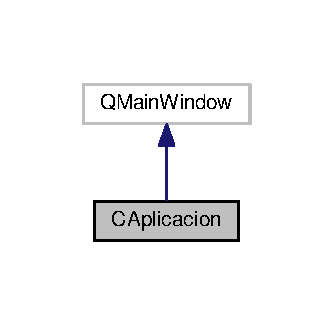
\includegraphics[width=160pt]{classCAplicacion__inherit__graph}
\end{center}
\end{figure}


Collaboration diagram for C\+Aplicacion\+:
\nopagebreak
\begin{figure}[H]
\begin{center}
\leavevmode
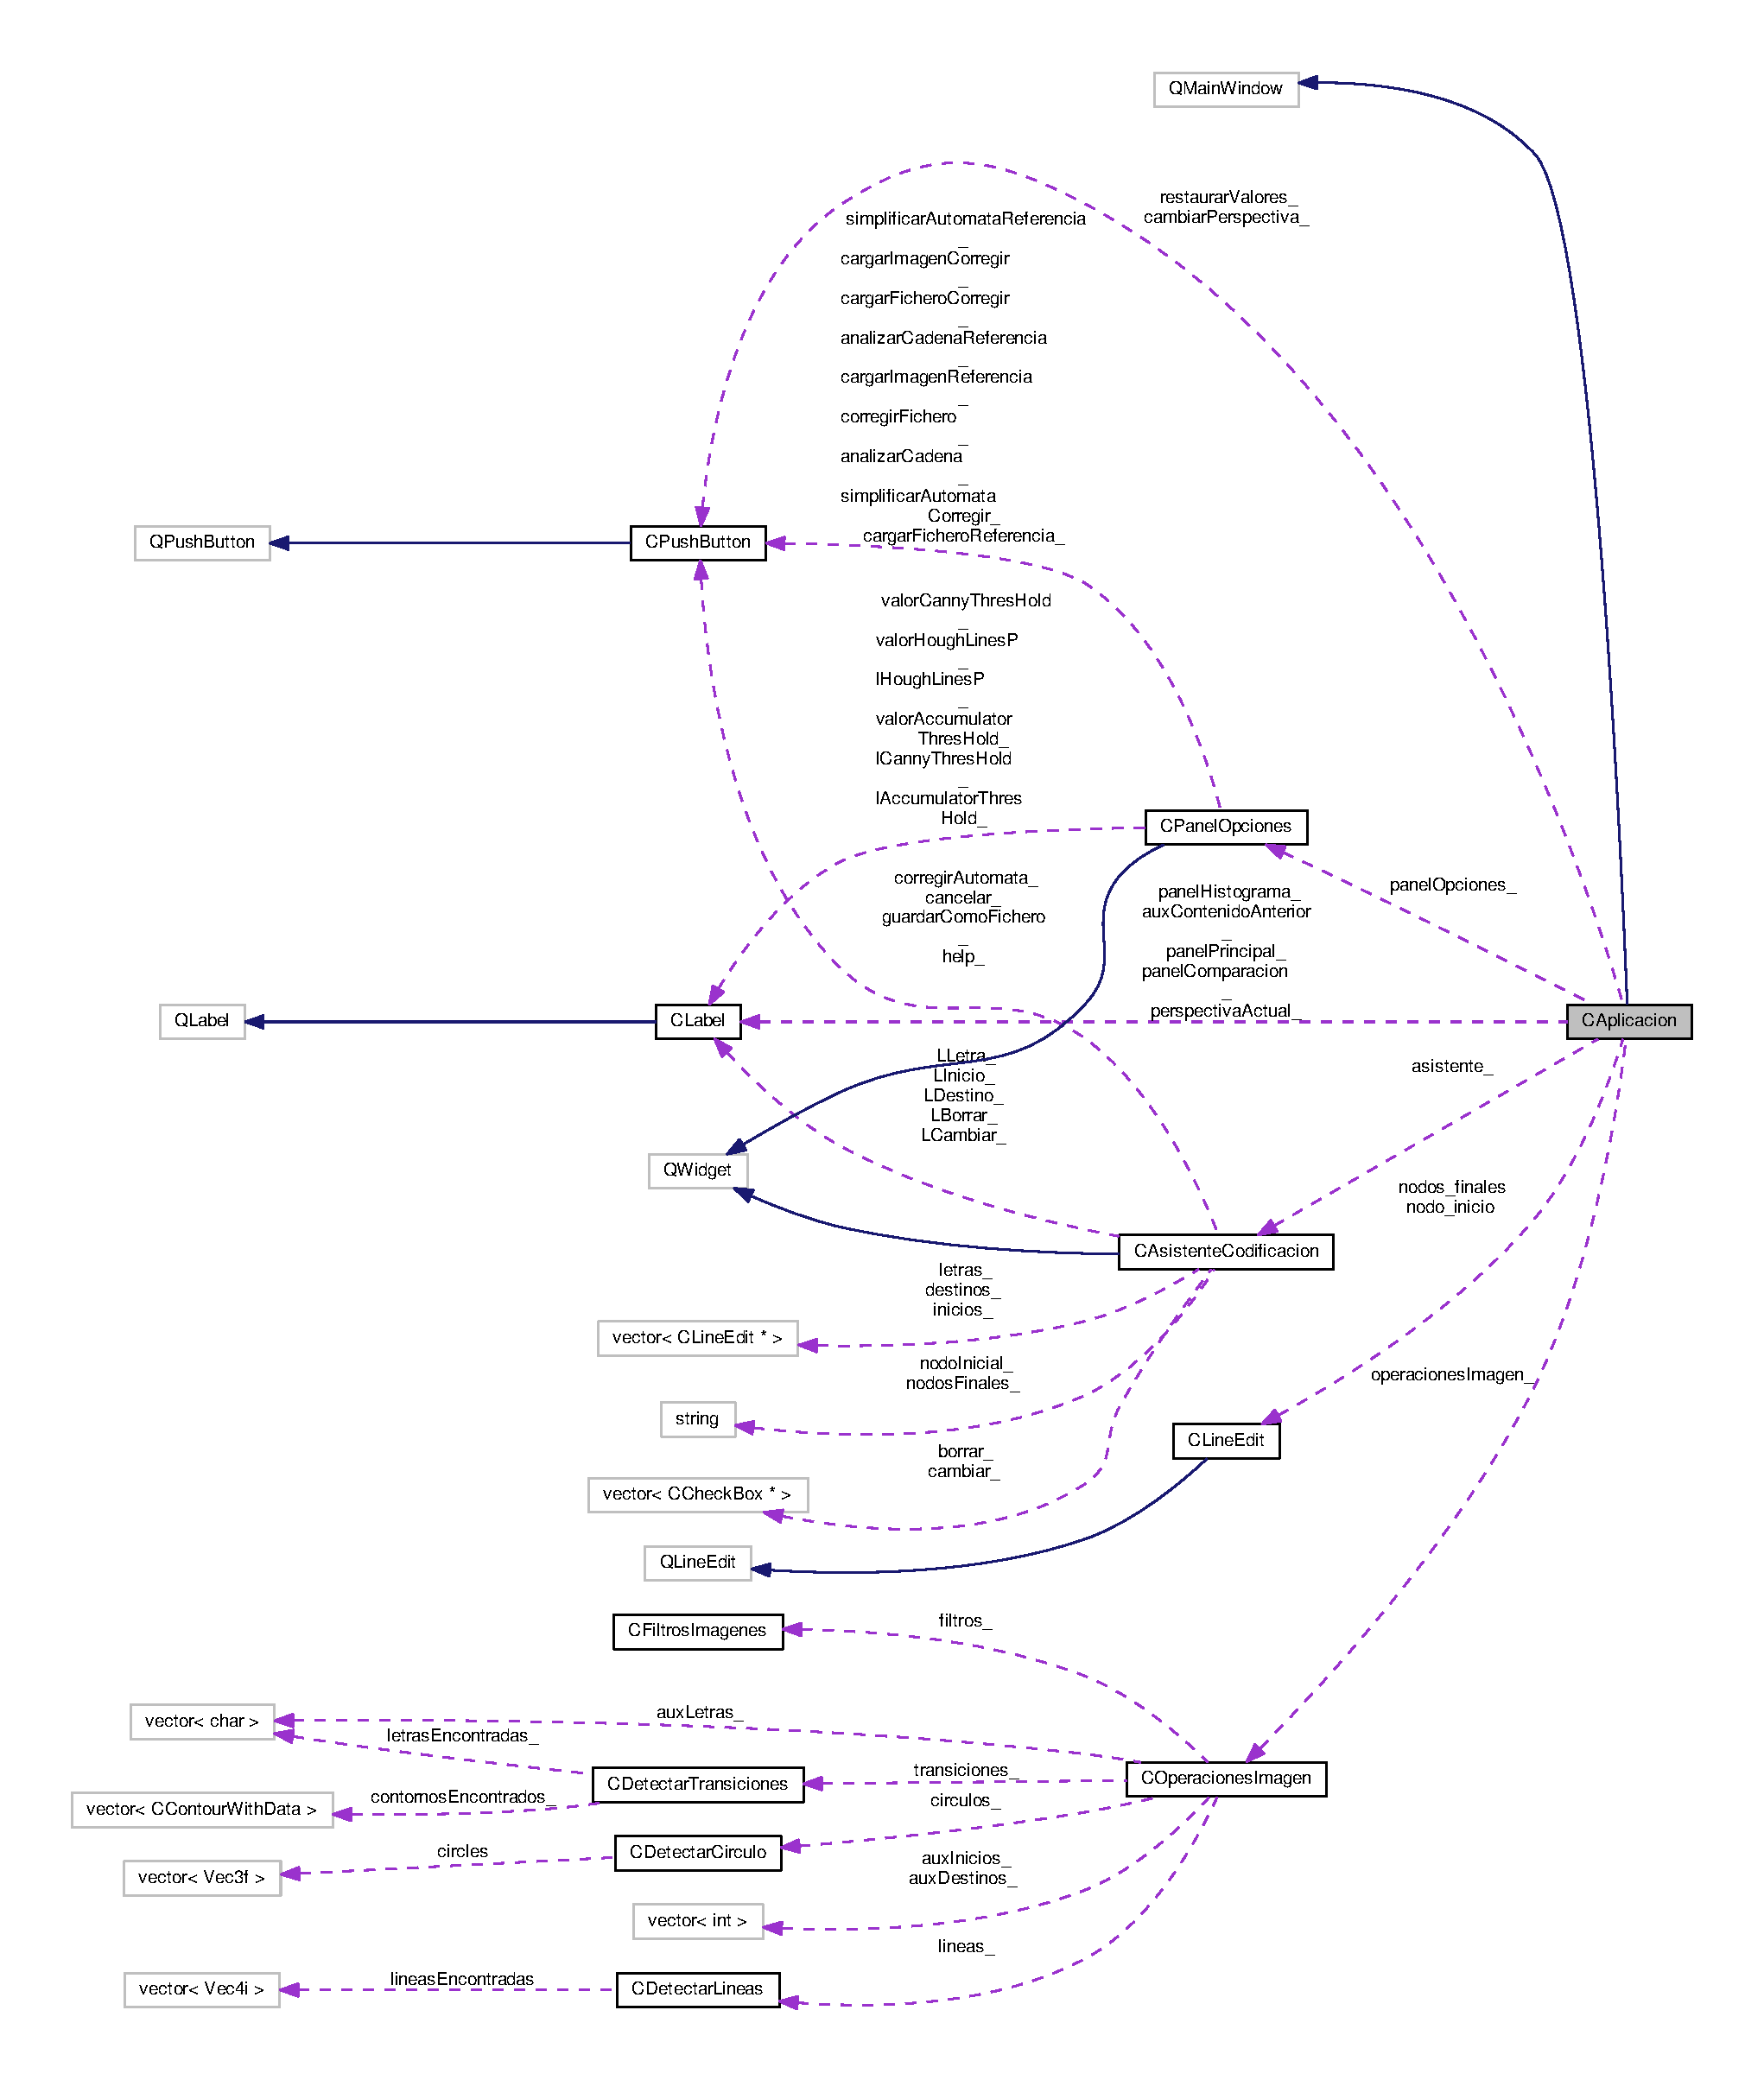
\includegraphics[width=350pt]{classCAplicacion__coll__graph}
\end{center}
\end{figure}
\subsection*{Public Slots}
\begin{DoxyCompactItemize}
\item 
void \hyperlink{classCAplicacion_ab51359b6a7881206fe6ac46e0ca982f3}{slot\+Abrir\+Imagen} ()
\begin{DoxyCompactList}\small\item\em Metodo Slot que Abre una Imagen de fichero y la coloca en el Panel Principal. \end{DoxyCompactList}\item 
void \hyperlink{classCAplicacion_a3e11d14b05a911fd2e5f5da768787ac2}{slot\+Abrir\+Fichero} ()
\begin{DoxyCompactList}\small\item\em Metodo Slot que Abre un Fichero y lo coloca en el Panel Principal. \end{DoxyCompactList}\item 
void \hyperlink{classCAplicacion_a9ac9b20ed3bd1f2750ee7649ad899f79}{slot\+About} ()
\begin{DoxyCompactList}\small\item\em Metodo Slot que Abre un Q\+Message\+Box con Informacion Relevante del Proyecto. \end{DoxyCompactList}\item 
void \hyperlink{classCAplicacion_a2950d0854e6445bf5159e7a5e65f151d}{slot\+About\+QT} ()
\begin{DoxyCompactList}\small\item\em Metodo Slot que Abre una Ventana de Informacion sobre QT Creator. \end{DoxyCompactList}\item 
void \hyperlink{classCAplicacion_af05758409bf701f83ae66333c25b8464}{slot\+Salir} ()
\begin{DoxyCompactList}\small\item\em Metodo Slot que Cierra la Aplicacion. \end{DoxyCompactList}\item 
void \hyperlink{classCAplicacion_aa7e195e4f06c864cb7c45e626d081b1c}{slot\+Detectar\+Lineas} ()
\begin{DoxyCompactList}\small\item\em Metodo Slot que detecta Lineas en la Imagen de Panel Principal a traves de operaciones\+Imagen\+\_\+ y coloca la imagen resultante en el Panel Principal de nuevo. \end{DoxyCompactList}\item 
void \hyperlink{classCAplicacion_af8fa414d46ce7a61ab9c3d19ee18a7c1}{slot\+Detectar\+Circulos} ()
\begin{DoxyCompactList}\small\item\em Metodo Slot que detecta Circulos en la Imagen de Panel Principal a traves de operaciones\+Imagen\+\_\+ y coloca la imagen resultante en el Panel Principal de nuevo. \end{DoxyCompactList}\item 
void \hyperlink{classCAplicacion_a02f4c3cd425565a9c675a10a5d9b0954}{slot\+Detectar\+Transiciones} ()
\begin{DoxyCompactList}\small\item\em Metodo Slot que detecta Transiciones en la Imagen de Panel Principal a traves de operaciones\+Imagen\+\_\+ y coloca la imagen resultante en el Panel Principal de nuevo. \end{DoxyCompactList}\item 
void \hyperlink{classCAplicacion_a87253da47e41e28e7bb911b39a885cd7}{slot\+Codificar\+Imagen} ()
\begin{DoxyCompactList}\small\item\em Metodo Slot que intenta codificar la imagen del Panel Principal. Tanto detectar\+Circulos, detectar\+Lineas y detectar\+Transiciones, deben haberse ejecutado anteriormente Se abre un asistente para confirmar los datos de la codificacion. \end{DoxyCompactList}\item 
void \hyperlink{classCAplicacion_a8855c72841e3b45c0873b9ee009df523}{slot\+Procesar\+Imagen} ()
\begin{DoxyCompactList}\small\item\em Metodo Slot que automatiza la deteccion de automatas. Detecta Lineas, Circulos, Transiciones y Codifica. \end{DoxyCompactList}\item 
void \hyperlink{classCAplicacion_a7f655c9e187d1ac28223b6bac96fd61c}{slot\+Cargar\+Imagen\+Original} ()
\begin{DoxyCompactList}\small\item\em Metodo Slot que Carga la Imagen Original de path\+Imagen\+Actual\+\_\+. \end{DoxyCompactList}\item 
void \hyperlink{classCAplicacion_a54ab1051a4cfd1a26b4081032dac96e0}{slot\+Abrir\+Fichero\+Correcto} ()
\begin{DoxyCompactList}\small\item\em Metodo Slot que Abre un Fichero mediante una ventana y lo coloca en el Panel Comparacion. \end{DoxyCompactList}\item 
void \hyperlink{classCAplicacion_a23aca6a757d7a6ce849ad52719c361f8}{slot\+Filtro\+Gray} ()
\begin{DoxyCompactList}\small\item\em Metodo Slot que utiliza el Filtro\+Gray sobre la Imagen del panel Principal. \end{DoxyCompactList}\item 
void \hyperlink{classCAplicacion_a7f09b7c407550f26bf9cf9300bfe6697}{slot\+Filtro\+Gaussiano} ()
\begin{DoxyCompactList}\small\item\em Metodo Slot que utiliza el Filtro\+Gaussiano sobre la Imagen del panel Principal. \end{DoxyCompactList}\item 
void \hyperlink{classCAplicacion_a767c2c2349db3fda16be49d16ed75e78}{slot\+Filtro\+Mediana} ()
\begin{DoxyCompactList}\small\item\em Metodo Slot que utiliza el Filtro\+Mediana sobre la Imagen del panel Principal. \end{DoxyCompactList}\item 
void \hyperlink{classCAplicacion_ac3f97714202113dc2dad77c0cea45618}{slot\+Filtro\+Sobel} ()
\begin{DoxyCompactList}\small\item\em Metodo Slot que utiliza el Filtro\+Sobel sobre la Imagen del panel Principal. \end{DoxyCompactList}\item 
void \hyperlink{classCAplicacion_ac0602f9cf86587560767791eed28585b}{slot\+Filtro\+Laplaciano} ()
\begin{DoxyCompactList}\small\item\em Metodo Slot que utiliza el Filtro\+Laplaciano sobre la Imagen del panel Principal. \end{DoxyCompactList}\item 
void \hyperlink{classCAplicacion_ae2c3ba106bbe32c000f886172c116c7a}{slot\+Histograma} ()
\begin{DoxyCompactList}\small\item\em Metodo Slot que calcula slot\+Histograma sobre la Imagen del panel Principal. \end{DoxyCompactList}\item 
void \hyperlink{classCAplicacion_a96dd498717a483124d4809dcacc7d799}{slot\+Circulos\+Canny\+Accumulator\+Hough\+LinesP} ()
\begin{DoxyCompactList}\small\item\em Metodo Slot que calcula de nuevo las detecciones hechas en la imagen si se modifica algun valor del panel Opciones. \end{DoxyCompactList}\end{DoxyCompactItemize}
\subsection*{Public Member Functions}
\begin{DoxyCompactItemize}
\item 
\hyperlink{classCAplicacion_a9b55c20439081bc5630b929b69c9fe36}{C\+Aplicacion} ()
\begin{DoxyCompactList}\small\item\em Contructor de la Clase \hyperlink{classCAplicacion}{C\+Aplicacion}. \end{DoxyCompactList}\item 
\hyperlink{classCAplicacion_a823fdda955cdfe27062d58c692b81eaf}{$\sim$\+C\+Aplicacion} ()
\begin{DoxyCompactList}\small\item\em Destructor de la Clase \hyperlink{classCAplicacion}{C\+Aplicacion}. \end{DoxyCompactList}\item 
Q\+String \hyperlink{classCAplicacion_a0cbd1aeb6fcbcc97bcb493acbaba6449}{get\+Path\+Imagen\+Actual} ()
\begin{DoxyCompactList}\small\item\em Metodo que devuelve la Path Actual de la Imagen del Panel Principal. \end{DoxyCompactList}\item 
void \hyperlink{classCAplicacion_af698484a797b35e52d029ce88390368f}{set\+Path\+Imagen\+Actual} (Q\+String new\+Path)
\begin{DoxyCompactList}\small\item\em Metodo que asigna una nueva Path de la Imagen del Panel Principal. \end{DoxyCompactList}\item 
\hyperlink{classCLabel}{C\+Label} $\ast$ \hyperlink{classCAplicacion_ae835fda5656f7ff5e6067967ed32eb09}{get\+Panel\+Principal} ()
\begin{DoxyCompactList}\small\item\em Metodo que devuelve el Panel Principal de la Aplicacion. \end{DoxyCompactList}\item 
\hyperlink{classCLabel}{C\+Label} $\ast$ \hyperlink{classCAplicacion_a8ae2ca7c0e65418c78cea44af1ba72c7}{get\+Panel\+Comparacion} ()
\begin{DoxyCompactList}\small\item\em Metodo que devuelve el Panel Comparacion de la Aplicacion. Utilizado en la correccion de automatas. \end{DoxyCompactList}\item 
\hyperlink{classCPanelOpciones}{C\+Panel\+Opciones} $\ast$ \hyperlink{classCAplicacion_a105f731579e2c93cdd5826fee8a90660}{get\+Panel\+Opciones} ()
\begin{DoxyCompactList}\small\item\em Metodo que devuelve el Panel Opciones de la Aplicacion. \end{DoxyCompactList}\item 
\hyperlink{classCLabel}{C\+Label} $\ast$ \hyperlink{classCAplicacion_a9cb501579c4725ffcc2708c824dca71c}{get\+Panel\+Histograma} ()
\begin{DoxyCompactList}\small\item\em Metodo que devuelve el panel de informacion de la Aplicacion. \end{DoxyCompactList}\item 
Q\+Grid\+Layout $\ast$ \hyperlink{classCAplicacion_af8687ea0c860ca7df1f0189f932ea93d}{get\+Layout} ()
\begin{DoxyCompactList}\small\item\em Metodo que devuelve el layout de la Aplicacion. \end{DoxyCompactList}\item 
Q\+Menu\+Bar $\ast$ \hyperlink{classCAplicacion_a8b8ddfe3c7112cd0645926fe3c628c7f}{get\+Menu\+Bar} ()
\begin{DoxyCompactList}\small\item\em Metodo que devuelve el Menu de la Aplicacion. \end{DoxyCompactList}\item 
Q\+Menu $\ast$ \hyperlink{classCAplicacion_a9eb944127e33a2f045b59875c1920756}{get\+Menu\+Archivo} ()
\begin{DoxyCompactList}\small\item\em Metodo que devuelve el submenu Archivo del Menu de la Aplicacion. \end{DoxyCompactList}\item 
Q\+Menu $\ast$ \hyperlink{classCAplicacion_a283d64e238855df344498c8aed50ff96}{get\+Menu\+Editar} ()
\begin{DoxyCompactList}\small\item\em Metodo que devuelve el submenu Editar del Menu de la Aplicacion. \end{DoxyCompactList}\item 
Q\+Menu $\ast$ \hyperlink{classCAplicacion_a67443b72909b19dfae9f2d322b2eaa7e}{get\+Menu\+Correccion} ()
\begin{DoxyCompactList}\small\item\em Metodo que devuelve el submenu Correccion del Menu de la Aplicacion. \end{DoxyCompactList}\item 
Q\+Menu $\ast$ \hyperlink{classCAplicacion_aa234ca246ac29bfca8c8f8fc39e07206}{get\+Menu\+Filtro} ()
\begin{DoxyCompactList}\small\item\em Metodo que devuelve el submenu Filtro del Menu de la Aplicacion. \end{DoxyCompactList}\item 
Q\+Tool\+Bar $\ast$ \hyperlink{classCAplicacion_a7cc8e6f81a363c5fec003c811e7f2618}{get\+Tool\+Bar} ()
\begin{DoxyCompactList}\small\item\em Metodo que devuelve el Tool\+Bar de la Aplicacion. \end{DoxyCompactList}\item 
\hyperlink{classCLineEdit}{C\+Line\+Edit} $\ast$ \hyperlink{classCAplicacion_af85f5505cf86de4ea460765b0032fa4f}{get\+Nodo\+Inicio} ()
\begin{DoxyCompactList}\small\item\em Metodo que devuelve el campo \hyperlink{classCLineEdit}{C\+Line\+Edit}, nodo de inicio. Este se introducirá en la ventana. \end{DoxyCompactList}\item 
\hyperlink{classCLineEdit}{C\+Line\+Edit} $\ast$ \hyperlink{classCAplicacion_a17a77e146a8a785cbf92158c9b7240df}{get\+Nodos\+Finales} ()
\begin{DoxyCompactList}\small\item\em Metodo que devuelve el campo \hyperlink{classCLineEdit}{C\+Line\+Edit}, nodos finales. Estos se introduciran en la ventana. \end{DoxyCompactList}\item 
Q\+Combo\+Box $\ast$ \hyperlink{classCAplicacion_a41b85abfacd73ff66a345d08b934bc45}{get\+Alfabeto\+Actual} ()
\begin{DoxyCompactList}\small\item\em Metodo que devuelve el campo Q\+Combo\+Box, alfabeto actual, se elige en la ventana si es alfabetico o numerico. \end{DoxyCompactList}\item 
Q\+Action $\ast$ \hyperlink{classCAplicacion_a8016e78de08ca0dfb1e74750a0fcacf1}{get\+Action\+Abrir\+Imagen} ()
\begin{DoxyCompactList}\small\item\em Metodo que devuelve la Accion Abrir Imagen. \end{DoxyCompactList}\item 
Q\+Action $\ast$ \hyperlink{classCAplicacion_adf620887eb4c888ec7bbe1178df9d307}{get\+Action\+Abrir\+Fichero} ()
\begin{DoxyCompactList}\small\item\em Metodo que devuelve la Accion Abrir Fichero. \end{DoxyCompactList}\item 
Q\+Action $\ast$ \hyperlink{classCAplicacion_a46ac4ceff3c82283f159c467a5cde6d2}{get\+Action\+About} ()
\begin{DoxyCompactList}\small\item\em Metodo que devuelve la Accion About. \end{DoxyCompactList}\item 
Q\+Action $\ast$ \hyperlink{classCAplicacion_a8f0d5c5ad866644453dcedb5a45c2044}{get\+Action\+About\+QT} ()
\begin{DoxyCompactList}\small\item\em Metodo que devuelve la Accion About QT. \end{DoxyCompactList}\item 
Q\+Action $\ast$ \hyperlink{classCAplicacion_a0326521d3aacf2c129f8b63ce6dd51b1}{get\+Action\+Salir} ()
\begin{DoxyCompactList}\small\item\em Metodo que devuelve la Accion Salir. \end{DoxyCompactList}\item 
Q\+Action $\ast$ \hyperlink{classCAplicacion_a44d0d263883784b27191c34493a56154}{get\+Action\+Detectar\+Lineas} ()
\begin{DoxyCompactList}\small\item\em Metodo que devuelve la Accion Detectar Lineas. \end{DoxyCompactList}\item 
Q\+Action $\ast$ \hyperlink{classCAplicacion_af4811205741a71ee2f897491119e2a85}{get\+Action\+Detectar\+Circulos} ()
\begin{DoxyCompactList}\small\item\em Metodo que devuelve la Accion Detectar\+Circulos. \end{DoxyCompactList}\item 
Q\+Action $\ast$ \hyperlink{classCAplicacion_a7ae388e051747fbc0aa9a47696d5d5da}{get\+Action\+Detectar\+Transiciones} ()
\begin{DoxyCompactList}\small\item\em Metodo que devuelve la Accion Detectar Transiciones. \end{DoxyCompactList}\item 
Q\+Action $\ast$ \hyperlink{classCAplicacion_a298625cc516fc874fd53f73fcf2ca883}{get\+Action\+Codificar\+Imagen} ()
\begin{DoxyCompactList}\small\item\em Metodo que devuelve la Accion Codificar Imagen. \end{DoxyCompactList}\item 
Q\+Action $\ast$ \hyperlink{classCAplicacion_aba97c29b89e7c7b1163e3e3cde189e4b}{get\+Action\+Procesar\+Imagen} ()
\begin{DoxyCompactList}\small\item\em Metodo que devuelve la Accion Procesar Imagen. \end{DoxyCompactList}\item 
Q\+Action $\ast$ \hyperlink{classCAplicacion_a00c192ecc07c4690802eb38c1f48731b}{get\+Action\+Cargar\+Imagen\+Original} ()
\begin{DoxyCompactList}\small\item\em Metodo que devuelve la Accion Cargar Imagen Original, leida desde get Path Imagen Actual. \end{DoxyCompactList}\item 
Q\+Action $\ast$ \hyperlink{classCAplicacion_a4b70b7b2987f70046fa1ea8c4ed02990}{get\+Action\+Abrir\+Fichero\+Correcto} ()
\begin{DoxyCompactList}\small\item\em Metodo que devuelve la Accion Abrir Fichero Correcto. \end{DoxyCompactList}\item 
Q\+Action $\ast$ \hyperlink{classCAplicacion_a45304c1304bedcde6c42cf3f9c7b4f19}{get\+Action\+Filtro\+Gray} ()
\begin{DoxyCompactList}\small\item\em Metodo que devuelve la Accion Filtro Gray. \end{DoxyCompactList}\item 
Q\+Action $\ast$ \hyperlink{classCAplicacion_a5929e30f259ac77d0f72a8fbd1cb89c7}{get\+Action\+Filtro\+Gaussiano} ()
\begin{DoxyCompactList}\small\item\em Metodo que devuelve la Accion Filtro Gaussiano. \end{DoxyCompactList}\item 
Q\+Action $\ast$ \hyperlink{classCAplicacion_a8439aed96fa9a5a80f37be6b2dd67f4b}{get\+Action\+Filtro\+Mediana} ()
\begin{DoxyCompactList}\small\item\em Metodo que devuelve la Accion Filtro Mediana. \end{DoxyCompactList}\item 
Q\+Action $\ast$ \hyperlink{classCAplicacion_a4c7a3e1bf75bee8ba9a8c6a092c4b55e}{get\+Action\+Filtro\+Sobel} ()
\begin{DoxyCompactList}\small\item\em Metodo que devuelve la Accion Filtro Sobel. \end{DoxyCompactList}\item 
Q\+Action $\ast$ \hyperlink{classCAplicacion_a9e3487513378f95c231dd8806222f126}{get\+Action\+Filtro\+Laplaciano} ()
\begin{DoxyCompactList}\small\item\em Metodo que devuelve la Accion Filtro Laplaciano. \end{DoxyCompactList}\item 
Q\+Action $\ast$ \hyperlink{classCAplicacion_a297c40499e1dc0a7fe428846df8b37b6}{get\+Action\+Histograma} ()
\begin{DoxyCompactList}\small\item\em Metodo que devuelve la Accion Histograma. \end{DoxyCompactList}\item 
\hyperlink{classCOperacionesImagen}{C\+Operaciones\+Imagen} $\ast$ \hyperlink{classCAplicacion_acf0f5ed748482f7957bee4db4dadf840}{get\+Operaciones\+Imagen} ()
\begin{DoxyCompactList}\small\item\em Metodo que devuelve el atributo operaciones\+Imagen\+\_\+. \end{DoxyCompactList}\end{DoxyCompactItemize}
\subsection*{Private Member Functions}
\begin{DoxyCompactItemize}
\item 
bool \hyperlink{classCAplicacion_a7802ee67b172b877ddd0f3ac99a7d96e}{load\+File} (const Q\+String \&file\+Name)
\begin{DoxyCompactList}\small\item\em Metodo para Abrir Imagen, utilizado en slot\+Abrir\+Imagen. \end{DoxyCompactList}\item 
void \hyperlink{classCAplicacion_a9d66dd978838dd5b4c99ddb02a9e43a1}{inicializar\+Ventana\+Abrir\+Imagen} (Q\+File\+Dialog \&, Q\+File\+Dialog\+::\+Accept\+Mode)
\begin{DoxyCompactList}\small\item\em Metodo que inicializa la ventana Abrir Imagen en la carpeta Imagen por defecto Ordena los archivos del buscador y filtra por png. \end{DoxyCompactList}\item 
Q\+String \hyperlink{classCAplicacion_a66f53bbf6ae42a812a449bd96610e702}{ventana\+Abrir\+Fichero} ()
\begin{DoxyCompactList}\small\item\em Metodo que abre un fichero deseado mediante asistente de ventana. Filtra por text Files y directorio por defecto. Mis documentos. \end{DoxyCompactList}\end{DoxyCompactItemize}
\subsection*{Private Attributes}
\begin{DoxyCompactItemize}
\item 
Q\+Image \hyperlink{classCAplicacion_a0d02a7838c0974bffc76e8dd08848dc9}{imagen\+Panel\+Principal}
\begin{DoxyCompactList}\small\item\em Imagen actual del panel principal. \end{DoxyCompactList}\item 
Q\+String \hyperlink{classCAplicacion_a990b6780cd5e1d941f01e7df20958587}{path\+Imagen\+Actual\+\_\+}
\begin{DoxyCompactList}\small\item\em Ruta de la imagen actual del panel principal. \end{DoxyCompactList}\item 
\hyperlink{classCLabel}{C\+Label} $\ast$ \hyperlink{classCAplicacion_ac795b4ce529859a5d5c03e15ed78d967}{panel\+Principal\+\_\+}
\begin{DoxyCompactList}\small\item\em Panel Principal de la Aplicacion. \end{DoxyCompactList}\item 
\hyperlink{classCLabel}{C\+Label} $\ast$ \hyperlink{classCAplicacion_a16f1c9d4fd9168f0787c210588a048be}{panel\+Comparacion\+\_\+}
\begin{DoxyCompactList}\small\item\em Panel secundario utilizado para introducir un fichero en la etapa de correccion de automatas. \end{DoxyCompactList}\item 
\hyperlink{classCPanelOpciones}{C\+Panel\+Opciones} $\ast$ \hyperlink{classCAplicacion_adc38c4ae217096b72da9911d6cf39f47}{panel\+Opciones\+\_\+}
\begin{DoxyCompactList}\small\item\em Panel Opciones de la Aplicacion. \end{DoxyCompactList}\item 
\hyperlink{classCLabel}{C\+Label} $\ast$ \hyperlink{classCAplicacion_a5edbe0644420ff42d80a2a5d247c69eb}{panel\+Histograma\+\_\+}
\begin{DoxyCompactList}\small\item\em Panel Informacion de la Aplicacion. \end{DoxyCompactList}\item 
Q\+Grid\+Layout $\ast$ \hyperlink{classCAplicacion_a135b700bb291de086b00bcc4481ffc8b}{layout\+\_\+}
\begin{DoxyCompactList}\small\item\em Layout de la aplicacion, formato Grid\+Layout. \end{DoxyCompactList}\item 
Q\+Menu\+Bar $\ast$ \hyperlink{classCAplicacion_af1ac43fa5f82c2512f211fc0dbb00a3a}{menu\+\_\+}
\begin{DoxyCompactList}\small\item\em Menu de la aplicacion, contiene Archivo, Editar, Correccion y Filtros. \end{DoxyCompactList}\item 
Q\+Menu $\ast$ \hyperlink{classCAplicacion_abdf7a15d27725756e59d4408267d4688}{menu\+Archivo\+\_\+}
\begin{DoxyCompactList}\small\item\em Submenu Archivo de la Aplicacion. \end{DoxyCompactList}\item 
Q\+Menu $\ast$ \hyperlink{classCAplicacion_a9753ee6650d3a8922650b09b70fe15b9}{menu\+Editar\+\_\+}
\begin{DoxyCompactList}\small\item\em Submenu Editar de la Aplicacion. \end{DoxyCompactList}\item 
Q\+Menu $\ast$ \hyperlink{classCAplicacion_acb53cba72e72d1b6feb8203a4942b436}{menu\+Correccion\+\_\+}
\begin{DoxyCompactList}\small\item\em Submenu Correcion de la Aplicacion. \end{DoxyCompactList}\item 
Q\+Menu $\ast$ \hyperlink{classCAplicacion_af9dedeec60356a055cb899e5f8a447b8}{menu\+Filtro\+\_\+}
\begin{DoxyCompactList}\small\item\em Submenu Filtro de la Aplicacion. \end{DoxyCompactList}\item 
Q\+Action $\ast$ \hyperlink{classCAplicacion_ac7f0a3871355c19d02bf87f36322cee7}{action\+Abrir\+Imagen\+\_\+}
\begin{DoxyCompactList}\small\item\em Accion Abrir Imagen del Submenu Archivo. \end{DoxyCompactList}\item 
Q\+Action $\ast$ \hyperlink{classCAplicacion_a4fa499b5119ad7bcc86f53ace963cbbd}{action\+Abrir\+Fichero\+\_\+}
\begin{DoxyCompactList}\small\item\em Accion Abrir Fichero del Submenu Archivo. \end{DoxyCompactList}\item 
Q\+Action $\ast$ \hyperlink{classCAplicacion_ac42dda1caacc0506c7015c79fde8416f}{action\+About\+\_\+}
\begin{DoxyCompactList}\small\item\em Accion About del Submenu Archivo. \end{DoxyCompactList}\item 
Q\+Action $\ast$ \hyperlink{classCAplicacion_af0ed23ead2d1c3aea79b724c3cb70249}{action\+About\+Q\+T\+\_\+}
\begin{DoxyCompactList}\small\item\em Accion About Qt del Submenu Archivo. \end{DoxyCompactList}\item 
Q\+Action $\ast$ \hyperlink{classCAplicacion_ac878000751c05f9491a9de6671e6cde0}{action\+Salir\+\_\+}
\begin{DoxyCompactList}\small\item\em Accion Salir del Submenu Archivo. \end{DoxyCompactList}\item 
Q\+Action $\ast$ \hyperlink{classCAplicacion_a5b6d0af534cc0f64dfb7598faa30f3ae}{action\+Detectar\+Lineas\+\_\+}
\begin{DoxyCompactList}\small\item\em Accion Detectar Lineas del Submenu Editar. \end{DoxyCompactList}\item 
Q\+Action $\ast$ \hyperlink{classCAplicacion_ab4c2fb6ecc5d7c21a1f181f0f0af2830}{action\+Detectar\+Circulos\+\_\+}
\begin{DoxyCompactList}\small\item\em Accion Detectar Circulos del Submenu Editar. \end{DoxyCompactList}\item 
Q\+Action $\ast$ \hyperlink{classCAplicacion_acda82e41d91a94e32bbfa21965338f5a}{action\+Detectar\+Transiciones\+\_\+}
\begin{DoxyCompactList}\small\item\em Accion Detectar Transiciones del Submenu Editar. \end{DoxyCompactList}\item 
Q\+Action $\ast$ \hyperlink{classCAplicacion_a06464c87dd4924cc8bb92f946239f603}{action\+Codificar\+Imagen\+\_\+}
\begin{DoxyCompactList}\small\item\em Accion Codificar Imagen del Submenu Editar. \end{DoxyCompactList}\item 
Q\+Action $\ast$ \hyperlink{classCAplicacion_a9fa952c19f9da356432fae60a40cdced}{action\+Procesar\+Imagen\+\_\+}
\begin{DoxyCompactList}\small\item\em Accion Procesar Imagen del Submenu Editar. Procesar\+Imagen = Detectar\+Lineas() + Detectar\+Circulos() + Detectar\+Transiciones() + Codificar\+Imagen() \end{DoxyCompactList}\item 
Q\+Action $\ast$ \hyperlink{classCAplicacion_a3768f71b55ac5e2d77fed775d8ebce74}{action\+Cargar\+Imagen\+Original\+\_\+}
\begin{DoxyCompactList}\small\item\em Accion Cargar Imagen imagen\+Panel\+Principal\+\_\+ . Submenu Editar. \end{DoxyCompactList}\item 
Q\+Action $\ast$ \hyperlink{classCAplicacion_abd9f33aa366727875ab9c798e1a4695c}{action\+Abrir\+Fichero\+Correcto\+\_\+}
\begin{DoxyCompactList}\small\item\em Accion Abrir Fichero Correcto. Submenu Correccion. \end{DoxyCompactList}\item 
Q\+Action $\ast$ \hyperlink{classCAplicacion_a62326cfe231c222d4d3411b4f9a5fc81}{action\+Filtro\+Gray\+\_\+}
\begin{DoxyCompactList}\small\item\em Accion Filtro Gray. Submenu Filtro. \end{DoxyCompactList}\item 
Q\+Action $\ast$ \hyperlink{classCAplicacion_ae6827414fe74e31b2216ec04f61ad21f}{action\+Filtro\+Gaussiano\+\_\+}
\begin{DoxyCompactList}\small\item\em Accion Filtro Gaussiano. Submenu Filtro. \end{DoxyCompactList}\item 
Q\+Action $\ast$ \hyperlink{classCAplicacion_a7121918f17fc9640c91f26961f7ee221}{action\+Filtro\+Mediana\+\_\+}
\begin{DoxyCompactList}\small\item\em Accion Filtro Mediana. Submenu Filtro. \end{DoxyCompactList}\item 
Q\+Action $\ast$ \hyperlink{classCAplicacion_a96511c94f6a4a6da0466d460272f56bf}{action\+Filtro\+Sobel\+\_\+}
\begin{DoxyCompactList}\small\item\em Accion Filtro Sobel. Submenu Filtro. \end{DoxyCompactList}\item 
Q\+Action $\ast$ \hyperlink{classCAplicacion_ad1cce3c330ee913f1129d19bba5f22f0}{action\+Filtro\+Laplaciano\+\_\+}
\begin{DoxyCompactList}\small\item\em Accion Filtro Laplaciano. Submenu Filtro. \end{DoxyCompactList}\item 
Q\+Action $\ast$ \hyperlink{classCAplicacion_a60f0707037ad02949ff17858729faff2}{action\+Histograma\+\_\+}
\begin{DoxyCompactList}\small\item\em Accion Filtro Histograma. Submenu Filtro. \end{DoxyCompactList}\item 
Q\+Tool\+Bar $\ast$ \hyperlink{classCAplicacion_a2dca58bda4c34c0f76d8c95fcbba064c}{toolbar\+\_\+}
\begin{DoxyCompactList}\small\item\em Toolbal de la aplicacion. Opciones de Deteccion de la imagen. \end{DoxyCompactList}\item 
\hyperlink{classCLineEdit}{C\+Line\+Edit} $\ast$ \hyperlink{classCAplicacion_a9d3e345fc25efeaf8a160daf22206a8e}{nodo\+\_\+inicio}
\begin{DoxyCompactList}\small\item\em Q\+Line\+Edit para introducir el nodo de inicio del automata. \end{DoxyCompactList}\item 
\hyperlink{classCLineEdit}{C\+Line\+Edit} $\ast$ \hyperlink{classCAplicacion_a483026f954a5a26ddd9ded5863c61b9a}{nodos\+\_\+finales}
\begin{DoxyCompactList}\small\item\em Q\+Line\+Edit para introducir los nodos finales del automata. \end{DoxyCompactList}\item 
Q\+Combo\+Box $\ast$ \hyperlink{classCAplicacion_a2bc2fca932b919c027f2c4a35f837de0}{alfabeto\+\_\+}
\begin{DoxyCompactList}\small\item\em Q\+Combo\+Box para definir el alfabeto. 0 -\/$>$ alfabeto a, b, c 1 -\/$>$ Alfabeto numerico. \end{DoxyCompactList}\item 
\hyperlink{classCOperacionesImagen}{C\+Operaciones\+Imagen} $\ast$ \hyperlink{classCAplicacion_a58596bdd1d1e018bcb8bd58b64de538e}{operaciones\+Imagen\+\_\+}
\begin{DoxyCompactList}\small\item\em Clase para aplicar operaciones sobre la Imagen. Deteccion, filtros y Asistente. \end{DoxyCompactList}\end{DoxyCompactItemize}


\subsection{Detailed Description}
Clase Aplicacion con ventana principal de la aplicacion Consta de 3 Paneles. Principal, Opciones e Histograma Si se utiliza la funcionalidad Codificar, ese panel cambia de forma T\+E\+R\+M\+I\+N\+AR. 

\subsection{Constructor \& Destructor Documentation}
\index{C\+Aplicacion@{C\+Aplicacion}!C\+Aplicacion@{C\+Aplicacion}}
\index{C\+Aplicacion@{C\+Aplicacion}!C\+Aplicacion@{C\+Aplicacion}}
\subsubsection[{\texorpdfstring{C\+Aplicacion()}{CAplicacion()}}]{\setlength{\rightskip}{0pt plus 5cm}C\+Aplicacion\+::\+C\+Aplicacion (
\begin{DoxyParamCaption}
{}
\end{DoxyParamCaption}
)}\hypertarget{classCAplicacion_a9b55c20439081bc5630b929b69c9fe36}{}\label{classCAplicacion_a9b55c20439081bc5630b929b69c9fe36}


Contructor de la Clase \hyperlink{classCAplicacion}{C\+Aplicacion}. 

Creamos los Paneles de la Aplicacion y su disposicion

Creamos el Menu

Shortcuts

Añadimos Toolbar

conexiones con slots \index{C\+Aplicacion@{C\+Aplicacion}!````~C\+Aplicacion@{$\sim$\+C\+Aplicacion}}
\index{````~C\+Aplicacion@{$\sim$\+C\+Aplicacion}!C\+Aplicacion@{C\+Aplicacion}}
\subsubsection[{\texorpdfstring{$\sim$\+C\+Aplicacion()}{~CAplicacion()}}]{\setlength{\rightskip}{0pt plus 5cm}C\+Aplicacion\+::$\sim$\+C\+Aplicacion (
\begin{DoxyParamCaption}
{}
\end{DoxyParamCaption}
)}\hypertarget{classCAplicacion_a823fdda955cdfe27062d58c692b81eaf}{}\label{classCAplicacion_a823fdda955cdfe27062d58c692b81eaf}


Destructor de la Clase \hyperlink{classCAplicacion}{C\+Aplicacion}. 



\subsection{Member Function Documentation}
\index{C\+Aplicacion@{C\+Aplicacion}!get\+Action\+About@{get\+Action\+About}}
\index{get\+Action\+About@{get\+Action\+About}!C\+Aplicacion@{C\+Aplicacion}}
\subsubsection[{\texorpdfstring{get\+Action\+About()}{getActionAbout()}}]{\setlength{\rightskip}{0pt plus 5cm}Q\+Action $\ast$ C\+Aplicacion\+::get\+Action\+About (
\begin{DoxyParamCaption}
{}
\end{DoxyParamCaption}
)}\hypertarget{classCAplicacion_a46ac4ceff3c82283f159c467a5cde6d2}{}\label{classCAplicacion_a46ac4ceff3c82283f159c467a5cde6d2}


Metodo que devuelve la Accion About. 

\begin{DoxyReturn}{Returns}
Q\+Action 
\end{DoxyReturn}
\index{C\+Aplicacion@{C\+Aplicacion}!get\+Action\+About\+QT@{get\+Action\+About\+QT}}
\index{get\+Action\+About\+QT@{get\+Action\+About\+QT}!C\+Aplicacion@{C\+Aplicacion}}
\subsubsection[{\texorpdfstring{get\+Action\+About\+Q\+T()}{getActionAboutQT()}}]{\setlength{\rightskip}{0pt plus 5cm}Q\+Action $\ast$ C\+Aplicacion\+::get\+Action\+About\+QT (
\begin{DoxyParamCaption}
{}
\end{DoxyParamCaption}
)}\hypertarget{classCAplicacion_a8f0d5c5ad866644453dcedb5a45c2044}{}\label{classCAplicacion_a8f0d5c5ad866644453dcedb5a45c2044}


Metodo que devuelve la Accion About QT. 

\begin{DoxyReturn}{Returns}
Q\+Action 
\end{DoxyReturn}
\index{C\+Aplicacion@{C\+Aplicacion}!get\+Action\+Abrir\+Fichero@{get\+Action\+Abrir\+Fichero}}
\index{get\+Action\+Abrir\+Fichero@{get\+Action\+Abrir\+Fichero}!C\+Aplicacion@{C\+Aplicacion}}
\subsubsection[{\texorpdfstring{get\+Action\+Abrir\+Fichero()}{getActionAbrirFichero()}}]{\setlength{\rightskip}{0pt plus 5cm}Q\+Action $\ast$ C\+Aplicacion\+::get\+Action\+Abrir\+Fichero (
\begin{DoxyParamCaption}
{}
\end{DoxyParamCaption}
)}\hypertarget{classCAplicacion_adf620887eb4c888ec7bbe1178df9d307}{}\label{classCAplicacion_adf620887eb4c888ec7bbe1178df9d307}


Metodo que devuelve la Accion Abrir Fichero. 

\begin{DoxyReturn}{Returns}
Q\+Action 
\end{DoxyReturn}
\index{C\+Aplicacion@{C\+Aplicacion}!get\+Action\+Abrir\+Fichero\+Correcto@{get\+Action\+Abrir\+Fichero\+Correcto}}
\index{get\+Action\+Abrir\+Fichero\+Correcto@{get\+Action\+Abrir\+Fichero\+Correcto}!C\+Aplicacion@{C\+Aplicacion}}
\subsubsection[{\texorpdfstring{get\+Action\+Abrir\+Fichero\+Correcto()}{getActionAbrirFicheroCorrecto()}}]{\setlength{\rightskip}{0pt plus 5cm}Q\+Action $\ast$ C\+Aplicacion\+::get\+Action\+Abrir\+Fichero\+Correcto (
\begin{DoxyParamCaption}
{}
\end{DoxyParamCaption}
)}\hypertarget{classCAplicacion_a4b70b7b2987f70046fa1ea8c4ed02990}{}\label{classCAplicacion_a4b70b7b2987f70046fa1ea8c4ed02990}


Metodo que devuelve la Accion Abrir Fichero Correcto. 

\begin{DoxyReturn}{Returns}
Q\+Action 
\end{DoxyReturn}
\index{C\+Aplicacion@{C\+Aplicacion}!get\+Action\+Abrir\+Imagen@{get\+Action\+Abrir\+Imagen}}
\index{get\+Action\+Abrir\+Imagen@{get\+Action\+Abrir\+Imagen}!C\+Aplicacion@{C\+Aplicacion}}
\subsubsection[{\texorpdfstring{get\+Action\+Abrir\+Imagen()}{getActionAbrirImagen()}}]{\setlength{\rightskip}{0pt plus 5cm}Q\+Action $\ast$ C\+Aplicacion\+::get\+Action\+Abrir\+Imagen (
\begin{DoxyParamCaption}
{}
\end{DoxyParamCaption}
)}\hypertarget{classCAplicacion_a8016e78de08ca0dfb1e74750a0fcacf1}{}\label{classCAplicacion_a8016e78de08ca0dfb1e74750a0fcacf1}


Metodo que devuelve la Accion Abrir Imagen. 

\begin{DoxyReturn}{Returns}
Q\+Action 
\end{DoxyReturn}
\index{C\+Aplicacion@{C\+Aplicacion}!get\+Action\+Cargar\+Imagen\+Original@{get\+Action\+Cargar\+Imagen\+Original}}
\index{get\+Action\+Cargar\+Imagen\+Original@{get\+Action\+Cargar\+Imagen\+Original}!C\+Aplicacion@{C\+Aplicacion}}
\subsubsection[{\texorpdfstring{get\+Action\+Cargar\+Imagen\+Original()}{getActionCargarImagenOriginal()}}]{\setlength{\rightskip}{0pt plus 5cm}Q\+Action $\ast$ C\+Aplicacion\+::get\+Action\+Cargar\+Imagen\+Original (
\begin{DoxyParamCaption}
{}
\end{DoxyParamCaption}
)}\hypertarget{classCAplicacion_a00c192ecc07c4690802eb38c1f48731b}{}\label{classCAplicacion_a00c192ecc07c4690802eb38c1f48731b}


Metodo que devuelve la Accion Cargar Imagen Original, leida desde get Path Imagen Actual. 

\begin{DoxyReturn}{Returns}
Q\+Action 
\end{DoxyReturn}
\index{C\+Aplicacion@{C\+Aplicacion}!get\+Action\+Codificar\+Imagen@{get\+Action\+Codificar\+Imagen}}
\index{get\+Action\+Codificar\+Imagen@{get\+Action\+Codificar\+Imagen}!C\+Aplicacion@{C\+Aplicacion}}
\subsubsection[{\texorpdfstring{get\+Action\+Codificar\+Imagen()}{getActionCodificarImagen()}}]{\setlength{\rightskip}{0pt plus 5cm}Q\+Action $\ast$ C\+Aplicacion\+::get\+Action\+Codificar\+Imagen (
\begin{DoxyParamCaption}
{}
\end{DoxyParamCaption}
)}\hypertarget{classCAplicacion_a298625cc516fc874fd53f73fcf2ca883}{}\label{classCAplicacion_a298625cc516fc874fd53f73fcf2ca883}


Metodo que devuelve la Accion Codificar Imagen. 

\begin{DoxyReturn}{Returns}
Q\+Action 
\end{DoxyReturn}
\index{C\+Aplicacion@{C\+Aplicacion}!get\+Action\+Detectar\+Circulos@{get\+Action\+Detectar\+Circulos}}
\index{get\+Action\+Detectar\+Circulos@{get\+Action\+Detectar\+Circulos}!C\+Aplicacion@{C\+Aplicacion}}
\subsubsection[{\texorpdfstring{get\+Action\+Detectar\+Circulos()}{getActionDetectarCirculos()}}]{\setlength{\rightskip}{0pt plus 5cm}Q\+Action $\ast$ C\+Aplicacion\+::get\+Action\+Detectar\+Circulos (
\begin{DoxyParamCaption}
{}
\end{DoxyParamCaption}
)}\hypertarget{classCAplicacion_af4811205741a71ee2f897491119e2a85}{}\label{classCAplicacion_af4811205741a71ee2f897491119e2a85}


Metodo que devuelve la Accion Detectar\+Circulos. 

\begin{DoxyReturn}{Returns}
Q\+Action 
\end{DoxyReturn}
\index{C\+Aplicacion@{C\+Aplicacion}!get\+Action\+Detectar\+Lineas@{get\+Action\+Detectar\+Lineas}}
\index{get\+Action\+Detectar\+Lineas@{get\+Action\+Detectar\+Lineas}!C\+Aplicacion@{C\+Aplicacion}}
\subsubsection[{\texorpdfstring{get\+Action\+Detectar\+Lineas()}{getActionDetectarLineas()}}]{\setlength{\rightskip}{0pt plus 5cm}Q\+Action $\ast$ C\+Aplicacion\+::get\+Action\+Detectar\+Lineas (
\begin{DoxyParamCaption}
{}
\end{DoxyParamCaption}
)}\hypertarget{classCAplicacion_a44d0d263883784b27191c34493a56154}{}\label{classCAplicacion_a44d0d263883784b27191c34493a56154}


Metodo que devuelve la Accion Detectar Lineas. 

\begin{DoxyReturn}{Returns}
Q\+Action 
\end{DoxyReturn}
\index{C\+Aplicacion@{C\+Aplicacion}!get\+Action\+Detectar\+Transiciones@{get\+Action\+Detectar\+Transiciones}}
\index{get\+Action\+Detectar\+Transiciones@{get\+Action\+Detectar\+Transiciones}!C\+Aplicacion@{C\+Aplicacion}}
\subsubsection[{\texorpdfstring{get\+Action\+Detectar\+Transiciones()}{getActionDetectarTransiciones()}}]{\setlength{\rightskip}{0pt plus 5cm}Q\+Action $\ast$ C\+Aplicacion\+::get\+Action\+Detectar\+Transiciones (
\begin{DoxyParamCaption}
{}
\end{DoxyParamCaption}
)}\hypertarget{classCAplicacion_a7ae388e051747fbc0aa9a47696d5d5da}{}\label{classCAplicacion_a7ae388e051747fbc0aa9a47696d5d5da}


Metodo que devuelve la Accion Detectar Transiciones. 

\begin{DoxyReturn}{Returns}
Q\+Action 
\end{DoxyReturn}
\index{C\+Aplicacion@{C\+Aplicacion}!get\+Action\+Filtro\+Gaussiano@{get\+Action\+Filtro\+Gaussiano}}
\index{get\+Action\+Filtro\+Gaussiano@{get\+Action\+Filtro\+Gaussiano}!C\+Aplicacion@{C\+Aplicacion}}
\subsubsection[{\texorpdfstring{get\+Action\+Filtro\+Gaussiano()}{getActionFiltroGaussiano()}}]{\setlength{\rightskip}{0pt plus 5cm}Q\+Action $\ast$ C\+Aplicacion\+::get\+Action\+Filtro\+Gaussiano (
\begin{DoxyParamCaption}
{}
\end{DoxyParamCaption}
)}\hypertarget{classCAplicacion_a5929e30f259ac77d0f72a8fbd1cb89c7}{}\label{classCAplicacion_a5929e30f259ac77d0f72a8fbd1cb89c7}


Metodo que devuelve la Accion Filtro Gaussiano. 

\begin{DoxyReturn}{Returns}
Q\+Action 
\end{DoxyReturn}
\index{C\+Aplicacion@{C\+Aplicacion}!get\+Action\+Filtro\+Gray@{get\+Action\+Filtro\+Gray}}
\index{get\+Action\+Filtro\+Gray@{get\+Action\+Filtro\+Gray}!C\+Aplicacion@{C\+Aplicacion}}
\subsubsection[{\texorpdfstring{get\+Action\+Filtro\+Gray()}{getActionFiltroGray()}}]{\setlength{\rightskip}{0pt plus 5cm}Q\+Action $\ast$ C\+Aplicacion\+::get\+Action\+Filtro\+Gray (
\begin{DoxyParamCaption}
{}
\end{DoxyParamCaption}
)}\hypertarget{classCAplicacion_a45304c1304bedcde6c42cf3f9c7b4f19}{}\label{classCAplicacion_a45304c1304bedcde6c42cf3f9c7b4f19}


Metodo que devuelve la Accion Filtro Gray. 

\begin{DoxyReturn}{Returns}
Q\+Action 
\end{DoxyReturn}
\index{C\+Aplicacion@{C\+Aplicacion}!get\+Action\+Filtro\+Laplaciano@{get\+Action\+Filtro\+Laplaciano}}
\index{get\+Action\+Filtro\+Laplaciano@{get\+Action\+Filtro\+Laplaciano}!C\+Aplicacion@{C\+Aplicacion}}
\subsubsection[{\texorpdfstring{get\+Action\+Filtro\+Laplaciano()}{getActionFiltroLaplaciano()}}]{\setlength{\rightskip}{0pt plus 5cm}Q\+Action $\ast$ C\+Aplicacion\+::get\+Action\+Filtro\+Laplaciano (
\begin{DoxyParamCaption}
{}
\end{DoxyParamCaption}
)}\hypertarget{classCAplicacion_a9e3487513378f95c231dd8806222f126}{}\label{classCAplicacion_a9e3487513378f95c231dd8806222f126}


Metodo que devuelve la Accion Filtro Laplaciano. 

\begin{DoxyReturn}{Returns}
Q\+Action 
\end{DoxyReturn}
\index{C\+Aplicacion@{C\+Aplicacion}!get\+Action\+Filtro\+Mediana@{get\+Action\+Filtro\+Mediana}}
\index{get\+Action\+Filtro\+Mediana@{get\+Action\+Filtro\+Mediana}!C\+Aplicacion@{C\+Aplicacion}}
\subsubsection[{\texorpdfstring{get\+Action\+Filtro\+Mediana()}{getActionFiltroMediana()}}]{\setlength{\rightskip}{0pt plus 5cm}Q\+Action $\ast$ C\+Aplicacion\+::get\+Action\+Filtro\+Mediana (
\begin{DoxyParamCaption}
{}
\end{DoxyParamCaption}
)}\hypertarget{classCAplicacion_a8439aed96fa9a5a80f37be6b2dd67f4b}{}\label{classCAplicacion_a8439aed96fa9a5a80f37be6b2dd67f4b}


Metodo que devuelve la Accion Filtro Mediana. 

\begin{DoxyReturn}{Returns}
Q\+Action 
\end{DoxyReturn}
\index{C\+Aplicacion@{C\+Aplicacion}!get\+Action\+Filtro\+Sobel@{get\+Action\+Filtro\+Sobel}}
\index{get\+Action\+Filtro\+Sobel@{get\+Action\+Filtro\+Sobel}!C\+Aplicacion@{C\+Aplicacion}}
\subsubsection[{\texorpdfstring{get\+Action\+Filtro\+Sobel()}{getActionFiltroSobel()}}]{\setlength{\rightskip}{0pt plus 5cm}Q\+Action $\ast$ C\+Aplicacion\+::get\+Action\+Filtro\+Sobel (
\begin{DoxyParamCaption}
{}
\end{DoxyParamCaption}
)}\hypertarget{classCAplicacion_a4c7a3e1bf75bee8ba9a8c6a092c4b55e}{}\label{classCAplicacion_a4c7a3e1bf75bee8ba9a8c6a092c4b55e}


Metodo que devuelve la Accion Filtro Sobel. 

\begin{DoxyReturn}{Returns}
Q\+Action 
\end{DoxyReturn}
\index{C\+Aplicacion@{C\+Aplicacion}!get\+Action\+Histograma@{get\+Action\+Histograma}}
\index{get\+Action\+Histograma@{get\+Action\+Histograma}!C\+Aplicacion@{C\+Aplicacion}}
\subsubsection[{\texorpdfstring{get\+Action\+Histograma()}{getActionHistograma()}}]{\setlength{\rightskip}{0pt plus 5cm}Q\+Action $\ast$ C\+Aplicacion\+::get\+Action\+Histograma (
\begin{DoxyParamCaption}
{}
\end{DoxyParamCaption}
)}\hypertarget{classCAplicacion_a297c40499e1dc0a7fe428846df8b37b6}{}\label{classCAplicacion_a297c40499e1dc0a7fe428846df8b37b6}


Metodo que devuelve la Accion Histograma. 

\begin{DoxyReturn}{Returns}

\end{DoxyReturn}
\index{C\+Aplicacion@{C\+Aplicacion}!get\+Action\+Procesar\+Imagen@{get\+Action\+Procesar\+Imagen}}
\index{get\+Action\+Procesar\+Imagen@{get\+Action\+Procesar\+Imagen}!C\+Aplicacion@{C\+Aplicacion}}
\subsubsection[{\texorpdfstring{get\+Action\+Procesar\+Imagen()}{getActionProcesarImagen()}}]{\setlength{\rightskip}{0pt plus 5cm}Q\+Action $\ast$ C\+Aplicacion\+::get\+Action\+Procesar\+Imagen (
\begin{DoxyParamCaption}
{}
\end{DoxyParamCaption}
)}\hypertarget{classCAplicacion_aba97c29b89e7c7b1163e3e3cde189e4b}{}\label{classCAplicacion_aba97c29b89e7c7b1163e3e3cde189e4b}


Metodo que devuelve la Accion Procesar Imagen. 

\begin{DoxyReturn}{Returns}
Q\+Action 
\end{DoxyReturn}
\index{C\+Aplicacion@{C\+Aplicacion}!get\+Action\+Salir@{get\+Action\+Salir}}
\index{get\+Action\+Salir@{get\+Action\+Salir}!C\+Aplicacion@{C\+Aplicacion}}
\subsubsection[{\texorpdfstring{get\+Action\+Salir()}{getActionSalir()}}]{\setlength{\rightskip}{0pt plus 5cm}Q\+Action $\ast$ C\+Aplicacion\+::get\+Action\+Salir (
\begin{DoxyParamCaption}
{}
\end{DoxyParamCaption}
)}\hypertarget{classCAplicacion_a0326521d3aacf2c129f8b63ce6dd51b1}{}\label{classCAplicacion_a0326521d3aacf2c129f8b63ce6dd51b1}


Metodo que devuelve la Accion Salir. 

\begin{DoxyReturn}{Returns}
Q\+Action 
\end{DoxyReturn}
\index{C\+Aplicacion@{C\+Aplicacion}!get\+Alfabeto\+Actual@{get\+Alfabeto\+Actual}}
\index{get\+Alfabeto\+Actual@{get\+Alfabeto\+Actual}!C\+Aplicacion@{C\+Aplicacion}}
\subsubsection[{\texorpdfstring{get\+Alfabeto\+Actual()}{getAlfabetoActual()}}]{\setlength{\rightskip}{0pt plus 5cm}Q\+Combo\+Box $\ast$ C\+Aplicacion\+::get\+Alfabeto\+Actual (
\begin{DoxyParamCaption}
{}
\end{DoxyParamCaption}
)}\hypertarget{classCAplicacion_a41b85abfacd73ff66a345d08b934bc45}{}\label{classCAplicacion_a41b85abfacd73ff66a345d08b934bc45}


Metodo que devuelve el campo Q\+Combo\+Box, alfabeto actual, se elige en la ventana si es alfabetico o numerico. 

\begin{DoxyReturn}{Returns}
Q\+Combo\+Box opcion alfabeto actual 
\end{DoxyReturn}
\index{C\+Aplicacion@{C\+Aplicacion}!get\+Layout@{get\+Layout}}
\index{get\+Layout@{get\+Layout}!C\+Aplicacion@{C\+Aplicacion}}
\subsubsection[{\texorpdfstring{get\+Layout()}{getLayout()}}]{\setlength{\rightskip}{0pt plus 5cm}Q\+Grid\+Layout $\ast$ C\+Aplicacion\+::get\+Layout (
\begin{DoxyParamCaption}
{}
\end{DoxyParamCaption}
)}\hypertarget{classCAplicacion_af8687ea0c860ca7df1f0189f932ea93d}{}\label{classCAplicacion_af8687ea0c860ca7df1f0189f932ea93d}


Metodo que devuelve el layout de la Aplicacion. 

\begin{DoxyReturn}{Returns}
layout de la Aplicacion 
\end{DoxyReturn}
\index{C\+Aplicacion@{C\+Aplicacion}!get\+Menu\+Archivo@{get\+Menu\+Archivo}}
\index{get\+Menu\+Archivo@{get\+Menu\+Archivo}!C\+Aplicacion@{C\+Aplicacion}}
\subsubsection[{\texorpdfstring{get\+Menu\+Archivo()}{getMenuArchivo()}}]{\setlength{\rightskip}{0pt plus 5cm}Q\+Menu $\ast$ C\+Aplicacion\+::get\+Menu\+Archivo (
\begin{DoxyParamCaption}
{}
\end{DoxyParamCaption}
)}\hypertarget{classCAplicacion_a9eb944127e33a2f045b59875c1920756}{}\label{classCAplicacion_a9eb944127e33a2f045b59875c1920756}


Metodo que devuelve el submenu Archivo del Menu de la Aplicacion. 

\begin{DoxyReturn}{Returns}
Submenu Archivo 
\end{DoxyReturn}
\index{C\+Aplicacion@{C\+Aplicacion}!get\+Menu\+Bar@{get\+Menu\+Bar}}
\index{get\+Menu\+Bar@{get\+Menu\+Bar}!C\+Aplicacion@{C\+Aplicacion}}
\subsubsection[{\texorpdfstring{get\+Menu\+Bar()}{getMenuBar()}}]{\setlength{\rightskip}{0pt plus 5cm}Q\+Menu\+Bar $\ast$ C\+Aplicacion\+::get\+Menu\+Bar (
\begin{DoxyParamCaption}
{}
\end{DoxyParamCaption}
)}\hypertarget{classCAplicacion_a8b8ddfe3c7112cd0645926fe3c628c7f}{}\label{classCAplicacion_a8b8ddfe3c7112cd0645926fe3c628c7f}


Metodo que devuelve el Menu de la Aplicacion. 

\begin{DoxyReturn}{Returns}
Menu Aplicacion 
\end{DoxyReturn}
\index{C\+Aplicacion@{C\+Aplicacion}!get\+Menu\+Correccion@{get\+Menu\+Correccion}}
\index{get\+Menu\+Correccion@{get\+Menu\+Correccion}!C\+Aplicacion@{C\+Aplicacion}}
\subsubsection[{\texorpdfstring{get\+Menu\+Correccion()}{getMenuCorreccion()}}]{\setlength{\rightskip}{0pt plus 5cm}Q\+Menu $\ast$ C\+Aplicacion\+::get\+Menu\+Correccion (
\begin{DoxyParamCaption}
{}
\end{DoxyParamCaption}
)}\hypertarget{classCAplicacion_a67443b72909b19dfae9f2d322b2eaa7e}{}\label{classCAplicacion_a67443b72909b19dfae9f2d322b2eaa7e}


Metodo que devuelve el submenu Correccion del Menu de la Aplicacion. 

\begin{DoxyReturn}{Returns}
Submenu Correccion 
\end{DoxyReturn}
\index{C\+Aplicacion@{C\+Aplicacion}!get\+Menu\+Editar@{get\+Menu\+Editar}}
\index{get\+Menu\+Editar@{get\+Menu\+Editar}!C\+Aplicacion@{C\+Aplicacion}}
\subsubsection[{\texorpdfstring{get\+Menu\+Editar()}{getMenuEditar()}}]{\setlength{\rightskip}{0pt plus 5cm}Q\+Menu $\ast$ C\+Aplicacion\+::get\+Menu\+Editar (
\begin{DoxyParamCaption}
{}
\end{DoxyParamCaption}
)}\hypertarget{classCAplicacion_a283d64e238855df344498c8aed50ff96}{}\label{classCAplicacion_a283d64e238855df344498c8aed50ff96}


Metodo que devuelve el submenu Editar del Menu de la Aplicacion. 

\begin{DoxyReturn}{Returns}
Submenu Editar 
\end{DoxyReturn}
\index{C\+Aplicacion@{C\+Aplicacion}!get\+Menu\+Filtro@{get\+Menu\+Filtro}}
\index{get\+Menu\+Filtro@{get\+Menu\+Filtro}!C\+Aplicacion@{C\+Aplicacion}}
\subsubsection[{\texorpdfstring{get\+Menu\+Filtro()}{getMenuFiltro()}}]{\setlength{\rightskip}{0pt plus 5cm}Q\+Menu $\ast$ C\+Aplicacion\+::get\+Menu\+Filtro (
\begin{DoxyParamCaption}
{}
\end{DoxyParamCaption}
)}\hypertarget{classCAplicacion_aa234ca246ac29bfca8c8f8fc39e07206}{}\label{classCAplicacion_aa234ca246ac29bfca8c8f8fc39e07206}


Metodo que devuelve el submenu Filtro del Menu de la Aplicacion. 

\begin{DoxyReturn}{Returns}
Submenu Filtro 
\end{DoxyReturn}
\index{C\+Aplicacion@{C\+Aplicacion}!get\+Nodo\+Inicio@{get\+Nodo\+Inicio}}
\index{get\+Nodo\+Inicio@{get\+Nodo\+Inicio}!C\+Aplicacion@{C\+Aplicacion}}
\subsubsection[{\texorpdfstring{get\+Nodo\+Inicio()}{getNodoInicio()}}]{\setlength{\rightskip}{0pt plus 5cm}{\bf C\+Line\+Edit} $\ast$ C\+Aplicacion\+::get\+Nodo\+Inicio (
\begin{DoxyParamCaption}
{}
\end{DoxyParamCaption}
)}\hypertarget{classCAplicacion_af85f5505cf86de4ea460765b0032fa4f}{}\label{classCAplicacion_af85f5505cf86de4ea460765b0032fa4f}


Metodo que devuelve el campo \hyperlink{classCLineEdit}{C\+Line\+Edit}, nodo de inicio. Este se introducirá en la ventana. 

\begin{DoxyReturn}{Returns}
\hyperlink{classCLineEdit}{C\+Line\+Edit} nodo inicio 
\end{DoxyReturn}
\index{C\+Aplicacion@{C\+Aplicacion}!get\+Nodos\+Finales@{get\+Nodos\+Finales}}
\index{get\+Nodos\+Finales@{get\+Nodos\+Finales}!C\+Aplicacion@{C\+Aplicacion}}
\subsubsection[{\texorpdfstring{get\+Nodos\+Finales()}{getNodosFinales()}}]{\setlength{\rightskip}{0pt plus 5cm}{\bf C\+Line\+Edit} $\ast$ C\+Aplicacion\+::get\+Nodos\+Finales (
\begin{DoxyParamCaption}
{}
\end{DoxyParamCaption}
)}\hypertarget{classCAplicacion_a17a77e146a8a785cbf92158c9b7240df}{}\label{classCAplicacion_a17a77e146a8a785cbf92158c9b7240df}


Metodo que devuelve el campo \hyperlink{classCLineEdit}{C\+Line\+Edit}, nodos finales. Estos se introduciran en la ventana. 

\begin{DoxyReturn}{Returns}
\hyperlink{classCLineEdit}{C\+Line\+Edit} nodos finales 
\end{DoxyReturn}
\index{C\+Aplicacion@{C\+Aplicacion}!get\+Operaciones\+Imagen@{get\+Operaciones\+Imagen}}
\index{get\+Operaciones\+Imagen@{get\+Operaciones\+Imagen}!C\+Aplicacion@{C\+Aplicacion}}
\subsubsection[{\texorpdfstring{get\+Operaciones\+Imagen()}{getOperacionesImagen()}}]{\setlength{\rightskip}{0pt plus 5cm}{\bf C\+Operaciones\+Imagen} $\ast$ C\+Aplicacion\+::get\+Operaciones\+Imagen (
\begin{DoxyParamCaption}
{}
\end{DoxyParamCaption}
)}\hypertarget{classCAplicacion_acf0f5ed748482f7957bee4db4dadf840}{}\label{classCAplicacion_acf0f5ed748482f7957bee4db4dadf840}


Metodo que devuelve el atributo operaciones\+Imagen\+\_\+. 

\begin{DoxyReturn}{Returns}
Q\+Action 
\end{DoxyReturn}
\index{C\+Aplicacion@{C\+Aplicacion}!get\+Panel\+Comparacion@{get\+Panel\+Comparacion}}
\index{get\+Panel\+Comparacion@{get\+Panel\+Comparacion}!C\+Aplicacion@{C\+Aplicacion}}
\subsubsection[{\texorpdfstring{get\+Panel\+Comparacion()}{getPanelComparacion()}}]{\setlength{\rightskip}{0pt plus 5cm}{\bf C\+Label} $\ast$ C\+Aplicacion\+::get\+Panel\+Comparacion (
\begin{DoxyParamCaption}
{}
\end{DoxyParamCaption}
)}\hypertarget{classCAplicacion_a8ae2ca7c0e65418c78cea44af1ba72c7}{}\label{classCAplicacion_a8ae2ca7c0e65418c78cea44af1ba72c7}


Metodo que devuelve el Panel Comparacion de la Aplicacion. Utilizado en la correccion de automatas. 

\begin{DoxyReturn}{Returns}
C\+Label$\ast$ panel comparacion 
\end{DoxyReturn}
\index{C\+Aplicacion@{C\+Aplicacion}!get\+Panel\+Histograma@{get\+Panel\+Histograma}}
\index{get\+Panel\+Histograma@{get\+Panel\+Histograma}!C\+Aplicacion@{C\+Aplicacion}}
\subsubsection[{\texorpdfstring{get\+Panel\+Histograma()}{getPanelHistograma()}}]{\setlength{\rightskip}{0pt plus 5cm}{\bf C\+Label} $\ast$ C\+Aplicacion\+::get\+Panel\+Histograma (
\begin{DoxyParamCaption}
{}
\end{DoxyParamCaption}
)}\hypertarget{classCAplicacion_a9cb501579c4725ffcc2708c824dca71c}{}\label{classCAplicacion_a9cb501579c4725ffcc2708c824dca71c}


Metodo que devuelve el panel de informacion de la Aplicacion. 

\begin{DoxyReturn}{Returns}
C\+Label$\ast$ panel informacion 
\end{DoxyReturn}
\index{C\+Aplicacion@{C\+Aplicacion}!get\+Panel\+Opciones@{get\+Panel\+Opciones}}
\index{get\+Panel\+Opciones@{get\+Panel\+Opciones}!C\+Aplicacion@{C\+Aplicacion}}
\subsubsection[{\texorpdfstring{get\+Panel\+Opciones()}{getPanelOpciones()}}]{\setlength{\rightskip}{0pt plus 5cm}{\bf C\+Panel\+Opciones} $\ast$ C\+Aplicacion\+::get\+Panel\+Opciones (
\begin{DoxyParamCaption}
{}
\end{DoxyParamCaption}
)}\hypertarget{classCAplicacion_a105f731579e2c93cdd5826fee8a90660}{}\label{classCAplicacion_a105f731579e2c93cdd5826fee8a90660}


Metodo que devuelve el Panel Opciones de la Aplicacion. 

\begin{DoxyReturn}{Returns}
C\+Label$\ast$ panel opciones 
\end{DoxyReturn}
\index{C\+Aplicacion@{C\+Aplicacion}!get\+Panel\+Principal@{get\+Panel\+Principal}}
\index{get\+Panel\+Principal@{get\+Panel\+Principal}!C\+Aplicacion@{C\+Aplicacion}}
\subsubsection[{\texorpdfstring{get\+Panel\+Principal()}{getPanelPrincipal()}}]{\setlength{\rightskip}{0pt plus 5cm}{\bf C\+Label} $\ast$ C\+Aplicacion\+::get\+Panel\+Principal (
\begin{DoxyParamCaption}
{}
\end{DoxyParamCaption}
)}\hypertarget{classCAplicacion_ae835fda5656f7ff5e6067967ed32eb09}{}\label{classCAplicacion_ae835fda5656f7ff5e6067967ed32eb09}


Metodo que devuelve el Panel Principal de la Aplicacion. 

\begin{DoxyReturn}{Returns}
C\+Label$\ast$ panel principal 
\end{DoxyReturn}
\index{C\+Aplicacion@{C\+Aplicacion}!get\+Path\+Imagen\+Actual@{get\+Path\+Imagen\+Actual}}
\index{get\+Path\+Imagen\+Actual@{get\+Path\+Imagen\+Actual}!C\+Aplicacion@{C\+Aplicacion}}
\subsubsection[{\texorpdfstring{get\+Path\+Imagen\+Actual()}{getPathImagenActual()}}]{\setlength{\rightskip}{0pt plus 5cm}Q\+String C\+Aplicacion\+::get\+Path\+Imagen\+Actual (
\begin{DoxyParamCaption}
{}
\end{DoxyParamCaption}
)}\hypertarget{classCAplicacion_a0cbd1aeb6fcbcc97bcb493acbaba6449}{}\label{classCAplicacion_a0cbd1aeb6fcbcc97bcb493acbaba6449}


Metodo que devuelve la Path Actual de la Imagen del Panel Principal. 

\begin{DoxyReturn}{Returns}
Q\+String Path 
\end{DoxyReturn}
\index{C\+Aplicacion@{C\+Aplicacion}!get\+Tool\+Bar@{get\+Tool\+Bar}}
\index{get\+Tool\+Bar@{get\+Tool\+Bar}!C\+Aplicacion@{C\+Aplicacion}}
\subsubsection[{\texorpdfstring{get\+Tool\+Bar()}{getToolBar()}}]{\setlength{\rightskip}{0pt plus 5cm}Q\+Tool\+Bar $\ast$ C\+Aplicacion\+::get\+Tool\+Bar (
\begin{DoxyParamCaption}
{}
\end{DoxyParamCaption}
)}\hypertarget{classCAplicacion_a7cc8e6f81a363c5fec003c811e7f2618}{}\label{classCAplicacion_a7cc8e6f81a363c5fec003c811e7f2618}


Metodo que devuelve el Tool\+Bar de la Aplicacion. 

\begin{DoxyReturn}{Returns}
Toolbar de la Aplicacion 
\end{DoxyReturn}
\index{C\+Aplicacion@{C\+Aplicacion}!inicializar\+Ventana\+Abrir\+Imagen@{inicializar\+Ventana\+Abrir\+Imagen}}
\index{inicializar\+Ventana\+Abrir\+Imagen@{inicializar\+Ventana\+Abrir\+Imagen}!C\+Aplicacion@{C\+Aplicacion}}
\subsubsection[{\texorpdfstring{inicializar\+Ventana\+Abrir\+Imagen(\+Q\+File\+Dialog \&, Q\+File\+Dialog\+::\+Accept\+Mode)}{inicializarVentanaAbrirImagen(QFileDialog &, QFileDialog::AcceptMode)}}]{\setlength{\rightskip}{0pt plus 5cm}void C\+Aplicacion\+::inicializar\+Ventana\+Abrir\+Imagen (
\begin{DoxyParamCaption}
\item[{Q\+File\+Dialog \&}]{dialog, }
\item[{Q\+File\+Dialog\+::\+Accept\+Mode}]{accept\+Mode}
\end{DoxyParamCaption}
)\hspace{0.3cm}{\ttfamily [private]}}\hypertarget{classCAplicacion_a9d66dd978838dd5b4c99ddb02a9e43a1}{}\label{classCAplicacion_a9d66dd978838dd5b4c99ddb02a9e43a1}


Metodo que inicializa la ventana Abrir Imagen en la carpeta Imagen por defecto Ordena los archivos del buscador y filtra por png. 


\begin{DoxyParams}{Parameters}
{\em Q\+File\+Dialog\&} & Ventana de Dialogo Abrir Imagen \\
\hline
{\em Q\+File\+Dialog\+::\+Accept\+Mode} & \\
\hline
\end{DoxyParams}
\index{C\+Aplicacion@{C\+Aplicacion}!load\+File@{load\+File}}
\index{load\+File@{load\+File}!C\+Aplicacion@{C\+Aplicacion}}
\subsubsection[{\texorpdfstring{load\+File(const Q\+String \&file\+Name)}{loadFile(const QString &fileName)}}]{\setlength{\rightskip}{0pt plus 5cm}bool C\+Aplicacion\+::load\+File (
\begin{DoxyParamCaption}
\item[{const Q\+String \&}]{file\+Name}
\end{DoxyParamCaption}
)\hspace{0.3cm}{\ttfamily [private]}}\hypertarget{classCAplicacion_a7802ee67b172b877ddd0f3ac99a7d96e}{}\label{classCAplicacion_a7802ee67b172b877ddd0f3ac99a7d96e}


Metodo para Abrir Imagen, utilizado en slot\+Abrir\+Imagen. 


\begin{DoxyParams}{Parameters}
{\em \&file\+Name} & Path de la Imagen que se desea abrir \\
\hline
\end{DoxyParams}
\begin{DoxyReturn}{Returns}
bool True si ha sido leida la imagen 
\end{DoxyReturn}
Si se lee un jpg, se convierte a png guardamos y la cargamos, no borramos la jpg \index{C\+Aplicacion@{C\+Aplicacion}!set\+Path\+Imagen\+Actual@{set\+Path\+Imagen\+Actual}}
\index{set\+Path\+Imagen\+Actual@{set\+Path\+Imagen\+Actual}!C\+Aplicacion@{C\+Aplicacion}}
\subsubsection[{\texorpdfstring{set\+Path\+Imagen\+Actual(\+Q\+String new\+Path)}{setPathImagenActual(QString newPath)}}]{\setlength{\rightskip}{0pt plus 5cm}void C\+Aplicacion\+::set\+Path\+Imagen\+Actual (
\begin{DoxyParamCaption}
\item[{Q\+String}]{new\+Path}
\end{DoxyParamCaption}
)}\hypertarget{classCAplicacion_af698484a797b35e52d029ce88390368f}{}\label{classCAplicacion_af698484a797b35e52d029ce88390368f}


Metodo que asigna una nueva Path de la Imagen del Panel Principal. 


\begin{DoxyParams}{Parameters}
{\em Nuevo} & Path \\
\hline
\end{DoxyParams}
\index{C\+Aplicacion@{C\+Aplicacion}!slot\+About@{slot\+About}}
\index{slot\+About@{slot\+About}!C\+Aplicacion@{C\+Aplicacion}}
\subsubsection[{\texorpdfstring{slot\+About}{slotAbout}}]{\setlength{\rightskip}{0pt plus 5cm}void C\+Aplicacion\+::slot\+About (
\begin{DoxyParamCaption}
{}
\end{DoxyParamCaption}
)\hspace{0.3cm}{\ttfamily [slot]}}\hypertarget{classCAplicacion_a9ac9b20ed3bd1f2750ee7649ad899f79}{}\label{classCAplicacion_a9ac9b20ed3bd1f2750ee7649ad899f79}


Metodo Slot que Abre un Q\+Message\+Box con Informacion Relevante del Proyecto. 

\index{C\+Aplicacion@{C\+Aplicacion}!slot\+About\+QT@{slot\+About\+QT}}
\index{slot\+About\+QT@{slot\+About\+QT}!C\+Aplicacion@{C\+Aplicacion}}
\subsubsection[{\texorpdfstring{slot\+About\+QT}{slotAboutQT}}]{\setlength{\rightskip}{0pt plus 5cm}void C\+Aplicacion\+::slot\+About\+QT (
\begin{DoxyParamCaption}
{}
\end{DoxyParamCaption}
)\hspace{0.3cm}{\ttfamily [slot]}}\hypertarget{classCAplicacion_a2950d0854e6445bf5159e7a5e65f151d}{}\label{classCAplicacion_a2950d0854e6445bf5159e7a5e65f151d}


Metodo Slot que Abre una Ventana de Informacion sobre QT Creator. 

\index{C\+Aplicacion@{C\+Aplicacion}!slot\+Abrir\+Fichero@{slot\+Abrir\+Fichero}}
\index{slot\+Abrir\+Fichero@{slot\+Abrir\+Fichero}!C\+Aplicacion@{C\+Aplicacion}}
\subsubsection[{\texorpdfstring{slot\+Abrir\+Fichero}{slotAbrirFichero}}]{\setlength{\rightskip}{0pt plus 5cm}void C\+Aplicacion\+::slot\+Abrir\+Fichero (
\begin{DoxyParamCaption}
{}
\end{DoxyParamCaption}
)\hspace{0.3cm}{\ttfamily [slot]}}\hypertarget{classCAplicacion_a3e11d14b05a911fd2e5f5da768787ac2}{}\label{classCAplicacion_a3e11d14b05a911fd2e5f5da768787ac2}


Metodo Slot que Abre un Fichero y lo coloca en el Panel Principal. 

\index{C\+Aplicacion@{C\+Aplicacion}!slot\+Abrir\+Fichero\+Correcto@{slot\+Abrir\+Fichero\+Correcto}}
\index{slot\+Abrir\+Fichero\+Correcto@{slot\+Abrir\+Fichero\+Correcto}!C\+Aplicacion@{C\+Aplicacion}}
\subsubsection[{\texorpdfstring{slot\+Abrir\+Fichero\+Correcto}{slotAbrirFicheroCorrecto}}]{\setlength{\rightskip}{0pt plus 5cm}void C\+Aplicacion\+::slot\+Abrir\+Fichero\+Correcto (
\begin{DoxyParamCaption}
{}
\end{DoxyParamCaption}
)\hspace{0.3cm}{\ttfamily [slot]}}\hypertarget{classCAplicacion_a54ab1051a4cfd1a26b4081032dac96e0}{}\label{classCAplicacion_a54ab1051a4cfd1a26b4081032dac96e0}


Metodo Slot que Abre un Fichero mediante una ventana y lo coloca en el Panel Comparacion. 

\index{C\+Aplicacion@{C\+Aplicacion}!slot\+Abrir\+Imagen@{slot\+Abrir\+Imagen}}
\index{slot\+Abrir\+Imagen@{slot\+Abrir\+Imagen}!C\+Aplicacion@{C\+Aplicacion}}
\subsubsection[{\texorpdfstring{slot\+Abrir\+Imagen}{slotAbrirImagen}}]{\setlength{\rightskip}{0pt plus 5cm}void C\+Aplicacion\+::slot\+Abrir\+Imagen (
\begin{DoxyParamCaption}
{}
\end{DoxyParamCaption}
)\hspace{0.3cm}{\ttfamily [slot]}}\hypertarget{classCAplicacion_ab51359b6a7881206fe6ac46e0ca982f3}{}\label{classCAplicacion_ab51359b6a7881206fe6ac46e0ca982f3}


Metodo Slot que Abre una Imagen de fichero y la coloca en el Panel Principal. 

\index{C\+Aplicacion@{C\+Aplicacion}!slot\+Cargar\+Imagen\+Original@{slot\+Cargar\+Imagen\+Original}}
\index{slot\+Cargar\+Imagen\+Original@{slot\+Cargar\+Imagen\+Original}!C\+Aplicacion@{C\+Aplicacion}}
\subsubsection[{\texorpdfstring{slot\+Cargar\+Imagen\+Original}{slotCargarImagenOriginal}}]{\setlength{\rightskip}{0pt plus 5cm}void C\+Aplicacion\+::slot\+Cargar\+Imagen\+Original (
\begin{DoxyParamCaption}
{}
\end{DoxyParamCaption}
)\hspace{0.3cm}{\ttfamily [slot]}}\hypertarget{classCAplicacion_a7f655c9e187d1ac28223b6bac96fd61c}{}\label{classCAplicacion_a7f655c9e187d1ac28223b6bac96fd61c}


Metodo Slot que Carga la Imagen Original de path\+Imagen\+Actual\+\_\+. 

\index{C\+Aplicacion@{C\+Aplicacion}!slot\+Circulos\+Canny\+Accumulator\+Hough\+LinesP@{slot\+Circulos\+Canny\+Accumulator\+Hough\+LinesP}}
\index{slot\+Circulos\+Canny\+Accumulator\+Hough\+LinesP@{slot\+Circulos\+Canny\+Accumulator\+Hough\+LinesP}!C\+Aplicacion@{C\+Aplicacion}}
\subsubsection[{\texorpdfstring{slot\+Circulos\+Canny\+Accumulator\+Hough\+LinesP}{slotCirculosCannyAccumulatorHoughLinesP}}]{\setlength{\rightskip}{0pt plus 5cm}void C\+Aplicacion\+::slot\+Circulos\+Canny\+Accumulator\+Hough\+LinesP (
\begin{DoxyParamCaption}
{}
\end{DoxyParamCaption}
)\hspace{0.3cm}{\ttfamily [slot]}}\hypertarget{classCAplicacion_a96dd498717a483124d4809dcacc7d799}{}\label{classCAplicacion_a96dd498717a483124d4809dcacc7d799}


Metodo Slot que calcula de nuevo las detecciones hechas en la imagen si se modifica algun valor del panel Opciones. 

Se consideran los distintos pasos de deteccion que pueda tener la imagen aplicados \index{C\+Aplicacion@{C\+Aplicacion}!slot\+Codificar\+Imagen@{slot\+Codificar\+Imagen}}
\index{slot\+Codificar\+Imagen@{slot\+Codificar\+Imagen}!C\+Aplicacion@{C\+Aplicacion}}
\subsubsection[{\texorpdfstring{slot\+Codificar\+Imagen}{slotCodificarImagen}}]{\setlength{\rightskip}{0pt plus 5cm}void C\+Aplicacion\+::slot\+Codificar\+Imagen (
\begin{DoxyParamCaption}
{}
\end{DoxyParamCaption}
)\hspace{0.3cm}{\ttfamily [slot]}}\hypertarget{classCAplicacion_a87253da47e41e28e7bb911b39a885cd7}{}\label{classCAplicacion_a87253da47e41e28e7bb911b39a885cd7}


Metodo Slot que intenta codificar la imagen del Panel Principal. Tanto detectar\+Circulos, detectar\+Lineas y detectar\+Transiciones, deben haberse ejecutado anteriormente Se abre un asistente para confirmar los datos de la codificacion. 

\index{C\+Aplicacion@{C\+Aplicacion}!slot\+Detectar\+Circulos@{slot\+Detectar\+Circulos}}
\index{slot\+Detectar\+Circulos@{slot\+Detectar\+Circulos}!C\+Aplicacion@{C\+Aplicacion}}
\subsubsection[{\texorpdfstring{slot\+Detectar\+Circulos}{slotDetectarCirculos}}]{\setlength{\rightskip}{0pt plus 5cm}void C\+Aplicacion\+::slot\+Detectar\+Circulos (
\begin{DoxyParamCaption}
{}
\end{DoxyParamCaption}
)\hspace{0.3cm}{\ttfamily [slot]}}\hypertarget{classCAplicacion_af8fa414d46ce7a61ab9c3d19ee18a7c1}{}\label{classCAplicacion_af8fa414d46ce7a61ab9c3d19ee18a7c1}


Metodo Slot que detecta Circulos en la Imagen de Panel Principal a traves de operaciones\+Imagen\+\_\+ y coloca la imagen resultante en el Panel Principal de nuevo. 

\index{C\+Aplicacion@{C\+Aplicacion}!slot\+Detectar\+Lineas@{slot\+Detectar\+Lineas}}
\index{slot\+Detectar\+Lineas@{slot\+Detectar\+Lineas}!C\+Aplicacion@{C\+Aplicacion}}
\subsubsection[{\texorpdfstring{slot\+Detectar\+Lineas}{slotDetectarLineas}}]{\setlength{\rightskip}{0pt plus 5cm}void C\+Aplicacion\+::slot\+Detectar\+Lineas (
\begin{DoxyParamCaption}
{}
\end{DoxyParamCaption}
)\hspace{0.3cm}{\ttfamily [slot]}}\hypertarget{classCAplicacion_aa7e195e4f06c864cb7c45e626d081b1c}{}\label{classCAplicacion_aa7e195e4f06c864cb7c45e626d081b1c}


Metodo Slot que detecta Lineas en la Imagen de Panel Principal a traves de operaciones\+Imagen\+\_\+ y coloca la imagen resultante en el Panel Principal de nuevo. 

\index{C\+Aplicacion@{C\+Aplicacion}!slot\+Detectar\+Transiciones@{slot\+Detectar\+Transiciones}}
\index{slot\+Detectar\+Transiciones@{slot\+Detectar\+Transiciones}!C\+Aplicacion@{C\+Aplicacion}}
\subsubsection[{\texorpdfstring{slot\+Detectar\+Transiciones}{slotDetectarTransiciones}}]{\setlength{\rightskip}{0pt plus 5cm}void C\+Aplicacion\+::slot\+Detectar\+Transiciones (
\begin{DoxyParamCaption}
{}
\end{DoxyParamCaption}
)\hspace{0.3cm}{\ttfamily [slot]}}\hypertarget{classCAplicacion_a02f4c3cd425565a9c675a10a5d9b0954}{}\label{classCAplicacion_a02f4c3cd425565a9c675a10a5d9b0954}


Metodo Slot que detecta Transiciones en la Imagen de Panel Principal a traves de operaciones\+Imagen\+\_\+ y coloca la imagen resultante en el Panel Principal de nuevo. 

\index{C\+Aplicacion@{C\+Aplicacion}!slot\+Filtro\+Gaussiano@{slot\+Filtro\+Gaussiano}}
\index{slot\+Filtro\+Gaussiano@{slot\+Filtro\+Gaussiano}!C\+Aplicacion@{C\+Aplicacion}}
\subsubsection[{\texorpdfstring{slot\+Filtro\+Gaussiano}{slotFiltroGaussiano}}]{\setlength{\rightskip}{0pt plus 5cm}void C\+Aplicacion\+::slot\+Filtro\+Gaussiano (
\begin{DoxyParamCaption}
{}
\end{DoxyParamCaption}
)\hspace{0.3cm}{\ttfamily [slot]}}\hypertarget{classCAplicacion_a7f09b7c407550f26bf9cf9300bfe6697}{}\label{classCAplicacion_a7f09b7c407550f26bf9cf9300bfe6697}


Metodo Slot que utiliza el Filtro\+Gaussiano sobre la Imagen del panel Principal. 

\index{C\+Aplicacion@{C\+Aplicacion}!slot\+Filtro\+Gray@{slot\+Filtro\+Gray}}
\index{slot\+Filtro\+Gray@{slot\+Filtro\+Gray}!C\+Aplicacion@{C\+Aplicacion}}
\subsubsection[{\texorpdfstring{slot\+Filtro\+Gray}{slotFiltroGray}}]{\setlength{\rightskip}{0pt plus 5cm}void C\+Aplicacion\+::slot\+Filtro\+Gray (
\begin{DoxyParamCaption}
{}
\end{DoxyParamCaption}
)\hspace{0.3cm}{\ttfamily [slot]}}\hypertarget{classCAplicacion_a23aca6a757d7a6ce849ad52719c361f8}{}\label{classCAplicacion_a23aca6a757d7a6ce849ad52719c361f8}


Metodo Slot que utiliza el Filtro\+Gray sobre la Imagen del panel Principal. 

\index{C\+Aplicacion@{C\+Aplicacion}!slot\+Filtro\+Laplaciano@{slot\+Filtro\+Laplaciano}}
\index{slot\+Filtro\+Laplaciano@{slot\+Filtro\+Laplaciano}!C\+Aplicacion@{C\+Aplicacion}}
\subsubsection[{\texorpdfstring{slot\+Filtro\+Laplaciano}{slotFiltroLaplaciano}}]{\setlength{\rightskip}{0pt plus 5cm}void C\+Aplicacion\+::slot\+Filtro\+Laplaciano (
\begin{DoxyParamCaption}
{}
\end{DoxyParamCaption}
)\hspace{0.3cm}{\ttfamily [slot]}}\hypertarget{classCAplicacion_ac0602f9cf86587560767791eed28585b}{}\label{classCAplicacion_ac0602f9cf86587560767791eed28585b}


Metodo Slot que utiliza el Filtro\+Laplaciano sobre la Imagen del panel Principal. 

\index{C\+Aplicacion@{C\+Aplicacion}!slot\+Filtro\+Mediana@{slot\+Filtro\+Mediana}}
\index{slot\+Filtro\+Mediana@{slot\+Filtro\+Mediana}!C\+Aplicacion@{C\+Aplicacion}}
\subsubsection[{\texorpdfstring{slot\+Filtro\+Mediana}{slotFiltroMediana}}]{\setlength{\rightskip}{0pt plus 5cm}void C\+Aplicacion\+::slot\+Filtro\+Mediana (
\begin{DoxyParamCaption}
{}
\end{DoxyParamCaption}
)\hspace{0.3cm}{\ttfamily [slot]}}\hypertarget{classCAplicacion_a767c2c2349db3fda16be49d16ed75e78}{}\label{classCAplicacion_a767c2c2349db3fda16be49d16ed75e78}


Metodo Slot que utiliza el Filtro\+Mediana sobre la Imagen del panel Principal. 

\index{C\+Aplicacion@{C\+Aplicacion}!slot\+Filtro\+Sobel@{slot\+Filtro\+Sobel}}
\index{slot\+Filtro\+Sobel@{slot\+Filtro\+Sobel}!C\+Aplicacion@{C\+Aplicacion}}
\subsubsection[{\texorpdfstring{slot\+Filtro\+Sobel}{slotFiltroSobel}}]{\setlength{\rightskip}{0pt plus 5cm}void C\+Aplicacion\+::slot\+Filtro\+Sobel (
\begin{DoxyParamCaption}
{}
\end{DoxyParamCaption}
)\hspace{0.3cm}{\ttfamily [slot]}}\hypertarget{classCAplicacion_ac3f97714202113dc2dad77c0cea45618}{}\label{classCAplicacion_ac3f97714202113dc2dad77c0cea45618}


Metodo Slot que utiliza el Filtro\+Sobel sobre la Imagen del panel Principal. 

\index{C\+Aplicacion@{C\+Aplicacion}!slot\+Histograma@{slot\+Histograma}}
\index{slot\+Histograma@{slot\+Histograma}!C\+Aplicacion@{C\+Aplicacion}}
\subsubsection[{\texorpdfstring{slot\+Histograma}{slotHistograma}}]{\setlength{\rightskip}{0pt plus 5cm}void C\+Aplicacion\+::slot\+Histograma (
\begin{DoxyParamCaption}
{}
\end{DoxyParamCaption}
)\hspace{0.3cm}{\ttfamily [slot]}}\hypertarget{classCAplicacion_ae2c3ba106bbe32c000f886172c116c7a}{}\label{classCAplicacion_ae2c3ba106bbe32c000f886172c116c7a}


Metodo Slot que calcula slot\+Histograma sobre la Imagen del panel Principal. 

\index{C\+Aplicacion@{C\+Aplicacion}!slot\+Procesar\+Imagen@{slot\+Procesar\+Imagen}}
\index{slot\+Procesar\+Imagen@{slot\+Procesar\+Imagen}!C\+Aplicacion@{C\+Aplicacion}}
\subsubsection[{\texorpdfstring{slot\+Procesar\+Imagen}{slotProcesarImagen}}]{\setlength{\rightskip}{0pt plus 5cm}void C\+Aplicacion\+::slot\+Procesar\+Imagen (
\begin{DoxyParamCaption}
{}
\end{DoxyParamCaption}
)\hspace{0.3cm}{\ttfamily [slot]}}\hypertarget{classCAplicacion_a8855c72841e3b45c0873b9ee009df523}{}\label{classCAplicacion_a8855c72841e3b45c0873b9ee009df523}


Metodo Slot que automatiza la deteccion de automatas. Detecta Lineas, Circulos, Transiciones y Codifica. 

\index{C\+Aplicacion@{C\+Aplicacion}!slot\+Salir@{slot\+Salir}}
\index{slot\+Salir@{slot\+Salir}!C\+Aplicacion@{C\+Aplicacion}}
\subsubsection[{\texorpdfstring{slot\+Salir}{slotSalir}}]{\setlength{\rightskip}{0pt plus 5cm}void C\+Aplicacion\+::slot\+Salir (
\begin{DoxyParamCaption}
{}
\end{DoxyParamCaption}
)\hspace{0.3cm}{\ttfamily [slot]}}\hypertarget{classCAplicacion_af05758409bf701f83ae66333c25b8464}{}\label{classCAplicacion_af05758409bf701f83ae66333c25b8464}


Metodo Slot que Cierra la Aplicacion. 

\index{C\+Aplicacion@{C\+Aplicacion}!ventana\+Abrir\+Fichero@{ventana\+Abrir\+Fichero}}
\index{ventana\+Abrir\+Fichero@{ventana\+Abrir\+Fichero}!C\+Aplicacion@{C\+Aplicacion}}
\subsubsection[{\texorpdfstring{ventana\+Abrir\+Fichero()}{ventanaAbrirFichero()}}]{\setlength{\rightskip}{0pt plus 5cm}Q\+String C\+Aplicacion\+::ventana\+Abrir\+Fichero (
\begin{DoxyParamCaption}
{}
\end{DoxyParamCaption}
)\hspace{0.3cm}{\ttfamily [private]}}\hypertarget{classCAplicacion_a66f53bbf6ae42a812a449bd96610e702}{}\label{classCAplicacion_a66f53bbf6ae42a812a449bd96610e702}


Metodo que abre un fichero deseado mediante asistente de ventana. Filtra por text Files y directorio por defecto. Mis documentos. 

\begin{DoxyReturn}{Returns}
Q\+String Path en la que se encuentra el fichero que se desea abrir 
\end{DoxyReturn}
Creamos ventana

Cargamos el directorio por defecto

Cargamos la ventana con filtro txt 

\subsection{Member Data Documentation}
\index{C\+Aplicacion@{C\+Aplicacion}!action\+About\+\_\+@{action\+About\+\_\+}}
\index{action\+About\+\_\+@{action\+About\+\_\+}!C\+Aplicacion@{C\+Aplicacion}}
\subsubsection[{\texorpdfstring{action\+About\+\_\+}{actionAbout_}}]{\setlength{\rightskip}{0pt plus 5cm}Q\+Action$\ast$ C\+Aplicacion\+::action\+About\+\_\+\hspace{0.3cm}{\ttfamily [private]}}\hypertarget{classCAplicacion_ac42dda1caacc0506c7015c79fde8416f}{}\label{classCAplicacion_ac42dda1caacc0506c7015c79fde8416f}


Accion About del Submenu Archivo. 

\index{C\+Aplicacion@{C\+Aplicacion}!action\+About\+Q\+T\+\_\+@{action\+About\+Q\+T\+\_\+}}
\index{action\+About\+Q\+T\+\_\+@{action\+About\+Q\+T\+\_\+}!C\+Aplicacion@{C\+Aplicacion}}
\subsubsection[{\texorpdfstring{action\+About\+Q\+T\+\_\+}{actionAboutQT_}}]{\setlength{\rightskip}{0pt plus 5cm}Q\+Action$\ast$ C\+Aplicacion\+::action\+About\+Q\+T\+\_\+\hspace{0.3cm}{\ttfamily [private]}}\hypertarget{classCAplicacion_af0ed23ead2d1c3aea79b724c3cb70249}{}\label{classCAplicacion_af0ed23ead2d1c3aea79b724c3cb70249}


Accion About Qt del Submenu Archivo. 

\index{C\+Aplicacion@{C\+Aplicacion}!action\+Abrir\+Fichero\+\_\+@{action\+Abrir\+Fichero\+\_\+}}
\index{action\+Abrir\+Fichero\+\_\+@{action\+Abrir\+Fichero\+\_\+}!C\+Aplicacion@{C\+Aplicacion}}
\subsubsection[{\texorpdfstring{action\+Abrir\+Fichero\+\_\+}{actionAbrirFichero_}}]{\setlength{\rightskip}{0pt plus 5cm}Q\+Action$\ast$ C\+Aplicacion\+::action\+Abrir\+Fichero\+\_\+\hspace{0.3cm}{\ttfamily [private]}}\hypertarget{classCAplicacion_a4fa499b5119ad7bcc86f53ace963cbbd}{}\label{classCAplicacion_a4fa499b5119ad7bcc86f53ace963cbbd}


Accion Abrir Fichero del Submenu Archivo. 

\index{C\+Aplicacion@{C\+Aplicacion}!action\+Abrir\+Fichero\+Correcto\+\_\+@{action\+Abrir\+Fichero\+Correcto\+\_\+}}
\index{action\+Abrir\+Fichero\+Correcto\+\_\+@{action\+Abrir\+Fichero\+Correcto\+\_\+}!C\+Aplicacion@{C\+Aplicacion}}
\subsubsection[{\texorpdfstring{action\+Abrir\+Fichero\+Correcto\+\_\+}{actionAbrirFicheroCorrecto_}}]{\setlength{\rightskip}{0pt plus 5cm}Q\+Action$\ast$ C\+Aplicacion\+::action\+Abrir\+Fichero\+Correcto\+\_\+\hspace{0.3cm}{\ttfamily [private]}}\hypertarget{classCAplicacion_abd9f33aa366727875ab9c798e1a4695c}{}\label{classCAplicacion_abd9f33aa366727875ab9c798e1a4695c}


Accion Abrir Fichero Correcto. Submenu Correccion. 

\index{C\+Aplicacion@{C\+Aplicacion}!action\+Abrir\+Imagen\+\_\+@{action\+Abrir\+Imagen\+\_\+}}
\index{action\+Abrir\+Imagen\+\_\+@{action\+Abrir\+Imagen\+\_\+}!C\+Aplicacion@{C\+Aplicacion}}
\subsubsection[{\texorpdfstring{action\+Abrir\+Imagen\+\_\+}{actionAbrirImagen_}}]{\setlength{\rightskip}{0pt plus 5cm}Q\+Action$\ast$ C\+Aplicacion\+::action\+Abrir\+Imagen\+\_\+\hspace{0.3cm}{\ttfamily [private]}}\hypertarget{classCAplicacion_ac7f0a3871355c19d02bf87f36322cee7}{}\label{classCAplicacion_ac7f0a3871355c19d02bf87f36322cee7}


Accion Abrir Imagen del Submenu Archivo. 

\index{C\+Aplicacion@{C\+Aplicacion}!action\+Cargar\+Imagen\+Original\+\_\+@{action\+Cargar\+Imagen\+Original\+\_\+}}
\index{action\+Cargar\+Imagen\+Original\+\_\+@{action\+Cargar\+Imagen\+Original\+\_\+}!C\+Aplicacion@{C\+Aplicacion}}
\subsubsection[{\texorpdfstring{action\+Cargar\+Imagen\+Original\+\_\+}{actionCargarImagenOriginal_}}]{\setlength{\rightskip}{0pt plus 5cm}Q\+Action$\ast$ C\+Aplicacion\+::action\+Cargar\+Imagen\+Original\+\_\+\hspace{0.3cm}{\ttfamily [private]}}\hypertarget{classCAplicacion_a3768f71b55ac5e2d77fed775d8ebce74}{}\label{classCAplicacion_a3768f71b55ac5e2d77fed775d8ebce74}


Accion Cargar Imagen imagen\+Panel\+Principal\+\_\+ . Submenu Editar. 

\index{C\+Aplicacion@{C\+Aplicacion}!action\+Codificar\+Imagen\+\_\+@{action\+Codificar\+Imagen\+\_\+}}
\index{action\+Codificar\+Imagen\+\_\+@{action\+Codificar\+Imagen\+\_\+}!C\+Aplicacion@{C\+Aplicacion}}
\subsubsection[{\texorpdfstring{action\+Codificar\+Imagen\+\_\+}{actionCodificarImagen_}}]{\setlength{\rightskip}{0pt plus 5cm}Q\+Action$\ast$ C\+Aplicacion\+::action\+Codificar\+Imagen\+\_\+\hspace{0.3cm}{\ttfamily [private]}}\hypertarget{classCAplicacion_a06464c87dd4924cc8bb92f946239f603}{}\label{classCAplicacion_a06464c87dd4924cc8bb92f946239f603}


Accion Codificar Imagen del Submenu Editar. 

\index{C\+Aplicacion@{C\+Aplicacion}!action\+Detectar\+Circulos\+\_\+@{action\+Detectar\+Circulos\+\_\+}}
\index{action\+Detectar\+Circulos\+\_\+@{action\+Detectar\+Circulos\+\_\+}!C\+Aplicacion@{C\+Aplicacion}}
\subsubsection[{\texorpdfstring{action\+Detectar\+Circulos\+\_\+}{actionDetectarCirculos_}}]{\setlength{\rightskip}{0pt plus 5cm}Q\+Action$\ast$ C\+Aplicacion\+::action\+Detectar\+Circulos\+\_\+\hspace{0.3cm}{\ttfamily [private]}}\hypertarget{classCAplicacion_ab4c2fb6ecc5d7c21a1f181f0f0af2830}{}\label{classCAplicacion_ab4c2fb6ecc5d7c21a1f181f0f0af2830}


Accion Detectar Circulos del Submenu Editar. 

\index{C\+Aplicacion@{C\+Aplicacion}!action\+Detectar\+Lineas\+\_\+@{action\+Detectar\+Lineas\+\_\+}}
\index{action\+Detectar\+Lineas\+\_\+@{action\+Detectar\+Lineas\+\_\+}!C\+Aplicacion@{C\+Aplicacion}}
\subsubsection[{\texorpdfstring{action\+Detectar\+Lineas\+\_\+}{actionDetectarLineas_}}]{\setlength{\rightskip}{0pt plus 5cm}Q\+Action$\ast$ C\+Aplicacion\+::action\+Detectar\+Lineas\+\_\+\hspace{0.3cm}{\ttfamily [private]}}\hypertarget{classCAplicacion_a5b6d0af534cc0f64dfb7598faa30f3ae}{}\label{classCAplicacion_a5b6d0af534cc0f64dfb7598faa30f3ae}


Accion Detectar Lineas del Submenu Editar. 

\index{C\+Aplicacion@{C\+Aplicacion}!action\+Detectar\+Transiciones\+\_\+@{action\+Detectar\+Transiciones\+\_\+}}
\index{action\+Detectar\+Transiciones\+\_\+@{action\+Detectar\+Transiciones\+\_\+}!C\+Aplicacion@{C\+Aplicacion}}
\subsubsection[{\texorpdfstring{action\+Detectar\+Transiciones\+\_\+}{actionDetectarTransiciones_}}]{\setlength{\rightskip}{0pt plus 5cm}Q\+Action$\ast$ C\+Aplicacion\+::action\+Detectar\+Transiciones\+\_\+\hspace{0.3cm}{\ttfamily [private]}}\hypertarget{classCAplicacion_acda82e41d91a94e32bbfa21965338f5a}{}\label{classCAplicacion_acda82e41d91a94e32bbfa21965338f5a}


Accion Detectar Transiciones del Submenu Editar. 

\index{C\+Aplicacion@{C\+Aplicacion}!action\+Filtro\+Gaussiano\+\_\+@{action\+Filtro\+Gaussiano\+\_\+}}
\index{action\+Filtro\+Gaussiano\+\_\+@{action\+Filtro\+Gaussiano\+\_\+}!C\+Aplicacion@{C\+Aplicacion}}
\subsubsection[{\texorpdfstring{action\+Filtro\+Gaussiano\+\_\+}{actionFiltroGaussiano_}}]{\setlength{\rightskip}{0pt plus 5cm}Q\+Action$\ast$ C\+Aplicacion\+::action\+Filtro\+Gaussiano\+\_\+\hspace{0.3cm}{\ttfamily [private]}}\hypertarget{classCAplicacion_ae6827414fe74e31b2216ec04f61ad21f}{}\label{classCAplicacion_ae6827414fe74e31b2216ec04f61ad21f}


Accion Filtro Gaussiano. Submenu Filtro. 

\index{C\+Aplicacion@{C\+Aplicacion}!action\+Filtro\+Gray\+\_\+@{action\+Filtro\+Gray\+\_\+}}
\index{action\+Filtro\+Gray\+\_\+@{action\+Filtro\+Gray\+\_\+}!C\+Aplicacion@{C\+Aplicacion}}
\subsubsection[{\texorpdfstring{action\+Filtro\+Gray\+\_\+}{actionFiltroGray_}}]{\setlength{\rightskip}{0pt plus 5cm}Q\+Action$\ast$ C\+Aplicacion\+::action\+Filtro\+Gray\+\_\+\hspace{0.3cm}{\ttfamily [private]}}\hypertarget{classCAplicacion_a62326cfe231c222d4d3411b4f9a5fc81}{}\label{classCAplicacion_a62326cfe231c222d4d3411b4f9a5fc81}


Accion Filtro Gray. Submenu Filtro. 

\index{C\+Aplicacion@{C\+Aplicacion}!action\+Filtro\+Laplaciano\+\_\+@{action\+Filtro\+Laplaciano\+\_\+}}
\index{action\+Filtro\+Laplaciano\+\_\+@{action\+Filtro\+Laplaciano\+\_\+}!C\+Aplicacion@{C\+Aplicacion}}
\subsubsection[{\texorpdfstring{action\+Filtro\+Laplaciano\+\_\+}{actionFiltroLaplaciano_}}]{\setlength{\rightskip}{0pt plus 5cm}Q\+Action$\ast$ C\+Aplicacion\+::action\+Filtro\+Laplaciano\+\_\+\hspace{0.3cm}{\ttfamily [private]}}\hypertarget{classCAplicacion_ad1cce3c330ee913f1129d19bba5f22f0}{}\label{classCAplicacion_ad1cce3c330ee913f1129d19bba5f22f0}


Accion Filtro Laplaciano. Submenu Filtro. 

\index{C\+Aplicacion@{C\+Aplicacion}!action\+Filtro\+Mediana\+\_\+@{action\+Filtro\+Mediana\+\_\+}}
\index{action\+Filtro\+Mediana\+\_\+@{action\+Filtro\+Mediana\+\_\+}!C\+Aplicacion@{C\+Aplicacion}}
\subsubsection[{\texorpdfstring{action\+Filtro\+Mediana\+\_\+}{actionFiltroMediana_}}]{\setlength{\rightskip}{0pt plus 5cm}Q\+Action$\ast$ C\+Aplicacion\+::action\+Filtro\+Mediana\+\_\+\hspace{0.3cm}{\ttfamily [private]}}\hypertarget{classCAplicacion_a7121918f17fc9640c91f26961f7ee221}{}\label{classCAplicacion_a7121918f17fc9640c91f26961f7ee221}


Accion Filtro Mediana. Submenu Filtro. 

\index{C\+Aplicacion@{C\+Aplicacion}!action\+Filtro\+Sobel\+\_\+@{action\+Filtro\+Sobel\+\_\+}}
\index{action\+Filtro\+Sobel\+\_\+@{action\+Filtro\+Sobel\+\_\+}!C\+Aplicacion@{C\+Aplicacion}}
\subsubsection[{\texorpdfstring{action\+Filtro\+Sobel\+\_\+}{actionFiltroSobel_}}]{\setlength{\rightskip}{0pt plus 5cm}Q\+Action$\ast$ C\+Aplicacion\+::action\+Filtro\+Sobel\+\_\+\hspace{0.3cm}{\ttfamily [private]}}\hypertarget{classCAplicacion_a96511c94f6a4a6da0466d460272f56bf}{}\label{classCAplicacion_a96511c94f6a4a6da0466d460272f56bf}


Accion Filtro Sobel. Submenu Filtro. 

\index{C\+Aplicacion@{C\+Aplicacion}!action\+Histograma\+\_\+@{action\+Histograma\+\_\+}}
\index{action\+Histograma\+\_\+@{action\+Histograma\+\_\+}!C\+Aplicacion@{C\+Aplicacion}}
\subsubsection[{\texorpdfstring{action\+Histograma\+\_\+}{actionHistograma_}}]{\setlength{\rightskip}{0pt plus 5cm}Q\+Action$\ast$ C\+Aplicacion\+::action\+Histograma\+\_\+\hspace{0.3cm}{\ttfamily [private]}}\hypertarget{classCAplicacion_a60f0707037ad02949ff17858729faff2}{}\label{classCAplicacion_a60f0707037ad02949ff17858729faff2}


Accion Filtro Histograma. Submenu Filtro. 

\index{C\+Aplicacion@{C\+Aplicacion}!action\+Procesar\+Imagen\+\_\+@{action\+Procesar\+Imagen\+\_\+}}
\index{action\+Procesar\+Imagen\+\_\+@{action\+Procesar\+Imagen\+\_\+}!C\+Aplicacion@{C\+Aplicacion}}
\subsubsection[{\texorpdfstring{action\+Procesar\+Imagen\+\_\+}{actionProcesarImagen_}}]{\setlength{\rightskip}{0pt plus 5cm}Q\+Action$\ast$ C\+Aplicacion\+::action\+Procesar\+Imagen\+\_\+\hspace{0.3cm}{\ttfamily [private]}}\hypertarget{classCAplicacion_a9fa952c19f9da356432fae60a40cdced}{}\label{classCAplicacion_a9fa952c19f9da356432fae60a40cdced}


Accion Procesar Imagen del Submenu Editar. Procesar\+Imagen = Detectar\+Lineas() + Detectar\+Circulos() + Detectar\+Transiciones() + Codificar\+Imagen() 

\index{C\+Aplicacion@{C\+Aplicacion}!action\+Salir\+\_\+@{action\+Salir\+\_\+}}
\index{action\+Salir\+\_\+@{action\+Salir\+\_\+}!C\+Aplicacion@{C\+Aplicacion}}
\subsubsection[{\texorpdfstring{action\+Salir\+\_\+}{actionSalir_}}]{\setlength{\rightskip}{0pt plus 5cm}Q\+Action$\ast$ C\+Aplicacion\+::action\+Salir\+\_\+\hspace{0.3cm}{\ttfamily [private]}}\hypertarget{classCAplicacion_ac878000751c05f9491a9de6671e6cde0}{}\label{classCAplicacion_ac878000751c05f9491a9de6671e6cde0}


Accion Salir del Submenu Archivo. 

\index{C\+Aplicacion@{C\+Aplicacion}!alfabeto\+\_\+@{alfabeto\+\_\+}}
\index{alfabeto\+\_\+@{alfabeto\+\_\+}!C\+Aplicacion@{C\+Aplicacion}}
\subsubsection[{\texorpdfstring{alfabeto\+\_\+}{alfabeto_}}]{\setlength{\rightskip}{0pt plus 5cm}Q\+Combo\+Box$\ast$ C\+Aplicacion\+::alfabeto\+\_\+\hspace{0.3cm}{\ttfamily [private]}}\hypertarget{classCAplicacion_a2bc2fca932b919c027f2c4a35f837de0}{}\label{classCAplicacion_a2bc2fca932b919c027f2c4a35f837de0}


Q\+Combo\+Box para definir el alfabeto. 0 -\/$>$ alfabeto a, b, c 1 -\/$>$ Alfabeto numerico. 

\index{C\+Aplicacion@{C\+Aplicacion}!imagen\+Panel\+Principal@{imagen\+Panel\+Principal}}
\index{imagen\+Panel\+Principal@{imagen\+Panel\+Principal}!C\+Aplicacion@{C\+Aplicacion}}
\subsubsection[{\texorpdfstring{imagen\+Panel\+Principal}{imagenPanelPrincipal}}]{\setlength{\rightskip}{0pt plus 5cm}Q\+Image C\+Aplicacion\+::imagen\+Panel\+Principal\hspace{0.3cm}{\ttfamily [private]}}\hypertarget{classCAplicacion_a0d02a7838c0974bffc76e8dd08848dc9}{}\label{classCAplicacion_a0d02a7838c0974bffc76e8dd08848dc9}


Imagen actual del panel principal. 

\index{C\+Aplicacion@{C\+Aplicacion}!layout\+\_\+@{layout\+\_\+}}
\index{layout\+\_\+@{layout\+\_\+}!C\+Aplicacion@{C\+Aplicacion}}
\subsubsection[{\texorpdfstring{layout\+\_\+}{layout_}}]{\setlength{\rightskip}{0pt plus 5cm}Q\+Grid\+Layout$\ast$ C\+Aplicacion\+::layout\+\_\+\hspace{0.3cm}{\ttfamily [private]}}\hypertarget{classCAplicacion_a135b700bb291de086b00bcc4481ffc8b}{}\label{classCAplicacion_a135b700bb291de086b00bcc4481ffc8b}


Layout de la aplicacion, formato Grid\+Layout. 

\index{C\+Aplicacion@{C\+Aplicacion}!menu\+\_\+@{menu\+\_\+}}
\index{menu\+\_\+@{menu\+\_\+}!C\+Aplicacion@{C\+Aplicacion}}
\subsubsection[{\texorpdfstring{menu\+\_\+}{menu_}}]{\setlength{\rightskip}{0pt plus 5cm}Q\+Menu\+Bar$\ast$ C\+Aplicacion\+::menu\+\_\+\hspace{0.3cm}{\ttfamily [private]}}\hypertarget{classCAplicacion_af1ac43fa5f82c2512f211fc0dbb00a3a}{}\label{classCAplicacion_af1ac43fa5f82c2512f211fc0dbb00a3a}


Menu de la aplicacion, contiene Archivo, Editar, Correccion y Filtros. 

\index{C\+Aplicacion@{C\+Aplicacion}!menu\+Archivo\+\_\+@{menu\+Archivo\+\_\+}}
\index{menu\+Archivo\+\_\+@{menu\+Archivo\+\_\+}!C\+Aplicacion@{C\+Aplicacion}}
\subsubsection[{\texorpdfstring{menu\+Archivo\+\_\+}{menuArchivo_}}]{\setlength{\rightskip}{0pt plus 5cm}Q\+Menu$\ast$ C\+Aplicacion\+::menu\+Archivo\+\_\+\hspace{0.3cm}{\ttfamily [private]}}\hypertarget{classCAplicacion_abdf7a15d27725756e59d4408267d4688}{}\label{classCAplicacion_abdf7a15d27725756e59d4408267d4688}


Submenu Archivo de la Aplicacion. 

\index{C\+Aplicacion@{C\+Aplicacion}!menu\+Correccion\+\_\+@{menu\+Correccion\+\_\+}}
\index{menu\+Correccion\+\_\+@{menu\+Correccion\+\_\+}!C\+Aplicacion@{C\+Aplicacion}}
\subsubsection[{\texorpdfstring{menu\+Correccion\+\_\+}{menuCorreccion_}}]{\setlength{\rightskip}{0pt plus 5cm}Q\+Menu$\ast$ C\+Aplicacion\+::menu\+Correccion\+\_\+\hspace{0.3cm}{\ttfamily [private]}}\hypertarget{classCAplicacion_acb53cba72e72d1b6feb8203a4942b436}{}\label{classCAplicacion_acb53cba72e72d1b6feb8203a4942b436}


Submenu Correcion de la Aplicacion. 

\index{C\+Aplicacion@{C\+Aplicacion}!menu\+Editar\+\_\+@{menu\+Editar\+\_\+}}
\index{menu\+Editar\+\_\+@{menu\+Editar\+\_\+}!C\+Aplicacion@{C\+Aplicacion}}
\subsubsection[{\texorpdfstring{menu\+Editar\+\_\+}{menuEditar_}}]{\setlength{\rightskip}{0pt plus 5cm}Q\+Menu$\ast$ C\+Aplicacion\+::menu\+Editar\+\_\+\hspace{0.3cm}{\ttfamily [private]}}\hypertarget{classCAplicacion_a9753ee6650d3a8922650b09b70fe15b9}{}\label{classCAplicacion_a9753ee6650d3a8922650b09b70fe15b9}


Submenu Editar de la Aplicacion. 

\index{C\+Aplicacion@{C\+Aplicacion}!menu\+Filtro\+\_\+@{menu\+Filtro\+\_\+}}
\index{menu\+Filtro\+\_\+@{menu\+Filtro\+\_\+}!C\+Aplicacion@{C\+Aplicacion}}
\subsubsection[{\texorpdfstring{menu\+Filtro\+\_\+}{menuFiltro_}}]{\setlength{\rightskip}{0pt plus 5cm}Q\+Menu$\ast$ C\+Aplicacion\+::menu\+Filtro\+\_\+\hspace{0.3cm}{\ttfamily [private]}}\hypertarget{classCAplicacion_af9dedeec60356a055cb899e5f8a447b8}{}\label{classCAplicacion_af9dedeec60356a055cb899e5f8a447b8}


Submenu Filtro de la Aplicacion. 

\index{C\+Aplicacion@{C\+Aplicacion}!nodo\+\_\+inicio@{nodo\+\_\+inicio}}
\index{nodo\+\_\+inicio@{nodo\+\_\+inicio}!C\+Aplicacion@{C\+Aplicacion}}
\subsubsection[{\texorpdfstring{nodo\+\_\+inicio}{nodo_inicio}}]{\setlength{\rightskip}{0pt plus 5cm}{\bf C\+Line\+Edit}$\ast$ C\+Aplicacion\+::nodo\+\_\+inicio\hspace{0.3cm}{\ttfamily [private]}}\hypertarget{classCAplicacion_a9d3e345fc25efeaf8a160daf22206a8e}{}\label{classCAplicacion_a9d3e345fc25efeaf8a160daf22206a8e}


Q\+Line\+Edit para introducir el nodo de inicio del automata. 

\index{C\+Aplicacion@{C\+Aplicacion}!nodos\+\_\+finales@{nodos\+\_\+finales}}
\index{nodos\+\_\+finales@{nodos\+\_\+finales}!C\+Aplicacion@{C\+Aplicacion}}
\subsubsection[{\texorpdfstring{nodos\+\_\+finales}{nodos_finales}}]{\setlength{\rightskip}{0pt plus 5cm}{\bf C\+Line\+Edit}$\ast$ C\+Aplicacion\+::nodos\+\_\+finales\hspace{0.3cm}{\ttfamily [private]}}\hypertarget{classCAplicacion_a483026f954a5a26ddd9ded5863c61b9a}{}\label{classCAplicacion_a483026f954a5a26ddd9ded5863c61b9a}


Q\+Line\+Edit para introducir los nodos finales del automata. 

\index{C\+Aplicacion@{C\+Aplicacion}!operaciones\+Imagen\+\_\+@{operaciones\+Imagen\+\_\+}}
\index{operaciones\+Imagen\+\_\+@{operaciones\+Imagen\+\_\+}!C\+Aplicacion@{C\+Aplicacion}}
\subsubsection[{\texorpdfstring{operaciones\+Imagen\+\_\+}{operacionesImagen_}}]{\setlength{\rightskip}{0pt plus 5cm}{\bf C\+Operaciones\+Imagen}$\ast$ C\+Aplicacion\+::operaciones\+Imagen\+\_\+\hspace{0.3cm}{\ttfamily [private]}}\hypertarget{classCAplicacion_a58596bdd1d1e018bcb8bd58b64de538e}{}\label{classCAplicacion_a58596bdd1d1e018bcb8bd58b64de538e}


Clase para aplicar operaciones sobre la Imagen. Deteccion, filtros y Asistente. 

\index{C\+Aplicacion@{C\+Aplicacion}!panel\+Comparacion\+\_\+@{panel\+Comparacion\+\_\+}}
\index{panel\+Comparacion\+\_\+@{panel\+Comparacion\+\_\+}!C\+Aplicacion@{C\+Aplicacion}}
\subsubsection[{\texorpdfstring{panel\+Comparacion\+\_\+}{panelComparacion_}}]{\setlength{\rightskip}{0pt plus 5cm}{\bf C\+Label}$\ast$ C\+Aplicacion\+::panel\+Comparacion\+\_\+\hspace{0.3cm}{\ttfamily [private]}}\hypertarget{classCAplicacion_a16f1c9d4fd9168f0787c210588a048be}{}\label{classCAplicacion_a16f1c9d4fd9168f0787c210588a048be}


Panel secundario utilizado para introducir un fichero en la etapa de correccion de automatas. 

\index{C\+Aplicacion@{C\+Aplicacion}!panel\+Histograma\+\_\+@{panel\+Histograma\+\_\+}}
\index{panel\+Histograma\+\_\+@{panel\+Histograma\+\_\+}!C\+Aplicacion@{C\+Aplicacion}}
\subsubsection[{\texorpdfstring{panel\+Histograma\+\_\+}{panelHistograma_}}]{\setlength{\rightskip}{0pt plus 5cm}{\bf C\+Label}$\ast$ C\+Aplicacion\+::panel\+Histograma\+\_\+\hspace{0.3cm}{\ttfamily [private]}}\hypertarget{classCAplicacion_a5edbe0644420ff42d80a2a5d247c69eb}{}\label{classCAplicacion_a5edbe0644420ff42d80a2a5d247c69eb}


Panel Informacion de la Aplicacion. 

\index{C\+Aplicacion@{C\+Aplicacion}!panel\+Opciones\+\_\+@{panel\+Opciones\+\_\+}}
\index{panel\+Opciones\+\_\+@{panel\+Opciones\+\_\+}!C\+Aplicacion@{C\+Aplicacion}}
\subsubsection[{\texorpdfstring{panel\+Opciones\+\_\+}{panelOpciones_}}]{\setlength{\rightskip}{0pt plus 5cm}{\bf C\+Panel\+Opciones}$\ast$ C\+Aplicacion\+::panel\+Opciones\+\_\+\hspace{0.3cm}{\ttfamily [private]}}\hypertarget{classCAplicacion_adc38c4ae217096b72da9911d6cf39f47}{}\label{classCAplicacion_adc38c4ae217096b72da9911d6cf39f47}


Panel Opciones de la Aplicacion. 

\index{C\+Aplicacion@{C\+Aplicacion}!panel\+Principal\+\_\+@{panel\+Principal\+\_\+}}
\index{panel\+Principal\+\_\+@{panel\+Principal\+\_\+}!C\+Aplicacion@{C\+Aplicacion}}
\subsubsection[{\texorpdfstring{panel\+Principal\+\_\+}{panelPrincipal_}}]{\setlength{\rightskip}{0pt plus 5cm}{\bf C\+Label}$\ast$ C\+Aplicacion\+::panel\+Principal\+\_\+\hspace{0.3cm}{\ttfamily [private]}}\hypertarget{classCAplicacion_ac795b4ce529859a5d5c03e15ed78d967}{}\label{classCAplicacion_ac795b4ce529859a5d5c03e15ed78d967}


Panel Principal de la Aplicacion. 

\index{C\+Aplicacion@{C\+Aplicacion}!path\+Imagen\+Actual\+\_\+@{path\+Imagen\+Actual\+\_\+}}
\index{path\+Imagen\+Actual\+\_\+@{path\+Imagen\+Actual\+\_\+}!C\+Aplicacion@{C\+Aplicacion}}
\subsubsection[{\texorpdfstring{path\+Imagen\+Actual\+\_\+}{pathImagenActual_}}]{\setlength{\rightskip}{0pt plus 5cm}Q\+String C\+Aplicacion\+::path\+Imagen\+Actual\+\_\+\hspace{0.3cm}{\ttfamily [private]}}\hypertarget{classCAplicacion_a990b6780cd5e1d941f01e7df20958587}{}\label{classCAplicacion_a990b6780cd5e1d941f01e7df20958587}


Ruta de la imagen actual del panel principal. 

\index{C\+Aplicacion@{C\+Aplicacion}!toolbar\+\_\+@{toolbar\+\_\+}}
\index{toolbar\+\_\+@{toolbar\+\_\+}!C\+Aplicacion@{C\+Aplicacion}}
\subsubsection[{\texorpdfstring{toolbar\+\_\+}{toolbar_}}]{\setlength{\rightskip}{0pt plus 5cm}Q\+Tool\+Bar$\ast$ C\+Aplicacion\+::toolbar\+\_\+\hspace{0.3cm}{\ttfamily [private]}}\hypertarget{classCAplicacion_a2dca58bda4c34c0f76d8c95fcbba064c}{}\label{classCAplicacion_a2dca58bda4c34c0f76d8c95fcbba064c}


Toolbal de la aplicacion. Opciones de Deteccion de la imagen. 



The documentation for this class was generated from the following files\+:\begin{DoxyCompactItemize}
\item 
\hyperlink{CAplicacion_8h}{C\+Aplicacion.\+h}\item 
\hyperlink{CAplicacion_8cpp}{C\+Aplicacion.\+cpp}\end{DoxyCompactItemize}

\hypertarget{classCAsistenteCodificacion}{}\section{C\+Asistente\+Codificacion Class Reference}
\label{classCAsistenteCodificacion}\index{C\+Asistente\+Codificacion@{C\+Asistente\+Codificacion}}


{\ttfamily \#include $<$C\+Asistente\+Codificacion.\+h$>$}



Inheritance diagram for C\+Asistente\+Codificacion\+:
% FIG 0


Collaboration diagram for C\+Asistente\+Codificacion\+:
% FIG 1
\subsection*{Public Slots}
\begin{DoxyCompactItemize}
\item 
void \hyperlink{classCAsistenteCodificacion_ab7f28d6c6468d1c92a85c655892d31f2}{slot\+Cancelar} ()
\item 
void \hyperlink{classCAsistenteCodificacion_a64f692a920d95d1f482d52b57d865915}{slot\+Aceptar} ()
\item 
void \hyperlink{classCAsistenteCodificacion_a55c2125eb7a4cd4e48647976f21ad165}{slot\+Help} ()
\item 
void \hyperlink{classCAsistenteCodificacion_ae1301ca578c8c5a8a90f26eb1a99110d}{slot\+Cambiar} (int i)
\end{DoxyCompactItemize}
\subsection*{Public Member Functions}
\begin{DoxyCompactItemize}
\item 
\hyperlink{classCAsistenteCodificacion_a0c2afc1f5979b36212e847524419e8f9}{C\+Asistente\+Codificacion} (int, string, string, vector$<$ int $>$ $\ast$ini, vector$<$ int $>$ $\ast$fins, vector$<$ char $>$ $\ast$let, Q\+Widget $\ast$parent=0)
\item 
int \hyperlink{classCAsistenteCodificacion_ac65429657b7d034bb8b422ed61b5841c}{get\+Num\+Nodos} ()
\item 
string \hyperlink{classCAsistenteCodificacion_a249f33a94fb1ec310f61ed79e756a630}{get\+Nodo\+Inicial} ()
\item 
string \hyperlink{classCAsistenteCodificacion_a73fc973e9134649fa288b499a0723192}{get\+Nodos\+Finales} ()
\item 
\hyperlink{classCLabel}{C\+Label} $\ast$ \hyperlink{classCAsistenteCodificacion_a3b17ecf32b2b4b5e8d3900cdeaa780ff}{get\+L\+Cambiar} ()
\item 
\hyperlink{classCLabel}{C\+Label} $\ast$ \hyperlink{classCAsistenteCodificacion_acee142b78f7055424fb48d6df9dcee98}{get\+L\+Borrar} ()
\item 
\hyperlink{classCLabel}{C\+Label} $\ast$ \hyperlink{classCAsistenteCodificacion_a63fcc7bde25a4dc813d81f6591997989}{get\+L\+Inicio} ()
\item 
\hyperlink{classCLabel}{C\+Label} $\ast$ \hyperlink{classCAsistenteCodificacion_abb26c06c814cf91080a1b9d83400a77d}{get\+L\+Destino} ()
\item 
\hyperlink{classCLabel}{C\+Label} $\ast$ \hyperlink{classCAsistenteCodificacion_adf8377459fe4ec5cf0a963fd9282420e}{get\+L\+Letra} ()
\item 
Q\+Label $\ast$ \hyperlink{classCAsistenteCodificacion_a7cdb8dcc5d3027177721fc628e3c53ae}{get\+L\+Anadir} ()
\item 
vector$<$ \hyperlink{classCCheckBox}{C\+Check\+Box} $\ast$ $>$ $\ast$ \hyperlink{classCAsistenteCodificacion_af5c7ebbcf38b72cb912ccec2c4309323}{get\+Check\+Box\+Cambiar} ()
\item 
vector$<$ \hyperlink{classCCheckBox}{C\+Check\+Box} $\ast$ $>$ $\ast$ \hyperlink{classCAsistenteCodificacion_aba95e5e21d3f5cccad79139fc7ffbe7e}{get\+Check\+Box\+Borrar} ()
\item 
vector$<$ \hyperlink{classCLineEdit}{C\+Line\+Edit} $\ast$ $>$ $\ast$ \hyperlink{classCAsistenteCodificacion_a6e18515302506ef6766a5a4bdbb64dfd}{get\+Inicios} ()
\item 
vector$<$ \hyperlink{classCLineEdit}{C\+Line\+Edit} $\ast$ $>$ $\ast$ \hyperlink{classCAsistenteCodificacion_a8e55263b52df54df6353f6a2ae4a88df}{get\+Destinos} ()
\item 
vector$<$ \hyperlink{classCLineEdit}{C\+Line\+Edit} $\ast$ $>$ $\ast$ \hyperlink{classCAsistenteCodificacion_ae4e5d1b2a9830a026897bed772bfb49e}{get\+Letras} ()
\item 
Q\+Line\+Edit $\ast$ \hyperlink{classCAsistenteCodificacion_a7714a288c08739425ed8cd4d927451e6}{get\+Anadir} ()
\item 
\hyperlink{classCPushButton}{C\+Push\+Button} $\ast$ \hyperlink{classCAsistenteCodificacion_ac8253a5adbe02d45daf20afe4d7678f2}{get\+Aceptar} ()
\item 
\hyperlink{classCPushButton}{C\+Push\+Button} $\ast$ \hyperlink{classCAsistenteCodificacion_a4e1025d9e7c189d22a19d97474499ceb}{get\+Cancelar} ()
\item 
\hyperlink{classCPushButton}{C\+Push\+Button} $\ast$ \hyperlink{classCAsistenteCodificacion_adf9ae1bf08b445fb095246b95b723450}{get\+Help} ()
\item 
void \hyperlink{classCAsistenteCodificacion_a8d5a01cef945d9a6b72dd54a9aaecec2}{ventana\+Info\+Codificacion} (string text)
\end{DoxyCompactItemize}
\subsection*{Private Attributes}
\begin{DoxyCompactItemize}
\item 
int \hyperlink{classCAsistenteCodificacion_a3c77dcdb74837345c1da4a6a7051ee4e}{num\+Nodos\+\_\+}
\item 
string \hyperlink{classCAsistenteCodificacion_ad0d97f8664aa927a414b7fe17b6106d4}{nodo\+Inicial\+\_\+}
\item 
string \hyperlink{classCAsistenteCodificacion_afa94c6d482da4f5eb193ddd7211db25f}{nodos\+Finales\+\_\+}
\item 
\hyperlink{classCLabel}{C\+Label} $\ast$ \hyperlink{classCAsistenteCodificacion_af6fcb3e27669afa7b4cc3a3916e90ea3}{L\+Cambiar\+\_\+}
\item 
\hyperlink{classCLabel}{C\+Label} $\ast$ \hyperlink{classCAsistenteCodificacion_a2820e2c5c034ae5641b3c0a927921be9}{L\+Borrar\+\_\+}
\item 
\hyperlink{classCLabel}{C\+Label} $\ast$ \hyperlink{classCAsistenteCodificacion_a552db8480f43d39488afc2a3485fb8bd}{L\+Inicio\+\_\+}
\item 
\hyperlink{classCLabel}{C\+Label} $\ast$ \hyperlink{classCAsistenteCodificacion_a666efef7460347c564d7a73322ed435c}{L\+Destino\+\_\+}
\item 
\hyperlink{classCLabel}{C\+Label} $\ast$ \hyperlink{classCAsistenteCodificacion_a1da0f6a2c6447b3f0f7e7e9267ef278c}{L\+Letra\+\_\+}
\item 
Q\+Label $\ast$ \hyperlink{classCAsistenteCodificacion_acd2847b7726990965a4e5aa5d5278805}{L\+Anadir\+\_\+}
\item 
vector$<$ \hyperlink{classCCheckBox}{C\+Check\+Box} $\ast$ $>$ $\ast$ \hyperlink{classCAsistenteCodificacion_a7c50f4349d8de445b66d49a1a34df74a}{cambiar\+\_\+}
\item 
vector$<$ \hyperlink{classCCheckBox}{C\+Check\+Box} $\ast$ $>$ $\ast$ \hyperlink{classCAsistenteCodificacion_a6cc0224f0b309b0b997b0178ab7e69e6}{borrar\+\_\+}
\item 
vector$<$ \hyperlink{classCLineEdit}{C\+Line\+Edit} $\ast$ $>$ $\ast$ \hyperlink{classCAsistenteCodificacion_ac0ac600fe894126b5273249b1748a267}{inicios\+\_\+}
\item 
vector$<$ \hyperlink{classCLineEdit}{C\+Line\+Edit} $\ast$ $>$ $\ast$ \hyperlink{classCAsistenteCodificacion_a421a87b8ddfa213452349bcf55b22d27}{destinos\+\_\+}
\item 
vector$<$ \hyperlink{classCLineEdit}{C\+Line\+Edit} $\ast$ $>$ $\ast$ \hyperlink{classCAsistenteCodificacion_ac96318b5bc263836fb7d27269965e7c5}{letras\+\_\+}
\item 
Q\+Line\+Edit $\ast$ \hyperlink{classCAsistenteCodificacion_a42afd383b49f23e25fa26e1327dac06b}{anadir\+\_\+}
\item 
\hyperlink{classCPushButton}{C\+Push\+Button} $\ast$ \hyperlink{classCAsistenteCodificacion_aef0570ce6c236522a0448a2f2eba39dd}{aceptar\+\_\+}
\item 
\hyperlink{classCPushButton}{C\+Push\+Button} $\ast$ \hyperlink{classCAsistenteCodificacion_a38cc5ae5adde6fa070e0ce0974de7778}{cancelar\+\_\+}
\item 
\hyperlink{classCPushButton}{C\+Push\+Button} $\ast$ \hyperlink{classCAsistenteCodificacion_a8d7ffb128dc1d576413d2a9a74f3884f}{help\+\_\+}
\end{DoxyCompactItemize}


\subsection{Constructor \& Destructor Documentation}
\index{C\+Asistente\+Codificacion@{C\+Asistente\+Codificacion}!C\+Asistente\+Codificacion@{C\+Asistente\+Codificacion}}
\index{C\+Asistente\+Codificacion@{C\+Asistente\+Codificacion}!C\+Asistente\+Codificacion@{C\+Asistente\+Codificacion}}
\subsubsection[{\texorpdfstring{C\+Asistente\+Codificacion(int, string, string, vector$<$ int $>$ $\ast$ini, vector$<$ int $>$ $\ast$fins, vector$<$ char $>$ $\ast$let, Q\+Widget $\ast$parent=0)}{CAsistenteCodificacion(int, string, string, vector< int > *ini, vector< int > *fins, vector< char > *let, QWidget *parent=0)}}]{\setlength{\rightskip}{0pt plus 5cm}C\+Asistente\+Codificacion\+::\+C\+Asistente\+Codificacion (
\begin{DoxyParamCaption}
\item[{int}]{nodos, }
\item[{string}]{inicial, }
\item[{string}]{finales, }
\item[{vector$<$ int $>$ $\ast$}]{ini, }
\item[{vector$<$ int $>$ $\ast$}]{fins, }
\item[{vector$<$ char $>$ $\ast$}]{let, }
\item[{Q\+Widget $\ast$}]{parent = {\ttfamily 0}}
\end{DoxyParamCaption}
)}\hypertarget{classCAsistenteCodificacion_a0c2afc1f5979b36212e847524419e8f9}{}\label{classCAsistenteCodificacion_a0c2afc1f5979b36212e847524419e8f9}


\subsection{Member Function Documentation}
\index{C\+Asistente\+Codificacion@{C\+Asistente\+Codificacion}!get\+Aceptar@{get\+Aceptar}}
\index{get\+Aceptar@{get\+Aceptar}!C\+Asistente\+Codificacion@{C\+Asistente\+Codificacion}}
\subsubsection[{\texorpdfstring{get\+Aceptar()}{getAceptar()}}]{\setlength{\rightskip}{0pt plus 5cm}{\bf C\+Push\+Button} $\ast$ C\+Asistente\+Codificacion\+::get\+Aceptar (
\begin{DoxyParamCaption}
{}
\end{DoxyParamCaption}
)}\hypertarget{classCAsistenteCodificacion_ac8253a5adbe02d45daf20afe4d7678f2}{}\label{classCAsistenteCodificacion_ac8253a5adbe02d45daf20afe4d7678f2}
\index{C\+Asistente\+Codificacion@{C\+Asistente\+Codificacion}!get\+Anadir@{get\+Anadir}}
\index{get\+Anadir@{get\+Anadir}!C\+Asistente\+Codificacion@{C\+Asistente\+Codificacion}}
\subsubsection[{\texorpdfstring{get\+Anadir()}{getAnadir()}}]{\setlength{\rightskip}{0pt plus 5cm}Q\+Line\+Edit $\ast$ C\+Asistente\+Codificacion\+::get\+Anadir (
\begin{DoxyParamCaption}
{}
\end{DoxyParamCaption}
)}\hypertarget{classCAsistenteCodificacion_a7714a288c08739425ed8cd4d927451e6}{}\label{classCAsistenteCodificacion_a7714a288c08739425ed8cd4d927451e6}
\index{C\+Asistente\+Codificacion@{C\+Asistente\+Codificacion}!get\+Cancelar@{get\+Cancelar}}
\index{get\+Cancelar@{get\+Cancelar}!C\+Asistente\+Codificacion@{C\+Asistente\+Codificacion}}
\subsubsection[{\texorpdfstring{get\+Cancelar()}{getCancelar()}}]{\setlength{\rightskip}{0pt plus 5cm}{\bf C\+Push\+Button} $\ast$ C\+Asistente\+Codificacion\+::get\+Cancelar (
\begin{DoxyParamCaption}
{}
\end{DoxyParamCaption}
)}\hypertarget{classCAsistenteCodificacion_a4e1025d9e7c189d22a19d97474499ceb}{}\label{classCAsistenteCodificacion_a4e1025d9e7c189d22a19d97474499ceb}
\index{C\+Asistente\+Codificacion@{C\+Asistente\+Codificacion}!get\+Check\+Box\+Borrar@{get\+Check\+Box\+Borrar}}
\index{get\+Check\+Box\+Borrar@{get\+Check\+Box\+Borrar}!C\+Asistente\+Codificacion@{C\+Asistente\+Codificacion}}
\subsubsection[{\texorpdfstring{get\+Check\+Box\+Borrar()}{getCheckBoxBorrar()}}]{\setlength{\rightskip}{0pt plus 5cm}vector$<$ {\bf C\+Check\+Box} $\ast$ $>$ $\ast$ C\+Asistente\+Codificacion\+::get\+Check\+Box\+Borrar (
\begin{DoxyParamCaption}
{}
\end{DoxyParamCaption}
)}\hypertarget{classCAsistenteCodificacion_aba95e5e21d3f5cccad79139fc7ffbe7e}{}\label{classCAsistenteCodificacion_aba95e5e21d3f5cccad79139fc7ffbe7e}
\index{C\+Asistente\+Codificacion@{C\+Asistente\+Codificacion}!get\+Check\+Box\+Cambiar@{get\+Check\+Box\+Cambiar}}
\index{get\+Check\+Box\+Cambiar@{get\+Check\+Box\+Cambiar}!C\+Asistente\+Codificacion@{C\+Asistente\+Codificacion}}
\subsubsection[{\texorpdfstring{get\+Check\+Box\+Cambiar()}{getCheckBoxCambiar()}}]{\setlength{\rightskip}{0pt plus 5cm}vector$<$ {\bf C\+Check\+Box} $\ast$ $>$ $\ast$ C\+Asistente\+Codificacion\+::get\+Check\+Box\+Cambiar (
\begin{DoxyParamCaption}
{}
\end{DoxyParamCaption}
)}\hypertarget{classCAsistenteCodificacion_af5c7ebbcf38b72cb912ccec2c4309323}{}\label{classCAsistenteCodificacion_af5c7ebbcf38b72cb912ccec2c4309323}
\index{C\+Asistente\+Codificacion@{C\+Asistente\+Codificacion}!get\+Destinos@{get\+Destinos}}
\index{get\+Destinos@{get\+Destinos}!C\+Asistente\+Codificacion@{C\+Asistente\+Codificacion}}
\subsubsection[{\texorpdfstring{get\+Destinos()}{getDestinos()}}]{\setlength{\rightskip}{0pt plus 5cm}vector$<$ {\bf C\+Line\+Edit} $\ast$ $>$ $\ast$ C\+Asistente\+Codificacion\+::get\+Destinos (
\begin{DoxyParamCaption}
{}
\end{DoxyParamCaption}
)}\hypertarget{classCAsistenteCodificacion_a8e55263b52df54df6353f6a2ae4a88df}{}\label{classCAsistenteCodificacion_a8e55263b52df54df6353f6a2ae4a88df}
\index{C\+Asistente\+Codificacion@{C\+Asistente\+Codificacion}!get\+Help@{get\+Help}}
\index{get\+Help@{get\+Help}!C\+Asistente\+Codificacion@{C\+Asistente\+Codificacion}}
\subsubsection[{\texorpdfstring{get\+Help()}{getHelp()}}]{\setlength{\rightskip}{0pt plus 5cm}{\bf C\+Push\+Button} $\ast$ C\+Asistente\+Codificacion\+::get\+Help (
\begin{DoxyParamCaption}
{}
\end{DoxyParamCaption}
)}\hypertarget{classCAsistenteCodificacion_adf9ae1bf08b445fb095246b95b723450}{}\label{classCAsistenteCodificacion_adf9ae1bf08b445fb095246b95b723450}
\index{C\+Asistente\+Codificacion@{C\+Asistente\+Codificacion}!get\+Inicios@{get\+Inicios}}
\index{get\+Inicios@{get\+Inicios}!C\+Asistente\+Codificacion@{C\+Asistente\+Codificacion}}
\subsubsection[{\texorpdfstring{get\+Inicios()}{getInicios()}}]{\setlength{\rightskip}{0pt plus 5cm}vector$<$ {\bf C\+Line\+Edit} $\ast$ $>$ $\ast$ C\+Asistente\+Codificacion\+::get\+Inicios (
\begin{DoxyParamCaption}
{}
\end{DoxyParamCaption}
)}\hypertarget{classCAsistenteCodificacion_a6e18515302506ef6766a5a4bdbb64dfd}{}\label{classCAsistenteCodificacion_a6e18515302506ef6766a5a4bdbb64dfd}
\index{C\+Asistente\+Codificacion@{C\+Asistente\+Codificacion}!get\+L\+Anadir@{get\+L\+Anadir}}
\index{get\+L\+Anadir@{get\+L\+Anadir}!C\+Asistente\+Codificacion@{C\+Asistente\+Codificacion}}
\subsubsection[{\texorpdfstring{get\+L\+Anadir()}{getLAnadir()}}]{\setlength{\rightskip}{0pt plus 5cm}Q\+Label $\ast$ C\+Asistente\+Codificacion\+::get\+L\+Anadir (
\begin{DoxyParamCaption}
{}
\end{DoxyParamCaption}
)}\hypertarget{classCAsistenteCodificacion_a7cdb8dcc5d3027177721fc628e3c53ae}{}\label{classCAsistenteCodificacion_a7cdb8dcc5d3027177721fc628e3c53ae}
\index{C\+Asistente\+Codificacion@{C\+Asistente\+Codificacion}!get\+L\+Borrar@{get\+L\+Borrar}}
\index{get\+L\+Borrar@{get\+L\+Borrar}!C\+Asistente\+Codificacion@{C\+Asistente\+Codificacion}}
\subsubsection[{\texorpdfstring{get\+L\+Borrar()}{getLBorrar()}}]{\setlength{\rightskip}{0pt plus 5cm}{\bf C\+Label} $\ast$ C\+Asistente\+Codificacion\+::get\+L\+Borrar (
\begin{DoxyParamCaption}
{}
\end{DoxyParamCaption}
)}\hypertarget{classCAsistenteCodificacion_acee142b78f7055424fb48d6df9dcee98}{}\label{classCAsistenteCodificacion_acee142b78f7055424fb48d6df9dcee98}
\index{C\+Asistente\+Codificacion@{C\+Asistente\+Codificacion}!get\+L\+Cambiar@{get\+L\+Cambiar}}
\index{get\+L\+Cambiar@{get\+L\+Cambiar}!C\+Asistente\+Codificacion@{C\+Asistente\+Codificacion}}
\subsubsection[{\texorpdfstring{get\+L\+Cambiar()}{getLCambiar()}}]{\setlength{\rightskip}{0pt plus 5cm}{\bf C\+Label} $\ast$ C\+Asistente\+Codificacion\+::get\+L\+Cambiar (
\begin{DoxyParamCaption}
{}
\end{DoxyParamCaption}
)}\hypertarget{classCAsistenteCodificacion_a3b17ecf32b2b4b5e8d3900cdeaa780ff}{}\label{classCAsistenteCodificacion_a3b17ecf32b2b4b5e8d3900cdeaa780ff}
\index{C\+Asistente\+Codificacion@{C\+Asistente\+Codificacion}!get\+L\+Destino@{get\+L\+Destino}}
\index{get\+L\+Destino@{get\+L\+Destino}!C\+Asistente\+Codificacion@{C\+Asistente\+Codificacion}}
\subsubsection[{\texorpdfstring{get\+L\+Destino()}{getLDestino()}}]{\setlength{\rightskip}{0pt plus 5cm}{\bf C\+Label} $\ast$ C\+Asistente\+Codificacion\+::get\+L\+Destino (
\begin{DoxyParamCaption}
{}
\end{DoxyParamCaption}
)}\hypertarget{classCAsistenteCodificacion_abb26c06c814cf91080a1b9d83400a77d}{}\label{classCAsistenteCodificacion_abb26c06c814cf91080a1b9d83400a77d}
\index{C\+Asistente\+Codificacion@{C\+Asistente\+Codificacion}!get\+Letras@{get\+Letras}}
\index{get\+Letras@{get\+Letras}!C\+Asistente\+Codificacion@{C\+Asistente\+Codificacion}}
\subsubsection[{\texorpdfstring{get\+Letras()}{getLetras()}}]{\setlength{\rightskip}{0pt plus 5cm}vector$<$ {\bf C\+Line\+Edit} $\ast$ $>$ $\ast$ C\+Asistente\+Codificacion\+::get\+Letras (
\begin{DoxyParamCaption}
{}
\end{DoxyParamCaption}
)}\hypertarget{classCAsistenteCodificacion_ae4e5d1b2a9830a026897bed772bfb49e}{}\label{classCAsistenteCodificacion_ae4e5d1b2a9830a026897bed772bfb49e}
\index{C\+Asistente\+Codificacion@{C\+Asistente\+Codificacion}!get\+L\+Inicio@{get\+L\+Inicio}}
\index{get\+L\+Inicio@{get\+L\+Inicio}!C\+Asistente\+Codificacion@{C\+Asistente\+Codificacion}}
\subsubsection[{\texorpdfstring{get\+L\+Inicio()}{getLInicio()}}]{\setlength{\rightskip}{0pt plus 5cm}{\bf C\+Label} $\ast$ C\+Asistente\+Codificacion\+::get\+L\+Inicio (
\begin{DoxyParamCaption}
{}
\end{DoxyParamCaption}
)}\hypertarget{classCAsistenteCodificacion_a63fcc7bde25a4dc813d81f6591997989}{}\label{classCAsistenteCodificacion_a63fcc7bde25a4dc813d81f6591997989}
\index{C\+Asistente\+Codificacion@{C\+Asistente\+Codificacion}!get\+L\+Letra@{get\+L\+Letra}}
\index{get\+L\+Letra@{get\+L\+Letra}!C\+Asistente\+Codificacion@{C\+Asistente\+Codificacion}}
\subsubsection[{\texorpdfstring{get\+L\+Letra()}{getLLetra()}}]{\setlength{\rightskip}{0pt plus 5cm}{\bf C\+Label} $\ast$ C\+Asistente\+Codificacion\+::get\+L\+Letra (
\begin{DoxyParamCaption}
{}
\end{DoxyParamCaption}
)}\hypertarget{classCAsistenteCodificacion_adf8377459fe4ec5cf0a963fd9282420e}{}\label{classCAsistenteCodificacion_adf8377459fe4ec5cf0a963fd9282420e}
\index{C\+Asistente\+Codificacion@{C\+Asistente\+Codificacion}!get\+Nodo\+Inicial@{get\+Nodo\+Inicial}}
\index{get\+Nodo\+Inicial@{get\+Nodo\+Inicial}!C\+Asistente\+Codificacion@{C\+Asistente\+Codificacion}}
\subsubsection[{\texorpdfstring{get\+Nodo\+Inicial()}{getNodoInicial()}}]{\setlength{\rightskip}{0pt plus 5cm}string C\+Asistente\+Codificacion\+::get\+Nodo\+Inicial (
\begin{DoxyParamCaption}
{}
\end{DoxyParamCaption}
)}\hypertarget{classCAsistenteCodificacion_a249f33a94fb1ec310f61ed79e756a630}{}\label{classCAsistenteCodificacion_a249f33a94fb1ec310f61ed79e756a630}
\index{C\+Asistente\+Codificacion@{C\+Asistente\+Codificacion}!get\+Nodos\+Finales@{get\+Nodos\+Finales}}
\index{get\+Nodos\+Finales@{get\+Nodos\+Finales}!C\+Asistente\+Codificacion@{C\+Asistente\+Codificacion}}
\subsubsection[{\texorpdfstring{get\+Nodos\+Finales()}{getNodosFinales()}}]{\setlength{\rightskip}{0pt plus 5cm}string C\+Asistente\+Codificacion\+::get\+Nodos\+Finales (
\begin{DoxyParamCaption}
{}
\end{DoxyParamCaption}
)}\hypertarget{classCAsistenteCodificacion_a73fc973e9134649fa288b499a0723192}{}\label{classCAsistenteCodificacion_a73fc973e9134649fa288b499a0723192}
\index{C\+Asistente\+Codificacion@{C\+Asistente\+Codificacion}!get\+Num\+Nodos@{get\+Num\+Nodos}}
\index{get\+Num\+Nodos@{get\+Num\+Nodos}!C\+Asistente\+Codificacion@{C\+Asistente\+Codificacion}}
\subsubsection[{\texorpdfstring{get\+Num\+Nodos()}{getNumNodos()}}]{\setlength{\rightskip}{0pt plus 5cm}int C\+Asistente\+Codificacion\+::get\+Num\+Nodos (
\begin{DoxyParamCaption}
{}
\end{DoxyParamCaption}
)}\hypertarget{classCAsistenteCodificacion_ac65429657b7d034bb8b422ed61b5841c}{}\label{classCAsistenteCodificacion_ac65429657b7d034bb8b422ed61b5841c}
\index{C\+Asistente\+Codificacion@{C\+Asistente\+Codificacion}!slot\+Aceptar@{slot\+Aceptar}}
\index{slot\+Aceptar@{slot\+Aceptar}!C\+Asistente\+Codificacion@{C\+Asistente\+Codificacion}}
\subsubsection[{\texorpdfstring{slot\+Aceptar}{slotAceptar}}]{\setlength{\rightskip}{0pt plus 5cm}void C\+Asistente\+Codificacion\+::slot\+Aceptar (
\begin{DoxyParamCaption}
{}
\end{DoxyParamCaption}
)\hspace{0.3cm}{\ttfamily [slot]}}\hypertarget{classCAsistenteCodificacion_a64f692a920d95d1f482d52b57d865915}{}\label{classCAsistenteCodificacion_a64f692a920d95d1f482d52b57d865915}
\index{C\+Asistente\+Codificacion@{C\+Asistente\+Codificacion}!slot\+Cambiar@{slot\+Cambiar}}
\index{slot\+Cambiar@{slot\+Cambiar}!C\+Asistente\+Codificacion@{C\+Asistente\+Codificacion}}
\subsubsection[{\texorpdfstring{slot\+Cambiar}{slotCambiar}}]{\setlength{\rightskip}{0pt plus 5cm}void C\+Asistente\+Codificacion\+::slot\+Cambiar (
\begin{DoxyParamCaption}
\item[{int}]{i}
\end{DoxyParamCaption}
)\hspace{0.3cm}{\ttfamily [slot]}}\hypertarget{classCAsistenteCodificacion_ae1301ca578c8c5a8a90f26eb1a99110d}{}\label{classCAsistenteCodificacion_ae1301ca578c8c5a8a90f26eb1a99110d}
\index{C\+Asistente\+Codificacion@{C\+Asistente\+Codificacion}!slot\+Cancelar@{slot\+Cancelar}}
\index{slot\+Cancelar@{slot\+Cancelar}!C\+Asistente\+Codificacion@{C\+Asistente\+Codificacion}}
\subsubsection[{\texorpdfstring{slot\+Cancelar}{slotCancelar}}]{\setlength{\rightskip}{0pt plus 5cm}void C\+Asistente\+Codificacion\+::slot\+Cancelar (
\begin{DoxyParamCaption}
{}
\end{DoxyParamCaption}
)\hspace{0.3cm}{\ttfamily [slot]}}\hypertarget{classCAsistenteCodificacion_ab7f28d6c6468d1c92a85c655892d31f2}{}\label{classCAsistenteCodificacion_ab7f28d6c6468d1c92a85c655892d31f2}
\index{C\+Asistente\+Codificacion@{C\+Asistente\+Codificacion}!slot\+Help@{slot\+Help}}
\index{slot\+Help@{slot\+Help}!C\+Asistente\+Codificacion@{C\+Asistente\+Codificacion}}
\subsubsection[{\texorpdfstring{slot\+Help}{slotHelp}}]{\setlength{\rightskip}{0pt plus 5cm}void C\+Asistente\+Codificacion\+::slot\+Help (
\begin{DoxyParamCaption}
{}
\end{DoxyParamCaption}
)\hspace{0.3cm}{\ttfamily [slot]}}\hypertarget{classCAsistenteCodificacion_a55c2125eb7a4cd4e48647976f21ad165}{}\label{classCAsistenteCodificacion_a55c2125eb7a4cd4e48647976f21ad165}
\index{C\+Asistente\+Codificacion@{C\+Asistente\+Codificacion}!ventana\+Info\+Codificacion@{ventana\+Info\+Codificacion}}
\index{ventana\+Info\+Codificacion@{ventana\+Info\+Codificacion}!C\+Asistente\+Codificacion@{C\+Asistente\+Codificacion}}
\subsubsection[{\texorpdfstring{ventana\+Info\+Codificacion(string text)}{ventanaInfoCodificacion(string text)}}]{\setlength{\rightskip}{0pt plus 5cm}void C\+Asistente\+Codificacion\+::ventana\+Info\+Codificacion (
\begin{DoxyParamCaption}
\item[{string}]{text}
\end{DoxyParamCaption}
)}\hypertarget{classCAsistenteCodificacion_a8d5a01cef945d9a6b72dd54a9aaecec2}{}\label{classCAsistenteCodificacion_a8d5a01cef945d9a6b72dd54a9aaecec2}


\subsection{Member Data Documentation}
\index{C\+Asistente\+Codificacion@{C\+Asistente\+Codificacion}!aceptar\+\_\+@{aceptar\+\_\+}}
\index{aceptar\+\_\+@{aceptar\+\_\+}!C\+Asistente\+Codificacion@{C\+Asistente\+Codificacion}}
\subsubsection[{\texorpdfstring{aceptar\+\_\+}{aceptar_}}]{\setlength{\rightskip}{0pt plus 5cm}{\bf C\+Push\+Button}$\ast$ C\+Asistente\+Codificacion\+::aceptar\+\_\+\hspace{0.3cm}{\ttfamily [private]}}\hypertarget{classCAsistenteCodificacion_aef0570ce6c236522a0448a2f2eba39dd}{}\label{classCAsistenteCodificacion_aef0570ce6c236522a0448a2f2eba39dd}
\index{C\+Asistente\+Codificacion@{C\+Asistente\+Codificacion}!anadir\+\_\+@{anadir\+\_\+}}
\index{anadir\+\_\+@{anadir\+\_\+}!C\+Asistente\+Codificacion@{C\+Asistente\+Codificacion}}
\subsubsection[{\texorpdfstring{anadir\+\_\+}{anadir_}}]{\setlength{\rightskip}{0pt plus 5cm}Q\+Line\+Edit$\ast$ C\+Asistente\+Codificacion\+::anadir\+\_\+\hspace{0.3cm}{\ttfamily [private]}}\hypertarget{classCAsistenteCodificacion_a42afd383b49f23e25fa26e1327dac06b}{}\label{classCAsistenteCodificacion_a42afd383b49f23e25fa26e1327dac06b}
\index{C\+Asistente\+Codificacion@{C\+Asistente\+Codificacion}!borrar\+\_\+@{borrar\+\_\+}}
\index{borrar\+\_\+@{borrar\+\_\+}!C\+Asistente\+Codificacion@{C\+Asistente\+Codificacion}}
\subsubsection[{\texorpdfstring{borrar\+\_\+}{borrar_}}]{\setlength{\rightskip}{0pt plus 5cm}vector$<${\bf C\+Check\+Box}$\ast$$>$$\ast$ C\+Asistente\+Codificacion\+::borrar\+\_\+\hspace{0.3cm}{\ttfamily [private]}}\hypertarget{classCAsistenteCodificacion_a6cc0224f0b309b0b997b0178ab7e69e6}{}\label{classCAsistenteCodificacion_a6cc0224f0b309b0b997b0178ab7e69e6}
\index{C\+Asistente\+Codificacion@{C\+Asistente\+Codificacion}!cambiar\+\_\+@{cambiar\+\_\+}}
\index{cambiar\+\_\+@{cambiar\+\_\+}!C\+Asistente\+Codificacion@{C\+Asistente\+Codificacion}}
\subsubsection[{\texorpdfstring{cambiar\+\_\+}{cambiar_}}]{\setlength{\rightskip}{0pt plus 5cm}vector$<${\bf C\+Check\+Box}$\ast$$>$$\ast$ C\+Asistente\+Codificacion\+::cambiar\+\_\+\hspace{0.3cm}{\ttfamily [private]}}\hypertarget{classCAsistenteCodificacion_a7c50f4349d8de445b66d49a1a34df74a}{}\label{classCAsistenteCodificacion_a7c50f4349d8de445b66d49a1a34df74a}
\index{C\+Asistente\+Codificacion@{C\+Asistente\+Codificacion}!cancelar\+\_\+@{cancelar\+\_\+}}
\index{cancelar\+\_\+@{cancelar\+\_\+}!C\+Asistente\+Codificacion@{C\+Asistente\+Codificacion}}
\subsubsection[{\texorpdfstring{cancelar\+\_\+}{cancelar_}}]{\setlength{\rightskip}{0pt plus 5cm}{\bf C\+Push\+Button}$\ast$ C\+Asistente\+Codificacion\+::cancelar\+\_\+\hspace{0.3cm}{\ttfamily [private]}}\hypertarget{classCAsistenteCodificacion_a38cc5ae5adde6fa070e0ce0974de7778}{}\label{classCAsistenteCodificacion_a38cc5ae5adde6fa070e0ce0974de7778}
\index{C\+Asistente\+Codificacion@{C\+Asistente\+Codificacion}!destinos\+\_\+@{destinos\+\_\+}}
\index{destinos\+\_\+@{destinos\+\_\+}!C\+Asistente\+Codificacion@{C\+Asistente\+Codificacion}}
\subsubsection[{\texorpdfstring{destinos\+\_\+}{destinos_}}]{\setlength{\rightskip}{0pt plus 5cm}vector$<${\bf C\+Line\+Edit}$\ast$$>$$\ast$ C\+Asistente\+Codificacion\+::destinos\+\_\+\hspace{0.3cm}{\ttfamily [private]}}\hypertarget{classCAsistenteCodificacion_a421a87b8ddfa213452349bcf55b22d27}{}\label{classCAsistenteCodificacion_a421a87b8ddfa213452349bcf55b22d27}
\index{C\+Asistente\+Codificacion@{C\+Asistente\+Codificacion}!help\+\_\+@{help\+\_\+}}
\index{help\+\_\+@{help\+\_\+}!C\+Asistente\+Codificacion@{C\+Asistente\+Codificacion}}
\subsubsection[{\texorpdfstring{help\+\_\+}{help_}}]{\setlength{\rightskip}{0pt plus 5cm}{\bf C\+Push\+Button}$\ast$ C\+Asistente\+Codificacion\+::help\+\_\+\hspace{0.3cm}{\ttfamily [private]}}\hypertarget{classCAsistenteCodificacion_a8d7ffb128dc1d576413d2a9a74f3884f}{}\label{classCAsistenteCodificacion_a8d7ffb128dc1d576413d2a9a74f3884f}
\index{C\+Asistente\+Codificacion@{C\+Asistente\+Codificacion}!inicios\+\_\+@{inicios\+\_\+}}
\index{inicios\+\_\+@{inicios\+\_\+}!C\+Asistente\+Codificacion@{C\+Asistente\+Codificacion}}
\subsubsection[{\texorpdfstring{inicios\+\_\+}{inicios_}}]{\setlength{\rightskip}{0pt plus 5cm}vector$<${\bf C\+Line\+Edit}$\ast$$>$$\ast$ C\+Asistente\+Codificacion\+::inicios\+\_\+\hspace{0.3cm}{\ttfamily [private]}}\hypertarget{classCAsistenteCodificacion_ac0ac600fe894126b5273249b1748a267}{}\label{classCAsistenteCodificacion_ac0ac600fe894126b5273249b1748a267}
\index{C\+Asistente\+Codificacion@{C\+Asistente\+Codificacion}!L\+Anadir\+\_\+@{L\+Anadir\+\_\+}}
\index{L\+Anadir\+\_\+@{L\+Anadir\+\_\+}!C\+Asistente\+Codificacion@{C\+Asistente\+Codificacion}}
\subsubsection[{\texorpdfstring{L\+Anadir\+\_\+}{LAnadir_}}]{\setlength{\rightskip}{0pt plus 5cm}Q\+Label$\ast$ C\+Asistente\+Codificacion\+::\+L\+Anadir\+\_\+\hspace{0.3cm}{\ttfamily [private]}}\hypertarget{classCAsistenteCodificacion_acd2847b7726990965a4e5aa5d5278805}{}\label{classCAsistenteCodificacion_acd2847b7726990965a4e5aa5d5278805}
\index{C\+Asistente\+Codificacion@{C\+Asistente\+Codificacion}!L\+Borrar\+\_\+@{L\+Borrar\+\_\+}}
\index{L\+Borrar\+\_\+@{L\+Borrar\+\_\+}!C\+Asistente\+Codificacion@{C\+Asistente\+Codificacion}}
\subsubsection[{\texorpdfstring{L\+Borrar\+\_\+}{LBorrar_}}]{\setlength{\rightskip}{0pt plus 5cm}{\bf C\+Label}$\ast$ C\+Asistente\+Codificacion\+::\+L\+Borrar\+\_\+\hspace{0.3cm}{\ttfamily [private]}}\hypertarget{classCAsistenteCodificacion_a2820e2c5c034ae5641b3c0a927921be9}{}\label{classCAsistenteCodificacion_a2820e2c5c034ae5641b3c0a927921be9}
\index{C\+Asistente\+Codificacion@{C\+Asistente\+Codificacion}!L\+Cambiar\+\_\+@{L\+Cambiar\+\_\+}}
\index{L\+Cambiar\+\_\+@{L\+Cambiar\+\_\+}!C\+Asistente\+Codificacion@{C\+Asistente\+Codificacion}}
\subsubsection[{\texorpdfstring{L\+Cambiar\+\_\+}{LCambiar_}}]{\setlength{\rightskip}{0pt plus 5cm}{\bf C\+Label}$\ast$ C\+Asistente\+Codificacion\+::\+L\+Cambiar\+\_\+\hspace{0.3cm}{\ttfamily [private]}}\hypertarget{classCAsistenteCodificacion_af6fcb3e27669afa7b4cc3a3916e90ea3}{}\label{classCAsistenteCodificacion_af6fcb3e27669afa7b4cc3a3916e90ea3}
\index{C\+Asistente\+Codificacion@{C\+Asistente\+Codificacion}!L\+Destino\+\_\+@{L\+Destino\+\_\+}}
\index{L\+Destino\+\_\+@{L\+Destino\+\_\+}!C\+Asistente\+Codificacion@{C\+Asistente\+Codificacion}}
\subsubsection[{\texorpdfstring{L\+Destino\+\_\+}{LDestino_}}]{\setlength{\rightskip}{0pt plus 5cm}{\bf C\+Label}$\ast$ C\+Asistente\+Codificacion\+::\+L\+Destino\+\_\+\hspace{0.3cm}{\ttfamily [private]}}\hypertarget{classCAsistenteCodificacion_a666efef7460347c564d7a73322ed435c}{}\label{classCAsistenteCodificacion_a666efef7460347c564d7a73322ed435c}
\index{C\+Asistente\+Codificacion@{C\+Asistente\+Codificacion}!letras\+\_\+@{letras\+\_\+}}
\index{letras\+\_\+@{letras\+\_\+}!C\+Asistente\+Codificacion@{C\+Asistente\+Codificacion}}
\subsubsection[{\texorpdfstring{letras\+\_\+}{letras_}}]{\setlength{\rightskip}{0pt plus 5cm}vector$<${\bf C\+Line\+Edit}$\ast$$>$$\ast$ C\+Asistente\+Codificacion\+::letras\+\_\+\hspace{0.3cm}{\ttfamily [private]}}\hypertarget{classCAsistenteCodificacion_ac96318b5bc263836fb7d27269965e7c5}{}\label{classCAsistenteCodificacion_ac96318b5bc263836fb7d27269965e7c5}
\index{C\+Asistente\+Codificacion@{C\+Asistente\+Codificacion}!L\+Inicio\+\_\+@{L\+Inicio\+\_\+}}
\index{L\+Inicio\+\_\+@{L\+Inicio\+\_\+}!C\+Asistente\+Codificacion@{C\+Asistente\+Codificacion}}
\subsubsection[{\texorpdfstring{L\+Inicio\+\_\+}{LInicio_}}]{\setlength{\rightskip}{0pt plus 5cm}{\bf C\+Label}$\ast$ C\+Asistente\+Codificacion\+::\+L\+Inicio\+\_\+\hspace{0.3cm}{\ttfamily [private]}}\hypertarget{classCAsistenteCodificacion_a552db8480f43d39488afc2a3485fb8bd}{}\label{classCAsistenteCodificacion_a552db8480f43d39488afc2a3485fb8bd}
\index{C\+Asistente\+Codificacion@{C\+Asistente\+Codificacion}!L\+Letra\+\_\+@{L\+Letra\+\_\+}}
\index{L\+Letra\+\_\+@{L\+Letra\+\_\+}!C\+Asistente\+Codificacion@{C\+Asistente\+Codificacion}}
\subsubsection[{\texorpdfstring{L\+Letra\+\_\+}{LLetra_}}]{\setlength{\rightskip}{0pt plus 5cm}{\bf C\+Label}$\ast$ C\+Asistente\+Codificacion\+::\+L\+Letra\+\_\+\hspace{0.3cm}{\ttfamily [private]}}\hypertarget{classCAsistenteCodificacion_a1da0f6a2c6447b3f0f7e7e9267ef278c}{}\label{classCAsistenteCodificacion_a1da0f6a2c6447b3f0f7e7e9267ef278c}
\index{C\+Asistente\+Codificacion@{C\+Asistente\+Codificacion}!nodo\+Inicial\+\_\+@{nodo\+Inicial\+\_\+}}
\index{nodo\+Inicial\+\_\+@{nodo\+Inicial\+\_\+}!C\+Asistente\+Codificacion@{C\+Asistente\+Codificacion}}
\subsubsection[{\texorpdfstring{nodo\+Inicial\+\_\+}{nodoInicial_}}]{\setlength{\rightskip}{0pt plus 5cm}string C\+Asistente\+Codificacion\+::nodo\+Inicial\+\_\+\hspace{0.3cm}{\ttfamily [private]}}\hypertarget{classCAsistenteCodificacion_ad0d97f8664aa927a414b7fe17b6106d4}{}\label{classCAsistenteCodificacion_ad0d97f8664aa927a414b7fe17b6106d4}
\index{C\+Asistente\+Codificacion@{C\+Asistente\+Codificacion}!nodos\+Finales\+\_\+@{nodos\+Finales\+\_\+}}
\index{nodos\+Finales\+\_\+@{nodos\+Finales\+\_\+}!C\+Asistente\+Codificacion@{C\+Asistente\+Codificacion}}
\subsubsection[{\texorpdfstring{nodos\+Finales\+\_\+}{nodosFinales_}}]{\setlength{\rightskip}{0pt plus 5cm}string C\+Asistente\+Codificacion\+::nodos\+Finales\+\_\+\hspace{0.3cm}{\ttfamily [private]}}\hypertarget{classCAsistenteCodificacion_afa94c6d482da4f5eb193ddd7211db25f}{}\label{classCAsistenteCodificacion_afa94c6d482da4f5eb193ddd7211db25f}
\index{C\+Asistente\+Codificacion@{C\+Asistente\+Codificacion}!num\+Nodos\+\_\+@{num\+Nodos\+\_\+}}
\index{num\+Nodos\+\_\+@{num\+Nodos\+\_\+}!C\+Asistente\+Codificacion@{C\+Asistente\+Codificacion}}
\subsubsection[{\texorpdfstring{num\+Nodos\+\_\+}{numNodos_}}]{\setlength{\rightskip}{0pt plus 5cm}int C\+Asistente\+Codificacion\+::num\+Nodos\+\_\+\hspace{0.3cm}{\ttfamily [private]}}\hypertarget{classCAsistenteCodificacion_a3c77dcdb74837345c1da4a6a7051ee4e}{}\label{classCAsistenteCodificacion_a3c77dcdb74837345c1da4a6a7051ee4e}


The documentation for this class was generated from the following files\+:\begin{DoxyCompactItemize}
\item 
\hyperlink{CAsistenteCodificacion_8h}{C\+Asistente\+Codificacion.\+h}\item 
\hyperlink{CAsistenteCodificacion_8cpp}{C\+Asistente\+Codificacion.\+cpp}\end{DoxyCompactItemize}

\hypertarget{classCCheckBox}{}\section{C\+Check\+Box Class Reference}
\label{classCCheckBox}\index{C\+Check\+Box@{C\+Check\+Box}}


{\ttfamily \#include $<$C\+Check\+Box.\+h$>$}



Inheritance diagram for C\+Check\+Box\+:
% FIG 0


Collaboration diagram for C\+Check\+Box\+:
% FIG 1
\subsection*{Public Member Functions}
\begin{DoxyCompactItemize}
\item 
\hyperlink{classCCheckBox_ae4ff02f8007433bdf27553a850b52a24}{C\+Check\+Box} ()\hypertarget{classCCheckBox_ae4ff02f8007433bdf27553a850b52a24}{}\label{classCCheckBox_ae4ff02f8007433bdf27553a850b52a24}

\begin{DoxyCompactList}\small\item\em \hyperlink{classCCheckBox}{C\+Check\+Box} Constructor con estilo centrado y fondo blanco. \end{DoxyCompactList}\item 
\hyperlink{classCCheckBox_ac4fdbd75eb1d520151a6ad3af37371d0}{$\sim$\+C\+Check\+Box} ()\hypertarget{classCCheckBox_ac4fdbd75eb1d520151a6ad3af37371d0}{}\label{classCCheckBox_ac4fdbd75eb1d520151a6ad3af37371d0}

\begin{DoxyCompactList}\small\item\em Destructor. \end{DoxyCompactList}\end{DoxyCompactItemize}


\subsection{Detailed Description}
Clase heredada de \textquotesingle{}Q\+Check\+Box\textquotesingle{} que aplica un estilo determinado a este tipo de container 

The documentation for this class was generated from the following files\+:\begin{DoxyCompactItemize}
\item 
C\+Check\+Box.\+h\item 
C\+Check\+Box.\+cpp\end{DoxyCompactItemize}

\hypertarget{classCContourWithData}{}\section{C\+Contour\+With\+Data Class Reference}
\label{classCContourWithData}\index{C\+Contour\+With\+Data@{C\+Contour\+With\+Data}}


Clase que guarda contornos encontrados con su contorno, dimension y Area.  




{\ttfamily \#include $<$C\+Contour\+With\+Data.\+h$>$}

\subsection*{Public Member Functions}
\begin{DoxyCompactItemize}
\item 
\hyperlink{classCContourWithData_a209af0add40f7b312b5bf72c7e9d47b7}{C\+Contour\+With\+Data} ()
\begin{DoxyCompactList}\small\item\em Constructor sin parametros. Vacio. \end{DoxyCompactList}\item 
\hyperlink{classCContourWithData_a756d63b5e03e8809531f13c3231a5c3b}{C\+Contour\+With\+Data} (const \hyperlink{classCContourWithData}{C\+Contour\+With\+Data} \&copy)
\begin{DoxyCompactList}\small\item\em Constructor copia. \end{DoxyCompactList}\item 
bool \hyperlink{classCContourWithData_aee393fc1557ce93c93fa16cba9a0f457}{check\+If\+Contour\+Is\+Valid} ()
\begin{DoxyCompactList}\small\item\em Identifica si el contorno cubre el area minima M\+I\+N\+\_\+\+C\+O\+N\+T\+O\+U\+R\+\_\+\+A\+R\+EA. \end{DoxyCompactList}\item 
void \hyperlink{classCContourWithData_adc8d62ef51d181ee9bf36b250dc14990}{mostrar\+Contorno} ()
\begin{DoxyCompactList}\small\item\em Muestra los datos de la clase por Std. \end{DoxyCompactList}\end{DoxyCompactItemize}
\subsection*{Public Attributes}
\begin{DoxyCompactItemize}
\item 
std\+::vector$<$ cv\+::\+Point $>$ \hyperlink{classCContourWithData_ace345d75058a013dc37f3b020736c383}{pt\+Contour}
\begin{DoxyCompactList}\small\item\em Contorno Detectado. \end{DoxyCompactList}\item 
cv\+::\+Rect \hyperlink{classCContourWithData_a42c9ccab08cb833ecfb7f4b2a3d9a371}{dimension\+Contorno}
\begin{DoxyCompactList}\small\item\em Rectangulo alrededor del Contorno. \end{DoxyCompactList}\item 
float \hyperlink{classCContourWithData_a065c8525870170a4ce67c7428b3c6cff}{flt\+Area}
\begin{DoxyCompactList}\small\item\em Area del Contorno detectado. \end{DoxyCompactList}\end{DoxyCompactItemize}


\subsection{Detailed Description}
Clase que guarda contornos encontrados con su contorno, dimension y Area. 

\subsection{Constructor \& Destructor Documentation}
\index{C\+Contour\+With\+Data@{C\+Contour\+With\+Data}!C\+Contour\+With\+Data@{C\+Contour\+With\+Data}}
\index{C\+Contour\+With\+Data@{C\+Contour\+With\+Data}!C\+Contour\+With\+Data@{C\+Contour\+With\+Data}}
\subsubsection[{\texorpdfstring{C\+Contour\+With\+Data()}{CContourWithData()}}]{\setlength{\rightskip}{0pt plus 5cm}C\+Contour\+With\+Data\+::\+C\+Contour\+With\+Data (
\begin{DoxyParamCaption}
{}
\end{DoxyParamCaption}
)}\hypertarget{classCContourWithData_a209af0add40f7b312b5bf72c7e9d47b7}{}\label{classCContourWithData_a209af0add40f7b312b5bf72c7e9d47b7}


Constructor sin parametros. Vacio. 

\index{C\+Contour\+With\+Data@{C\+Contour\+With\+Data}!C\+Contour\+With\+Data@{C\+Contour\+With\+Data}}
\index{C\+Contour\+With\+Data@{C\+Contour\+With\+Data}!C\+Contour\+With\+Data@{C\+Contour\+With\+Data}}
\subsubsection[{\texorpdfstring{C\+Contour\+With\+Data(const C\+Contour\+With\+Data \&copy)}{CContourWithData(const CContourWithData &copy)}}]{\setlength{\rightskip}{0pt plus 5cm}C\+Contour\+With\+Data\+::\+C\+Contour\+With\+Data (
\begin{DoxyParamCaption}
\item[{const {\bf C\+Contour\+With\+Data} \&}]{copy}
\end{DoxyParamCaption}
)}\hypertarget{classCContourWithData_a756d63b5e03e8809531f13c3231a5c3b}{}\label{classCContourWithData_a756d63b5e03e8809531f13c3231a5c3b}


Constructor copia. 


\begin{DoxyParams}{Parameters}
{\em copy} & \\
\hline
\end{DoxyParams}


\subsection{Member Function Documentation}
\index{C\+Contour\+With\+Data@{C\+Contour\+With\+Data}!check\+If\+Contour\+Is\+Valid@{check\+If\+Contour\+Is\+Valid}}
\index{check\+If\+Contour\+Is\+Valid@{check\+If\+Contour\+Is\+Valid}!C\+Contour\+With\+Data@{C\+Contour\+With\+Data}}
\subsubsection[{\texorpdfstring{check\+If\+Contour\+Is\+Valid()}{checkIfContourIsValid()}}]{\setlength{\rightskip}{0pt plus 5cm}bool C\+Contour\+With\+Data\+::check\+If\+Contour\+Is\+Valid (
\begin{DoxyParamCaption}
{}
\end{DoxyParamCaption}
)}\hypertarget{classCContourWithData_aee393fc1557ce93c93fa16cba9a0f457}{}\label{classCContourWithData_aee393fc1557ce93c93fa16cba9a0f457}


Identifica si el contorno cubre el area minima M\+I\+N\+\_\+\+C\+O\+N\+T\+O\+U\+R\+\_\+\+A\+R\+EA. 

\index{C\+Contour\+With\+Data@{C\+Contour\+With\+Data}!mostrar\+Contorno@{mostrar\+Contorno}}
\index{mostrar\+Contorno@{mostrar\+Contorno}!C\+Contour\+With\+Data@{C\+Contour\+With\+Data}}
\subsubsection[{\texorpdfstring{mostrar\+Contorno()}{mostrarContorno()}}]{\setlength{\rightskip}{0pt plus 5cm}void C\+Contour\+With\+Data\+::mostrar\+Contorno (
\begin{DoxyParamCaption}
{}
\end{DoxyParamCaption}
)}\hypertarget{classCContourWithData_adc8d62ef51d181ee9bf36b250dc14990}{}\label{classCContourWithData_adc8d62ef51d181ee9bf36b250dc14990}


Muestra los datos de la clase por Std. 



\subsection{Member Data Documentation}
\index{C\+Contour\+With\+Data@{C\+Contour\+With\+Data}!dimension\+Contorno@{dimension\+Contorno}}
\index{dimension\+Contorno@{dimension\+Contorno}!C\+Contour\+With\+Data@{C\+Contour\+With\+Data}}
\subsubsection[{\texorpdfstring{dimension\+Contorno}{dimensionContorno}}]{\setlength{\rightskip}{0pt plus 5cm}cv\+::\+Rect C\+Contour\+With\+Data\+::dimension\+Contorno}\hypertarget{classCContourWithData_a42c9ccab08cb833ecfb7f4b2a3d9a371}{}\label{classCContourWithData_a42c9ccab08cb833ecfb7f4b2a3d9a371}


Rectangulo alrededor del Contorno. 

\index{C\+Contour\+With\+Data@{C\+Contour\+With\+Data}!flt\+Area@{flt\+Area}}
\index{flt\+Area@{flt\+Area}!C\+Contour\+With\+Data@{C\+Contour\+With\+Data}}
\subsubsection[{\texorpdfstring{flt\+Area}{fltArea}}]{\setlength{\rightskip}{0pt plus 5cm}float C\+Contour\+With\+Data\+::flt\+Area}\hypertarget{classCContourWithData_a065c8525870170a4ce67c7428b3c6cff}{}\label{classCContourWithData_a065c8525870170a4ce67c7428b3c6cff}


Area del Contorno detectado. 

\index{C\+Contour\+With\+Data@{C\+Contour\+With\+Data}!pt\+Contour@{pt\+Contour}}
\index{pt\+Contour@{pt\+Contour}!C\+Contour\+With\+Data@{C\+Contour\+With\+Data}}
\subsubsection[{\texorpdfstring{pt\+Contour}{ptContour}}]{\setlength{\rightskip}{0pt plus 5cm}std\+::vector$<$cv\+::\+Point$>$ C\+Contour\+With\+Data\+::pt\+Contour}\hypertarget{classCContourWithData_ace345d75058a013dc37f3b020736c383}{}\label{classCContourWithData_ace345d75058a013dc37f3b020736c383}


Contorno Detectado. 



The documentation for this class was generated from the following files\+:\begin{DoxyCompactItemize}
\item 
\hyperlink{CContourWithData_8h}{C\+Contour\+With\+Data.\+h}\item 
\hyperlink{CContourWithData_8cpp}{C\+Contour\+With\+Data.\+cpp}\end{DoxyCompactItemize}

\hypertarget{classCDetectarCirculo}{}\section{C\+Detectar\+Circulo Class Reference}
\label{classCDetectarCirculo}\index{C\+Detectar\+Circulo@{C\+Detectar\+Circulo}}
\subsection*{Public Member Functions}
\begin{DoxyCompactItemize}
\item 
Mat {\bfseries iniciar\+Deteccion} (Mat imagen, int cannythreshold, int accumulatorthreshold)\hypertarget{classCDetectarCirculo_a649c9f3888f669032bd3811c902d0ef9}{}\label{classCDetectarCirculo_a649c9f3888f669032bd3811c902d0ef9}

\item 
vector$<$ Vec3f $>$ {\bfseries get\+Circulos\+Detectados} ()\hypertarget{classCDetectarCirculo_a6521238e2bf5be28294aa480ad0933ba}{}\label{classCDetectarCirculo_a6521238e2bf5be28294aa480ad0933ba}

\end{DoxyCompactItemize}


The documentation for this class was generated from the following files\+:\begin{DoxyCompactItemize}
\item 
C\+Detectar\+Circulos.\+h\item 
C\+Detectar\+Circulos.\+cpp\end{DoxyCompactItemize}

\hypertarget{classCDetectarLineas}{}\section{C\+Detectar\+Lineas Class Reference}
\label{classCDetectarLineas}\index{C\+Detectar\+Lineas@{C\+Detectar\+Lineas}}


Clase para la deteccion de Lineas Valor por defecto para la deteccion, hough\+LinesP 80.  




{\ttfamily \#include $<$C\+Detectar\+Lineas.\+h$>$}



Collaboration diagram for C\+Detectar\+Lineas\+:
\nopagebreak
\begin{figure}[H]
\begin{center}
\leavevmode
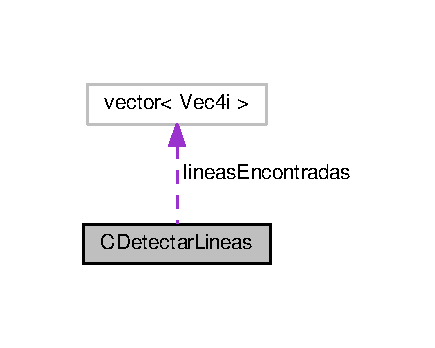
\includegraphics[width=209pt]{classCDetectarLineas__coll__graph}
\end{center}
\end{figure}
\subsection*{Public Member Functions}
\begin{DoxyCompactItemize}
\item 
\hyperlink{classCDetectarLineas_a4a48d20f23a63a2a0202a316317e0801}{C\+Detectar\+Lineas} ()
\begin{DoxyCompactList}\small\item\em Constructor Vacio. \end{DoxyCompactList}\item 
Mat \hyperlink{classCDetectarLineas_a8380e777f5cac60aae54ac0cf13b7246}{iniciar\+Deteccion} (Mat imagen, int houghprobabilistico)
\begin{DoxyCompactList}\small\item\em Metodo que inicia la deteccion de lineas en la imagen. \end{DoxyCompactList}\item 
vector$<$ Vec4i $>$ \& \hyperlink{classCDetectarLineas_ad98f9627f640966b7e11af7d10a4b9e8}{get\+Lineas\+Detectadas} ()
\begin{DoxyCompactList}\small\item\em Metodo que devuelve el conjunto de lineas detectadas en la imagen. \end{DoxyCompactList}\item 
int \hyperlink{classCDetectarLineas_ad7493ac0d73201a7c9188f8a283b6a88}{distancia\+Euclidea} (int a, int b)
\begin{DoxyCompactList}\small\item\em Metodo que devuelve la distancia euclidiana entre dos numeros. \end{DoxyCompactList}\item 
int \hyperlink{classCDetectarLineas_abe5bf1860071f33e7339742fd88e6e78}{distancia\+Euclidea} (int a, int b, bool mostrar)
\begin{DoxyCompactList}\small\item\em Metodo que devuelve la distancia euclidiana entre dos numeros. \end{DoxyCompactList}\item 
int \hyperlink{classCDetectarLineas_a88fe565263283487188f7c032a661d2f}{distancia\+Euclidea} (Point a, Point b)
\begin{DoxyCompactList}\small\item\em Metodo que devuelve la distancia euclidiana entre dos Puntos. \end{DoxyCompactList}\end{DoxyCompactItemize}
\subsection*{Private Member Functions}
\begin{DoxyCompactItemize}
\item 
vector$<$ Vec4i $>$ \hyperlink{classCDetectarLineas_ae70b53c9bf1434cb25e267ea3ab62c63}{detectar\+Lineas} (const Mat \&src\+\_\+gray, int houghprobabilistico)
\begin{DoxyCompactList}\small\item\em Metodo que detecta Lineas en una imagen. \end{DoxyCompactList}\item 
vector$<$ Vec4i $>$ \hyperlink{classCDetectarLineas_ae99dee16338d0e71669d23208e4176de}{Hough\+Probabilistico} (Mat, int, void $\ast$, int houghprobabilistico)
\begin{DoxyCompactList}\small\item\em Metodo para la deteccion de Lineas. \end{DoxyCompactList}\item 
vector$<$ Vec4i $>$ \hyperlink{classCDetectarLineas_a89b7e5edd431909abd180f059f6abd0f}{filtrar\+Lineas} (vector$<$ Vec4i $>$ \&lineas)
\begin{DoxyCompactList}\small\item\em Metodo que filtra lineas extrañas por cercania y duplicidad de principio a fin. \end{DoxyCompactList}\end{DoxyCompactItemize}
\subsection*{Private Attributes}
\begin{DoxyCompactItemize}
\item 
vector$<$ Vec4i $>$ \hyperlink{classCDetectarLineas_a1aab2cfd627e2d3eef1650837ab61436}{lineas\+Encontradas}
\begin{DoxyCompactList}\small\item\em Vector Vec4i de lineas detectadas Estructura x1y1 x2y2. \end{DoxyCompactList}\end{DoxyCompactItemize}


\subsection{Detailed Description}
Clase para la deteccion de Lineas Valor por defecto para la deteccion, hough\+LinesP 80. 

\subsection{Constructor \& Destructor Documentation}
\index{C\+Detectar\+Lineas@{C\+Detectar\+Lineas}!C\+Detectar\+Lineas@{C\+Detectar\+Lineas}}
\index{C\+Detectar\+Lineas@{C\+Detectar\+Lineas}!C\+Detectar\+Lineas@{C\+Detectar\+Lineas}}
\subsubsection[{\texorpdfstring{C\+Detectar\+Lineas()}{CDetectarLineas()}}]{\setlength{\rightskip}{0pt plus 5cm}C\+Detectar\+Lineas\+::\+C\+Detectar\+Lineas (
\begin{DoxyParamCaption}
{}
\end{DoxyParamCaption}
)}\hypertarget{classCDetectarLineas_a4a48d20f23a63a2a0202a316317e0801}{}\label{classCDetectarLineas_a4a48d20f23a63a2a0202a316317e0801}


Constructor Vacio. 



\subsection{Member Function Documentation}
\index{C\+Detectar\+Lineas@{C\+Detectar\+Lineas}!detectar\+Lineas@{detectar\+Lineas}}
\index{detectar\+Lineas@{detectar\+Lineas}!C\+Detectar\+Lineas@{C\+Detectar\+Lineas}}
\subsubsection[{\texorpdfstring{detectar\+Lineas(const Mat \&src\+\_\+gray, int houghprobabilistico)}{detectarLineas(const Mat &src_gray, int houghprobabilistico)}}]{\setlength{\rightskip}{0pt plus 5cm}vector$<$ Vec4i $>$ C\+Detectar\+Lineas\+::detectar\+Lineas (
\begin{DoxyParamCaption}
\item[{const Mat \&}]{src\+\_\+gray, }
\item[{int}]{houghprobabilistico}
\end{DoxyParamCaption}
)\hspace{0.3cm}{\ttfamily [private]}}\hypertarget{classCDetectarLineas_ae70b53c9bf1434cb25e267ea3ab62c63}{}\label{classCDetectarLineas_ae70b53c9bf1434cb25e267ea3ab62c63}


Metodo que detecta Lineas en una imagen. 


\begin{DoxyParams}{Parameters}
{\em src\+\_\+gray.} & Imagen en escala de grises \\
\hline
{\em houghprobabilistico.} & Variable deteccion de lineas. Por defecto 80 \\
\hline
\end{DoxyParams}
\begin{DoxyReturn}{Returns}
Lineas encontradas 
\end{DoxyReturn}
Deteccion de bordes

Deteccion de lineas \index{C\+Detectar\+Lineas@{C\+Detectar\+Lineas}!distancia\+Euclidea@{distancia\+Euclidea}}
\index{distancia\+Euclidea@{distancia\+Euclidea}!C\+Detectar\+Lineas@{C\+Detectar\+Lineas}}
\subsubsection[{\texorpdfstring{distancia\+Euclidea(int a, int b)}{distanciaEuclidea(int a, int b)}}]{\setlength{\rightskip}{0pt plus 5cm}int C\+Detectar\+Lineas\+::distancia\+Euclidea (
\begin{DoxyParamCaption}
\item[{int}]{a, }
\item[{int}]{b}
\end{DoxyParamCaption}
)}\hypertarget{classCDetectarLineas_ad7493ac0d73201a7c9188f8a283b6a88}{}\label{classCDetectarLineas_ad7493ac0d73201a7c9188f8a283b6a88}


Metodo que devuelve la distancia euclidiana entre dos numeros. 


\begin{DoxyParams}{Parameters}
{\em a.} & Numero a \\
\hline
{\em b.} & Numero b \\
\hline
\end{DoxyParams}
\begin{DoxyReturn}{Returns}
distancia euclidiana 
\end{DoxyReturn}
\index{C\+Detectar\+Lineas@{C\+Detectar\+Lineas}!distancia\+Euclidea@{distancia\+Euclidea}}
\index{distancia\+Euclidea@{distancia\+Euclidea}!C\+Detectar\+Lineas@{C\+Detectar\+Lineas}}
\subsubsection[{\texorpdfstring{distancia\+Euclidea(int a, int b, bool mostrar)}{distanciaEuclidea(int a, int b, bool mostrar)}}]{\setlength{\rightskip}{0pt plus 5cm}int C\+Detectar\+Lineas\+::distancia\+Euclidea (
\begin{DoxyParamCaption}
\item[{int}]{a, }
\item[{int}]{b, }
\item[{bool}]{mostrar}
\end{DoxyParamCaption}
)}\hypertarget{classCDetectarLineas_abe5bf1860071f33e7339742fd88e6e78}{}\label{classCDetectarLineas_abe5bf1860071f33e7339742fd88e6e78}


Metodo que devuelve la distancia euclidiana entre dos numeros. 


\begin{DoxyParams}{Parameters}
{\em a.} & Numero a \\
\hline
{\em b.} & Numero b \\
\hline
{\em bool} & mostrar Std resultado \\
\hline
\end{DoxyParams}
\begin{DoxyReturn}{Returns}
distancia euclidiana 
\end{DoxyReturn}
\index{C\+Detectar\+Lineas@{C\+Detectar\+Lineas}!distancia\+Euclidea@{distancia\+Euclidea}}
\index{distancia\+Euclidea@{distancia\+Euclidea}!C\+Detectar\+Lineas@{C\+Detectar\+Lineas}}
\subsubsection[{\texorpdfstring{distancia\+Euclidea(\+Point a, Point b)}{distanciaEuclidea(Point a, Point b)}}]{\setlength{\rightskip}{0pt plus 5cm}int C\+Detectar\+Lineas\+::distancia\+Euclidea (
\begin{DoxyParamCaption}
\item[{Point}]{a, }
\item[{Point}]{b}
\end{DoxyParamCaption}
)}\hypertarget{classCDetectarLineas_a88fe565263283487188f7c032a661d2f}{}\label{classCDetectarLineas_a88fe565263283487188f7c032a661d2f}


Metodo que devuelve la distancia euclidiana entre dos Puntos. 


\begin{DoxyParams}{Parameters}
{\em a.} & Punto a \\
\hline
{\em b.} & Punto b \\
\hline
\end{DoxyParams}
\begin{DoxyReturn}{Returns}
distancia euclidiana 
\end{DoxyReturn}
\index{C\+Detectar\+Lineas@{C\+Detectar\+Lineas}!filtrar\+Lineas@{filtrar\+Lineas}}
\index{filtrar\+Lineas@{filtrar\+Lineas}!C\+Detectar\+Lineas@{C\+Detectar\+Lineas}}
\subsubsection[{\texorpdfstring{filtrar\+Lineas(vector$<$ Vec4i $>$ \&lineas)}{filtrarLineas(vector< Vec4i > &lineas)}}]{\setlength{\rightskip}{0pt plus 5cm}vector$<$ Vec4i $>$ C\+Detectar\+Lineas\+::filtrar\+Lineas (
\begin{DoxyParamCaption}
\item[{vector$<$ Vec4i $>$ \&}]{lineas}
\end{DoxyParamCaption}
)\hspace{0.3cm}{\ttfamily [private]}}\hypertarget{classCDetectarLineas_a89b7e5edd431909abd180f059f6abd0f}{}\label{classCDetectarLineas_a89b7e5edd431909abd180f059f6abd0f}


Metodo que filtra lineas extrañas por cercania y duplicidad de principio a fin. 


\begin{DoxyParams}{Parameters}
{\em lineas} & a filtrar \\
\hline
\end{DoxyParams}
\begin{DoxyReturn}{Returns}
lineas filtradas 
\end{DoxyReturn}
Filtramos la Continuacion de lineas en la coordenada X

continuacion de lineas en Y

Lineas superpuestas completamente, falta las que son sublineas de una mayor \index{C\+Detectar\+Lineas@{C\+Detectar\+Lineas}!get\+Lineas\+Detectadas@{get\+Lineas\+Detectadas}}
\index{get\+Lineas\+Detectadas@{get\+Lineas\+Detectadas}!C\+Detectar\+Lineas@{C\+Detectar\+Lineas}}
\subsubsection[{\texorpdfstring{get\+Lineas\+Detectadas()}{getLineasDetectadas()}}]{\setlength{\rightskip}{0pt plus 5cm}vector$<$ Vec4i $>$ \& C\+Detectar\+Lineas\+::get\+Lineas\+Detectadas (
\begin{DoxyParamCaption}
{}
\end{DoxyParamCaption}
)}\hypertarget{classCDetectarLineas_ad98f9627f640966b7e11af7d10a4b9e8}{}\label{classCDetectarLineas_ad98f9627f640966b7e11af7d10a4b9e8}


Metodo que devuelve el conjunto de lineas detectadas en la imagen. 

\begin{DoxyReturn}{Returns}
vector$<$\+Vec4i$>$ 
\end{DoxyReturn}
\index{C\+Detectar\+Lineas@{C\+Detectar\+Lineas}!Hough\+Probabilistico@{Hough\+Probabilistico}}
\index{Hough\+Probabilistico@{Hough\+Probabilistico}!C\+Detectar\+Lineas@{C\+Detectar\+Lineas}}
\subsubsection[{\texorpdfstring{Hough\+Probabilistico(\+Mat, int, void $\ast$, int houghprobabilistico)}{HoughProbabilistico(Mat, int, void *, int houghprobabilistico)}}]{\setlength{\rightskip}{0pt plus 5cm}vector$<$ Vec4i $>$ C\+Detectar\+Lineas\+::\+Hough\+Probabilistico (
\begin{DoxyParamCaption}
\item[{Mat}]{edges, }
\item[{int}]{, }
\item[{void $\ast$}]{, }
\item[{int}]{houghprobabilistico}
\end{DoxyParamCaption}
)\hspace{0.3cm}{\ttfamily [private]}}\hypertarget{classCDetectarLineas_ae99dee16338d0e71669d23208e4176de}{}\label{classCDetectarLineas_ae99dee16338d0e71669d23208e4176de}


Metodo para la deteccion de Lineas. 


\begin{DoxyParams}{Parameters}
{\em houghprobabilistico.} & Valor variable deteccion de lineas \\
\hline
\end{DoxyParams}
\begin{DoxyReturn}{Returns}

\end{DoxyReturn}
Convertimos la imagen a B\+GR

Usamos la transformada de Hough probabilistica

Filtramos las lineas, duplicaciones \index{C\+Detectar\+Lineas@{C\+Detectar\+Lineas}!iniciar\+Deteccion@{iniciar\+Deteccion}}
\index{iniciar\+Deteccion@{iniciar\+Deteccion}!C\+Detectar\+Lineas@{C\+Detectar\+Lineas}}
\subsubsection[{\texorpdfstring{iniciar\+Deteccion(\+Mat imagen, int houghprobabilistico)}{iniciarDeteccion(Mat imagen, int houghprobabilistico)}}]{\setlength{\rightskip}{0pt plus 5cm}Mat C\+Detectar\+Lineas\+::iniciar\+Deteccion (
\begin{DoxyParamCaption}
\item[{Mat}]{imagen, }
\item[{int}]{houghprobabilistico}
\end{DoxyParamCaption}
)}\hypertarget{classCDetectarLineas_a8380e777f5cac60aae54ac0cf13b7246}{}\label{classCDetectarLineas_a8380e777f5cac60aae54ac0cf13b7246}


Metodo que inicia la deteccion de lineas en la imagen. 


\begin{DoxyParams}{Parameters}
{\em imagen} & \\
\hline
{\em houghprobabilistico.} & Valor de la variable para la deteccion de lineas \\
\hline
\end{DoxyParams}
\begin{DoxyReturn}{Returns}
Imagen resultado de la deteccion 
\end{DoxyReturn}
Deteccion de lineas

Dibujamos lineas sobre la imagen original 

\subsection{Member Data Documentation}
\index{C\+Detectar\+Lineas@{C\+Detectar\+Lineas}!lineas\+Encontradas@{lineas\+Encontradas}}
\index{lineas\+Encontradas@{lineas\+Encontradas}!C\+Detectar\+Lineas@{C\+Detectar\+Lineas}}
\subsubsection[{\texorpdfstring{lineas\+Encontradas}{lineasEncontradas}}]{\setlength{\rightskip}{0pt plus 5cm}vector$<$Vec4i$>$ C\+Detectar\+Lineas\+::lineas\+Encontradas\hspace{0.3cm}{\ttfamily [private]}}\hypertarget{classCDetectarLineas_a1aab2cfd627e2d3eef1650837ab61436}{}\label{classCDetectarLineas_a1aab2cfd627e2d3eef1650837ab61436}


Vector Vec4i de lineas detectadas Estructura x1y1 x2y2. 



The documentation for this class was generated from the following files\+:\begin{DoxyCompactItemize}
\item 
\hyperlink{CDetectarLineas_8h}{C\+Detectar\+Lineas.\+h}\item 
\hyperlink{CDetectarLineas_8cpp}{C\+Detectar\+Lineas.\+cpp}\end{DoxyCompactItemize}

\hypertarget{classCDetectarTransiciones}{}\section{C\+Detectar\+Transiciones Class Reference}
\label{classCDetectarTransiciones}\index{C\+Detectar\+Transiciones@{C\+Detectar\+Transiciones}}


Clase para la dereccion de Transiciones a partir de images.\+xml y classification.\+xml Ambos sacados de Generar\+Clasificador. Proceso de Aprendizaje.  




{\ttfamily \#include $<$C\+Detectar\+Transiciones.\+h$>$}

\subsection*{Public Member Functions}
\begin{DoxyCompactItemize}
\item 
\hyperlink{classCDetectarTransiciones_a99c333a4c8c5a4bb0e03ac09ab6e50b9}{C\+Detectar\+Transiciones} ()
\begin{DoxyCompactList}\small\item\em Constructor Vacio. \end{DoxyCompactList}\item 
bool \hyperlink{classCDetectarTransiciones_a19b374a5d7b5ddb01fada5b3a9d952d7}{ejecutar} (Mat image)
\begin{DoxyCompactList}\small\item\em Metodo que busca las transiciones en una imagen. \end{DoxyCompactList}\item 
Mat \hyperlink{classCDetectarTransiciones_aa9cea5befc08385a46baf86adc305737}{get\+Imagen\+Transicion\+Actual} ()
\begin{DoxyCompactList}\small\item\em Metodo que devuelve la imagen actual. \end{DoxyCompactList}\item 
void \hyperlink{classCDetectarTransiciones_a9f341c8df22490d46b266844b16f8585}{set\+Imagen\+Transicion\+Actual} (Mat image)
\begin{DoxyCompactList}\small\item\em Metodo que asigna una imagen nueva a la imagen a detectar. \end{DoxyCompactList}\item 
vector$<$ \hyperlink{classCContourWithData}{C\+Contour\+With\+Data} $>$ \& \hyperlink{classCDetectarTransiciones_a729c3aaffe2cc888e62c81a58814c1e9}{get\+Contornos\+Encontrados} ()
\begin{DoxyCompactList}\small\item\em Metodo que devuelve los contornos encontrados en la imagen. \end{DoxyCompactList}\item 
vector$<$ char $>$ \& \hyperlink{classCDetectarTransiciones_a1e7c9eac75874737cf7a2b7d7a4375c7}{get\+Letras\+Encontradas} ()
\begin{DoxyCompactList}\small\item\em Metodo que devuelve las letras encontradas en la imagen. Emparejado con los contornos. \end{DoxyCompactList}\end{DoxyCompactItemize}
\subsection*{Private Attributes}
\begin{DoxyCompactItemize}
\item 
Mat \hyperlink{classCDetectarTransiciones_aa58ae70139c85dc3838338eb53a520d3}{imagen\+Transicion\+Actual\+\_\+}
\begin{DoxyCompactList}\small\item\em Imagen actual a detectar Transiciones. \end{DoxyCompactList}\item 
vector$<$ \hyperlink{classCContourWithData}{C\+Contour\+With\+Data} $>$ \hyperlink{classCDetectarTransiciones_a76910f415a085c5e73126ec3fb62a174}{contornos\+Encontrados\+\_\+}
\begin{DoxyCompactList}\small\item\em Vector con los contornos encontrados,. \end{DoxyCompactList}\item 
vector$<$ char $>$ \hyperlink{classCDetectarTransiciones_a0bc5a3fc42f833f3e649e8b8c2fe573d}{letras\+Encontradas\+\_\+}
\begin{DoxyCompactList}\small\item\em Vector con las letras encontradas, emparejado con contorno. \end{DoxyCompactList}\end{DoxyCompactItemize}


\subsection{Detailed Description}
Clase para la dereccion de Transiciones a partir de images.\+xml y classification.\+xml Ambos sacados de Generar\+Clasificador. Proceso de Aprendizaje. 

\subsection{Constructor \& Destructor Documentation}
\index{C\+Detectar\+Transiciones@{C\+Detectar\+Transiciones}!C\+Detectar\+Transiciones@{C\+Detectar\+Transiciones}}
\index{C\+Detectar\+Transiciones@{C\+Detectar\+Transiciones}!C\+Detectar\+Transiciones@{C\+Detectar\+Transiciones}}
\subsubsection[{\texorpdfstring{C\+Detectar\+Transiciones()}{CDetectarTransiciones()}}]{\setlength{\rightskip}{0pt plus 5cm}C\+Detectar\+Transiciones\+::\+C\+Detectar\+Transiciones (
\begin{DoxyParamCaption}
{}
\end{DoxyParamCaption}
)}\hypertarget{classCDetectarTransiciones_a99c333a4c8c5a4bb0e03ac09ab6e50b9}{}\label{classCDetectarTransiciones_a99c333a4c8c5a4bb0e03ac09ab6e50b9}


Constructor Vacio. 



\subsection{Member Function Documentation}
\index{C\+Detectar\+Transiciones@{C\+Detectar\+Transiciones}!ejecutar@{ejecutar}}
\index{ejecutar@{ejecutar}!C\+Detectar\+Transiciones@{C\+Detectar\+Transiciones}}
\subsubsection[{\texorpdfstring{ejecutar(\+Mat image)}{ejecutar(Mat image)}}]{\setlength{\rightskip}{0pt plus 5cm}bool C\+Detectar\+Transiciones\+::ejecutar (
\begin{DoxyParamCaption}
\item[{Mat}]{image}
\end{DoxyParamCaption}
)}\hypertarget{classCDetectarTransiciones_a19b374a5d7b5ddb01fada5b3a9d952d7}{}\label{classCDetectarTransiciones_a19b374a5d7b5ddb01fada5b3a9d952d7}


Metodo que busca las transiciones en una imagen. 


\begin{DoxyParams}{Parameters}
{\em image} & Imagen a detectar \\
\hline
\end{DoxyParams}
\begin{DoxyReturn}{Returns}
Imagen resultado de la deteccion 
\end{DoxyReturn}
Leemos la imagen a detectar, el clasificador.\+xml y image.\+xml

Creamos cv\+::\+Ptr$<$cv\+::ml\+::\+K\+Nearest$>$ k\+Nearest(cv\+::ml\+::\+K\+Nearest\+::create());

instantiate the K\+NN object

Suavizado Gaussiano

Filtro de escala de grises a blanco y negro

Buscamos contornos en la imagen

Ordenamos de izquierda a derecha

k\+Nearest-\/$>$find\+Nearest Buscamos semejanza entre los contornos y el clasificador

Asignamos contorno y letra a contornos\+Encontrados \index{C\+Detectar\+Transiciones@{C\+Detectar\+Transiciones}!get\+Contornos\+Encontrados@{get\+Contornos\+Encontrados}}
\index{get\+Contornos\+Encontrados@{get\+Contornos\+Encontrados}!C\+Detectar\+Transiciones@{C\+Detectar\+Transiciones}}
\subsubsection[{\texorpdfstring{get\+Contornos\+Encontrados()}{getContornosEncontrados()}}]{\setlength{\rightskip}{0pt plus 5cm}vector$<$ {\bf C\+Contour\+With\+Data} $>$ \& C\+Detectar\+Transiciones\+::get\+Contornos\+Encontrados (
\begin{DoxyParamCaption}
{}
\end{DoxyParamCaption}
)}\hypertarget{classCDetectarTransiciones_a729c3aaffe2cc888e62c81a58814c1e9}{}\label{classCDetectarTransiciones_a729c3aaffe2cc888e62c81a58814c1e9}


Metodo que devuelve los contornos encontrados en la imagen. 

\begin{DoxyReturn}{Returns}
vector$<$\+C\+Contour\+With\+Data$>$ 
\end{DoxyReturn}
\index{C\+Detectar\+Transiciones@{C\+Detectar\+Transiciones}!get\+Imagen\+Transicion\+Actual@{get\+Imagen\+Transicion\+Actual}}
\index{get\+Imagen\+Transicion\+Actual@{get\+Imagen\+Transicion\+Actual}!C\+Detectar\+Transiciones@{C\+Detectar\+Transiciones}}
\subsubsection[{\texorpdfstring{get\+Imagen\+Transicion\+Actual()}{getImagenTransicionActual()}}]{\setlength{\rightskip}{0pt plus 5cm}Mat C\+Detectar\+Transiciones\+::get\+Imagen\+Transicion\+Actual (
\begin{DoxyParamCaption}
{}
\end{DoxyParamCaption}
)}\hypertarget{classCDetectarTransiciones_aa9cea5befc08385a46baf86adc305737}{}\label{classCDetectarTransiciones_aa9cea5befc08385a46baf86adc305737}


Metodo que devuelve la imagen actual. 

\begin{DoxyReturn}{Returns}
Mat 
\end{DoxyReturn}
\index{C\+Detectar\+Transiciones@{C\+Detectar\+Transiciones}!get\+Letras\+Encontradas@{get\+Letras\+Encontradas}}
\index{get\+Letras\+Encontradas@{get\+Letras\+Encontradas}!C\+Detectar\+Transiciones@{C\+Detectar\+Transiciones}}
\subsubsection[{\texorpdfstring{get\+Letras\+Encontradas()}{getLetrasEncontradas()}}]{\setlength{\rightskip}{0pt plus 5cm}vector$<$ char $>$ \& C\+Detectar\+Transiciones\+::get\+Letras\+Encontradas (
\begin{DoxyParamCaption}
{}
\end{DoxyParamCaption}
)}\hypertarget{classCDetectarTransiciones_a1e7c9eac75874737cf7a2b7d7a4375c7}{}\label{classCDetectarTransiciones_a1e7c9eac75874737cf7a2b7d7a4375c7}


Metodo que devuelve las letras encontradas en la imagen. Emparejado con los contornos. 

\begin{DoxyReturn}{Returns}
vector$<$\+C\+Contour\+With\+Data$>$ 
\end{DoxyReturn}
\index{C\+Detectar\+Transiciones@{C\+Detectar\+Transiciones}!set\+Imagen\+Transicion\+Actual@{set\+Imagen\+Transicion\+Actual}}
\index{set\+Imagen\+Transicion\+Actual@{set\+Imagen\+Transicion\+Actual}!C\+Detectar\+Transiciones@{C\+Detectar\+Transiciones}}
\subsubsection[{\texorpdfstring{set\+Imagen\+Transicion\+Actual(\+Mat image)}{setImagenTransicionActual(Mat image)}}]{\setlength{\rightskip}{0pt plus 5cm}void C\+Detectar\+Transiciones\+::set\+Imagen\+Transicion\+Actual (
\begin{DoxyParamCaption}
\item[{Mat}]{image}
\end{DoxyParamCaption}
)}\hypertarget{classCDetectarTransiciones_a9f341c8df22490d46b266844b16f8585}{}\label{classCDetectarTransiciones_a9f341c8df22490d46b266844b16f8585}


Metodo que asigna una imagen nueva a la imagen a detectar. 


\begin{DoxyParams}{Parameters}
{\em image.} & Nueva imagen \\
\hline
\end{DoxyParams}


\subsection{Member Data Documentation}
\index{C\+Detectar\+Transiciones@{C\+Detectar\+Transiciones}!contornos\+Encontrados\+\_\+@{contornos\+Encontrados\+\_\+}}
\index{contornos\+Encontrados\+\_\+@{contornos\+Encontrados\+\_\+}!C\+Detectar\+Transiciones@{C\+Detectar\+Transiciones}}
\subsubsection[{\texorpdfstring{contornos\+Encontrados\+\_\+}{contornosEncontrados_}}]{\setlength{\rightskip}{0pt plus 5cm}vector$<${\bf C\+Contour\+With\+Data}$>$ C\+Detectar\+Transiciones\+::contornos\+Encontrados\+\_\+\hspace{0.3cm}{\ttfamily [private]}}\hypertarget{classCDetectarTransiciones_a76910f415a085c5e73126ec3fb62a174}{}\label{classCDetectarTransiciones_a76910f415a085c5e73126ec3fb62a174}


Vector con los contornos encontrados,. 

\index{C\+Detectar\+Transiciones@{C\+Detectar\+Transiciones}!imagen\+Transicion\+Actual\+\_\+@{imagen\+Transicion\+Actual\+\_\+}}
\index{imagen\+Transicion\+Actual\+\_\+@{imagen\+Transicion\+Actual\+\_\+}!C\+Detectar\+Transiciones@{C\+Detectar\+Transiciones}}
\subsubsection[{\texorpdfstring{imagen\+Transicion\+Actual\+\_\+}{imagenTransicionActual_}}]{\setlength{\rightskip}{0pt plus 5cm}Mat C\+Detectar\+Transiciones\+::imagen\+Transicion\+Actual\+\_\+\hspace{0.3cm}{\ttfamily [private]}}\hypertarget{classCDetectarTransiciones_aa58ae70139c85dc3838338eb53a520d3}{}\label{classCDetectarTransiciones_aa58ae70139c85dc3838338eb53a520d3}


Imagen actual a detectar Transiciones. 

\index{C\+Detectar\+Transiciones@{C\+Detectar\+Transiciones}!letras\+Encontradas\+\_\+@{letras\+Encontradas\+\_\+}}
\index{letras\+Encontradas\+\_\+@{letras\+Encontradas\+\_\+}!C\+Detectar\+Transiciones@{C\+Detectar\+Transiciones}}
\subsubsection[{\texorpdfstring{letras\+Encontradas\+\_\+}{letrasEncontradas_}}]{\setlength{\rightskip}{0pt plus 5cm}vector$<$char$>$ C\+Detectar\+Transiciones\+::letras\+Encontradas\+\_\+\hspace{0.3cm}{\ttfamily [private]}}\hypertarget{classCDetectarTransiciones_a0bc5a3fc42f833f3e649e8b8c2fe573d}{}\label{classCDetectarTransiciones_a0bc5a3fc42f833f3e649e8b8c2fe573d}


Vector con las letras encontradas, emparejado con contorno. 



The documentation for this class was generated from the following files\+:\begin{DoxyCompactItemize}
\item 
\hyperlink{CDetectarTransiciones_8h}{C\+Detectar\+Transiciones.\+h}\item 
\hyperlink{CDetectarTransiciones_8cpp}{C\+Detectar\+Transiciones.\+cpp}\end{DoxyCompactItemize}

\hypertarget{classCEstado}{}\section{C\+Estado Class Reference}
\label{classCEstado}\index{C\+Estado@{C\+Estado}}


{\ttfamily \#include $<$C\+Estado\+N\+F\+A.\+h$>$}



Collaboration diagram for C\+Estado\+:
\nopagebreak
\begin{figure}[H]
\begin{center}
\leavevmode
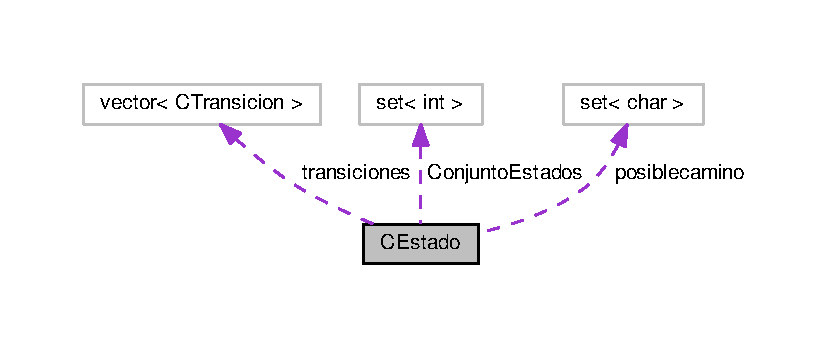
\includegraphics[width=350pt]{classCEstado__coll__graph}
\end{center}
\end{figure}
\subsection*{Public Member Functions}
\begin{DoxyCompactItemize}
\item 
void \hyperlink{classCEstado_a205d938c7acd14b0ec86314162c8813f}{set\+Estado} (bool a, int q, int n\+\_\+trans)
\item 
bool \hyperlink{classCEstado_af1d8101863c51f8d3fca99fc1cd1c883}{get\+Aceptacion} ()
\item 
int \hyperlink{classCEstado_a8578682119ea4b96dbda46cf01db1b28}{get\+\_\+id} ()
\item 
void \hyperlink{classCEstado_a49cb79111fb7daa925857e8e38ca8c6b}{set\+\_\+id} (int i)
\item 
bool \hyperlink{classCEstado_aeb0a7a2c71a2c26471ddbc851c907f50}{get\+Muerte} ()
\item 
void \hyperlink{classCEstado_a010660248a8521d9df60d6e1d81ab92b}{Mostrar\+N\+FA} ()
\item 
void \hyperlink{classCEstado_ad08f6f204f257fb7e12436bbcc40b0f4}{insertar\+\_\+transicion} (\hyperlink{classCTransicion}{C\+Transicion} tran)
\item 
\hyperlink{classCTransicion}{C\+Transicion} \hyperlink{classCEstado_a307188d33798e78407233d65860f852d}{get\+\_\+transicion} (int i)
\item 
int \hyperlink{classCEstado_a412cdf24853e656329b64ef239e1ba2e}{get\+\_\+n\+\_\+trans} ()
\item 
void \hyperlink{classCEstado_adf87b55f9d93e237e768345ac34ba62d}{set\+\_\+muerte} (bool p)
\item 
void \hyperlink{classCEstado_aa7759717e41bb25d7ee5c5fff99dde87}{set\+\_\+aceptacion} (bool p)
\item 
bool \hyperlink{classCEstado_ace37ed71a9ddc500a3ce577b9f19ee85}{existecamino} (char variable)
\item 
void \hyperlink{classCEstado_a9b47f1bd5bb83afc3902c888aa4d346d}{insertar\+\_\+estado} (int \hyperlink{classCEstado_a2ff2cdec56804f70b389076be4501b4c}{q\+\_\+id})
\item 
set$<$ int $>$ \hyperlink{classCEstado_aa2f32f993b57466e5ba33bc82e52b60d}{Retornar\+Conjunto} ()
\end{DoxyCompactItemize}
\subsection*{Private Attributes}
\begin{DoxyCompactItemize}
\item 
bool \hyperlink{classCEstado_a1388d38c2984906e8f773cc1227d99b2}{aceptacion}
\item 
int \hyperlink{classCEstado_a2ff2cdec56804f70b389076be4501b4c}{q\+\_\+id}
\item 
bool \hyperlink{classCEstado_a2ff59531bf70a06d0a895eea962553e4}{muerte}
\item 
int \hyperlink{classCEstado_a9e66500a59a8b5437f3a89a79e91d472}{n\+\_\+transiciones}
\item 
vector$<$ \hyperlink{classCTransicion}{C\+Transicion} $>$ \hyperlink{classCEstado_a5f904405b10b0826dd1749fdb9c6f302}{transiciones}
\item 
set$<$ char $>$ \hyperlink{classCEstado_ac7e32bb24d14ad8f5b2d23e273087bd0}{posiblecamino}
\item 
set$<$ int $>$ \hyperlink{classCEstado_a28265d36807fa3c84140e23872fb0132}{Conjunto\+Estados}
\end{DoxyCompactItemize}


\subsection{Member Function Documentation}
\index{C\+Estado@{C\+Estado}!existecamino@{existecamino}}
\index{existecamino@{existecamino}!C\+Estado@{C\+Estado}}
\subsubsection[{\texorpdfstring{existecamino(char variable)}{existecamino(char variable)}}]{\setlength{\rightskip}{0pt plus 5cm}bool C\+Estado\+::existecamino (
\begin{DoxyParamCaption}
\item[{char}]{variable}
\end{DoxyParamCaption}
)}\hypertarget{classCEstado_ace37ed71a9ddc500a3ce577b9f19ee85}{}\label{classCEstado_ace37ed71a9ddc500a3ce577b9f19ee85}
\index{C\+Estado@{C\+Estado}!get\+\_\+id@{get\+\_\+id}}
\index{get\+\_\+id@{get\+\_\+id}!C\+Estado@{C\+Estado}}
\subsubsection[{\texorpdfstring{get\+\_\+id()}{get_id()}}]{\setlength{\rightskip}{0pt plus 5cm}int C\+Estado\+::get\+\_\+id (
\begin{DoxyParamCaption}
{}
\end{DoxyParamCaption}
)}\hypertarget{classCEstado_a8578682119ea4b96dbda46cf01db1b28}{}\label{classCEstado_a8578682119ea4b96dbda46cf01db1b28}
\index{C\+Estado@{C\+Estado}!get\+\_\+n\+\_\+trans@{get\+\_\+n\+\_\+trans}}
\index{get\+\_\+n\+\_\+trans@{get\+\_\+n\+\_\+trans}!C\+Estado@{C\+Estado}}
\subsubsection[{\texorpdfstring{get\+\_\+n\+\_\+trans()}{get_n_trans()}}]{\setlength{\rightskip}{0pt plus 5cm}int C\+Estado\+::get\+\_\+n\+\_\+trans (
\begin{DoxyParamCaption}
{}
\end{DoxyParamCaption}
)}\hypertarget{classCEstado_a412cdf24853e656329b64ef239e1ba2e}{}\label{classCEstado_a412cdf24853e656329b64ef239e1ba2e}
\index{C\+Estado@{C\+Estado}!get\+\_\+transicion@{get\+\_\+transicion}}
\index{get\+\_\+transicion@{get\+\_\+transicion}!C\+Estado@{C\+Estado}}
\subsubsection[{\texorpdfstring{get\+\_\+transicion(int i)}{get_transicion(int i)}}]{\setlength{\rightskip}{0pt plus 5cm}{\bf C\+Transicion} C\+Estado\+::get\+\_\+transicion (
\begin{DoxyParamCaption}
\item[{int}]{i}
\end{DoxyParamCaption}
)}\hypertarget{classCEstado_a307188d33798e78407233d65860f852d}{}\label{classCEstado_a307188d33798e78407233d65860f852d}
\index{C\+Estado@{C\+Estado}!get\+Aceptacion@{get\+Aceptacion}}
\index{get\+Aceptacion@{get\+Aceptacion}!C\+Estado@{C\+Estado}}
\subsubsection[{\texorpdfstring{get\+Aceptacion()}{getAceptacion()}}]{\setlength{\rightskip}{0pt plus 5cm}bool C\+Estado\+::get\+Aceptacion (
\begin{DoxyParamCaption}
{}
\end{DoxyParamCaption}
)}\hypertarget{classCEstado_af1d8101863c51f8d3fca99fc1cd1c883}{}\label{classCEstado_af1d8101863c51f8d3fca99fc1cd1c883}
\index{C\+Estado@{C\+Estado}!get\+Muerte@{get\+Muerte}}
\index{get\+Muerte@{get\+Muerte}!C\+Estado@{C\+Estado}}
\subsubsection[{\texorpdfstring{get\+Muerte()}{getMuerte()}}]{\setlength{\rightskip}{0pt plus 5cm}bool C\+Estado\+::get\+Muerte (
\begin{DoxyParamCaption}
{}
\end{DoxyParamCaption}
)}\hypertarget{classCEstado_aeb0a7a2c71a2c26471ddbc851c907f50}{}\label{classCEstado_aeb0a7a2c71a2c26471ddbc851c907f50}
\index{C\+Estado@{C\+Estado}!insertar\+\_\+estado@{insertar\+\_\+estado}}
\index{insertar\+\_\+estado@{insertar\+\_\+estado}!C\+Estado@{C\+Estado}}
\subsubsection[{\texorpdfstring{insertar\+\_\+estado(int q\+\_\+id)}{insertar_estado(int q_id)}}]{\setlength{\rightskip}{0pt plus 5cm}void C\+Estado\+::insertar\+\_\+estado (
\begin{DoxyParamCaption}
\item[{int}]{q\+\_\+id}
\end{DoxyParamCaption}
)}\hypertarget{classCEstado_a9b47f1bd5bb83afc3902c888aa4d346d}{}\label{classCEstado_a9b47f1bd5bb83afc3902c888aa4d346d}
\index{C\+Estado@{C\+Estado}!insertar\+\_\+transicion@{insertar\+\_\+transicion}}
\index{insertar\+\_\+transicion@{insertar\+\_\+transicion}!C\+Estado@{C\+Estado}}
\subsubsection[{\texorpdfstring{insertar\+\_\+transicion(\+C\+Transicion tran)}{insertar_transicion(CTransicion tran)}}]{\setlength{\rightskip}{0pt plus 5cm}void C\+Estado\+::insertar\+\_\+transicion (
\begin{DoxyParamCaption}
\item[{{\bf C\+Transicion}}]{tran}
\end{DoxyParamCaption}
)}\hypertarget{classCEstado_ad08f6f204f257fb7e12436bbcc40b0f4}{}\label{classCEstado_ad08f6f204f257fb7e12436bbcc40b0f4}
\index{C\+Estado@{C\+Estado}!Mostrar\+N\+FA@{Mostrar\+N\+FA}}
\index{Mostrar\+N\+FA@{Mostrar\+N\+FA}!C\+Estado@{C\+Estado}}
\subsubsection[{\texorpdfstring{Mostrar\+N\+F\+A()}{MostrarNFA()}}]{\setlength{\rightskip}{0pt plus 5cm}void C\+Estado\+::\+Mostrar\+N\+FA (
\begin{DoxyParamCaption}
{}
\end{DoxyParamCaption}
)}\hypertarget{classCEstado_a010660248a8521d9df60d6e1d81ab92b}{}\label{classCEstado_a010660248a8521d9df60d6e1d81ab92b}
\index{C\+Estado@{C\+Estado}!Retornar\+Conjunto@{Retornar\+Conjunto}}
\index{Retornar\+Conjunto@{Retornar\+Conjunto}!C\+Estado@{C\+Estado}}
\subsubsection[{\texorpdfstring{Retornar\+Conjunto()}{RetornarConjunto()}}]{\setlength{\rightskip}{0pt plus 5cm}set$<$ int $>$ C\+Estado\+::\+Retornar\+Conjunto (
\begin{DoxyParamCaption}
{}
\end{DoxyParamCaption}
)}\hypertarget{classCEstado_aa2f32f993b57466e5ba33bc82e52b60d}{}\label{classCEstado_aa2f32f993b57466e5ba33bc82e52b60d}
\index{C\+Estado@{C\+Estado}!set\+\_\+aceptacion@{set\+\_\+aceptacion}}
\index{set\+\_\+aceptacion@{set\+\_\+aceptacion}!C\+Estado@{C\+Estado}}
\subsubsection[{\texorpdfstring{set\+\_\+aceptacion(bool p)}{set_aceptacion(bool p)}}]{\setlength{\rightskip}{0pt plus 5cm}void C\+Estado\+::set\+\_\+aceptacion (
\begin{DoxyParamCaption}
\item[{bool}]{p}
\end{DoxyParamCaption}
)}\hypertarget{classCEstado_aa7759717e41bb25d7ee5c5fff99dde87}{}\label{classCEstado_aa7759717e41bb25d7ee5c5fff99dde87}
\index{C\+Estado@{C\+Estado}!set\+\_\+id@{set\+\_\+id}}
\index{set\+\_\+id@{set\+\_\+id}!C\+Estado@{C\+Estado}}
\subsubsection[{\texorpdfstring{set\+\_\+id(int i)}{set_id(int i)}}]{\setlength{\rightskip}{0pt plus 5cm}void C\+Estado\+::set\+\_\+id (
\begin{DoxyParamCaption}
\item[{int}]{i}
\end{DoxyParamCaption}
)}\hypertarget{classCEstado_a49cb79111fb7daa925857e8e38ca8c6b}{}\label{classCEstado_a49cb79111fb7daa925857e8e38ca8c6b}
\index{C\+Estado@{C\+Estado}!set\+\_\+muerte@{set\+\_\+muerte}}
\index{set\+\_\+muerte@{set\+\_\+muerte}!C\+Estado@{C\+Estado}}
\subsubsection[{\texorpdfstring{set\+\_\+muerte(bool p)}{set_muerte(bool p)}}]{\setlength{\rightskip}{0pt plus 5cm}void C\+Estado\+::set\+\_\+muerte (
\begin{DoxyParamCaption}
\item[{bool}]{p}
\end{DoxyParamCaption}
)}\hypertarget{classCEstado_adf87b55f9d93e237e768345ac34ba62d}{}\label{classCEstado_adf87b55f9d93e237e768345ac34ba62d}
\index{C\+Estado@{C\+Estado}!set\+Estado@{set\+Estado}}
\index{set\+Estado@{set\+Estado}!C\+Estado@{C\+Estado}}
\subsubsection[{\texorpdfstring{set\+Estado(bool a, int q, int n\+\_\+trans)}{setEstado(bool a, int q, int n_trans)}}]{\setlength{\rightskip}{0pt plus 5cm}void C\+Estado\+::set\+Estado (
\begin{DoxyParamCaption}
\item[{bool}]{a, }
\item[{int}]{q, }
\item[{int}]{n\+\_\+trans}
\end{DoxyParamCaption}
)}\hypertarget{classCEstado_a205d938c7acd14b0ec86314162c8813f}{}\label{classCEstado_a205d938c7acd14b0ec86314162c8813f}


\subsection{Member Data Documentation}
\index{C\+Estado@{C\+Estado}!aceptacion@{aceptacion}}
\index{aceptacion@{aceptacion}!C\+Estado@{C\+Estado}}
\subsubsection[{\texorpdfstring{aceptacion}{aceptacion}}]{\setlength{\rightskip}{0pt plus 5cm}bool C\+Estado\+::aceptacion\hspace{0.3cm}{\ttfamily [private]}}\hypertarget{classCEstado_a1388d38c2984906e8f773cc1227d99b2}{}\label{classCEstado_a1388d38c2984906e8f773cc1227d99b2}
\index{C\+Estado@{C\+Estado}!Conjunto\+Estados@{Conjunto\+Estados}}
\index{Conjunto\+Estados@{Conjunto\+Estados}!C\+Estado@{C\+Estado}}
\subsubsection[{\texorpdfstring{Conjunto\+Estados}{ConjuntoEstados}}]{\setlength{\rightskip}{0pt plus 5cm}set$<$int$>$ C\+Estado\+::\+Conjunto\+Estados\hspace{0.3cm}{\ttfamily [private]}}\hypertarget{classCEstado_a28265d36807fa3c84140e23872fb0132}{}\label{classCEstado_a28265d36807fa3c84140e23872fb0132}
\index{C\+Estado@{C\+Estado}!muerte@{muerte}}
\index{muerte@{muerte}!C\+Estado@{C\+Estado}}
\subsubsection[{\texorpdfstring{muerte}{muerte}}]{\setlength{\rightskip}{0pt plus 5cm}bool C\+Estado\+::muerte\hspace{0.3cm}{\ttfamily [private]}}\hypertarget{classCEstado_a2ff59531bf70a06d0a895eea962553e4}{}\label{classCEstado_a2ff59531bf70a06d0a895eea962553e4}
\index{C\+Estado@{C\+Estado}!n\+\_\+transiciones@{n\+\_\+transiciones}}
\index{n\+\_\+transiciones@{n\+\_\+transiciones}!C\+Estado@{C\+Estado}}
\subsubsection[{\texorpdfstring{n\+\_\+transiciones}{n_transiciones}}]{\setlength{\rightskip}{0pt plus 5cm}int C\+Estado\+::n\+\_\+transiciones\hspace{0.3cm}{\ttfamily [private]}}\hypertarget{classCEstado_a9e66500a59a8b5437f3a89a79e91d472}{}\label{classCEstado_a9e66500a59a8b5437f3a89a79e91d472}
\index{C\+Estado@{C\+Estado}!posiblecamino@{posiblecamino}}
\index{posiblecamino@{posiblecamino}!C\+Estado@{C\+Estado}}
\subsubsection[{\texorpdfstring{posiblecamino}{posiblecamino}}]{\setlength{\rightskip}{0pt plus 5cm}set$<$char$>$ C\+Estado\+::posiblecamino\hspace{0.3cm}{\ttfamily [private]}}\hypertarget{classCEstado_ac7e32bb24d14ad8f5b2d23e273087bd0}{}\label{classCEstado_ac7e32bb24d14ad8f5b2d23e273087bd0}
\index{C\+Estado@{C\+Estado}!q\+\_\+id@{q\+\_\+id}}
\index{q\+\_\+id@{q\+\_\+id}!C\+Estado@{C\+Estado}}
\subsubsection[{\texorpdfstring{q\+\_\+id}{q_id}}]{\setlength{\rightskip}{0pt plus 5cm}int C\+Estado\+::q\+\_\+id\hspace{0.3cm}{\ttfamily [private]}}\hypertarget{classCEstado_a2ff2cdec56804f70b389076be4501b4c}{}\label{classCEstado_a2ff2cdec56804f70b389076be4501b4c}
\index{C\+Estado@{C\+Estado}!transiciones@{transiciones}}
\index{transiciones@{transiciones}!C\+Estado@{C\+Estado}}
\subsubsection[{\texorpdfstring{transiciones}{transiciones}}]{\setlength{\rightskip}{0pt plus 5cm}vector$<${\bf C\+Transicion}$>$ C\+Estado\+::transiciones\hspace{0.3cm}{\ttfamily [private]}}\hypertarget{classCEstado_a5f904405b10b0826dd1749fdb9c6f302}{}\label{classCEstado_a5f904405b10b0826dd1749fdb9c6f302}


The documentation for this class was generated from the following files\+:\begin{DoxyCompactItemize}
\item 
\hyperlink{CEstadoNFA_8h}{C\+Estado\+N\+F\+A.\+h}\item 
\hyperlink{CEstadoNFA_8cpp}{C\+Estado\+N\+F\+A.\+cpp}\end{DoxyCompactItemize}

\hypertarget{classCFiltrosImagenes}{}\section{C\+Filtros\+Imagenes Class Reference}
\label{classCFiltrosImagenes}\index{C\+Filtros\+Imagenes@{C\+Filtros\+Imagenes}}


{\ttfamily \#include $<$C\+Filtros\+Imagenes.\+h$>$}

\subsection*{Public Member Functions}
\begin{DoxyCompactItemize}
\item 
\hyperlink{classCFiltrosImagenes_a6478e212e79b6c075c13f92fd8a500e2}{C\+Filtros\+Imagenes} ()
\item 
Mat \hyperlink{classCFiltrosImagenes_a4fb22fba45bab47d81904429e8f250f0}{filtro\+Gaussian\+Blur} (Mat original)
\item 
Mat \hyperlink{classCFiltrosImagenes_a98ef01d019a234d186e1ac47d76c09de}{filtro\+Median\+Blur} (Mat original)
\item 
Mat \hyperlink{classCFiltrosImagenes_a6ba12449903681d11aba15c065e48e61}{filtro\+Sobel} (Mat original)
\item 
Mat \hyperlink{classCFiltrosImagenes_ad9cd3070a534acc987a3bf15555590c2}{filtro\+Laplacian} (Mat original)
\item 
void \hyperlink{classCFiltrosImagenes_ac5bf9185d05955f93480cba9f158641d}{prueba\+Filtros} ()
\end{DoxyCompactItemize}


\subsection{Constructor \& Destructor Documentation}
\index{C\+Filtros\+Imagenes@{C\+Filtros\+Imagenes}!C\+Filtros\+Imagenes@{C\+Filtros\+Imagenes}}
\index{C\+Filtros\+Imagenes@{C\+Filtros\+Imagenes}!C\+Filtros\+Imagenes@{C\+Filtros\+Imagenes}}
\subsubsection[{\texorpdfstring{C\+Filtros\+Imagenes()}{CFiltrosImagenes()}}]{\setlength{\rightskip}{0pt plus 5cm}C\+Filtros\+Imagenes\+::\+C\+Filtros\+Imagenes (
\begin{DoxyParamCaption}
{}
\end{DoxyParamCaption}
)}\hypertarget{classCFiltrosImagenes_a6478e212e79b6c075c13f92fd8a500e2}{}\label{classCFiltrosImagenes_a6478e212e79b6c075c13f92fd8a500e2}


\subsection{Member Function Documentation}
\index{C\+Filtros\+Imagenes@{C\+Filtros\+Imagenes}!filtro\+Gaussian\+Blur@{filtro\+Gaussian\+Blur}}
\index{filtro\+Gaussian\+Blur@{filtro\+Gaussian\+Blur}!C\+Filtros\+Imagenes@{C\+Filtros\+Imagenes}}
\subsubsection[{\texorpdfstring{filtro\+Gaussian\+Blur(\+Mat original)}{filtroGaussianBlur(Mat original)}}]{\setlength{\rightskip}{0pt plus 5cm}Mat C\+Filtros\+Imagenes\+::filtro\+Gaussian\+Blur (
\begin{DoxyParamCaption}
\item[{Mat}]{original}
\end{DoxyParamCaption}
)}\hypertarget{classCFiltrosImagenes_a4fb22fba45bab47d81904429e8f250f0}{}\label{classCFiltrosImagenes_a4fb22fba45bab47d81904429e8f250f0}
\index{C\+Filtros\+Imagenes@{C\+Filtros\+Imagenes}!filtro\+Laplacian@{filtro\+Laplacian}}
\index{filtro\+Laplacian@{filtro\+Laplacian}!C\+Filtros\+Imagenes@{C\+Filtros\+Imagenes}}
\subsubsection[{\texorpdfstring{filtro\+Laplacian(\+Mat original)}{filtroLaplacian(Mat original)}}]{\setlength{\rightskip}{0pt plus 5cm}Mat C\+Filtros\+Imagenes\+::filtro\+Laplacian (
\begin{DoxyParamCaption}
\item[{Mat}]{original}
\end{DoxyParamCaption}
)}\hypertarget{classCFiltrosImagenes_ad9cd3070a534acc987a3bf15555590c2}{}\label{classCFiltrosImagenes_ad9cd3070a534acc987a3bf15555590c2}
\index{C\+Filtros\+Imagenes@{C\+Filtros\+Imagenes}!filtro\+Median\+Blur@{filtro\+Median\+Blur}}
\index{filtro\+Median\+Blur@{filtro\+Median\+Blur}!C\+Filtros\+Imagenes@{C\+Filtros\+Imagenes}}
\subsubsection[{\texorpdfstring{filtro\+Median\+Blur(\+Mat original)}{filtroMedianBlur(Mat original)}}]{\setlength{\rightskip}{0pt plus 5cm}Mat C\+Filtros\+Imagenes\+::filtro\+Median\+Blur (
\begin{DoxyParamCaption}
\item[{Mat}]{original}
\end{DoxyParamCaption}
)}\hypertarget{classCFiltrosImagenes_a98ef01d019a234d186e1ac47d76c09de}{}\label{classCFiltrosImagenes_a98ef01d019a234d186e1ac47d76c09de}
\index{C\+Filtros\+Imagenes@{C\+Filtros\+Imagenes}!filtro\+Sobel@{filtro\+Sobel}}
\index{filtro\+Sobel@{filtro\+Sobel}!C\+Filtros\+Imagenes@{C\+Filtros\+Imagenes}}
\subsubsection[{\texorpdfstring{filtro\+Sobel(\+Mat original)}{filtroSobel(Mat original)}}]{\setlength{\rightskip}{0pt plus 5cm}Mat C\+Filtros\+Imagenes\+::filtro\+Sobel (
\begin{DoxyParamCaption}
\item[{Mat}]{original}
\end{DoxyParamCaption}
)}\hypertarget{classCFiltrosImagenes_a6ba12449903681d11aba15c065e48e61}{}\label{classCFiltrosImagenes_a6ba12449903681d11aba15c065e48e61}
\index{C\+Filtros\+Imagenes@{C\+Filtros\+Imagenes}!prueba\+Filtros@{prueba\+Filtros}}
\index{prueba\+Filtros@{prueba\+Filtros}!C\+Filtros\+Imagenes@{C\+Filtros\+Imagenes}}
\subsubsection[{\texorpdfstring{prueba\+Filtros()}{pruebaFiltros()}}]{\setlength{\rightskip}{0pt plus 5cm}void C\+Filtros\+Imagenes\+::prueba\+Filtros (
\begin{DoxyParamCaption}
{}
\end{DoxyParamCaption}
)}\hypertarget{classCFiltrosImagenes_ac5bf9185d05955f93480cba9f158641d}{}\label{classCFiltrosImagenes_ac5bf9185d05955f93480cba9f158641d}


The documentation for this class was generated from the following files\+:\begin{DoxyCompactItemize}
\item 
\hyperlink{CFiltrosImagenes_8h}{C\+Filtros\+Imagenes.\+h}\item 
\hyperlink{CFiltrosImagenes_8cpp}{C\+Filtros\+Imagenes.\+cpp}\end{DoxyCompactItemize}

\hypertarget{classCLabel}{}\section{C\+Label Class Reference}
\label{classCLabel}\index{C\+Label@{C\+Label}}


Inheritance diagram for C\+Label\+:
% FIG 0


Collaboration diagram for C\+Label\+:
% FIG 1
\subsection*{Public Member Functions}
\begin{DoxyCompactItemize}
\item 
{\bfseries C\+Label} (Q\+String text, bool)\hypertarget{classCLabel_a6e88fa51b6c55ae59b71498cdba66ea8}{}\label{classCLabel_a6e88fa51b6c55ae59b71498cdba66ea8}

\item 
Q\+Image {\bfseries get\+Imagen} ()\hypertarget{classCLabel_a79ebc8b728db45da16020cdeb2439625}{}\label{classCLabel_a79ebc8b728db45da16020cdeb2439625}

\item 
void {\bfseries set\+Imagen} (const Q\+Image)\hypertarget{classCLabel_ac44138a6205fa3b2bc8eee63263e6fc7}{}\label{classCLabel_ac44138a6205fa3b2bc8eee63263e6fc7}

\end{DoxyCompactItemize}


The documentation for this class was generated from the following files\+:\begin{DoxyCompactItemize}
\item 
C\+Label.\+h\item 
C\+Label.\+cpp\end{DoxyCompactItemize}

\hypertarget{classCLineEdit}{}\section{C\+Line\+Edit Class Reference}
\label{classCLineEdit}\index{C\+Line\+Edit@{C\+Line\+Edit}}


{\ttfamily \#include $<$C\+Line\+Edit.\+h$>$}



Inheritance diagram for C\+Line\+Edit\+:
% FIG 0


Collaboration diagram for C\+Line\+Edit\+:
% FIG 1
\subsection*{Public Member Functions}
\begin{DoxyCompactItemize}
\item 
\hyperlink{classCLineEdit_afb3493949a61a9d51eea5182bfc0a591}{C\+Line\+Edit} ()\hypertarget{classCLineEdit_afb3493949a61a9d51eea5182bfc0a591}{}\label{classCLineEdit_afb3493949a61a9d51eea5182bfc0a591}

\begin{DoxyCompactList}\small\item\em \hyperlink{classCLineEdit}{C\+Line\+Edit} Constructor con estilo centrado y fondo blanco. \end{DoxyCompactList}\item 
\hyperlink{classCLineEdit_a67d172f77a4cd9233aee3684248436f5}{C\+Line\+Edit} (Q\+String text)
\begin{DoxyCompactList}\small\item\em \hyperlink{classCLineEdit}{C\+Line\+Edit}. \end{DoxyCompactList}\item 
\hyperlink{classCLineEdit_a4d03efd8b636f5f9a584200e222ca6cc}{$\sim$\+C\+Line\+Edit} ()\hypertarget{classCLineEdit_a4d03efd8b636f5f9a584200e222ca6cc}{}\label{classCLineEdit_a4d03efd8b636f5f9a584200e222ca6cc}

\begin{DoxyCompactList}\small\item\em Destructor. \end{DoxyCompactList}\end{DoxyCompactItemize}


\subsection{Detailed Description}
Clase heredada de \textquotesingle{}Q\+Line\+Edit\textquotesingle{} que aplica un estilo determinado a este tipo de container 

\subsection{Constructor \& Destructor Documentation}
\index{C\+Line\+Edit@{C\+Line\+Edit}!C\+Line\+Edit@{C\+Line\+Edit}}
\index{C\+Line\+Edit@{C\+Line\+Edit}!C\+Line\+Edit@{C\+Line\+Edit}}
\subsubsection[{\texorpdfstring{C\+Line\+Edit(\+Q\+String text)}{CLineEdit(QString text)}}]{\setlength{\rightskip}{0pt plus 5cm}C\+Line\+Edit\+::\+C\+Line\+Edit (
\begin{DoxyParamCaption}
\item[{Q\+String}]{text}
\end{DoxyParamCaption}
)}\hypertarget{classCLineEdit_a67d172f77a4cd9233aee3684248436f5}{}\label{classCLineEdit_a67d172f77a4cd9233aee3684248436f5}


\hyperlink{classCLineEdit}{C\+Line\+Edit}. 


\begin{DoxyParams}{Parameters}
{\em text} & Texto a introducir en el Q\+Line\+Edit \\
\hline
\end{DoxyParams}


The documentation for this class was generated from the following files\+:\begin{DoxyCompactItemize}
\item 
C\+Line\+Edit.\+h\item 
C\+Line\+Edit.\+cpp\end{DoxyCompactItemize}

\hypertarget{classCNFA}{}\section{C\+N\+FA Class Reference}
\label{classCNFA}\index{C\+N\+FA@{C\+N\+FA}}


{\ttfamily \#include $<$C\+Nfa.\+h$>$}



Collaboration diagram for C\+N\+FA\+:
\nopagebreak
\begin{figure}[H]
\begin{center}
\leavevmode
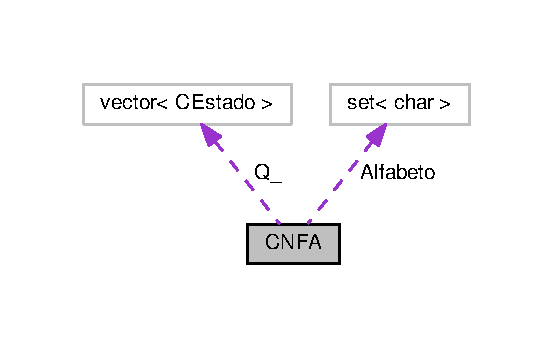
\includegraphics[width=266pt]{classCNFA__coll__graph}
\end{center}
\end{figure}
\subsection*{Public Member Functions}
\begin{DoxyCompactItemize}
\item 
\hyperlink{classCEstado}{C\+Estado} \hyperlink{classCNFA_adefa2ccc519fcc5776f22b52ab7896a5}{encontrar\+Estado} (int q\+\_\+id)
\item 
void \hyperlink{classCNFA_ada66fe5bfcef0f2029d919fce2b7a101}{Construir\+N\+FA} (Q\+String nombrefichero)
\item 
string \hyperlink{classCNFA_a2229a8054ba76749dbeb90c20e4ed43b}{Mostrar\+Estados\+Muerte} ()
\item 
void \hyperlink{classCNFA_a856bedb1c7ed1b4e12bd9e3169de6831}{Mostrar\+N\+FA} ()
\item 
bool \hyperlink{classCNFA_a7ddf2ec61f8b50ca52835f9cef329df2}{Analizar} (\hyperlink{classCEstado}{C\+Estado} \&q, string \&cadena, int t, vector$<$ \hyperlink{classCTransicion}{C\+Transicion} $>$ \&caminos, bool \&acepta)
\item 
string \hyperlink{classCNFA_a9fee58c888ab16ea8e87bfbecd5252c8}{Analizar\+Cadena} (string \&cadena)
\item 
void \hyperlink{classCNFA_ae54534591a2ab8f762c95bcd2e8b3bdd}{Mostrar\+Camino} (vector$<$ \hyperlink{classCTransicion}{C\+Transicion} $>$ \&Camino)
\item 
void \hyperlink{classCNFA_ab5b7d6d69a73fea0eaa37f77b7c976d3}{Crear\+Alfabeto} ()
\item 
string \hyperlink{classCNFA_af87caa9992ea843c0252977bc150f382}{Mostrar\+Alfabeto} ()
\item 
void \hyperlink{classCNFA_ab44a10890c442fa25b505d4d4c1893f3}{epsilon\+Closure} (\hyperlink{classCEstado}{C\+Estado} \&q, \hyperlink{classCEstado}{C\+Estado} \&A)
\item 
void \hyperlink{classCNFA_ab267d2860617072d1ade5a6021baf07c}{epsilon\+Closure} (\hyperlink{classCEstado}{C\+Estado} \&A)
\item 
\hyperlink{classCEstado}{C\+Estado} \hyperlink{classCNFA_a4dc5f0d4dd40d4f160c1ad36d13dfb28}{move} (set$<$ int $>$ \&A, char simbolo)
\item 
int \hyperlink{classCNFA_a736e324e3fb34554aa260850d1f00980}{Encontrarpos} (\hyperlink{classCEstado}{C\+Estado} \&A, vector$<$ \hyperlink{classCEstado}{C\+Estado} $>$ \&Orden)
\item 
bool \hyperlink{classCNFA_a15d5ce134bcb51243b301a8817af83ab}{Existe} (\hyperlink{classCEstado}{C\+Estado} \&A, vector$<$ \hyperlink{classCEstado}{C\+Estado} $>$ \&Orden)
\item 
vector$<$ \hyperlink{classCEstado}{C\+Estado} $>$ \hyperlink{classCNFA_a98d4f959c5cfc04a02863bf8f23d295e}{Convertto\+D\+FA} ()
\item 
bool \hyperlink{classCNFA_ae8331e19d188fbf2a0702d79860ac21b}{igualdad} (set$<$ int $>$ \&A, set$<$ int $>$ \&B)
\item 
void \hyperlink{classCNFA_a09aebebe74a38efbbcc5b2f5b1f6972e}{aceptacion\+\_\+id} (vector$<$ \hyperlink{classCEstado}{C\+Estado} $>$ \&Orden)
\item 
void \hyperlink{classCNFA_a78f025cb7fcf04abdc659fa6c9075667}{Exportar} (vector$<$ \hyperlink{classCEstado}{C\+Estado} $>$ \&Orden)
\end{DoxyCompactItemize}
\subsection*{Private Attributes}
\begin{DoxyCompactItemize}
\item 
vector$<$ \hyperlink{classCEstado}{C\+Estado} $>$ \hyperlink{classCNFA_a28a2f71306cb27d725bad4093c5c82c7}{Q\+\_\+}
\item 
int \hyperlink{classCNFA_af402d09515afcb02ba12c4a0c762aac8}{inicial}
\item 
int \hyperlink{classCNFA_a887785fdfe01da854067ca5b528da79c}{n\+\_\+estados}
\item 
set$<$ char $>$ \hyperlink{classCNFA_af7972ada0c1a2d1eecde53fb4f47bb2a}{Alfabeto}
\end{DoxyCompactItemize}


\subsection{Member Function Documentation}
\index{C\+N\+FA@{C\+N\+FA}!aceptacion\+\_\+id@{aceptacion\+\_\+id}}
\index{aceptacion\+\_\+id@{aceptacion\+\_\+id}!C\+N\+FA@{C\+N\+FA}}
\subsubsection[{\texorpdfstring{aceptacion\+\_\+id(vector$<$ C\+Estado $>$ \&\+Orden)}{aceptacion_id(vector< CEstado > &Orden)}}]{\setlength{\rightskip}{0pt plus 5cm}void C\+N\+F\+A\+::aceptacion\+\_\+id (
\begin{DoxyParamCaption}
\item[{vector$<$ {\bf C\+Estado} $>$ \&}]{Orden}
\end{DoxyParamCaption}
)}\hypertarget{classCNFA_a09aebebe74a38efbbcc5b2f5b1f6972e}{}\label{classCNFA_a09aebebe74a38efbbcc5b2f5b1f6972e}
\index{C\+N\+FA@{C\+N\+FA}!Analizar@{Analizar}}
\index{Analizar@{Analizar}!C\+N\+FA@{C\+N\+FA}}
\subsubsection[{\texorpdfstring{Analizar(\+C\+Estado \&q, string \&cadena, int t, vector$<$ C\+Transicion $>$ \&caminos, bool \&acepta)}{Analizar(CEstado &q, string &cadena, int t, vector< CTransicion > &caminos, bool &acepta)}}]{\setlength{\rightskip}{0pt plus 5cm}bool C\+N\+F\+A\+::\+Analizar (
\begin{DoxyParamCaption}
\item[{{\bf C\+Estado} \&}]{q, }
\item[{string \&}]{cadena, }
\item[{int}]{t, }
\item[{vector$<$ {\bf C\+Transicion} $>$ \&}]{caminos, }
\item[{bool \&}]{acepta}
\end{DoxyParamCaption}
)}\hypertarget{classCNFA_a7ddf2ec61f8b50ca52835f9cef329df2}{}\label{classCNFA_a7ddf2ec61f8b50ca52835f9cef329df2}
\index{C\+N\+FA@{C\+N\+FA}!Analizar\+Cadena@{Analizar\+Cadena}}
\index{Analizar\+Cadena@{Analizar\+Cadena}!C\+N\+FA@{C\+N\+FA}}
\subsubsection[{\texorpdfstring{Analizar\+Cadena(string \&cadena)}{AnalizarCadena(string &cadena)}}]{\setlength{\rightskip}{0pt plus 5cm}string C\+N\+F\+A\+::\+Analizar\+Cadena (
\begin{DoxyParamCaption}
\item[{string \&}]{cadena}
\end{DoxyParamCaption}
)}\hypertarget{classCNFA_a9fee58c888ab16ea8e87bfbecd5252c8}{}\label{classCNFA_a9fee58c888ab16ea8e87bfbecd5252c8}
\index{C\+N\+FA@{C\+N\+FA}!Construir\+N\+FA@{Construir\+N\+FA}}
\index{Construir\+N\+FA@{Construir\+N\+FA}!C\+N\+FA@{C\+N\+FA}}
\subsubsection[{\texorpdfstring{Construir\+N\+F\+A(\+Q\+String nombrefichero)}{ConstruirNFA(QString nombrefichero)}}]{\setlength{\rightskip}{0pt plus 5cm}void C\+N\+F\+A\+::\+Construir\+N\+FA (
\begin{DoxyParamCaption}
\item[{Q\+String}]{nombrefichero}
\end{DoxyParamCaption}
)}\hypertarget{classCNFA_ada66fe5bfcef0f2029d919fce2b7a101}{}\label{classCNFA_ada66fe5bfcef0f2029d919fce2b7a101}
\index{C\+N\+FA@{C\+N\+FA}!Convertto\+D\+FA@{Convertto\+D\+FA}}
\index{Convertto\+D\+FA@{Convertto\+D\+FA}!C\+N\+FA@{C\+N\+FA}}
\subsubsection[{\texorpdfstring{Convertto\+D\+F\+A()}{ConverttoDFA()}}]{\setlength{\rightskip}{0pt plus 5cm}vector$<$ {\bf C\+Estado} $>$ C\+N\+F\+A\+::\+Convertto\+D\+FA (
\begin{DoxyParamCaption}
{}
\end{DoxyParamCaption}
)}\hypertarget{classCNFA_a98d4f959c5cfc04a02863bf8f23d295e}{}\label{classCNFA_a98d4f959c5cfc04a02863bf8f23d295e}
\index{C\+N\+FA@{C\+N\+FA}!Crear\+Alfabeto@{Crear\+Alfabeto}}
\index{Crear\+Alfabeto@{Crear\+Alfabeto}!C\+N\+FA@{C\+N\+FA}}
\subsubsection[{\texorpdfstring{Crear\+Alfabeto()}{CrearAlfabeto()}}]{\setlength{\rightskip}{0pt plus 5cm}void C\+N\+F\+A\+::\+Crear\+Alfabeto (
\begin{DoxyParamCaption}
{}
\end{DoxyParamCaption}
)}\hypertarget{classCNFA_ab5b7d6d69a73fea0eaa37f77b7c976d3}{}\label{classCNFA_ab5b7d6d69a73fea0eaa37f77b7c976d3}
\index{C\+N\+FA@{C\+N\+FA}!encontrar\+Estado@{encontrar\+Estado}}
\index{encontrar\+Estado@{encontrar\+Estado}!C\+N\+FA@{C\+N\+FA}}
\subsubsection[{\texorpdfstring{encontrar\+Estado(int q\+\_\+id)}{encontrarEstado(int q_id)}}]{\setlength{\rightskip}{0pt plus 5cm}{\bf C\+Estado} C\+N\+F\+A\+::encontrar\+Estado (
\begin{DoxyParamCaption}
\item[{int}]{q\+\_\+id}
\end{DoxyParamCaption}
)}\hypertarget{classCNFA_adefa2ccc519fcc5776f22b52ab7896a5}{}\label{classCNFA_adefa2ccc519fcc5776f22b52ab7896a5}
\index{C\+N\+FA@{C\+N\+FA}!Encontrarpos@{Encontrarpos}}
\index{Encontrarpos@{Encontrarpos}!C\+N\+FA@{C\+N\+FA}}
\subsubsection[{\texorpdfstring{Encontrarpos(\+C\+Estado \&\+A, vector$<$ C\+Estado $>$ \&\+Orden)}{Encontrarpos(CEstado &A, vector< CEstado > &Orden)}}]{\setlength{\rightskip}{0pt plus 5cm}int C\+N\+F\+A\+::\+Encontrarpos (
\begin{DoxyParamCaption}
\item[{{\bf C\+Estado} \&}]{A, }
\item[{vector$<$ {\bf C\+Estado} $>$ \&}]{Orden}
\end{DoxyParamCaption}
)}\hypertarget{classCNFA_a736e324e3fb34554aa260850d1f00980}{}\label{classCNFA_a736e324e3fb34554aa260850d1f00980}
\index{C\+N\+FA@{C\+N\+FA}!epsilon\+Closure@{epsilon\+Closure}}
\index{epsilon\+Closure@{epsilon\+Closure}!C\+N\+FA@{C\+N\+FA}}
\subsubsection[{\texorpdfstring{epsilon\+Closure(\+C\+Estado \&q, C\+Estado \&\+A)}{epsilonClosure(CEstado &q, CEstado &A)}}]{\setlength{\rightskip}{0pt plus 5cm}void C\+N\+F\+A\+::epsilon\+Closure (
\begin{DoxyParamCaption}
\item[{{\bf C\+Estado} \&}]{q, }
\item[{{\bf C\+Estado} \&}]{A}
\end{DoxyParamCaption}
)}\hypertarget{classCNFA_ab44a10890c442fa25b505d4d4c1893f3}{}\label{classCNFA_ab44a10890c442fa25b505d4d4c1893f3}
\index{C\+N\+FA@{C\+N\+FA}!epsilon\+Closure@{epsilon\+Closure}}
\index{epsilon\+Closure@{epsilon\+Closure}!C\+N\+FA@{C\+N\+FA}}
\subsubsection[{\texorpdfstring{epsilon\+Closure(\+C\+Estado \&\+A)}{epsilonClosure(CEstado &A)}}]{\setlength{\rightskip}{0pt plus 5cm}void C\+N\+F\+A\+::epsilon\+Closure (
\begin{DoxyParamCaption}
\item[{{\bf C\+Estado} \&}]{A}
\end{DoxyParamCaption}
)}\hypertarget{classCNFA_ab267d2860617072d1ade5a6021baf07c}{}\label{classCNFA_ab267d2860617072d1ade5a6021baf07c}
\index{C\+N\+FA@{C\+N\+FA}!Existe@{Existe}}
\index{Existe@{Existe}!C\+N\+FA@{C\+N\+FA}}
\subsubsection[{\texorpdfstring{Existe(\+C\+Estado \&\+A, vector$<$ C\+Estado $>$ \&\+Orden)}{Existe(CEstado &A, vector< CEstado > &Orden)}}]{\setlength{\rightskip}{0pt plus 5cm}bool C\+N\+F\+A\+::\+Existe (
\begin{DoxyParamCaption}
\item[{{\bf C\+Estado} \&}]{A, }
\item[{vector$<$ {\bf C\+Estado} $>$ \&}]{Orden}
\end{DoxyParamCaption}
)}\hypertarget{classCNFA_a15d5ce134bcb51243b301a8817af83ab}{}\label{classCNFA_a15d5ce134bcb51243b301a8817af83ab}
\index{C\+N\+FA@{C\+N\+FA}!Exportar@{Exportar}}
\index{Exportar@{Exportar}!C\+N\+FA@{C\+N\+FA}}
\subsubsection[{\texorpdfstring{Exportar(vector$<$ C\+Estado $>$ \&\+Orden)}{Exportar(vector< CEstado > &Orden)}}]{\setlength{\rightskip}{0pt plus 5cm}void C\+N\+F\+A\+::\+Exportar (
\begin{DoxyParamCaption}
\item[{vector$<$ {\bf C\+Estado} $>$ \&}]{Orden}
\end{DoxyParamCaption}
)}\hypertarget{classCNFA_a78f025cb7fcf04abdc659fa6c9075667}{}\label{classCNFA_a78f025cb7fcf04abdc659fa6c9075667}
\index{C\+N\+FA@{C\+N\+FA}!igualdad@{igualdad}}
\index{igualdad@{igualdad}!C\+N\+FA@{C\+N\+FA}}
\subsubsection[{\texorpdfstring{igualdad(set$<$ int $>$ \&\+A, set$<$ int $>$ \&\+B)}{igualdad(set< int > &A, set< int > &B)}}]{\setlength{\rightskip}{0pt plus 5cm}bool C\+N\+F\+A\+::igualdad (
\begin{DoxyParamCaption}
\item[{set$<$ int $>$ \&}]{A, }
\item[{set$<$ int $>$ \&}]{B}
\end{DoxyParamCaption}
)}\hypertarget{classCNFA_ae8331e19d188fbf2a0702d79860ac21b}{}\label{classCNFA_ae8331e19d188fbf2a0702d79860ac21b}
\index{C\+N\+FA@{C\+N\+FA}!Mostrar\+Alfabeto@{Mostrar\+Alfabeto}}
\index{Mostrar\+Alfabeto@{Mostrar\+Alfabeto}!C\+N\+FA@{C\+N\+FA}}
\subsubsection[{\texorpdfstring{Mostrar\+Alfabeto()}{MostrarAlfabeto()}}]{\setlength{\rightskip}{0pt plus 5cm}string C\+N\+F\+A\+::\+Mostrar\+Alfabeto (
\begin{DoxyParamCaption}
{}
\end{DoxyParamCaption}
)}\hypertarget{classCNFA_af87caa9992ea843c0252977bc150f382}{}\label{classCNFA_af87caa9992ea843c0252977bc150f382}
\index{C\+N\+FA@{C\+N\+FA}!Mostrar\+Camino@{Mostrar\+Camino}}
\index{Mostrar\+Camino@{Mostrar\+Camino}!C\+N\+FA@{C\+N\+FA}}
\subsubsection[{\texorpdfstring{Mostrar\+Camino(vector$<$ C\+Transicion $>$ \&\+Camino)}{MostrarCamino(vector< CTransicion > &Camino)}}]{\setlength{\rightskip}{0pt plus 5cm}void C\+N\+F\+A\+::\+Mostrar\+Camino (
\begin{DoxyParamCaption}
\item[{vector$<$ {\bf C\+Transicion} $>$ \&}]{Camino}
\end{DoxyParamCaption}
)}\hypertarget{classCNFA_ae54534591a2ab8f762c95bcd2e8b3bdd}{}\label{classCNFA_ae54534591a2ab8f762c95bcd2e8b3bdd}
\index{C\+N\+FA@{C\+N\+FA}!Mostrar\+Estados\+Muerte@{Mostrar\+Estados\+Muerte}}
\index{Mostrar\+Estados\+Muerte@{Mostrar\+Estados\+Muerte}!C\+N\+FA@{C\+N\+FA}}
\subsubsection[{\texorpdfstring{Mostrar\+Estados\+Muerte()}{MostrarEstadosMuerte()}}]{\setlength{\rightskip}{0pt plus 5cm}string C\+N\+F\+A\+::\+Mostrar\+Estados\+Muerte (
\begin{DoxyParamCaption}
{}
\end{DoxyParamCaption}
)}\hypertarget{classCNFA_a2229a8054ba76749dbeb90c20e4ed43b}{}\label{classCNFA_a2229a8054ba76749dbeb90c20e4ed43b}
\index{C\+N\+FA@{C\+N\+FA}!Mostrar\+N\+FA@{Mostrar\+N\+FA}}
\index{Mostrar\+N\+FA@{Mostrar\+N\+FA}!C\+N\+FA@{C\+N\+FA}}
\subsubsection[{\texorpdfstring{Mostrar\+N\+F\+A()}{MostrarNFA()}}]{\setlength{\rightskip}{0pt plus 5cm}void C\+N\+F\+A\+::\+Mostrar\+N\+FA (
\begin{DoxyParamCaption}
{}
\end{DoxyParamCaption}
)}\hypertarget{classCNFA_a856bedb1c7ed1b4e12bd9e3169de6831}{}\label{classCNFA_a856bedb1c7ed1b4e12bd9e3169de6831}
\index{C\+N\+FA@{C\+N\+FA}!move@{move}}
\index{move@{move}!C\+N\+FA@{C\+N\+FA}}
\subsubsection[{\texorpdfstring{move(set$<$ int $>$ \&\+A, char simbolo)}{move(set< int > &A, char simbolo)}}]{\setlength{\rightskip}{0pt plus 5cm}{\bf C\+Estado} C\+N\+F\+A\+::move (
\begin{DoxyParamCaption}
\item[{set$<$ int $>$ \&}]{A, }
\item[{char}]{simbolo}
\end{DoxyParamCaption}
)}\hypertarget{classCNFA_a4dc5f0d4dd40d4f160c1ad36d13dfb28}{}\label{classCNFA_a4dc5f0d4dd40d4f160c1ad36d13dfb28}


\subsection{Member Data Documentation}
\index{C\+N\+FA@{C\+N\+FA}!Alfabeto@{Alfabeto}}
\index{Alfabeto@{Alfabeto}!C\+N\+FA@{C\+N\+FA}}
\subsubsection[{\texorpdfstring{Alfabeto}{Alfabeto}}]{\setlength{\rightskip}{0pt plus 5cm}set$<$char$>$ C\+N\+F\+A\+::\+Alfabeto\hspace{0.3cm}{\ttfamily [private]}}\hypertarget{classCNFA_af7972ada0c1a2d1eecde53fb4f47bb2a}{}\label{classCNFA_af7972ada0c1a2d1eecde53fb4f47bb2a}
\index{C\+N\+FA@{C\+N\+FA}!inicial@{inicial}}
\index{inicial@{inicial}!C\+N\+FA@{C\+N\+FA}}
\subsubsection[{\texorpdfstring{inicial}{inicial}}]{\setlength{\rightskip}{0pt plus 5cm}int C\+N\+F\+A\+::inicial\hspace{0.3cm}{\ttfamily [private]}}\hypertarget{classCNFA_af402d09515afcb02ba12c4a0c762aac8}{}\label{classCNFA_af402d09515afcb02ba12c4a0c762aac8}
\index{C\+N\+FA@{C\+N\+FA}!n\+\_\+estados@{n\+\_\+estados}}
\index{n\+\_\+estados@{n\+\_\+estados}!C\+N\+FA@{C\+N\+FA}}
\subsubsection[{\texorpdfstring{n\+\_\+estados}{n_estados}}]{\setlength{\rightskip}{0pt plus 5cm}int C\+N\+F\+A\+::n\+\_\+estados\hspace{0.3cm}{\ttfamily [private]}}\hypertarget{classCNFA_a887785fdfe01da854067ca5b528da79c}{}\label{classCNFA_a887785fdfe01da854067ca5b528da79c}
\index{C\+N\+FA@{C\+N\+FA}!Q\+\_\+@{Q\+\_\+}}
\index{Q\+\_\+@{Q\+\_\+}!C\+N\+FA@{C\+N\+FA}}
\subsubsection[{\texorpdfstring{Q\+\_\+}{Q_}}]{\setlength{\rightskip}{0pt plus 5cm}vector$<${\bf C\+Estado}$>$ C\+N\+F\+A\+::\+Q\+\_\+\hspace{0.3cm}{\ttfamily [private]}}\hypertarget{classCNFA_a28a2f71306cb27d725bad4093c5c82c7}{}\label{classCNFA_a28a2f71306cb27d725bad4093c5c82c7}


The documentation for this class was generated from the following files\+:\begin{DoxyCompactItemize}
\item 
\hyperlink{CNfa_8h}{C\+Nfa.\+h}\item 
\hyperlink{CNfa_8cpp}{C\+Nfa.\+cpp}\end{DoxyCompactItemize}

\hypertarget{classCOperacionesImagen}{}\section{C\+Operaciones\+Imagen Class Reference}
\label{classCOperacionesImagen}\index{C\+Operaciones\+Imagen@{C\+Operaciones\+Imagen}}
\subsection*{Public Member Functions}
\begin{DoxyCompactItemize}
\item 
\hyperlink{classCFiltrosImagenes}{C\+Filtros\+Imagenes} $\ast$ {\bfseries aplicar\+Filtro} ()\hypertarget{classCOperacionesImagen_a4a2bc277c960648dc2a88aa49e6a4d28}{}\label{classCOperacionesImagen_a4a2bc277c960648dc2a88aa49e6a4d28}

\item 
\hyperlink{classCDetectarCirculo}{C\+Detectar\+Circulo} $\ast$ {\bfseries detectar\+Circulos} ()\hypertarget{classCOperacionesImagen_a8284a380dae8383e63c85fcc9b4aff04}{}\label{classCOperacionesImagen_a8284a380dae8383e63c85fcc9b4aff04}

\item 
\hyperlink{classCDetectarLineas}{C\+Detectar\+Lineas} $\ast$ {\bfseries detectar\+Lineas} ()\hypertarget{classCOperacionesImagen_a0dbb1c8970ca701b6af7bb45dc2a912a}{}\label{classCOperacionesImagen_a0dbb1c8970ca701b6af7bb45dc2a912a}

\item 
\hyperlink{classCDetectarTransiciones}{C\+Detectar\+Transiciones} $\ast$ {\bfseries detectar\+Transiciones} ()\hypertarget{classCOperacionesImagen_a9e025ecb29931b9e472e2989b4ee50a2}{}\label{classCOperacionesImagen_a9e025ecb29931b9e472e2989b4ee50a2}

\item 
\hyperlink{classCAsistenteCodificacion}{C\+Asistente\+Codificacion} $\ast$ {\bfseries get\+Asistente} ()\hypertarget{classCOperacionesImagen_a28f7cbaaff0e626d6f94be6edbe900b8}{}\label{classCOperacionesImagen_a28f7cbaaff0e626d6f94be6edbe900b8}

\item 
void {\bfseries codificar\+Deteccion} (string nodo\+Inicial, string nodos\+Finales)\hypertarget{classCOperacionesImagen_aaac35f5fc47a2a7c8abb8d00fc89879a}{}\label{classCOperacionesImagen_aaac35f5fc47a2a7c8abb8d00fc89879a}

\item 
bool {\bfseries contain} (vector$<$ Point $>$ aux, Point a)\hypertarget{classCOperacionesImagen_ae0b1cc753d1c4f62a2c9dce6f213ba95}{}\label{classCOperacionesImagen_ae0b1cc753d1c4f62a2c9dce6f213ba95}

\item 
Mat \hyperlink{classCOperacionesImagen_aa40399f6525ea0e3b76a246e5cccdc06}{calcular\+Histograma} (Mat imagen)
\item 
Q\+Image {\bfseries Mat2\+Q\+Image} (Mat const \&src)\hypertarget{classCOperacionesImagen_a81462b6d034a47905ff9ea337349042e}{}\label{classCOperacionesImagen_a81462b6d034a47905ff9ea337349042e}

\item 
Mat {\bfseries Q\+Image2\+Mat} (Q\+Image const \&src)\hypertarget{classCOperacionesImagen_a9aa86962598a4354e95168ee6645e4e7}{}\label{classCOperacionesImagen_a9aa86962598a4354e95168ee6645e4e7}

\item 
Point {\bfseries punto\+Medio} (Point a, Point b)\hypertarget{classCOperacionesImagen_a677a389169905ef82c72251a61b9e6c4}{}\label{classCOperacionesImagen_a677a389169905ef82c72251a61b9e6c4}

\end{DoxyCompactItemize}


\subsection{Member Function Documentation}
\index{C\+Operaciones\+Imagen@{C\+Operaciones\+Imagen}!calcular\+Histograma@{calcular\+Histograma}}
\index{calcular\+Histograma@{calcular\+Histograma}!C\+Operaciones\+Imagen@{C\+Operaciones\+Imagen}}
\subsubsection[{\texorpdfstring{calcular\+Histograma(\+Mat imagen)}{calcularHistograma(Mat imagen)}}]{\setlength{\rightskip}{0pt plus 5cm}Mat C\+Operaciones\+Imagen\+::calcular\+Histograma (
\begin{DoxyParamCaption}
\item[{Mat}]{imagen}
\end{DoxyParamCaption}
)}\hypertarget{classCOperacionesImagen_aa40399f6525ea0e3b76a246e5cccdc06}{}\label{classCOperacionesImagen_aa40399f6525ea0e3b76a246e5cccdc06}
Establish the number of bins

Rango de colores ( for B,G,R) ) 

The documentation for this class was generated from the following files\+:\begin{DoxyCompactItemize}
\item 
C\+Operaciones\+Imagen.\+h\item 
C\+Operaciones\+Imagen.\+cpp\end{DoxyCompactItemize}

\hypertarget{classCPanelOpciones}{}\section{C\+Panel\+Opciones Class Reference}
\label{classCPanelOpciones}\index{C\+Panel\+Opciones@{C\+Panel\+Opciones}}


Clase que almacena un panel con las variables de la Detección de circulos y lineas.  




{\ttfamily \#include $<$C\+Panel\+Opciones.\+h$>$}



Inheritance diagram for C\+Panel\+Opciones\+:
\nopagebreak
\begin{figure}[H]
\begin{center}
\leavevmode
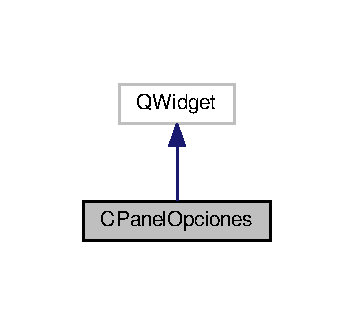
\includegraphics[width=170pt]{classCPanelOpciones__inherit__graph}
\end{center}
\end{figure}


Collaboration diagram for C\+Panel\+Opciones\+:
\nopagebreak
\begin{figure}[H]
\begin{center}
\leavevmode
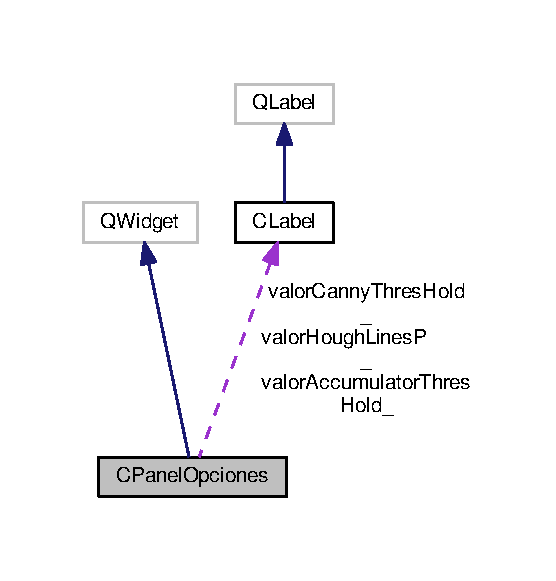
\includegraphics[width=267pt]{classCPanelOpciones__coll__graph}
\end{center}
\end{figure}
\subsection*{Public Member Functions}
\begin{DoxyCompactItemize}
\item 
\hyperlink{classCPanelOpciones_ad187a964b9ac72e6571ca699035195a3}{C\+Panel\+Opciones} ()
\begin{DoxyCompactList}\small\item\em Constructor de la clase. \end{DoxyCompactList}\item 
Q\+Scroll\+Bar $\ast$ \hyperlink{classCPanelOpciones_a69b8584e61b0fbd7a86c9b4b1af4fd60}{get\+Canny\+Thres\+Hold} ()
\begin{DoxyCompactList}\small\item\em Metodo que retorna el Q\+Scroll\+Bar de la Variable Canny\+Thres\+Hold. \end{DoxyCompactList}\item 
Q\+Scroll\+Bar $\ast$ \hyperlink{classCPanelOpciones_adefbced180846a9e7443aa6063ea39f8}{get\+Accumulator\+Thres\+Hold} ()
\begin{DoxyCompactList}\small\item\em Metodo que retorna el Q\+Scroll\+Bar de la Variable Accumulator\+Thres\+Hold. \end{DoxyCompactList}\item 
Q\+Scroll\+Bar $\ast$ \hyperlink{classCPanelOpciones_a26734902c1b8c353c83c6b3530be3c47}{get\+Hough\+LinesP} ()
\begin{DoxyCompactList}\small\item\em Metodo que retorna el Q\+Scroll\+Bar de la Variable hough\+LinesP. \end{DoxyCompactList}\item 
\hyperlink{classCLabel}{C\+Label} $\ast$ \hyperlink{classCPanelOpciones_a65fee0477e988937ea93176f04657388}{get\+Valor\+Canny\+Thres\+Hold} ()
\begin{DoxyCompactList}\small\item\em Metodo que retorna el \hyperlink{classCLabel}{C\+Label} de la Variable Canny\+Thres\+Hold. \end{DoxyCompactList}\item 
\hyperlink{classCLabel}{C\+Label} $\ast$ \hyperlink{classCPanelOpciones_a0f051efb1549353b79966471bc6b656f}{get\+Valor\+Accumulator\+Thres\+Hold} ()
\begin{DoxyCompactList}\small\item\em Metodo que retorna el \hyperlink{classCLabel}{C\+Label} de la Variable Accumulator\+Thres\+Hold. \end{DoxyCompactList}\item 
\hyperlink{classCLabel}{C\+Label} $\ast$ \hyperlink{classCPanelOpciones_aae4983463e8d5e2d07fc93bee488af0b}{get\+Valor\+Hough\+LinesP} ()
\begin{DoxyCompactList}\small\item\em Metodo que retorna el \hyperlink{classCLabel}{C\+Label} de la Variable Hough\+LinesP. \end{DoxyCompactList}\end{DoxyCompactItemize}
\subsection*{Private Attributes}
\begin{DoxyCompactItemize}
\item 
Q\+Scroll\+Bar $\ast$ \hyperlink{classCPanelOpciones_a02b5fec0793280de210c64541fc47155}{canny\+Thres\+Hold\+\_\+}
\begin{DoxyCompactList}\small\item\em Q\+Scroll\+Bar variable canny\+Thres\+Hold por defecto a 30. Utilizada en la deteccion de circulos. \end{DoxyCompactList}\item 
Q\+Scroll\+Bar $\ast$ \hyperlink{classCPanelOpciones_a1d0f21eb4ba18ebcfd6068817f17bef2}{accumulator\+Thres\+Hold\+\_\+}
\begin{DoxyCompactList}\small\item\em Q\+Scroll\+Bar variable accumulator\+Thres\+Hold por defecto a 42. Utilizada en la deteccion de circulos. \end{DoxyCompactList}\item 
Q\+Scroll\+Bar $\ast$ \hyperlink{classCPanelOpciones_a8e5bbb65d75f9dec3623b1796465c583}{houg\+Lines\+P\+\_\+}
\begin{DoxyCompactList}\small\item\em Q\+Scroll\+Bar variable hough\+LinesP por defecto 80. Utilizada en la deteccion de lineas. \end{DoxyCompactList}\item 
\hyperlink{classCLabel}{C\+Label} $\ast$ \hyperlink{classCPanelOpciones_a09a2c503f1520a71866669fd84b95ebf}{valor\+Canny\+Thres\+Hold\+\_\+}
\begin{DoxyCompactList}\small\item\em \hyperlink{classCLabel}{C\+Label} variable canny\+Thres\+Hold. \end{DoxyCompactList}\item 
\hyperlink{classCLabel}{C\+Label} $\ast$ \hyperlink{classCPanelOpciones_a206f20e0afadfa1bfda3c59cd2ca16b2}{valor\+Accumulator\+Thres\+Hold\+\_\+}
\begin{DoxyCompactList}\small\item\em \hyperlink{classCLabel}{C\+Label} variable accumulator\+Thres\+Hold. \end{DoxyCompactList}\item 
\hyperlink{classCLabel}{C\+Label} $\ast$ \hyperlink{classCPanelOpciones_ab415dcfa099eb5bc1fe6e576fe50e4ca}{valor\+Hough\+Lines\+P\+\_\+}
\begin{DoxyCompactList}\small\item\em \hyperlink{classCLabel}{C\+Label} variable hough\+LinesP. \end{DoxyCompactList}\end{DoxyCompactItemize}


\subsection{Detailed Description}
Clase que almacena un panel con las variables de la Detección de circulos y lineas. 

\subsection{Constructor \& Destructor Documentation}
\index{C\+Panel\+Opciones@{C\+Panel\+Opciones}!C\+Panel\+Opciones@{C\+Panel\+Opciones}}
\index{C\+Panel\+Opciones@{C\+Panel\+Opciones}!C\+Panel\+Opciones@{C\+Panel\+Opciones}}
\subsubsection[{\texorpdfstring{C\+Panel\+Opciones()}{CPanelOpciones()}}]{\setlength{\rightskip}{0pt plus 5cm}C\+Panel\+Opciones\+::\+C\+Panel\+Opciones (
\begin{DoxyParamCaption}
{}
\end{DoxyParamCaption}
)}\hypertarget{classCPanelOpciones_ad187a964b9ac72e6571ca699035195a3}{}\label{classCPanelOpciones_ad187a964b9ac72e6571ca699035195a3}


Constructor de la clase. 

Se carga el Layout del panel

Se inicializan los Q\+Scroll\+Bar

Aplicamos estilo fondo \textquotesingle{}verde\textquotesingle{}, rango de valores y valor por defecto a los Q\+Scroll\+Bar

Se inicializan los \hyperlink{classCLabel}{C\+Label} con los valores de los Q\+Scroll\+Bar

Agregamos a la ventana los datos 

\subsection{Member Function Documentation}
\index{C\+Panel\+Opciones@{C\+Panel\+Opciones}!get\+Accumulator\+Thres\+Hold@{get\+Accumulator\+Thres\+Hold}}
\index{get\+Accumulator\+Thres\+Hold@{get\+Accumulator\+Thres\+Hold}!C\+Panel\+Opciones@{C\+Panel\+Opciones}}
\subsubsection[{\texorpdfstring{get\+Accumulator\+Thres\+Hold()}{getAccumulatorThresHold()}}]{\setlength{\rightskip}{0pt plus 5cm}Q\+Scroll\+Bar $\ast$ C\+Panel\+Opciones\+::get\+Accumulator\+Thres\+Hold (
\begin{DoxyParamCaption}
{}
\end{DoxyParamCaption}
)}\hypertarget{classCPanelOpciones_adefbced180846a9e7443aa6063ea39f8}{}\label{classCPanelOpciones_adefbced180846a9e7443aa6063ea39f8}


Metodo que retorna el Q\+Scroll\+Bar de la Variable Accumulator\+Thres\+Hold. 

\begin{DoxyReturn}{Returns}
Q\+Scroll\+Bar 
\end{DoxyReturn}
\index{C\+Panel\+Opciones@{C\+Panel\+Opciones}!get\+Canny\+Thres\+Hold@{get\+Canny\+Thres\+Hold}}
\index{get\+Canny\+Thres\+Hold@{get\+Canny\+Thres\+Hold}!C\+Panel\+Opciones@{C\+Panel\+Opciones}}
\subsubsection[{\texorpdfstring{get\+Canny\+Thres\+Hold()}{getCannyThresHold()}}]{\setlength{\rightskip}{0pt plus 5cm}Q\+Scroll\+Bar $\ast$ C\+Panel\+Opciones\+::get\+Canny\+Thres\+Hold (
\begin{DoxyParamCaption}
{}
\end{DoxyParamCaption}
)}\hypertarget{classCPanelOpciones_a69b8584e61b0fbd7a86c9b4b1af4fd60}{}\label{classCPanelOpciones_a69b8584e61b0fbd7a86c9b4b1af4fd60}


Metodo que retorna el Q\+Scroll\+Bar de la Variable Canny\+Thres\+Hold. 

\begin{DoxyReturn}{Returns}
Q\+Scroll\+Bar 
\end{DoxyReturn}
\index{C\+Panel\+Opciones@{C\+Panel\+Opciones}!get\+Hough\+LinesP@{get\+Hough\+LinesP}}
\index{get\+Hough\+LinesP@{get\+Hough\+LinesP}!C\+Panel\+Opciones@{C\+Panel\+Opciones}}
\subsubsection[{\texorpdfstring{get\+Hough\+Lines\+P()}{getHoughLinesP()}}]{\setlength{\rightskip}{0pt plus 5cm}Q\+Scroll\+Bar $\ast$ C\+Panel\+Opciones\+::get\+Hough\+LinesP (
\begin{DoxyParamCaption}
{}
\end{DoxyParamCaption}
)}\hypertarget{classCPanelOpciones_a26734902c1b8c353c83c6b3530be3c47}{}\label{classCPanelOpciones_a26734902c1b8c353c83c6b3530be3c47}


Metodo que retorna el Q\+Scroll\+Bar de la Variable hough\+LinesP. 

\begin{DoxyReturn}{Returns}

\end{DoxyReturn}
\index{C\+Panel\+Opciones@{C\+Panel\+Opciones}!get\+Valor\+Accumulator\+Thres\+Hold@{get\+Valor\+Accumulator\+Thres\+Hold}}
\index{get\+Valor\+Accumulator\+Thres\+Hold@{get\+Valor\+Accumulator\+Thres\+Hold}!C\+Panel\+Opciones@{C\+Panel\+Opciones}}
\subsubsection[{\texorpdfstring{get\+Valor\+Accumulator\+Thres\+Hold()}{getValorAccumulatorThresHold()}}]{\setlength{\rightskip}{0pt plus 5cm}{\bf C\+Label} $\ast$ C\+Panel\+Opciones\+::get\+Valor\+Accumulator\+Thres\+Hold (
\begin{DoxyParamCaption}
{}
\end{DoxyParamCaption}
)}\hypertarget{classCPanelOpciones_a0f051efb1549353b79966471bc6b656f}{}\label{classCPanelOpciones_a0f051efb1549353b79966471bc6b656f}


Metodo que retorna el \hyperlink{classCLabel}{C\+Label} de la Variable Accumulator\+Thres\+Hold. 

\begin{DoxyReturn}{Returns}
\hyperlink{classCLabel}{C\+Label} 
\end{DoxyReturn}
\index{C\+Panel\+Opciones@{C\+Panel\+Opciones}!get\+Valor\+Canny\+Thres\+Hold@{get\+Valor\+Canny\+Thres\+Hold}}
\index{get\+Valor\+Canny\+Thres\+Hold@{get\+Valor\+Canny\+Thres\+Hold}!C\+Panel\+Opciones@{C\+Panel\+Opciones}}
\subsubsection[{\texorpdfstring{get\+Valor\+Canny\+Thres\+Hold()}{getValorCannyThresHold()}}]{\setlength{\rightskip}{0pt plus 5cm}{\bf C\+Label} $\ast$ C\+Panel\+Opciones\+::get\+Valor\+Canny\+Thres\+Hold (
\begin{DoxyParamCaption}
{}
\end{DoxyParamCaption}
)}\hypertarget{classCPanelOpciones_a65fee0477e988937ea93176f04657388}{}\label{classCPanelOpciones_a65fee0477e988937ea93176f04657388}


Metodo que retorna el \hyperlink{classCLabel}{C\+Label} de la Variable Canny\+Thres\+Hold. 

\begin{DoxyReturn}{Returns}
\hyperlink{classCLabel}{C\+Label} 
\end{DoxyReturn}
\index{C\+Panel\+Opciones@{C\+Panel\+Opciones}!get\+Valor\+Hough\+LinesP@{get\+Valor\+Hough\+LinesP}}
\index{get\+Valor\+Hough\+LinesP@{get\+Valor\+Hough\+LinesP}!C\+Panel\+Opciones@{C\+Panel\+Opciones}}
\subsubsection[{\texorpdfstring{get\+Valor\+Hough\+Lines\+P()}{getValorHoughLinesP()}}]{\setlength{\rightskip}{0pt plus 5cm}{\bf C\+Label} $\ast$ C\+Panel\+Opciones\+::get\+Valor\+Hough\+LinesP (
\begin{DoxyParamCaption}
{}
\end{DoxyParamCaption}
)}\hypertarget{classCPanelOpciones_aae4983463e8d5e2d07fc93bee488af0b}{}\label{classCPanelOpciones_aae4983463e8d5e2d07fc93bee488af0b}


Metodo que retorna el \hyperlink{classCLabel}{C\+Label} de la Variable Hough\+LinesP. 

\begin{DoxyReturn}{Returns}

\end{DoxyReturn}


\subsection{Member Data Documentation}
\index{C\+Panel\+Opciones@{C\+Panel\+Opciones}!accumulator\+Thres\+Hold\+\_\+@{accumulator\+Thres\+Hold\+\_\+}}
\index{accumulator\+Thres\+Hold\+\_\+@{accumulator\+Thres\+Hold\+\_\+}!C\+Panel\+Opciones@{C\+Panel\+Opciones}}
\subsubsection[{\texorpdfstring{accumulator\+Thres\+Hold\+\_\+}{accumulatorThresHold_}}]{\setlength{\rightskip}{0pt plus 5cm}Q\+Scroll\+Bar$\ast$ C\+Panel\+Opciones\+::accumulator\+Thres\+Hold\+\_\+\hspace{0.3cm}{\ttfamily [private]}}\hypertarget{classCPanelOpciones_a1d0f21eb4ba18ebcfd6068817f17bef2}{}\label{classCPanelOpciones_a1d0f21eb4ba18ebcfd6068817f17bef2}


Q\+Scroll\+Bar variable accumulator\+Thres\+Hold por defecto a 42. Utilizada en la deteccion de circulos. 

\index{C\+Panel\+Opciones@{C\+Panel\+Opciones}!canny\+Thres\+Hold\+\_\+@{canny\+Thres\+Hold\+\_\+}}
\index{canny\+Thres\+Hold\+\_\+@{canny\+Thres\+Hold\+\_\+}!C\+Panel\+Opciones@{C\+Panel\+Opciones}}
\subsubsection[{\texorpdfstring{canny\+Thres\+Hold\+\_\+}{cannyThresHold_}}]{\setlength{\rightskip}{0pt plus 5cm}Q\+Scroll\+Bar$\ast$ C\+Panel\+Opciones\+::canny\+Thres\+Hold\+\_\+\hspace{0.3cm}{\ttfamily [private]}}\hypertarget{classCPanelOpciones_a02b5fec0793280de210c64541fc47155}{}\label{classCPanelOpciones_a02b5fec0793280de210c64541fc47155}


Q\+Scroll\+Bar variable canny\+Thres\+Hold por defecto a 30. Utilizada en la deteccion de circulos. 

\index{C\+Panel\+Opciones@{C\+Panel\+Opciones}!houg\+Lines\+P\+\_\+@{houg\+Lines\+P\+\_\+}}
\index{houg\+Lines\+P\+\_\+@{houg\+Lines\+P\+\_\+}!C\+Panel\+Opciones@{C\+Panel\+Opciones}}
\subsubsection[{\texorpdfstring{houg\+Lines\+P\+\_\+}{hougLinesP_}}]{\setlength{\rightskip}{0pt plus 5cm}Q\+Scroll\+Bar$\ast$ C\+Panel\+Opciones\+::houg\+Lines\+P\+\_\+\hspace{0.3cm}{\ttfamily [private]}}\hypertarget{classCPanelOpciones_a8e5bbb65d75f9dec3623b1796465c583}{}\label{classCPanelOpciones_a8e5bbb65d75f9dec3623b1796465c583}


Q\+Scroll\+Bar variable hough\+LinesP por defecto 80. Utilizada en la deteccion de lineas. 

\index{C\+Panel\+Opciones@{C\+Panel\+Opciones}!valor\+Accumulator\+Thres\+Hold\+\_\+@{valor\+Accumulator\+Thres\+Hold\+\_\+}}
\index{valor\+Accumulator\+Thres\+Hold\+\_\+@{valor\+Accumulator\+Thres\+Hold\+\_\+}!C\+Panel\+Opciones@{C\+Panel\+Opciones}}
\subsubsection[{\texorpdfstring{valor\+Accumulator\+Thres\+Hold\+\_\+}{valorAccumulatorThresHold_}}]{\setlength{\rightskip}{0pt plus 5cm}{\bf C\+Label}$\ast$ C\+Panel\+Opciones\+::valor\+Accumulator\+Thres\+Hold\+\_\+\hspace{0.3cm}{\ttfamily [private]}}\hypertarget{classCPanelOpciones_a206f20e0afadfa1bfda3c59cd2ca16b2}{}\label{classCPanelOpciones_a206f20e0afadfa1bfda3c59cd2ca16b2}


\hyperlink{classCLabel}{C\+Label} variable accumulator\+Thres\+Hold. 

\index{C\+Panel\+Opciones@{C\+Panel\+Opciones}!valor\+Canny\+Thres\+Hold\+\_\+@{valor\+Canny\+Thres\+Hold\+\_\+}}
\index{valor\+Canny\+Thres\+Hold\+\_\+@{valor\+Canny\+Thres\+Hold\+\_\+}!C\+Panel\+Opciones@{C\+Panel\+Opciones}}
\subsubsection[{\texorpdfstring{valor\+Canny\+Thres\+Hold\+\_\+}{valorCannyThresHold_}}]{\setlength{\rightskip}{0pt plus 5cm}{\bf C\+Label}$\ast$ C\+Panel\+Opciones\+::valor\+Canny\+Thres\+Hold\+\_\+\hspace{0.3cm}{\ttfamily [private]}}\hypertarget{classCPanelOpciones_a09a2c503f1520a71866669fd84b95ebf}{}\label{classCPanelOpciones_a09a2c503f1520a71866669fd84b95ebf}


\hyperlink{classCLabel}{C\+Label} variable canny\+Thres\+Hold. 

\index{C\+Panel\+Opciones@{C\+Panel\+Opciones}!valor\+Hough\+Lines\+P\+\_\+@{valor\+Hough\+Lines\+P\+\_\+}}
\index{valor\+Hough\+Lines\+P\+\_\+@{valor\+Hough\+Lines\+P\+\_\+}!C\+Panel\+Opciones@{C\+Panel\+Opciones}}
\subsubsection[{\texorpdfstring{valor\+Hough\+Lines\+P\+\_\+}{valorHoughLinesP_}}]{\setlength{\rightskip}{0pt plus 5cm}{\bf C\+Label}$\ast$ C\+Panel\+Opciones\+::valor\+Hough\+Lines\+P\+\_\+\hspace{0.3cm}{\ttfamily [private]}}\hypertarget{classCPanelOpciones_ab415dcfa099eb5bc1fe6e576fe50e4ca}{}\label{classCPanelOpciones_ab415dcfa099eb5bc1fe6e576fe50e4ca}


\hyperlink{classCLabel}{C\+Label} variable hough\+LinesP. 



The documentation for this class was generated from the following files\+:\begin{DoxyCompactItemize}
\item 
\hyperlink{CPanelOpciones_8h}{C\+Panel\+Opciones.\+h}\item 
\hyperlink{CPanelOpciones_8cpp}{C\+Panel\+Opciones.\+cpp}\end{DoxyCompactItemize}

\hypertarget{classCPushButton}{}\section{C\+Push\+Button Class Reference}
\label{classCPushButton}\index{C\+Push\+Button@{C\+Push\+Button}}


Clase heredada de \textquotesingle{}Q\+Push\+Button\textquotesingle{} que aplica un estilo determinado a este tipo de container.  




{\ttfamily \#include $<$C\+Push\+Button.\+h$>$}



Inheritance diagram for C\+Push\+Button\+:\nopagebreak
\begin{figure}[H]
\begin{center}
\leavevmode
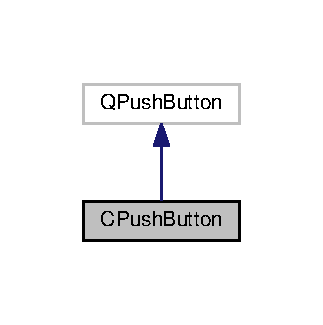
\includegraphics[width=155pt]{classCPushButton__inherit__graph}
\end{center}
\end{figure}


Collaboration diagram for C\+Push\+Button\+:\nopagebreak
\begin{figure}[H]
\begin{center}
\leavevmode
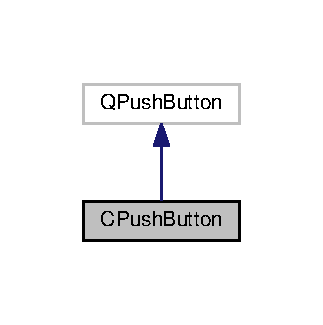
\includegraphics[width=155pt]{classCPushButton__coll__graph}
\end{center}
\end{figure}
\subsection*{Public Member Functions}
\begin{DoxyCompactItemize}
\item 
\hyperlink{classCPushButton_afbe6d5ef008dc7e41b14c4875ae0274b}{C\+Push\+Button} (Q\+String text, bool estilo)
\begin{DoxyCompactList}\small\item\em Constructor que aplica el estilo. \end{DoxyCompactList}\end{DoxyCompactItemize}


\subsection{Detailed Description}
Clase heredada de \textquotesingle{}Q\+Push\+Button\textquotesingle{} que aplica un estilo determinado a este tipo de container. 

\subsection{Constructor \& Destructor Documentation}
\index{C\+Push\+Button@{C\+Push\+Button}!C\+Push\+Button@{C\+Push\+Button}}
\index{C\+Push\+Button@{C\+Push\+Button}!C\+Push\+Button@{C\+Push\+Button}}
\subsubsection[{\texorpdfstring{C\+Push\+Button(\+Q\+String text, bool estilo)}{CPushButton(QString text, bool estilo)}}]{\setlength{\rightskip}{0pt plus 5cm}C\+Push\+Button\+::\+C\+Push\+Button (
\begin{DoxyParamCaption}
\item[{Q\+String}]{text, }
\item[{bool}]{estilo}
\end{DoxyParamCaption}
)}\hypertarget{classCPushButton_afbe6d5ef008dc7e41b14c4875ae0274b}{}\label{classCPushButton_afbe6d5ef008dc7e41b14c4875ae0274b}


Constructor que aplica el estilo. 


\begin{DoxyParams}{Parameters}
{\em text.} & Texto del Button \\
\hline
{\em estilo.} & Estilo utilizado, cambia el tamano de la letra \\
\hline
\end{DoxyParams}


The documentation for this class was generated from the following files\+:\begin{DoxyCompactItemize}
\item 
\hyperlink{CPushButton_8h}{C\+Push\+Button.\+h}\item 
\hyperlink{CPushButton_8cpp}{C\+Push\+Button.\+cpp}\end{DoxyCompactItemize}

\hypertarget{classCTransicion}{}\section{C\+Transicion Class Reference}
\label{classCTransicion}\index{C\+Transicion@{C\+Transicion}}


{\ttfamily \#include $<$C\+Transicion.\+h$>$}

\subsection*{Public Member Functions}
\begin{DoxyCompactItemize}
\item 
void \hyperlink{classCTransicion_a3bd402b9a500069fa3d7a8c6a622e859}{set\+Transicion} (int \hyperlink{classCTransicion_a6add557ec0b0aaaa974346f4f9dd1585}{q}, char \hyperlink{classCTransicion_a25058569b7c254796fa648be9bfe2222}{c}, int \hyperlink{classCTransicion_a9b95c9349367059e02de2e997ec3b2bb}{next\+\_\+q})
\item 
int \hyperlink{classCTransicion_aa1e8c8f2d8c1f9d5ffd3cd34480a0d4a}{get\+Estado\+\_\+origen} ()
\item 
int \hyperlink{classCTransicion_ab54e183e404c57679ef661bae3d8ce57}{get\+Estado\+\_\+siguiente} ()
\item 
char \hyperlink{classCTransicion_a37623a49e327367d5bab7d01c6dd7827}{get\+Caracter} ()
\item 
void \hyperlink{classCTransicion_acfeb5ccd4314048acd29fd1804f66d22}{Mostrar\+Transicion} ()
\end{DoxyCompactItemize}
\subsection*{Private Attributes}
\begin{DoxyCompactItemize}
\item 
int \hyperlink{classCTransicion_a6add557ec0b0aaaa974346f4f9dd1585}{q}
\item 
char \hyperlink{classCTransicion_a25058569b7c254796fa648be9bfe2222}{c}
\item 
int \hyperlink{classCTransicion_a9b95c9349367059e02de2e997ec3b2bb}{next\+\_\+q}
\end{DoxyCompactItemize}


\subsection{Member Function Documentation}
\index{C\+Transicion@{C\+Transicion}!get\+Caracter@{get\+Caracter}}
\index{get\+Caracter@{get\+Caracter}!C\+Transicion@{C\+Transicion}}
\subsubsection[{\texorpdfstring{get\+Caracter()}{getCaracter()}}]{\setlength{\rightskip}{0pt plus 5cm}char C\+Transicion\+::get\+Caracter (
\begin{DoxyParamCaption}
{}
\end{DoxyParamCaption}
)}\hypertarget{classCTransicion_a37623a49e327367d5bab7d01c6dd7827}{}\label{classCTransicion_a37623a49e327367d5bab7d01c6dd7827}
\index{C\+Transicion@{C\+Transicion}!get\+Estado\+\_\+origen@{get\+Estado\+\_\+origen}}
\index{get\+Estado\+\_\+origen@{get\+Estado\+\_\+origen}!C\+Transicion@{C\+Transicion}}
\subsubsection[{\texorpdfstring{get\+Estado\+\_\+origen()}{getEstado_origen()}}]{\setlength{\rightskip}{0pt plus 5cm}int C\+Transicion\+::get\+Estado\+\_\+origen (
\begin{DoxyParamCaption}
{}
\end{DoxyParamCaption}
)}\hypertarget{classCTransicion_aa1e8c8f2d8c1f9d5ffd3cd34480a0d4a}{}\label{classCTransicion_aa1e8c8f2d8c1f9d5ffd3cd34480a0d4a}
\index{C\+Transicion@{C\+Transicion}!get\+Estado\+\_\+siguiente@{get\+Estado\+\_\+siguiente}}
\index{get\+Estado\+\_\+siguiente@{get\+Estado\+\_\+siguiente}!C\+Transicion@{C\+Transicion}}
\subsubsection[{\texorpdfstring{get\+Estado\+\_\+siguiente()}{getEstado_siguiente()}}]{\setlength{\rightskip}{0pt plus 5cm}int C\+Transicion\+::get\+Estado\+\_\+siguiente (
\begin{DoxyParamCaption}
{}
\end{DoxyParamCaption}
)}\hypertarget{classCTransicion_ab54e183e404c57679ef661bae3d8ce57}{}\label{classCTransicion_ab54e183e404c57679ef661bae3d8ce57}
\index{C\+Transicion@{C\+Transicion}!Mostrar\+Transicion@{Mostrar\+Transicion}}
\index{Mostrar\+Transicion@{Mostrar\+Transicion}!C\+Transicion@{C\+Transicion}}
\subsubsection[{\texorpdfstring{Mostrar\+Transicion()}{MostrarTransicion()}}]{\setlength{\rightskip}{0pt plus 5cm}void C\+Transicion\+::\+Mostrar\+Transicion (
\begin{DoxyParamCaption}
{}
\end{DoxyParamCaption}
)}\hypertarget{classCTransicion_acfeb5ccd4314048acd29fd1804f66d22}{}\label{classCTransicion_acfeb5ccd4314048acd29fd1804f66d22}
\index{C\+Transicion@{C\+Transicion}!set\+Transicion@{set\+Transicion}}
\index{set\+Transicion@{set\+Transicion}!C\+Transicion@{C\+Transicion}}
\subsubsection[{\texorpdfstring{set\+Transicion(int q, char c, int next\+\_\+q)}{setTransicion(int q, char c, int next_q)}}]{\setlength{\rightskip}{0pt plus 5cm}void C\+Transicion\+::set\+Transicion (
\begin{DoxyParamCaption}
\item[{int}]{q, }
\item[{char}]{c, }
\item[{int}]{next\+\_\+q}
\end{DoxyParamCaption}
)}\hypertarget{classCTransicion_a3bd402b9a500069fa3d7a8c6a622e859}{}\label{classCTransicion_a3bd402b9a500069fa3d7a8c6a622e859}


\subsection{Member Data Documentation}
\index{C\+Transicion@{C\+Transicion}!c@{c}}
\index{c@{c}!C\+Transicion@{C\+Transicion}}
\subsubsection[{\texorpdfstring{c}{c}}]{\setlength{\rightskip}{0pt plus 5cm}char C\+Transicion\+::c\hspace{0.3cm}{\ttfamily [private]}}\hypertarget{classCTransicion_a25058569b7c254796fa648be9bfe2222}{}\label{classCTransicion_a25058569b7c254796fa648be9bfe2222}
\index{C\+Transicion@{C\+Transicion}!next\+\_\+q@{next\+\_\+q}}
\index{next\+\_\+q@{next\+\_\+q}!C\+Transicion@{C\+Transicion}}
\subsubsection[{\texorpdfstring{next\+\_\+q}{next_q}}]{\setlength{\rightskip}{0pt plus 5cm}int C\+Transicion\+::next\+\_\+q\hspace{0.3cm}{\ttfamily [private]}}\hypertarget{classCTransicion_a9b95c9349367059e02de2e997ec3b2bb}{}\label{classCTransicion_a9b95c9349367059e02de2e997ec3b2bb}
\index{C\+Transicion@{C\+Transicion}!q@{q}}
\index{q@{q}!C\+Transicion@{C\+Transicion}}
\subsubsection[{\texorpdfstring{q}{q}}]{\setlength{\rightskip}{0pt plus 5cm}int C\+Transicion\+::q\hspace{0.3cm}{\ttfamily [private]}}\hypertarget{classCTransicion_a6add557ec0b0aaaa974346f4f9dd1585}{}\label{classCTransicion_a6add557ec0b0aaaa974346f4f9dd1585}


The documentation for this class was generated from the following files\+:\begin{DoxyCompactItemize}
\item 
\hyperlink{CTransicion_8h}{C\+Transicion.\+h}\item 
\hyperlink{CTransicion_8cpp}{C\+Transicion.\+cpp}\end{DoxyCompactItemize}

\hypertarget{classDFA__MIN}{}\section{D\+F\+A\+\_\+\+M\+IN Class Reference}
\label{classDFA__MIN}\index{D\+F\+A\+\_\+\+M\+IN@{D\+F\+A\+\_\+\+M\+IN}}


{\ttfamily \#include $<$D\+F\+A\+\_\+min.\+h$>$}



Collaboration diagram for D\+F\+A\+\_\+\+M\+IN\+:
\nopagebreak
\begin{figure}[H]
\begin{center}
\leavevmode
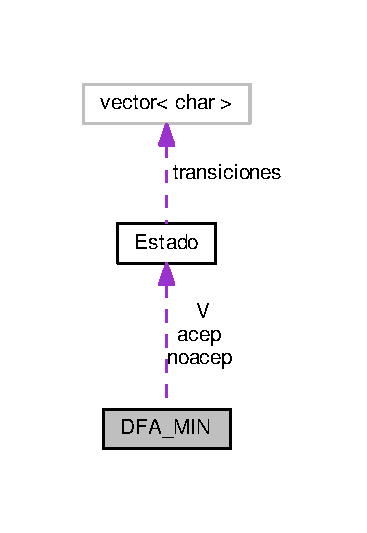
\includegraphics[width=176pt]{classDFA__MIN__coll__graph}
\end{center}
\end{figure}
\subsection*{Public Member Functions}
\begin{DoxyCompactItemize}
\item 
\hyperlink{classDFA__MIN_ab23d007d4a597b9242ec63b175c0d442}{D\+F\+A\+\_\+\+M\+IN} ()
\item 
\hyperlink{classDFA__MIN_abd44cdc58f7ac815124722ab26070c59}{$\sim$\+D\+F\+A\+\_\+\+M\+IN} ()
\item 
void \hyperlink{classDFA__MIN_a933ed65f474a79dd69bd77af2c9ab4fc}{Leer\+\_\+\+D\+FA} (char nombre\mbox{[}$\,$\mbox{]})
\item 
void \hyperlink{classDFA__MIN_a45f3039094bbb7dcd19de0c49419243f}{Exportar\+\_\+\+D\+F\+A\+\_\+min} ()
\item 
int \hyperlink{classDFA__MIN_af199da3ede7ed11204a754c2183aab08}{long\+\_\+cadena} (char $\ast$)
\item 
void \hyperlink{classDFA__MIN_a359c0fec7be50994213ab598c62c69ec}{Minimizar\+\_\+\+D\+FA} ()
\item 
void \hyperlink{classDFA__MIN_a02572f57610c3eaace394c5e487ab524}{Divide\+\_\+\+D\+FA} ()
\item 
int \hyperlink{classDFA__MIN_a63aceba3b4ca0527cde22afdb09c05a4}{Contador\+\_\+\+ID} (int id)
\item 
bool \hyperlink{classDFA__MIN_a23fffd70992a82b8f2f574dd2ddde71e}{Comprobar\+\_\+\+Trans} (int id\+\_\+conj, char id\+\_\+trans, int n\+\_\+trans)
\item 
char \hyperlink{classDFA__MIN_a7d8b26d37ceb44ee9f2da46b849096a1}{Buscar\+Estado} (char est)
\item 
void \hyperlink{classDFA__MIN_aa739fb89570a82ff0af1997e2cf05e8d}{Cambia\+\_\+\+Estado} (char id, char rep)
\item 
void \hyperlink{classDFA__MIN_a3c7227b8f88987417625b25ec0410fe8}{Cambia\+\_\+\+Conjunto} (\hyperlink{classEstado}{Estado} $\ast$vec, int tam, char id, char tra, char conj)
\item 
void \hyperlink{classDFA__MIN_a0facf3c8cea99d1235593bf2b65e0e4e}{Transforma\+\_\+\+Conj} (\hyperlink{classEstado}{Estado} $\ast$vec, int tam)
\item 
void \hyperlink{classDFA__MIN_a9d98e8fe7dbd789624ed083484a5c04a}{Min\+\_\+\+V\+Ec} (\hyperlink{classEstado}{Estado} $\ast$vec, int tam, int x)
\item 
int \hyperlink{classDFA__MIN_ad025e5ebeb4dcca68a1e27d0f91d0b27}{Oculta\+\_\+\+Estados} (\hyperlink{classEstado}{Estado} $\ast$vec, int tam, int res)
\item 
void \hyperlink{classDFA__MIN_acbb53157090bbfa6fee78eadab964082}{Check\+\_\+\+Trans} ()
\item 
void \hyperlink{classDFA__MIN_af3f05b252ab137139773054ba0596130}{Borrar\+\_\+\+Estados} ()
\end{DoxyCompactItemize}
\subsection*{Private Attributes}
\begin{DoxyCompactItemize}
\item 
\hyperlink{classEstado}{Estado} $\ast$ \hyperlink{classDFA__MIN_a63e88c71f42528401f723e7b0a1546b7}{V}
\item 
int \hyperlink{classDFA__MIN_afdb3a42ec5ff49939f83da7d524ecad4}{num\+\_\+est}
\item 
int \hyperlink{classDFA__MIN_a6c736ede2fcc8d8e367cdcfdb4dc16ab}{est\+\_\+ini}
\item 
int \hyperlink{classDFA__MIN_a2fae453e70c67af71d1cd70a16373d82}{cont\+\_\+id\+\_\+conj}
\item 
\hyperlink{classEstado}{Estado} $\ast$ \hyperlink{classDFA__MIN_a7105979d0dfe2f5aebe6a74286e93eda}{acep}
\item 
\hyperlink{classEstado}{Estado} $\ast$ \hyperlink{classDFA__MIN_aa3f8b663143a7c3a176ac7d0954ae82f}{noacep}
\item 
int \hyperlink{classDFA__MIN_a5e91293deaa7c83832e55f5177e31232}{cont\+\_\+acep}
\end{DoxyCompactItemize}


\subsection{Constructor \& Destructor Documentation}
\index{D\+F\+A\+\_\+\+M\+IN@{D\+F\+A\+\_\+\+M\+IN}!D\+F\+A\+\_\+\+M\+IN@{D\+F\+A\+\_\+\+M\+IN}}
\index{D\+F\+A\+\_\+\+M\+IN@{D\+F\+A\+\_\+\+M\+IN}!D\+F\+A\+\_\+\+M\+IN@{D\+F\+A\+\_\+\+M\+IN}}
\subsubsection[{\texorpdfstring{D\+F\+A\+\_\+\+M\+I\+N()}{DFA_MIN()}}]{\setlength{\rightskip}{0pt plus 5cm}D\+F\+A\+\_\+\+M\+I\+N\+::\+D\+F\+A\+\_\+\+M\+IN (
\begin{DoxyParamCaption}
{}
\end{DoxyParamCaption}
)}\hypertarget{classDFA__MIN_ab23d007d4a597b9242ec63b175c0d442}{}\label{classDFA__MIN_ab23d007d4a597b9242ec63b175c0d442}
\index{D\+F\+A\+\_\+\+M\+IN@{D\+F\+A\+\_\+\+M\+IN}!````~D\+F\+A\+\_\+\+M\+IN@{$\sim$\+D\+F\+A\+\_\+\+M\+IN}}
\index{````~D\+F\+A\+\_\+\+M\+IN@{$\sim$\+D\+F\+A\+\_\+\+M\+IN}!D\+F\+A\+\_\+\+M\+IN@{D\+F\+A\+\_\+\+M\+IN}}
\subsubsection[{\texorpdfstring{$\sim$\+D\+F\+A\+\_\+\+M\+I\+N()}{~DFA_MIN()}}]{\setlength{\rightskip}{0pt plus 5cm}D\+F\+A\+\_\+\+M\+I\+N\+::$\sim$\+D\+F\+A\+\_\+\+M\+IN (
\begin{DoxyParamCaption}
{}
\end{DoxyParamCaption}
)}\hypertarget{classDFA__MIN_abd44cdc58f7ac815124722ab26070c59}{}\label{classDFA__MIN_abd44cdc58f7ac815124722ab26070c59}


\subsection{Member Function Documentation}
\index{D\+F\+A\+\_\+\+M\+IN@{D\+F\+A\+\_\+\+M\+IN}!Borrar\+\_\+\+Estados@{Borrar\+\_\+\+Estados}}
\index{Borrar\+\_\+\+Estados@{Borrar\+\_\+\+Estados}!D\+F\+A\+\_\+\+M\+IN@{D\+F\+A\+\_\+\+M\+IN}}
\subsubsection[{\texorpdfstring{Borrar\+\_\+\+Estados()}{Borrar_Estados()}}]{\setlength{\rightskip}{0pt plus 5cm}void D\+F\+A\+\_\+\+M\+I\+N\+::\+Borrar\+\_\+\+Estados (
\begin{DoxyParamCaption}
{}
\end{DoxyParamCaption}
)}\hypertarget{classDFA__MIN_af3f05b252ab137139773054ba0596130}{}\label{classDFA__MIN_af3f05b252ab137139773054ba0596130}
\index{D\+F\+A\+\_\+\+M\+IN@{D\+F\+A\+\_\+\+M\+IN}!Buscar\+Estado@{Buscar\+Estado}}
\index{Buscar\+Estado@{Buscar\+Estado}!D\+F\+A\+\_\+\+M\+IN@{D\+F\+A\+\_\+\+M\+IN}}
\subsubsection[{\texorpdfstring{Buscar\+Estado(char est)}{BuscarEstado(char est)}}]{\setlength{\rightskip}{0pt plus 5cm}char D\+F\+A\+\_\+\+M\+I\+N\+::\+Buscar\+Estado (
\begin{DoxyParamCaption}
\item[{char}]{est}
\end{DoxyParamCaption}
)}\hypertarget{classDFA__MIN_a7d8b26d37ceb44ee9f2da46b849096a1}{}\label{classDFA__MIN_a7d8b26d37ceb44ee9f2da46b849096a1}
\index{D\+F\+A\+\_\+\+M\+IN@{D\+F\+A\+\_\+\+M\+IN}!Cambia\+\_\+\+Conjunto@{Cambia\+\_\+\+Conjunto}}
\index{Cambia\+\_\+\+Conjunto@{Cambia\+\_\+\+Conjunto}!D\+F\+A\+\_\+\+M\+IN@{D\+F\+A\+\_\+\+M\+IN}}
\subsubsection[{\texorpdfstring{Cambia\+\_\+\+Conjunto(\+Estado $\ast$vec, int tam, char id, char tra, char conj)}{Cambia_Conjunto(Estado *vec, int tam, char id, char tra, char conj)}}]{\setlength{\rightskip}{0pt plus 5cm}void D\+F\+A\+\_\+\+M\+I\+N\+::\+Cambia\+\_\+\+Conjunto (
\begin{DoxyParamCaption}
\item[{{\bf Estado} $\ast$}]{vec, }
\item[{int}]{tam, }
\item[{char}]{id, }
\item[{char}]{tra, }
\item[{char}]{conj}
\end{DoxyParamCaption}
)}\hypertarget{classDFA__MIN_a3c7227b8f88987417625b25ec0410fe8}{}\label{classDFA__MIN_a3c7227b8f88987417625b25ec0410fe8}
\index{D\+F\+A\+\_\+\+M\+IN@{D\+F\+A\+\_\+\+M\+IN}!Cambia\+\_\+\+Estado@{Cambia\+\_\+\+Estado}}
\index{Cambia\+\_\+\+Estado@{Cambia\+\_\+\+Estado}!D\+F\+A\+\_\+\+M\+IN@{D\+F\+A\+\_\+\+M\+IN}}
\subsubsection[{\texorpdfstring{Cambia\+\_\+\+Estado(char id, char rep)}{Cambia_Estado(char id, char rep)}}]{\setlength{\rightskip}{0pt plus 5cm}void D\+F\+A\+\_\+\+M\+I\+N\+::\+Cambia\+\_\+\+Estado (
\begin{DoxyParamCaption}
\item[{char}]{id, }
\item[{char}]{rep}
\end{DoxyParamCaption}
)}\hypertarget{classDFA__MIN_aa739fb89570a82ff0af1997e2cf05e8d}{}\label{classDFA__MIN_aa739fb89570a82ff0af1997e2cf05e8d}
\index{D\+F\+A\+\_\+\+M\+IN@{D\+F\+A\+\_\+\+M\+IN}!Check\+\_\+\+Trans@{Check\+\_\+\+Trans}}
\index{Check\+\_\+\+Trans@{Check\+\_\+\+Trans}!D\+F\+A\+\_\+\+M\+IN@{D\+F\+A\+\_\+\+M\+IN}}
\subsubsection[{\texorpdfstring{Check\+\_\+\+Trans()}{Check_Trans()}}]{\setlength{\rightskip}{0pt plus 5cm}void D\+F\+A\+\_\+\+M\+I\+N\+::\+Check\+\_\+\+Trans (
\begin{DoxyParamCaption}
{}
\end{DoxyParamCaption}
)}\hypertarget{classDFA__MIN_acbb53157090bbfa6fee78eadab964082}{}\label{classDFA__MIN_acbb53157090bbfa6fee78eadab964082}
\index{D\+F\+A\+\_\+\+M\+IN@{D\+F\+A\+\_\+\+M\+IN}!Comprobar\+\_\+\+Trans@{Comprobar\+\_\+\+Trans}}
\index{Comprobar\+\_\+\+Trans@{Comprobar\+\_\+\+Trans}!D\+F\+A\+\_\+\+M\+IN@{D\+F\+A\+\_\+\+M\+IN}}
\subsubsection[{\texorpdfstring{Comprobar\+\_\+\+Trans(int id\+\_\+conj, char id\+\_\+trans, int n\+\_\+trans)}{Comprobar_Trans(int id_conj, char id_trans, int n_trans)}}]{\setlength{\rightskip}{0pt plus 5cm}bool D\+F\+A\+\_\+\+M\+I\+N\+::\+Comprobar\+\_\+\+Trans (
\begin{DoxyParamCaption}
\item[{int}]{id\+\_\+conj, }
\item[{char}]{id\+\_\+trans, }
\item[{int}]{n\+\_\+trans}
\end{DoxyParamCaption}
)}\hypertarget{classDFA__MIN_a23fffd70992a82b8f2f574dd2ddde71e}{}\label{classDFA__MIN_a23fffd70992a82b8f2f574dd2ddde71e}
\index{D\+F\+A\+\_\+\+M\+IN@{D\+F\+A\+\_\+\+M\+IN}!Contador\+\_\+\+ID@{Contador\+\_\+\+ID}}
\index{Contador\+\_\+\+ID@{Contador\+\_\+\+ID}!D\+F\+A\+\_\+\+M\+IN@{D\+F\+A\+\_\+\+M\+IN}}
\subsubsection[{\texorpdfstring{Contador\+\_\+\+I\+D(int id)}{Contador_ID(int id)}}]{\setlength{\rightskip}{0pt plus 5cm}int D\+F\+A\+\_\+\+M\+I\+N\+::\+Contador\+\_\+\+ID (
\begin{DoxyParamCaption}
\item[{int}]{id}
\end{DoxyParamCaption}
)}\hypertarget{classDFA__MIN_a63aceba3b4ca0527cde22afdb09c05a4}{}\label{classDFA__MIN_a63aceba3b4ca0527cde22afdb09c05a4}
\index{D\+F\+A\+\_\+\+M\+IN@{D\+F\+A\+\_\+\+M\+IN}!Divide\+\_\+\+D\+FA@{Divide\+\_\+\+D\+FA}}
\index{Divide\+\_\+\+D\+FA@{Divide\+\_\+\+D\+FA}!D\+F\+A\+\_\+\+M\+IN@{D\+F\+A\+\_\+\+M\+IN}}
\subsubsection[{\texorpdfstring{Divide\+\_\+\+D\+F\+A()}{Divide_DFA()}}]{\setlength{\rightskip}{0pt plus 5cm}void D\+F\+A\+\_\+\+M\+I\+N\+::\+Divide\+\_\+\+D\+FA (
\begin{DoxyParamCaption}
{}
\end{DoxyParamCaption}
)}\hypertarget{classDFA__MIN_a02572f57610c3eaace394c5e487ab524}{}\label{classDFA__MIN_a02572f57610c3eaace394c5e487ab524}
\index{D\+F\+A\+\_\+\+M\+IN@{D\+F\+A\+\_\+\+M\+IN}!Exportar\+\_\+\+D\+F\+A\+\_\+min@{Exportar\+\_\+\+D\+F\+A\+\_\+min}}
\index{Exportar\+\_\+\+D\+F\+A\+\_\+min@{Exportar\+\_\+\+D\+F\+A\+\_\+min}!D\+F\+A\+\_\+\+M\+IN@{D\+F\+A\+\_\+\+M\+IN}}
\subsubsection[{\texorpdfstring{Exportar\+\_\+\+D\+F\+A\+\_\+min()}{Exportar_DFA_min()}}]{\setlength{\rightskip}{0pt plus 5cm}void D\+F\+A\+\_\+\+M\+I\+N\+::\+Exportar\+\_\+\+D\+F\+A\+\_\+min (
\begin{DoxyParamCaption}
{}
\end{DoxyParamCaption}
)}\hypertarget{classDFA__MIN_a45f3039094bbb7dcd19de0c49419243f}{}\label{classDFA__MIN_a45f3039094bbb7dcd19de0c49419243f}
\index{D\+F\+A\+\_\+\+M\+IN@{D\+F\+A\+\_\+\+M\+IN}!Leer\+\_\+\+D\+FA@{Leer\+\_\+\+D\+FA}}
\index{Leer\+\_\+\+D\+FA@{Leer\+\_\+\+D\+FA}!D\+F\+A\+\_\+\+M\+IN@{D\+F\+A\+\_\+\+M\+IN}}
\subsubsection[{\texorpdfstring{Leer\+\_\+\+D\+F\+A(char nombre[])}{Leer_DFA(char nombre[])}}]{\setlength{\rightskip}{0pt plus 5cm}void D\+F\+A\+\_\+\+M\+I\+N\+::\+Leer\+\_\+\+D\+FA (
\begin{DoxyParamCaption}
\item[{char}]{nombre\mbox{[}$\,$\mbox{]}}
\end{DoxyParamCaption}
)}\hypertarget{classDFA__MIN_a933ed65f474a79dd69bd77af2c9ab4fc}{}\label{classDFA__MIN_a933ed65f474a79dd69bd77af2c9ab4fc}
\index{D\+F\+A\+\_\+\+M\+IN@{D\+F\+A\+\_\+\+M\+IN}!long\+\_\+cadena@{long\+\_\+cadena}}
\index{long\+\_\+cadena@{long\+\_\+cadena}!D\+F\+A\+\_\+\+M\+IN@{D\+F\+A\+\_\+\+M\+IN}}
\subsubsection[{\texorpdfstring{long\+\_\+cadena(char $\ast$)}{long_cadena(char *)}}]{\setlength{\rightskip}{0pt plus 5cm}int D\+F\+A\+\_\+\+M\+I\+N\+::long\+\_\+cadena (
\begin{DoxyParamCaption}
\item[{char $\ast$}]{cadena}
\end{DoxyParamCaption}
)}\hypertarget{classDFA__MIN_af199da3ede7ed11204a754c2183aab08}{}\label{classDFA__MIN_af199da3ede7ed11204a754c2183aab08}
\index{D\+F\+A\+\_\+\+M\+IN@{D\+F\+A\+\_\+\+M\+IN}!Min\+\_\+\+V\+Ec@{Min\+\_\+\+V\+Ec}}
\index{Min\+\_\+\+V\+Ec@{Min\+\_\+\+V\+Ec}!D\+F\+A\+\_\+\+M\+IN@{D\+F\+A\+\_\+\+M\+IN}}
\subsubsection[{\texorpdfstring{Min\+\_\+\+V\+Ec(\+Estado $\ast$vec, int tam, int x)}{Min_VEc(Estado *vec, int tam, int x)}}]{\setlength{\rightskip}{0pt plus 5cm}void D\+F\+A\+\_\+\+M\+I\+N\+::\+Min\+\_\+\+V\+Ec (
\begin{DoxyParamCaption}
\item[{{\bf Estado} $\ast$}]{vec, }
\item[{int}]{tam, }
\item[{int}]{x}
\end{DoxyParamCaption}
)}\hypertarget{classDFA__MIN_a9d98e8fe7dbd789624ed083484a5c04a}{}\label{classDFA__MIN_a9d98e8fe7dbd789624ed083484a5c04a}
\index{D\+F\+A\+\_\+\+M\+IN@{D\+F\+A\+\_\+\+M\+IN}!Minimizar\+\_\+\+D\+FA@{Minimizar\+\_\+\+D\+FA}}
\index{Minimizar\+\_\+\+D\+FA@{Minimizar\+\_\+\+D\+FA}!D\+F\+A\+\_\+\+M\+IN@{D\+F\+A\+\_\+\+M\+IN}}
\subsubsection[{\texorpdfstring{Minimizar\+\_\+\+D\+F\+A()}{Minimizar_DFA()}}]{\setlength{\rightskip}{0pt plus 5cm}void D\+F\+A\+\_\+\+M\+I\+N\+::\+Minimizar\+\_\+\+D\+FA (
\begin{DoxyParamCaption}
{}
\end{DoxyParamCaption}
)}\hypertarget{classDFA__MIN_a359c0fec7be50994213ab598c62c69ec}{}\label{classDFA__MIN_a359c0fec7be50994213ab598c62c69ec}
\index{D\+F\+A\+\_\+\+M\+IN@{D\+F\+A\+\_\+\+M\+IN}!Oculta\+\_\+\+Estados@{Oculta\+\_\+\+Estados}}
\index{Oculta\+\_\+\+Estados@{Oculta\+\_\+\+Estados}!D\+F\+A\+\_\+\+M\+IN@{D\+F\+A\+\_\+\+M\+IN}}
\subsubsection[{\texorpdfstring{Oculta\+\_\+\+Estados(\+Estado $\ast$vec, int tam, int res)}{Oculta_Estados(Estado *vec, int tam, int res)}}]{\setlength{\rightskip}{0pt plus 5cm}int D\+F\+A\+\_\+\+M\+I\+N\+::\+Oculta\+\_\+\+Estados (
\begin{DoxyParamCaption}
\item[{{\bf Estado} $\ast$}]{vec, }
\item[{int}]{tam, }
\item[{int}]{res}
\end{DoxyParamCaption}
)}\hypertarget{classDFA__MIN_ad025e5ebeb4dcca68a1e27d0f91d0b27}{}\label{classDFA__MIN_ad025e5ebeb4dcca68a1e27d0f91d0b27}
\index{D\+F\+A\+\_\+\+M\+IN@{D\+F\+A\+\_\+\+M\+IN}!Transforma\+\_\+\+Conj@{Transforma\+\_\+\+Conj}}
\index{Transforma\+\_\+\+Conj@{Transforma\+\_\+\+Conj}!D\+F\+A\+\_\+\+M\+IN@{D\+F\+A\+\_\+\+M\+IN}}
\subsubsection[{\texorpdfstring{Transforma\+\_\+\+Conj(\+Estado $\ast$vec, int tam)}{Transforma_Conj(Estado *vec, int tam)}}]{\setlength{\rightskip}{0pt plus 5cm}void D\+F\+A\+\_\+\+M\+I\+N\+::\+Transforma\+\_\+\+Conj (
\begin{DoxyParamCaption}
\item[{{\bf Estado} $\ast$}]{vec, }
\item[{int}]{tam}
\end{DoxyParamCaption}
)}\hypertarget{classDFA__MIN_a0facf3c8cea99d1235593bf2b65e0e4e}{}\label{classDFA__MIN_a0facf3c8cea99d1235593bf2b65e0e4e}


\subsection{Member Data Documentation}
\index{D\+F\+A\+\_\+\+M\+IN@{D\+F\+A\+\_\+\+M\+IN}!acep@{acep}}
\index{acep@{acep}!D\+F\+A\+\_\+\+M\+IN@{D\+F\+A\+\_\+\+M\+IN}}
\subsubsection[{\texorpdfstring{acep}{acep}}]{\setlength{\rightskip}{0pt plus 5cm}{\bf Estado}$\ast$ D\+F\+A\+\_\+\+M\+I\+N\+::acep\hspace{0.3cm}{\ttfamily [private]}}\hypertarget{classDFA__MIN_a7105979d0dfe2f5aebe6a74286e93eda}{}\label{classDFA__MIN_a7105979d0dfe2f5aebe6a74286e93eda}
\index{D\+F\+A\+\_\+\+M\+IN@{D\+F\+A\+\_\+\+M\+IN}!cont\+\_\+acep@{cont\+\_\+acep}}
\index{cont\+\_\+acep@{cont\+\_\+acep}!D\+F\+A\+\_\+\+M\+IN@{D\+F\+A\+\_\+\+M\+IN}}
\subsubsection[{\texorpdfstring{cont\+\_\+acep}{cont_acep}}]{\setlength{\rightskip}{0pt plus 5cm}int D\+F\+A\+\_\+\+M\+I\+N\+::cont\+\_\+acep\hspace{0.3cm}{\ttfamily [private]}}\hypertarget{classDFA__MIN_a5e91293deaa7c83832e55f5177e31232}{}\label{classDFA__MIN_a5e91293deaa7c83832e55f5177e31232}
\index{D\+F\+A\+\_\+\+M\+IN@{D\+F\+A\+\_\+\+M\+IN}!cont\+\_\+id\+\_\+conj@{cont\+\_\+id\+\_\+conj}}
\index{cont\+\_\+id\+\_\+conj@{cont\+\_\+id\+\_\+conj}!D\+F\+A\+\_\+\+M\+IN@{D\+F\+A\+\_\+\+M\+IN}}
\subsubsection[{\texorpdfstring{cont\+\_\+id\+\_\+conj}{cont_id_conj}}]{\setlength{\rightskip}{0pt plus 5cm}int D\+F\+A\+\_\+\+M\+I\+N\+::cont\+\_\+id\+\_\+conj\hspace{0.3cm}{\ttfamily [private]}}\hypertarget{classDFA__MIN_a2fae453e70c67af71d1cd70a16373d82}{}\label{classDFA__MIN_a2fae453e70c67af71d1cd70a16373d82}
\index{D\+F\+A\+\_\+\+M\+IN@{D\+F\+A\+\_\+\+M\+IN}!est\+\_\+ini@{est\+\_\+ini}}
\index{est\+\_\+ini@{est\+\_\+ini}!D\+F\+A\+\_\+\+M\+IN@{D\+F\+A\+\_\+\+M\+IN}}
\subsubsection[{\texorpdfstring{est\+\_\+ini}{est_ini}}]{\setlength{\rightskip}{0pt plus 5cm}int D\+F\+A\+\_\+\+M\+I\+N\+::est\+\_\+ini\hspace{0.3cm}{\ttfamily [private]}}\hypertarget{classDFA__MIN_a6c736ede2fcc8d8e367cdcfdb4dc16ab}{}\label{classDFA__MIN_a6c736ede2fcc8d8e367cdcfdb4dc16ab}
\index{D\+F\+A\+\_\+\+M\+IN@{D\+F\+A\+\_\+\+M\+IN}!noacep@{noacep}}
\index{noacep@{noacep}!D\+F\+A\+\_\+\+M\+IN@{D\+F\+A\+\_\+\+M\+IN}}
\subsubsection[{\texorpdfstring{noacep}{noacep}}]{\setlength{\rightskip}{0pt plus 5cm}{\bf Estado}$\ast$ D\+F\+A\+\_\+\+M\+I\+N\+::noacep\hspace{0.3cm}{\ttfamily [private]}}\hypertarget{classDFA__MIN_aa3f8b663143a7c3a176ac7d0954ae82f}{}\label{classDFA__MIN_aa3f8b663143a7c3a176ac7d0954ae82f}
\index{D\+F\+A\+\_\+\+M\+IN@{D\+F\+A\+\_\+\+M\+IN}!num\+\_\+est@{num\+\_\+est}}
\index{num\+\_\+est@{num\+\_\+est}!D\+F\+A\+\_\+\+M\+IN@{D\+F\+A\+\_\+\+M\+IN}}
\subsubsection[{\texorpdfstring{num\+\_\+est}{num_est}}]{\setlength{\rightskip}{0pt plus 5cm}int D\+F\+A\+\_\+\+M\+I\+N\+::num\+\_\+est\hspace{0.3cm}{\ttfamily [private]}}\hypertarget{classDFA__MIN_afdb3a42ec5ff49939f83da7d524ecad4}{}\label{classDFA__MIN_afdb3a42ec5ff49939f83da7d524ecad4}
\index{D\+F\+A\+\_\+\+M\+IN@{D\+F\+A\+\_\+\+M\+IN}!V@{V}}
\index{V@{V}!D\+F\+A\+\_\+\+M\+IN@{D\+F\+A\+\_\+\+M\+IN}}
\subsubsection[{\texorpdfstring{V}{V}}]{\setlength{\rightskip}{0pt plus 5cm}{\bf Estado}$\ast$ D\+F\+A\+\_\+\+M\+I\+N\+::V\hspace{0.3cm}{\ttfamily [private]}}\hypertarget{classDFA__MIN_a63e88c71f42528401f723e7b0a1546b7}{}\label{classDFA__MIN_a63e88c71f42528401f723e7b0a1546b7}


The documentation for this class was generated from the following files\+:\begin{DoxyCompactItemize}
\item 
\hyperlink{DFA__min_8h}{D\+F\+A\+\_\+min.\+h}\item 
\hyperlink{DFA__min_8cpp}{D\+F\+A\+\_\+min.\+cpp}\end{DoxyCompactItemize}

\hypertarget{classEstado}{}\section{Estado Class Reference}
\label{classEstado}\index{Estado@{Estado}}


{\ttfamily \#include $<$Estado.\+h$>$}



Collaboration diagram for Estado\+:
\nopagebreak
\begin{figure}[H]
\begin{center}
\leavevmode
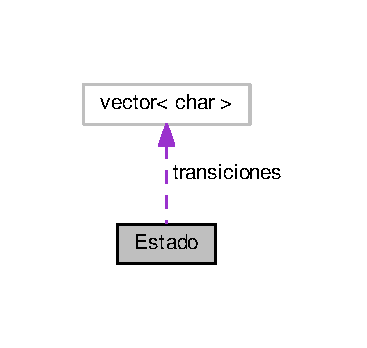
\includegraphics[width=176pt]{classEstado__coll__graph}
\end{center}
\end{figure}
\subsection*{Public Member Functions}
\begin{DoxyCompactItemize}
\item 
\hyperlink{classEstado_aa956f333e0d0b9c54bc8c94055966ea2}{Estado} ()
\item 
\hyperlink{classEstado_a8bb18423eb811e665d831fcaeb0ccf70}{$\sim$\+Estado} ()
\item 
void \hyperlink{classEstado_a1e874111cfafc68c6ab39c7dad5a43a4}{set\+\_\+id} (char)
\item 
void \hyperlink{classEstado_a62752c6851c3c7120f7eabbef45f5dc5}{set\+\_\+id\+\_\+rep} (char)
\item 
void \hyperlink{classEstado_a583f82e7e7a75aa736b6f343dd34485a}{set\+\_\+tipo} (int)
\item 
void \hyperlink{classEstado_aff91838681991dd981d8ba044d0f81e6}{set\+\_\+num\+\_\+trans} (int)
\item 
void \hyperlink{classEstado_a81a3a7a9f2375f593658fb5fff25e5d9}{set\+\_\+trans} (char)
\item 
void \hyperlink{classEstado_a5a151aa6aa1c461b9c7ef1766e3af6ea}{set\+\_\+id\+\_\+conj} (char)
\item 
void \hyperlink{classEstado_a621930abb9101a531e0661a0d15d8bc8}{set\+\_\+impreso} (bool)
\item 
char \hyperlink{classEstado_a49e86800510d41bf2305f12e06e9b643}{get\+\_\+id} ()
\item 
char \hyperlink{classEstado_a4b4836f8937ceaf9f80bf78b31b0d03a}{get\+\_\+id\+\_\+rep} ()
\item 
int \hyperlink{classEstado_a8c7b58bbc9be55203df242465495d9e2}{get\+\_\+tipo} ()
\item 
int \hyperlink{classEstado_a3d4cf6c9cc162a55a2e1ff2e68fd06db}{get\+\_\+num\+\_\+trans} ()
\item 
char \hyperlink{classEstado_a71ea0a4f4cc0258b70165edc36fa2746}{get\+\_\+trans} (int)
\item 
char \hyperlink{classEstado_a1104ea1ad4ea5e68604dd3d76801e6d6}{get\+\_\+id\+\_\+conj} ()
\item 
bool \hyperlink{classEstado_a0f151c7dfe2c751b1a287e137cd96a28}{get\+\_\+impreso} ()
\item 
void \hyperlink{classEstado_a716a68e7ec56b17040b1acbd7e66f538}{cambia\+\_\+trans} (int pos, char id)
\end{DoxyCompactItemize}
\subsection*{Private Attributes}
\begin{DoxyCompactItemize}
\item 
char \hyperlink{classEstado_a49403b58257e25d5239b9c2f9889eec3}{id\+\_\+est}
\item 
char \hyperlink{classEstado_a0633bc8eafa25dfc8bd454b1ae81f49f}{id\+\_\+rep}
\item 
int \hyperlink{classEstado_aaa56d22447e452e34f681fb4db2861a0}{tipe\+\_\+est}
\item 
int \hyperlink{classEstado_a830f36351fa698f5e6f644f6a7c63963}{num\+\_\+trans}
\item 
bool \hyperlink{classEstado_af9ae48b2e90b70ab17b8c88d8663144e}{impreso}
\item 
vector$<$ char $>$ \hyperlink{classEstado_a207caa56f6fea708339cf115f34cfed5}{transiciones}
\item 
int \hyperlink{classEstado_ac3143590b8bb505b4a1b47d1295bbb67}{id\+\_\+conj}
\end{DoxyCompactItemize}


\subsection{Constructor \& Destructor Documentation}
\index{Estado@{Estado}!Estado@{Estado}}
\index{Estado@{Estado}!Estado@{Estado}}
\subsubsection[{\texorpdfstring{Estado()}{Estado()}}]{\setlength{\rightskip}{0pt plus 5cm}Estado\+::\+Estado (
\begin{DoxyParamCaption}
{}
\end{DoxyParamCaption}
)}\hypertarget{classEstado_aa956f333e0d0b9c54bc8c94055966ea2}{}\label{classEstado_aa956f333e0d0b9c54bc8c94055966ea2}
\index{Estado@{Estado}!````~Estado@{$\sim$\+Estado}}
\index{````~Estado@{$\sim$\+Estado}!Estado@{Estado}}
\subsubsection[{\texorpdfstring{$\sim$\+Estado()}{~Estado()}}]{\setlength{\rightskip}{0pt plus 5cm}Estado\+::$\sim$\+Estado (
\begin{DoxyParamCaption}
{}
\end{DoxyParamCaption}
)}\hypertarget{classEstado_a8bb18423eb811e665d831fcaeb0ccf70}{}\label{classEstado_a8bb18423eb811e665d831fcaeb0ccf70}


\subsection{Member Function Documentation}
\index{Estado@{Estado}!cambia\+\_\+trans@{cambia\+\_\+trans}}
\index{cambia\+\_\+trans@{cambia\+\_\+trans}!Estado@{Estado}}
\subsubsection[{\texorpdfstring{cambia\+\_\+trans(int pos, char id)}{cambia_trans(int pos, char id)}}]{\setlength{\rightskip}{0pt plus 5cm}void Estado\+::cambia\+\_\+trans (
\begin{DoxyParamCaption}
\item[{int}]{pos, }
\item[{char}]{id}
\end{DoxyParamCaption}
)}\hypertarget{classEstado_a716a68e7ec56b17040b1acbd7e66f538}{}\label{classEstado_a716a68e7ec56b17040b1acbd7e66f538}
\index{Estado@{Estado}!get\+\_\+id@{get\+\_\+id}}
\index{get\+\_\+id@{get\+\_\+id}!Estado@{Estado}}
\subsubsection[{\texorpdfstring{get\+\_\+id()}{get_id()}}]{\setlength{\rightskip}{0pt plus 5cm}char Estado\+::get\+\_\+id (
\begin{DoxyParamCaption}
{}
\end{DoxyParamCaption}
)}\hypertarget{classEstado_a49e86800510d41bf2305f12e06e9b643}{}\label{classEstado_a49e86800510d41bf2305f12e06e9b643}
\index{Estado@{Estado}!get\+\_\+id\+\_\+conj@{get\+\_\+id\+\_\+conj}}
\index{get\+\_\+id\+\_\+conj@{get\+\_\+id\+\_\+conj}!Estado@{Estado}}
\subsubsection[{\texorpdfstring{get\+\_\+id\+\_\+conj()}{get_id_conj()}}]{\setlength{\rightskip}{0pt plus 5cm}char Estado\+::get\+\_\+id\+\_\+conj (
\begin{DoxyParamCaption}
{}
\end{DoxyParamCaption}
)}\hypertarget{classEstado_a1104ea1ad4ea5e68604dd3d76801e6d6}{}\label{classEstado_a1104ea1ad4ea5e68604dd3d76801e6d6}
\index{Estado@{Estado}!get\+\_\+id\+\_\+rep@{get\+\_\+id\+\_\+rep}}
\index{get\+\_\+id\+\_\+rep@{get\+\_\+id\+\_\+rep}!Estado@{Estado}}
\subsubsection[{\texorpdfstring{get\+\_\+id\+\_\+rep()}{get_id_rep()}}]{\setlength{\rightskip}{0pt plus 5cm}char Estado\+::get\+\_\+id\+\_\+rep (
\begin{DoxyParamCaption}
{}
\end{DoxyParamCaption}
)}\hypertarget{classEstado_a4b4836f8937ceaf9f80bf78b31b0d03a}{}\label{classEstado_a4b4836f8937ceaf9f80bf78b31b0d03a}
\index{Estado@{Estado}!get\+\_\+impreso@{get\+\_\+impreso}}
\index{get\+\_\+impreso@{get\+\_\+impreso}!Estado@{Estado}}
\subsubsection[{\texorpdfstring{get\+\_\+impreso()}{get_impreso()}}]{\setlength{\rightskip}{0pt plus 5cm}bool Estado\+::get\+\_\+impreso (
\begin{DoxyParamCaption}
{}
\end{DoxyParamCaption}
)}\hypertarget{classEstado_a0f151c7dfe2c751b1a287e137cd96a28}{}\label{classEstado_a0f151c7dfe2c751b1a287e137cd96a28}
\index{Estado@{Estado}!get\+\_\+num\+\_\+trans@{get\+\_\+num\+\_\+trans}}
\index{get\+\_\+num\+\_\+trans@{get\+\_\+num\+\_\+trans}!Estado@{Estado}}
\subsubsection[{\texorpdfstring{get\+\_\+num\+\_\+trans()}{get_num_trans()}}]{\setlength{\rightskip}{0pt plus 5cm}int Estado\+::get\+\_\+num\+\_\+trans (
\begin{DoxyParamCaption}
{}
\end{DoxyParamCaption}
)}\hypertarget{classEstado_a3d4cf6c9cc162a55a2e1ff2e68fd06db}{}\label{classEstado_a3d4cf6c9cc162a55a2e1ff2e68fd06db}
\index{Estado@{Estado}!get\+\_\+tipo@{get\+\_\+tipo}}
\index{get\+\_\+tipo@{get\+\_\+tipo}!Estado@{Estado}}
\subsubsection[{\texorpdfstring{get\+\_\+tipo()}{get_tipo()}}]{\setlength{\rightskip}{0pt plus 5cm}int Estado\+::get\+\_\+tipo (
\begin{DoxyParamCaption}
{}
\end{DoxyParamCaption}
)}\hypertarget{classEstado_a8c7b58bbc9be55203df242465495d9e2}{}\label{classEstado_a8c7b58bbc9be55203df242465495d9e2}
\index{Estado@{Estado}!get\+\_\+trans@{get\+\_\+trans}}
\index{get\+\_\+trans@{get\+\_\+trans}!Estado@{Estado}}
\subsubsection[{\texorpdfstring{get\+\_\+trans(int)}{get_trans(int)}}]{\setlength{\rightskip}{0pt plus 5cm}char Estado\+::get\+\_\+trans (
\begin{DoxyParamCaption}
\item[{int}]{i}
\end{DoxyParamCaption}
)}\hypertarget{classEstado_a71ea0a4f4cc0258b70165edc36fa2746}{}\label{classEstado_a71ea0a4f4cc0258b70165edc36fa2746}
\index{Estado@{Estado}!set\+\_\+id@{set\+\_\+id}}
\index{set\+\_\+id@{set\+\_\+id}!Estado@{Estado}}
\subsubsection[{\texorpdfstring{set\+\_\+id(char)}{set_id(char)}}]{\setlength{\rightskip}{0pt plus 5cm}void Estado\+::set\+\_\+id (
\begin{DoxyParamCaption}
\item[{char}]{x}
\end{DoxyParamCaption}
)}\hypertarget{classEstado_a1e874111cfafc68c6ab39c7dad5a43a4}{}\label{classEstado_a1e874111cfafc68c6ab39c7dad5a43a4}
\index{Estado@{Estado}!set\+\_\+id\+\_\+conj@{set\+\_\+id\+\_\+conj}}
\index{set\+\_\+id\+\_\+conj@{set\+\_\+id\+\_\+conj}!Estado@{Estado}}
\subsubsection[{\texorpdfstring{set\+\_\+id\+\_\+conj(char)}{set_id_conj(char)}}]{\setlength{\rightskip}{0pt plus 5cm}void Estado\+::set\+\_\+id\+\_\+conj (
\begin{DoxyParamCaption}
\item[{char}]{x}
\end{DoxyParamCaption}
)}\hypertarget{classEstado_a5a151aa6aa1c461b9c7ef1766e3af6ea}{}\label{classEstado_a5a151aa6aa1c461b9c7ef1766e3af6ea}
\index{Estado@{Estado}!set\+\_\+id\+\_\+rep@{set\+\_\+id\+\_\+rep}}
\index{set\+\_\+id\+\_\+rep@{set\+\_\+id\+\_\+rep}!Estado@{Estado}}
\subsubsection[{\texorpdfstring{set\+\_\+id\+\_\+rep(char)}{set_id_rep(char)}}]{\setlength{\rightskip}{0pt plus 5cm}void Estado\+::set\+\_\+id\+\_\+rep (
\begin{DoxyParamCaption}
\item[{char}]{x}
\end{DoxyParamCaption}
)}\hypertarget{classEstado_a62752c6851c3c7120f7eabbef45f5dc5}{}\label{classEstado_a62752c6851c3c7120f7eabbef45f5dc5}
\index{Estado@{Estado}!set\+\_\+impreso@{set\+\_\+impreso}}
\index{set\+\_\+impreso@{set\+\_\+impreso}!Estado@{Estado}}
\subsubsection[{\texorpdfstring{set\+\_\+impreso(bool)}{set_impreso(bool)}}]{\setlength{\rightskip}{0pt plus 5cm}void Estado\+::set\+\_\+impreso (
\begin{DoxyParamCaption}
\item[{bool}]{x}
\end{DoxyParamCaption}
)}\hypertarget{classEstado_a621930abb9101a531e0661a0d15d8bc8}{}\label{classEstado_a621930abb9101a531e0661a0d15d8bc8}
\index{Estado@{Estado}!set\+\_\+num\+\_\+trans@{set\+\_\+num\+\_\+trans}}
\index{set\+\_\+num\+\_\+trans@{set\+\_\+num\+\_\+trans}!Estado@{Estado}}
\subsubsection[{\texorpdfstring{set\+\_\+num\+\_\+trans(int)}{set_num_trans(int)}}]{\setlength{\rightskip}{0pt plus 5cm}void Estado\+::set\+\_\+num\+\_\+trans (
\begin{DoxyParamCaption}
\item[{int}]{x}
\end{DoxyParamCaption}
)}\hypertarget{classEstado_aff91838681991dd981d8ba044d0f81e6}{}\label{classEstado_aff91838681991dd981d8ba044d0f81e6}
\index{Estado@{Estado}!set\+\_\+tipo@{set\+\_\+tipo}}
\index{set\+\_\+tipo@{set\+\_\+tipo}!Estado@{Estado}}
\subsubsection[{\texorpdfstring{set\+\_\+tipo(int)}{set_tipo(int)}}]{\setlength{\rightskip}{0pt plus 5cm}void Estado\+::set\+\_\+tipo (
\begin{DoxyParamCaption}
\item[{int}]{x}
\end{DoxyParamCaption}
)}\hypertarget{classEstado_a583f82e7e7a75aa736b6f343dd34485a}{}\label{classEstado_a583f82e7e7a75aa736b6f343dd34485a}
\index{Estado@{Estado}!set\+\_\+trans@{set\+\_\+trans}}
\index{set\+\_\+trans@{set\+\_\+trans}!Estado@{Estado}}
\subsubsection[{\texorpdfstring{set\+\_\+trans(char)}{set_trans(char)}}]{\setlength{\rightskip}{0pt plus 5cm}void Estado\+::set\+\_\+trans (
\begin{DoxyParamCaption}
\item[{char}]{sig}
\end{DoxyParamCaption}
)}\hypertarget{classEstado_a81a3a7a9f2375f593658fb5fff25e5d9}{}\label{classEstado_a81a3a7a9f2375f593658fb5fff25e5d9}


\subsection{Member Data Documentation}
\index{Estado@{Estado}!id\+\_\+conj@{id\+\_\+conj}}
\index{id\+\_\+conj@{id\+\_\+conj}!Estado@{Estado}}
\subsubsection[{\texorpdfstring{id\+\_\+conj}{id_conj}}]{\setlength{\rightskip}{0pt plus 5cm}int Estado\+::id\+\_\+conj\hspace{0.3cm}{\ttfamily [private]}}\hypertarget{classEstado_ac3143590b8bb505b4a1b47d1295bbb67}{}\label{classEstado_ac3143590b8bb505b4a1b47d1295bbb67}
\index{Estado@{Estado}!id\+\_\+est@{id\+\_\+est}}
\index{id\+\_\+est@{id\+\_\+est}!Estado@{Estado}}
\subsubsection[{\texorpdfstring{id\+\_\+est}{id_est}}]{\setlength{\rightskip}{0pt plus 5cm}char Estado\+::id\+\_\+est\hspace{0.3cm}{\ttfamily [private]}}\hypertarget{classEstado_a49403b58257e25d5239b9c2f9889eec3}{}\label{classEstado_a49403b58257e25d5239b9c2f9889eec3}
\index{Estado@{Estado}!id\+\_\+rep@{id\+\_\+rep}}
\index{id\+\_\+rep@{id\+\_\+rep}!Estado@{Estado}}
\subsubsection[{\texorpdfstring{id\+\_\+rep}{id_rep}}]{\setlength{\rightskip}{0pt plus 5cm}char Estado\+::id\+\_\+rep\hspace{0.3cm}{\ttfamily [private]}}\hypertarget{classEstado_a0633bc8eafa25dfc8bd454b1ae81f49f}{}\label{classEstado_a0633bc8eafa25dfc8bd454b1ae81f49f}
\index{Estado@{Estado}!impreso@{impreso}}
\index{impreso@{impreso}!Estado@{Estado}}
\subsubsection[{\texorpdfstring{impreso}{impreso}}]{\setlength{\rightskip}{0pt plus 5cm}bool Estado\+::impreso\hspace{0.3cm}{\ttfamily [private]}}\hypertarget{classEstado_af9ae48b2e90b70ab17b8c88d8663144e}{}\label{classEstado_af9ae48b2e90b70ab17b8c88d8663144e}
\index{Estado@{Estado}!num\+\_\+trans@{num\+\_\+trans}}
\index{num\+\_\+trans@{num\+\_\+trans}!Estado@{Estado}}
\subsubsection[{\texorpdfstring{num\+\_\+trans}{num_trans}}]{\setlength{\rightskip}{0pt plus 5cm}int Estado\+::num\+\_\+trans\hspace{0.3cm}{\ttfamily [private]}}\hypertarget{classEstado_a830f36351fa698f5e6f644f6a7c63963}{}\label{classEstado_a830f36351fa698f5e6f644f6a7c63963}
\index{Estado@{Estado}!tipe\+\_\+est@{tipe\+\_\+est}}
\index{tipe\+\_\+est@{tipe\+\_\+est}!Estado@{Estado}}
\subsubsection[{\texorpdfstring{tipe\+\_\+est}{tipe_est}}]{\setlength{\rightskip}{0pt plus 5cm}int Estado\+::tipe\+\_\+est\hspace{0.3cm}{\ttfamily [private]}}\hypertarget{classEstado_aaa56d22447e452e34f681fb4db2861a0}{}\label{classEstado_aaa56d22447e452e34f681fb4db2861a0}
\index{Estado@{Estado}!transiciones@{transiciones}}
\index{transiciones@{transiciones}!Estado@{Estado}}
\subsubsection[{\texorpdfstring{transiciones}{transiciones}}]{\setlength{\rightskip}{0pt plus 5cm}vector$<$char$>$ Estado\+::transiciones\hspace{0.3cm}{\ttfamily [private]}}\hypertarget{classEstado_a207caa56f6fea708339cf115f34cfed5}{}\label{classEstado_a207caa56f6fea708339cf115f34cfed5}


The documentation for this class was generated from the following files\+:\begin{DoxyCompactItemize}
\item 
\hyperlink{Estado_8h}{Estado.\+h}\item 
\hyperlink{Estado_8cpp}{Estado.\+cpp}\end{DoxyCompactItemize}

\chapter{File Documentation}
\hypertarget{CAplicacion_8cpp}{}\section{C\+Aplicacion.\+cpp File Reference}
\label{CAplicacion_8cpp}\index{C\+Aplicacion.\+cpp@{C\+Aplicacion.\+cpp}}
{\ttfamily \#include \char`\"{}C\+Aplicacion.\+h\char`\"{}}\\*
{\ttfamily \#include \char`\"{}opencv2/imgcodecs.\+hpp\char`\"{}}\\*
{\ttfamily \#include \char`\"{}opencv2/imgproc.\+hpp\char`\"{}}\\*
{\ttfamily \#include \char`\"{}opencv2/opencv.\+hpp\char`\"{}}\\*
{\ttfamily \#include $<$iostream$>$}\\*
Include dependency graph for C\+Aplicacion.\+cpp\+:

\hypertarget{CAplicacion_8h}{}\section{C\+Aplicacion.\+h File Reference}
\label{CAplicacion_8h}\index{C\+Aplicacion.\+h@{C\+Aplicacion.\+h}}
{\ttfamily \#include $<$Qt\+Widgets$>$}\\*
{\ttfamily \#include \char`\"{}C\+Label.\+h\char`\"{}}\\*
{\ttfamily \#include \char`\"{}C\+Line\+Edit.\+h\char`\"{}}\\*
{\ttfamily \#include \char`\"{}C\+Operaciones\+Imagen.\+h\char`\"{}}\\*
{\ttfamily \#include \char`\"{}C\+Panel\+Opciones.\+h\char`\"{}}\\*
Include dependency graph for C\+Aplicacion.\+h\+:
\nopagebreak
\begin{figure}[H]
\begin{center}
\leavevmode
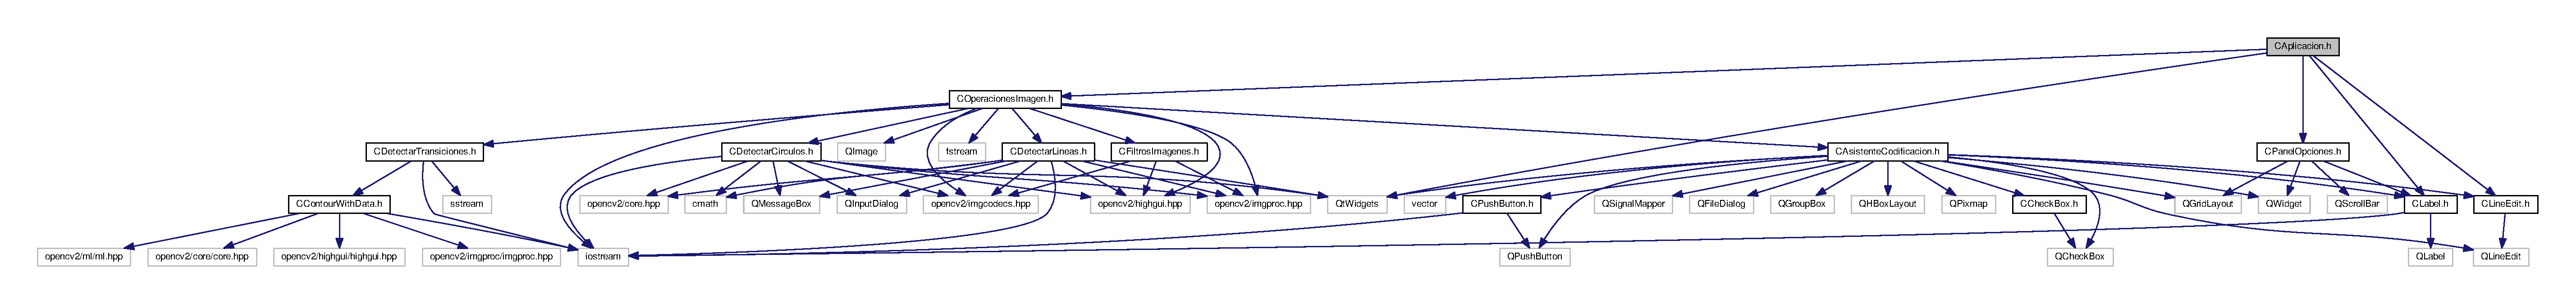
\includegraphics[width=350pt]{CAplicacion_8h__incl}
\end{center}
\end{figure}
This graph shows which files directly or indirectly include this file\+:
\nopagebreak
\begin{figure}[H]
\begin{center}
\leavevmode
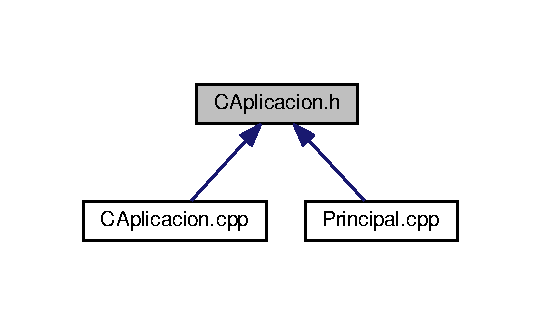
\includegraphics[width=260pt]{CAplicacion_8h__dep__incl}
\end{center}
\end{figure}
\subsection*{Classes}
\begin{DoxyCompactItemize}
\item 
class \hyperlink{classCAplicacion}{C\+Aplicacion}
\begin{DoxyCompactList}\small\item\em Clase Aplicacion con ventana principal de la aplicacion Consta de 3 Paneles. Principal, Opciones e Histograma Si se utiliza la funcionalidad Codificar, ese panel cambia de forma T\+E\+R\+M\+I\+N\+AR. \end{DoxyCompactList}\end{DoxyCompactItemize}

\hypertarget{CAsistenteCodificacion_8cpp}{}\section{C\+Asistente\+Codificacion.\+cpp File Reference}
\label{CAsistenteCodificacion_8cpp}\index{C\+Asistente\+Codificacion.\+cpp@{C\+Asistente\+Codificacion.\+cpp}}
{\ttfamily \#include \char`\"{}C\+Asistente\+Codificacion.\+h\char`\"{}}\\*
{\ttfamily \#include \char`\"{}opencv2/opencv.\+hpp\char`\"{}}\\*
Include dependency graph for C\+Asistente\+Codificacion.\+cpp\+:
% FIG 0

\hypertarget{CAsistenteCodificacion_8h}{}\section{C\+Asistente\+Codificacion.\+h File Reference}
\label{CAsistenteCodificacion_8h}\index{C\+Asistente\+Codificacion.\+h@{C\+Asistente\+Codificacion.\+h}}
{\ttfamily \#include $<$Q\+Widget$>$}\\*
{\ttfamily \#include $<$Q\+Grid\+Layout$>$}\\*
{\ttfamily \#include $<$Q\+Check\+Box$>$}\\*
{\ttfamily \#include $<$Q\+Line\+Edit$>$}\\*
{\ttfamily \#include $<$Q\+Push\+Button$>$}\\*
{\ttfamily \#include $<$vector$>$}\\*
{\ttfamily \#include $<$Q\+Signal\+Mapper$>$}\\*
{\ttfamily \#include $<$Q\+File\+Dialog$>$}\\*
{\ttfamily \#include $<$Qt\+Widgets$>$}\\*
{\ttfamily \#include $<$Q\+Group\+Box$>$}\\*
{\ttfamily \#include $<$Q\+H\+Box\+Layout$>$}\\*
{\ttfamily \#include $<$Q\+Pixmap$>$}\\*
{\ttfamily \#include \char`\"{}C\+Push\+Button.\+h\char`\"{}}\\*
{\ttfamily \#include \char`\"{}C\+Label.\+h\char`\"{}}\\*
{\ttfamily \#include \char`\"{}C\+Line\+Edit.\+h\char`\"{}}\\*
{\ttfamily \#include \char`\"{}C\+Check\+Box.\+h\char`\"{}}\\*
Include dependency graph for C\+Asistente\+Codificacion.\+h\+:
\nopagebreak
\begin{figure}[H]
\begin{center}
\leavevmode
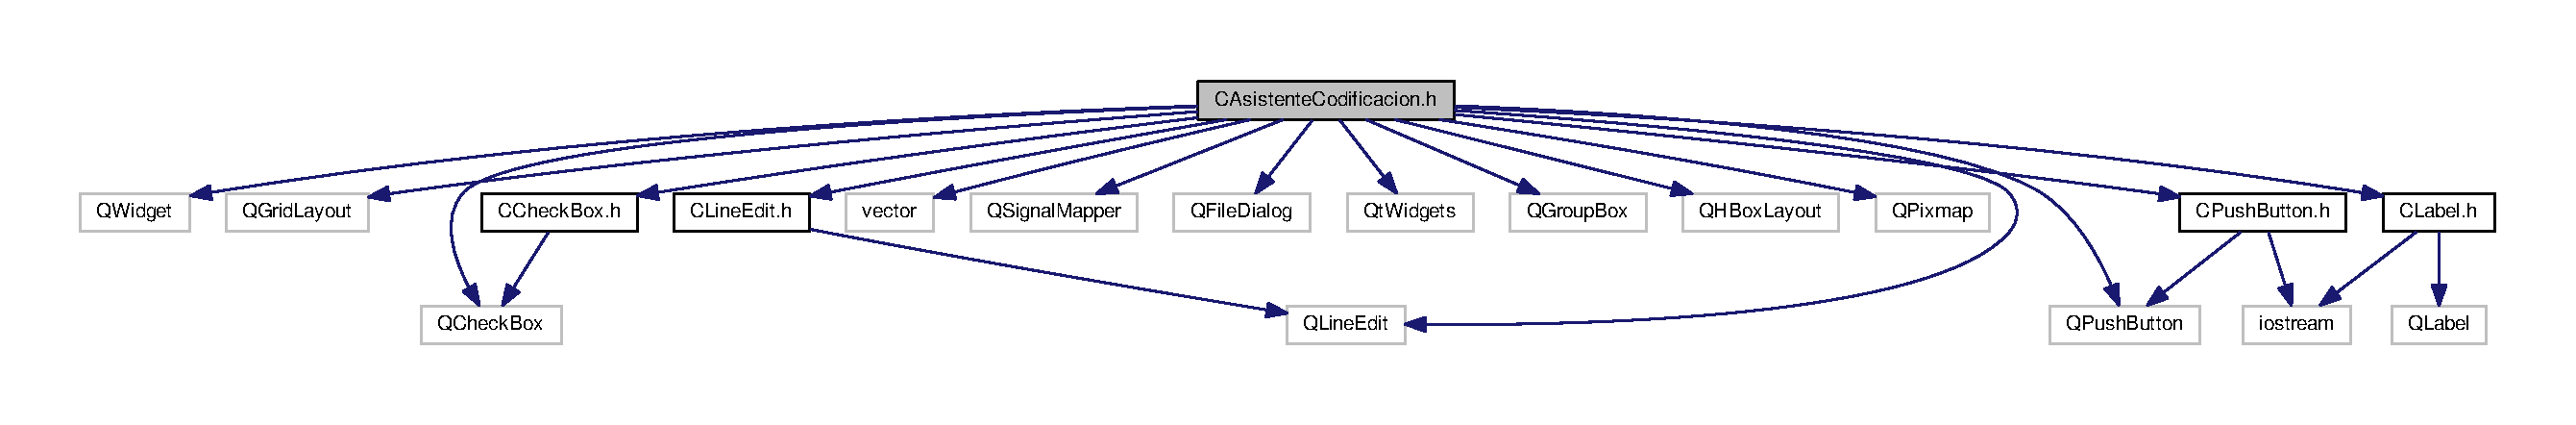
\includegraphics[width=350pt]{CAsistenteCodificacion_8h__incl}
\end{center}
\end{figure}
This graph shows which files directly or indirectly include this file\+:
\nopagebreak
\begin{figure}[H]
\begin{center}
\leavevmode
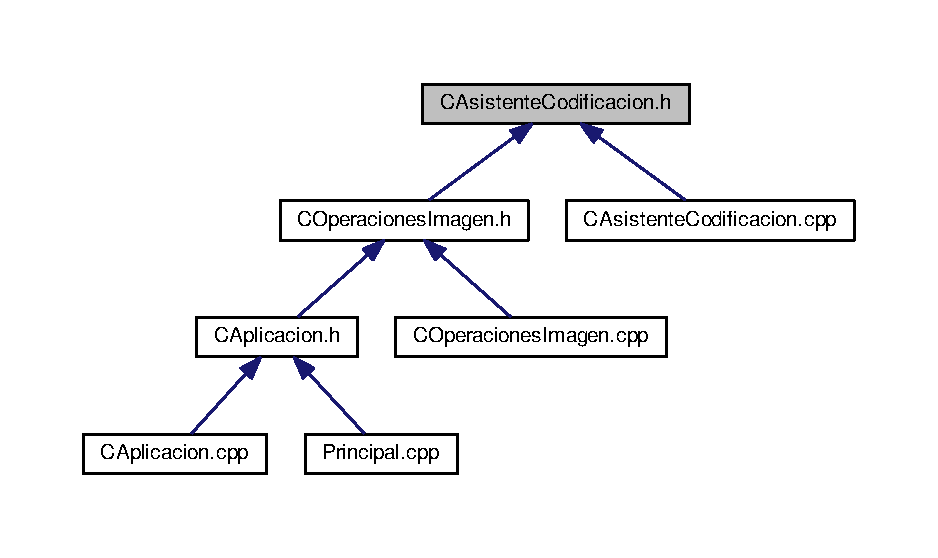
\includegraphics[width=350pt]{CAsistenteCodificacion_8h__dep__incl}
\end{center}
\end{figure}
\subsection*{Classes}
\begin{DoxyCompactItemize}
\item 
class \hyperlink{classCAsistenteCodificacion}{C\+Asistente\+Codificacion}
\begin{DoxyCompactList}\small\item\em Clase asistente de la codificacion. Utilizada al Procesar o Codificar una Imagen para confirmar que todo es correcto antes de guardarlo en un fichero. \end{DoxyCompactList}\end{DoxyCompactItemize}

\hypertarget{CCheckBox_8cpp}{}\section{C\+Check\+Box.\+cpp File Reference}
\label{CCheckBox_8cpp}\index{C\+Check\+Box.\+cpp@{C\+Check\+Box.\+cpp}}
{\ttfamily \#include \char`\"{}C\+Check\+Box.\+h\char`\"{}}\\*
Include dependency graph for C\+Check\+Box.\+cpp\+:
% FIG 0

\hypertarget{CCheckBox_8h}{}\section{C\+Check\+Box.\+h File Reference}
\label{CCheckBox_8h}\index{C\+Check\+Box.\+h@{C\+Check\+Box.\+h}}
{\ttfamily \#include $<$Q\+Check\+Box$>$}\\*
Include dependency graph for C\+Check\+Box.\+h\+:\nopagebreak
\begin{figure}[H]
\begin{center}
\leavevmode
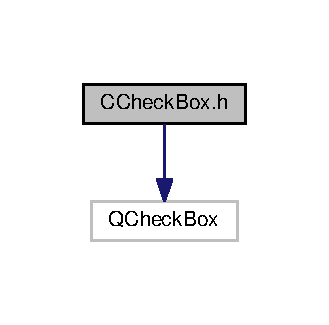
\includegraphics[width=158pt]{CCheckBox_8h__incl}
\end{center}
\end{figure}
This graph shows which files directly or indirectly include this file\+:\nopagebreak
\begin{figure}[H]
\begin{center}
\leavevmode
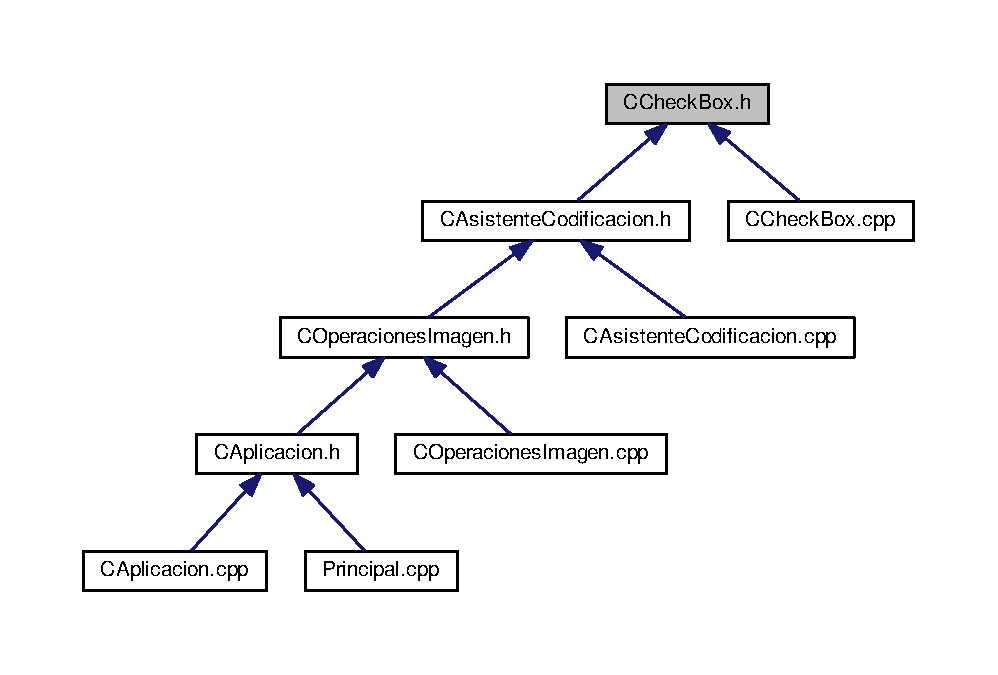
\includegraphics[width=350pt]{CCheckBox_8h__dep__incl}
\end{center}
\end{figure}
\subsection*{Classes}
\begin{DoxyCompactItemize}
\item 
class \hyperlink{classCCheckBox}{C\+Check\+Box}
\begin{DoxyCompactList}\small\item\em Clase heredada de \textquotesingle{}Q\+Check\+Box\textquotesingle{} que aplica un estilo determinado a este tipo de container. \end{DoxyCompactList}\end{DoxyCompactItemize}

\hypertarget{CContourWithData_8cpp}{}\section{C\+Contour\+With\+Data.\+cpp File Reference}
\label{CContourWithData_8cpp}\index{C\+Contour\+With\+Data.\+cpp@{C\+Contour\+With\+Data.\+cpp}}
{\ttfamily \#include \char`\"{}C\+Contour\+With\+Data.\+h\char`\"{}}\\*
Include dependency graph for C\+Contour\+With\+Data.\+cpp\+:\nopagebreak
\begin{figure}[H]
\begin{center}
\leavevmode
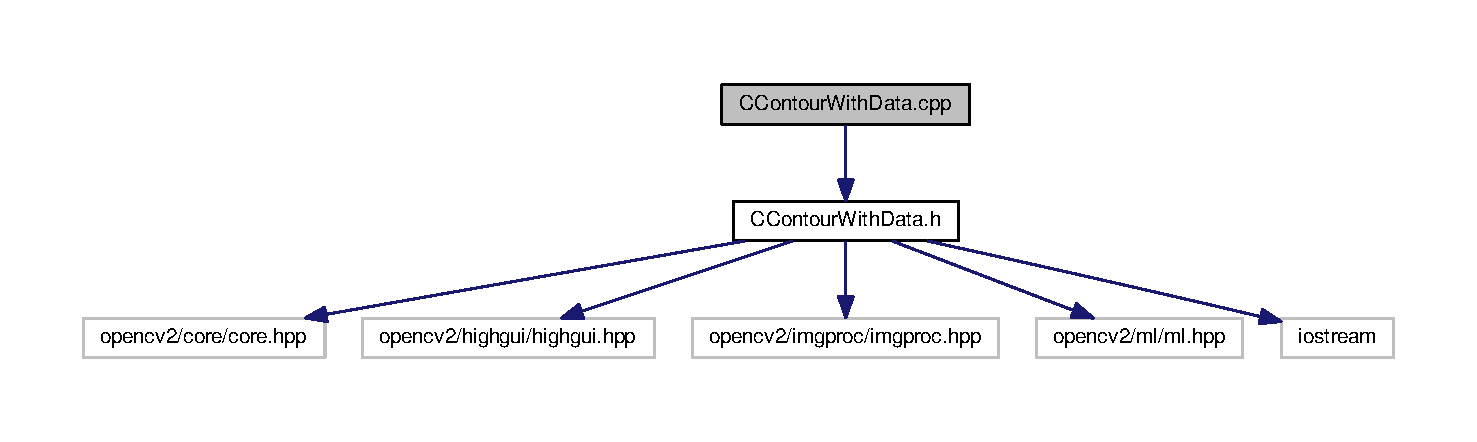
\includegraphics[width=350pt]{CContourWithData_8cpp__incl}
\end{center}
\end{figure}

\hypertarget{CContourWithData_8h}{}\section{C\+Contour\+With\+Data.\+h File Reference}
\label{CContourWithData_8h}\index{C\+Contour\+With\+Data.\+h@{C\+Contour\+With\+Data.\+h}}
{\ttfamily \#include $<$opencv2/core/core.\+hpp$>$}\\*
{\ttfamily \#include $<$opencv2/highgui/highgui.\+hpp$>$}\\*
{\ttfamily \#include $<$opencv2/imgproc/imgproc.\+hpp$>$}\\*
{\ttfamily \#include $<$opencv2/ml/ml.\+hpp$>$}\\*
{\ttfamily \#include $<$iostream$>$}\\*
Include dependency graph for C\+Contour\+With\+Data.\+h\+:
% FIG 0
This graph shows which files directly or indirectly include this file\+:
% FIG 1
\subsection*{Classes}
\begin{DoxyCompactItemize}
\item 
class \hyperlink{classCContourWithData}{C\+Contour\+With\+Data}
\end{DoxyCompactItemize}
\subsection*{Macros}
\begin{DoxyCompactItemize}
\item 
\#define \hyperlink{CContourWithData_8h_af2984e0165183f2b9f9414e7e713b92a}{M\+I\+N\+\_\+\+C\+O\+N\+T\+O\+U\+R\+\_\+\+A\+R\+EA}~100
\end{DoxyCompactItemize}


\subsection{Macro Definition Documentation}
\index{C\+Contour\+With\+Data.\+h@{C\+Contour\+With\+Data.\+h}!M\+I\+N\+\_\+\+C\+O\+N\+T\+O\+U\+R\+\_\+\+A\+R\+EA@{M\+I\+N\+\_\+\+C\+O\+N\+T\+O\+U\+R\+\_\+\+A\+R\+EA}}
\index{M\+I\+N\+\_\+\+C\+O\+N\+T\+O\+U\+R\+\_\+\+A\+R\+EA@{M\+I\+N\+\_\+\+C\+O\+N\+T\+O\+U\+R\+\_\+\+A\+R\+EA}!C\+Contour\+With\+Data.\+h@{C\+Contour\+With\+Data.\+h}}
\subsubsection[{\texorpdfstring{M\+I\+N\+\_\+\+C\+O\+N\+T\+O\+U\+R\+\_\+\+A\+R\+EA}{MIN_CONTOUR_AREA}}]{\setlength{\rightskip}{0pt plus 5cm}\#define M\+I\+N\+\_\+\+C\+O\+N\+T\+O\+U\+R\+\_\+\+A\+R\+EA~100}\hypertarget{CContourWithData_8h_af2984e0165183f2b9f9414e7e713b92a}{}\label{CContourWithData_8h_af2984e0165183f2b9f9414e7e713b92a}

\hypertarget{CDetectarCirculos_8cpp}{}\section{C\+Detectar\+Circulos.\+cpp File Reference}
\label{CDetectarCirculos_8cpp}\index{C\+Detectar\+Circulos.\+cpp@{C\+Detectar\+Circulos.\+cpp}}
{\ttfamily \#include \char`\"{}C\+Detectar\+Circulos.\+h\char`\"{}}\\*
Include dependency graph for C\+Detectar\+Circulos.\+cpp\+:\nopagebreak
\begin{figure}[H]
\begin{center}
\leavevmode
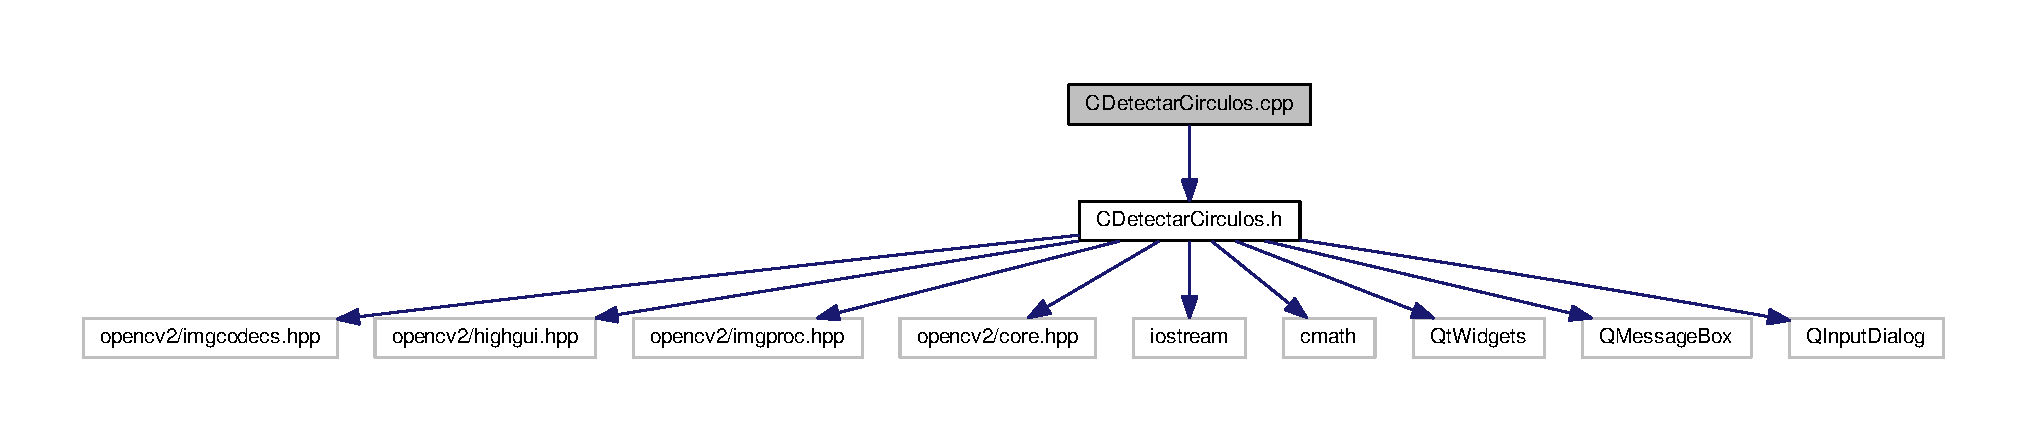
\includegraphics[width=350pt]{CDetectarCirculos_8cpp__incl}
\end{center}
\end{figure}

\hypertarget{CDetectarCirculos_8h}{}\section{C\+Detectar\+Circulos.\+h File Reference}
\label{CDetectarCirculos_8h}\index{C\+Detectar\+Circulos.\+h@{C\+Detectar\+Circulos.\+h}}
{\ttfamily \#include \char`\"{}opencv2/imgcodecs.\+hpp\char`\"{}}\\*
{\ttfamily \#include \char`\"{}opencv2/highgui.\+hpp\char`\"{}}\\*
{\ttfamily \#include \char`\"{}opencv2/imgproc.\+hpp\char`\"{}}\\*
{\ttfamily \#include \char`\"{}opencv2/core.\+hpp\char`\"{}}\\*
{\ttfamily \#include $<$iostream$>$}\\*
{\ttfamily \#include $<$cmath$>$}\\*
{\ttfamily \#include $<$Qt\+Widgets$>$}\\*
{\ttfamily \#include $<$Q\+Message\+Box$>$}\\*
{\ttfamily \#include $<$Q\+Input\+Dialog$>$}\\*
Include dependency graph for C\+Detectar\+Circulos.\+h\+:\nopagebreak
\begin{figure}[H]
\begin{center}
\leavevmode
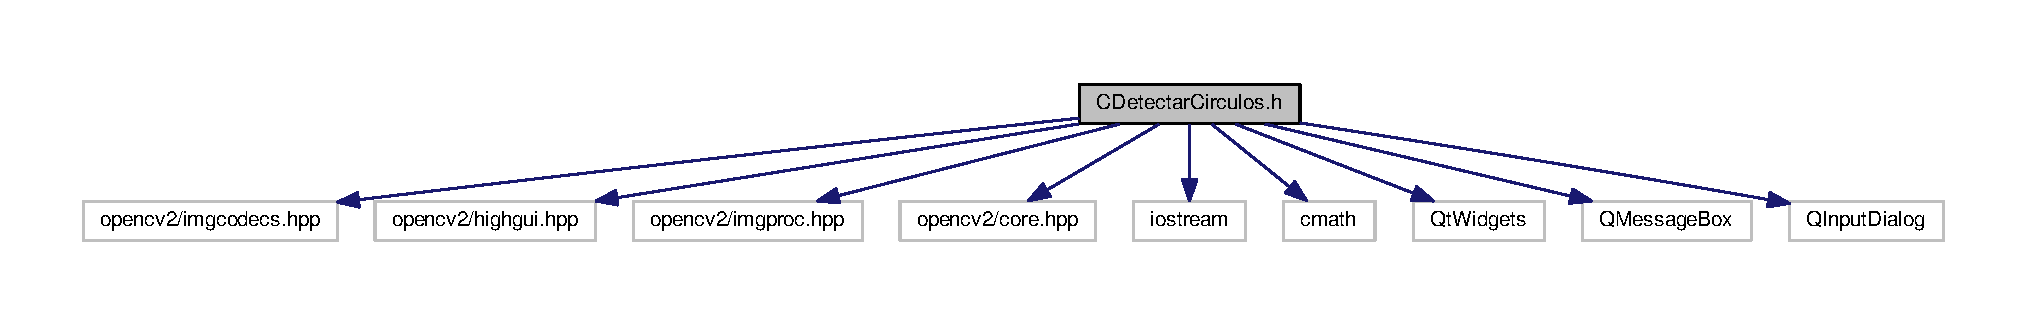
\includegraphics[width=350pt]{CDetectarCirculos_8h__incl}
\end{center}
\end{figure}
This graph shows which files directly or indirectly include this file\+:\nopagebreak
\begin{figure}[H]
\begin{center}
\leavevmode
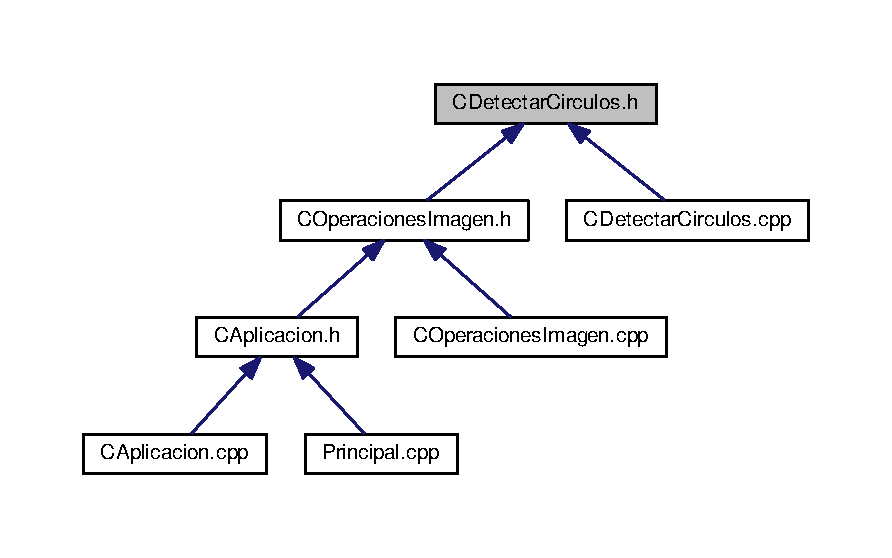
\includegraphics[width=350pt]{CDetectarCirculos_8h__dep__incl}
\end{center}
\end{figure}
\subsection*{Classes}
\begin{DoxyCompactItemize}
\item 
class \hyperlink{classCDetectarCirculo}{C\+Detectar\+Circulo}
\begin{DoxyCompactList}\small\item\em Clase para la deteccion de Circulos Valores por defecto para la deteccion, canny entre 26, 118 y acummulador 45. \end{DoxyCompactList}\end{DoxyCompactItemize}

\hypertarget{CDetectarLineas_8cpp}{}\section{C\+Detectar\+Lineas.\+cpp File Reference}
\label{CDetectarLineas_8cpp}\index{C\+Detectar\+Lineas.\+cpp@{C\+Detectar\+Lineas.\+cpp}}
{\ttfamily \#include \char`\"{}C\+Detectar\+Lineas.\+h\char`\"{}}\\*
Include dependency graph for C\+Detectar\+Lineas.\+cpp\+:\nopagebreak
\begin{figure}[H]
\begin{center}
\leavevmode
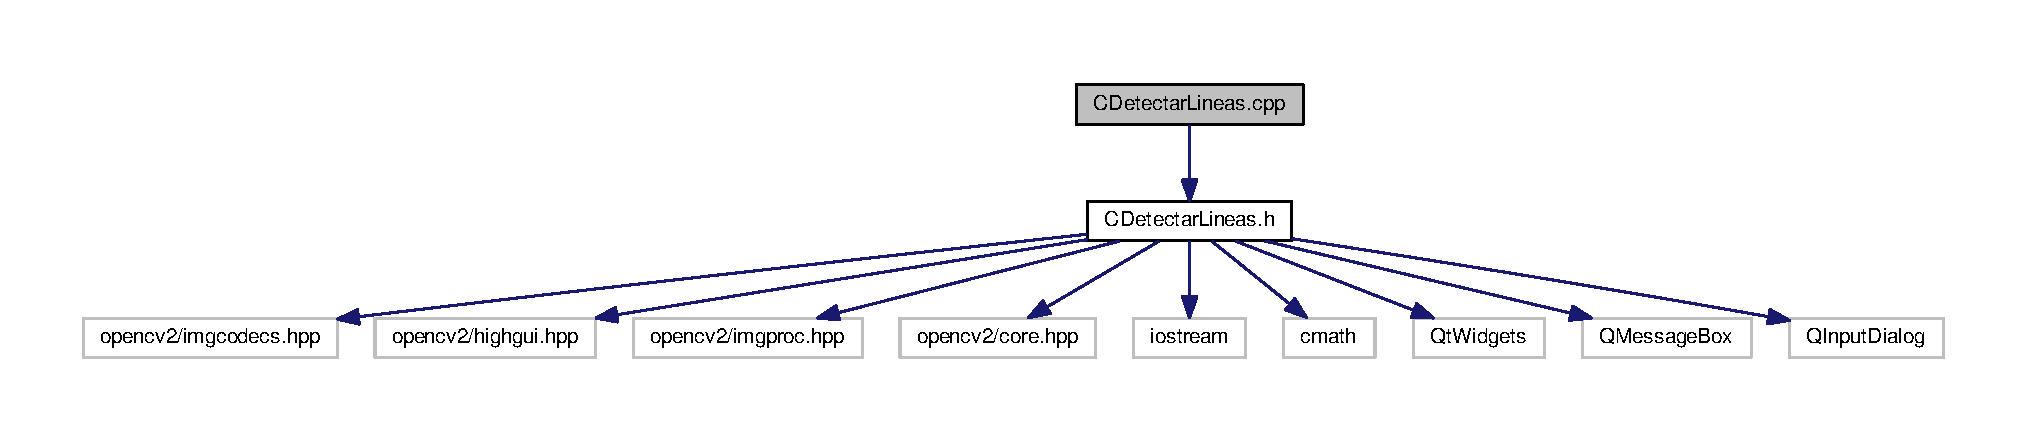
\includegraphics[width=350pt]{CDetectarLineas_8cpp__incl}
\end{center}
\end{figure}

\hypertarget{CDetectarLineas_8h}{}\section{C\+Detectar\+Lineas.\+h File Reference}
\label{CDetectarLineas_8h}\index{C\+Detectar\+Lineas.\+h@{C\+Detectar\+Lineas.\+h}}
{\ttfamily \#include \char`\"{}opencv2/imgcodecs.\+hpp\char`\"{}}\\*
{\ttfamily \#include \char`\"{}opencv2/highgui.\+hpp\char`\"{}}\\*
{\ttfamily \#include \char`\"{}opencv2/imgproc.\+hpp\char`\"{}}\\*
{\ttfamily \#include \char`\"{}opencv2/core.\+hpp\char`\"{}}\\*
{\ttfamily \#include $<$iostream$>$}\\*
{\ttfamily \#include $<$cmath$>$}\\*
{\ttfamily \#include $<$Qt\+Widgets$>$}\\*
{\ttfamily \#include $<$Q\+Message\+Box$>$}\\*
{\ttfamily \#include $<$Q\+Input\+Dialog$>$}\\*
Include dependency graph for C\+Detectar\+Lineas.\+h\+:
% FIG 0
This graph shows which files directly or indirectly include this file\+:
% FIG 1
\subsection*{Classes}
\begin{DoxyCompactItemize}
\item 
class \hyperlink{classCDetectarLineas}{C\+Detectar\+Lineas}
\end{DoxyCompactItemize}
\subsection*{Macros}
\begin{DoxyCompactItemize}
\item 
\#define \hyperlink{CDetectarLineas_8h_a341ac04e22a8d0fa735a902dfdfd8b6e}{D\+I\+S\+T\+A\+N\+C\+I\+A\+P\+I\+X\+E\+L\+P\+R\+I\+N\+C\+I\+P\+AL}~10
\item 
\#define \hyperlink{CDetectarLineas_8h_a78f103953448da00003a8665e5587375}{D\+I\+S\+T\+A\+N\+C\+I\+A\+P\+I\+X\+E\+L\+S\+E\+C\+U\+N\+D\+A\+R\+I\+O\+L\+I\+N\+E\+AS}~30
\end{DoxyCompactItemize}


\subsection{Macro Definition Documentation}
\index{C\+Detectar\+Lineas.\+h@{C\+Detectar\+Lineas.\+h}!D\+I\+S\+T\+A\+N\+C\+I\+A\+P\+I\+X\+E\+L\+P\+R\+I\+N\+C\+I\+P\+AL@{D\+I\+S\+T\+A\+N\+C\+I\+A\+P\+I\+X\+E\+L\+P\+R\+I\+N\+C\+I\+P\+AL}}
\index{D\+I\+S\+T\+A\+N\+C\+I\+A\+P\+I\+X\+E\+L\+P\+R\+I\+N\+C\+I\+P\+AL@{D\+I\+S\+T\+A\+N\+C\+I\+A\+P\+I\+X\+E\+L\+P\+R\+I\+N\+C\+I\+P\+AL}!C\+Detectar\+Lineas.\+h@{C\+Detectar\+Lineas.\+h}}
\subsubsection[{\texorpdfstring{D\+I\+S\+T\+A\+N\+C\+I\+A\+P\+I\+X\+E\+L\+P\+R\+I\+N\+C\+I\+P\+AL}{DISTANCIAPIXELPRINCIPAL}}]{\setlength{\rightskip}{0pt plus 5cm}\#define D\+I\+S\+T\+A\+N\+C\+I\+A\+P\+I\+X\+E\+L\+P\+R\+I\+N\+C\+I\+P\+AL~10}\hypertarget{CDetectarLineas_8h_a341ac04e22a8d0fa735a902dfdfd8b6e}{}\label{CDetectarLineas_8h_a341ac04e22a8d0fa735a902dfdfd8b6e}
\index{C\+Detectar\+Lineas.\+h@{C\+Detectar\+Lineas.\+h}!D\+I\+S\+T\+A\+N\+C\+I\+A\+P\+I\+X\+E\+L\+S\+E\+C\+U\+N\+D\+A\+R\+I\+O\+L\+I\+N\+E\+AS@{D\+I\+S\+T\+A\+N\+C\+I\+A\+P\+I\+X\+E\+L\+S\+E\+C\+U\+N\+D\+A\+R\+I\+O\+L\+I\+N\+E\+AS}}
\index{D\+I\+S\+T\+A\+N\+C\+I\+A\+P\+I\+X\+E\+L\+S\+E\+C\+U\+N\+D\+A\+R\+I\+O\+L\+I\+N\+E\+AS@{D\+I\+S\+T\+A\+N\+C\+I\+A\+P\+I\+X\+E\+L\+S\+E\+C\+U\+N\+D\+A\+R\+I\+O\+L\+I\+N\+E\+AS}!C\+Detectar\+Lineas.\+h@{C\+Detectar\+Lineas.\+h}}
\subsubsection[{\texorpdfstring{D\+I\+S\+T\+A\+N\+C\+I\+A\+P\+I\+X\+E\+L\+S\+E\+C\+U\+N\+D\+A\+R\+I\+O\+L\+I\+N\+E\+AS}{DISTANCIAPIXELSECUNDARIOLINEAS}}]{\setlength{\rightskip}{0pt plus 5cm}\#define D\+I\+S\+T\+A\+N\+C\+I\+A\+P\+I\+X\+E\+L\+S\+E\+C\+U\+N\+D\+A\+R\+I\+O\+L\+I\+N\+E\+AS~30}\hypertarget{CDetectarLineas_8h_a78f103953448da00003a8665e5587375}{}\label{CDetectarLineas_8h_a78f103953448da00003a8665e5587375}

\hypertarget{CDetectarTransiciones_8cpp}{}\section{C\+Detectar\+Transiciones.\+cpp File Reference}
\label{CDetectarTransiciones_8cpp}\index{C\+Detectar\+Transiciones.\+cpp@{C\+Detectar\+Transiciones.\+cpp}}
{\ttfamily \#include \char`\"{}C\+Detectar\+Transiciones.\+h\char`\"{}}\\*
Include dependency graph for C\+Detectar\+Transiciones.\+cpp\+:
\nopagebreak
\begin{figure}[H]
\begin{center}
\leavevmode
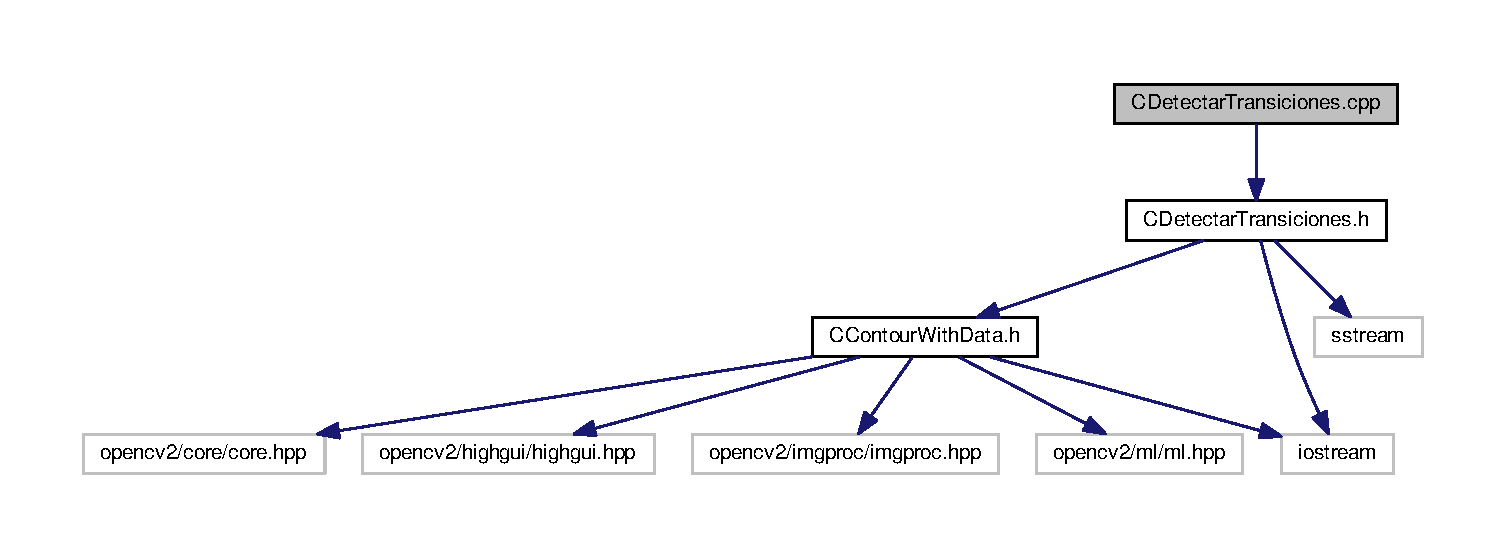
\includegraphics[width=350pt]{CDetectarTransiciones_8cpp__incl}
\end{center}
\end{figure}

\hypertarget{CDetectarTransiciones_8h}{}\section{C\+Detectar\+Transiciones.\+h File Reference}
\label{CDetectarTransiciones_8h}\index{C\+Detectar\+Transiciones.\+h@{C\+Detectar\+Transiciones.\+h}}
{\ttfamily \#include \char`\"{}C\+Contour\+With\+Data.\+h\char`\"{}}\\*
{\ttfamily \#include $<$iostream$>$}\\*
{\ttfamily \#include $<$sstream$>$}\\*
Include dependency graph for C\+Detectar\+Transiciones.\+h\+:\nopagebreak
\begin{figure}[H]
\begin{center}
\leavevmode
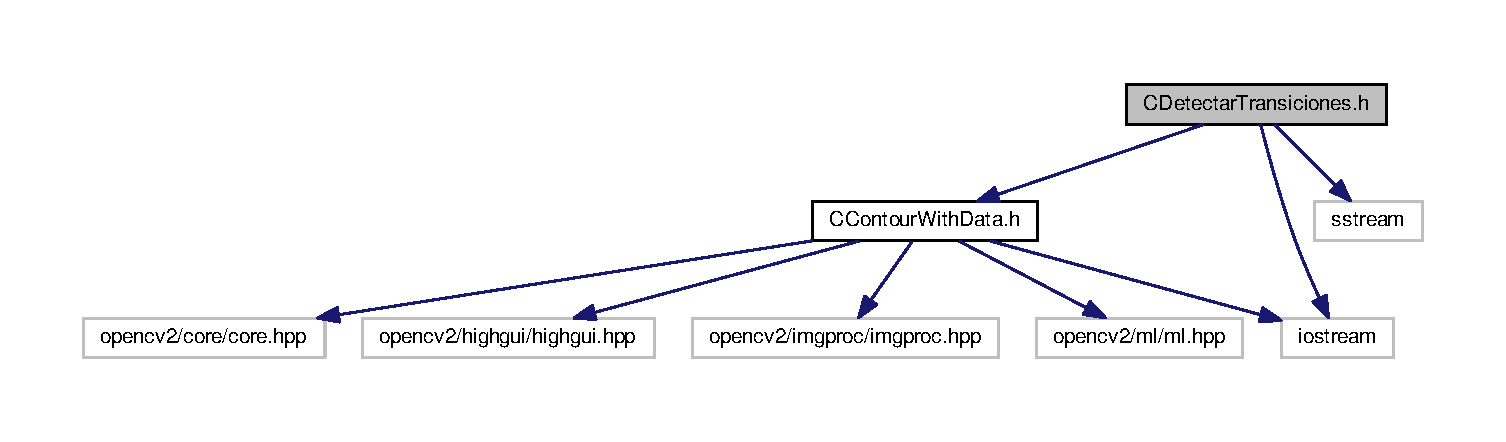
\includegraphics[width=350pt]{CDetectarTransiciones_8h__incl}
\end{center}
\end{figure}
This graph shows which files directly or indirectly include this file\+:\nopagebreak
\begin{figure}[H]
\begin{center}
\leavevmode
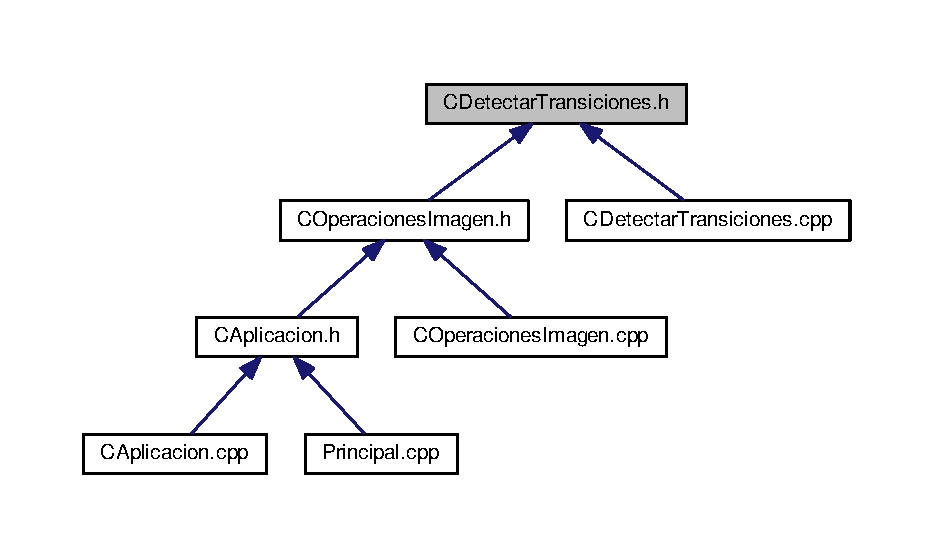
\includegraphics[width=350pt]{CDetectarTransiciones_8h__dep__incl}
\end{center}
\end{figure}
\subsection*{Classes}
\begin{DoxyCompactItemize}
\item 
class \hyperlink{classCDetectarTransiciones}{C\+Detectar\+Transiciones}
\begin{DoxyCompactList}\small\item\em Clase para la dereccion de Transiciones a partir de images.\+xml y classification.\+xml Ambos sacados de Generar\+Clasificador. Proceso de Aprendizaje. \end{DoxyCompactList}\end{DoxyCompactItemize}
\subsection*{Variables}
\begin{DoxyCompactItemize}
\item 
const int \hyperlink{CDetectarTransiciones_8h_a3cc1663820bb978e396a3e56222d2e31}{R\+E\+S\+I\+Z\+E\+D\+\_\+\+I\+M\+A\+G\+E\+\_\+\+W\+I\+D\+TH} = 20
\item 
const int \hyperlink{CDetectarTransiciones_8h_a62612b09bbddc2231deace193108338e}{R\+E\+S\+I\+Z\+E\+D\+\_\+\+I\+M\+A\+G\+E\+\_\+\+H\+E\+I\+G\+HT} = 30
\end{DoxyCompactItemize}


\subsection{Variable Documentation}
\index{C\+Detectar\+Transiciones.\+h@{C\+Detectar\+Transiciones.\+h}!R\+E\+S\+I\+Z\+E\+D\+\_\+\+I\+M\+A\+G\+E\+\_\+\+H\+E\+I\+G\+HT@{R\+E\+S\+I\+Z\+E\+D\+\_\+\+I\+M\+A\+G\+E\+\_\+\+H\+E\+I\+G\+HT}}
\index{R\+E\+S\+I\+Z\+E\+D\+\_\+\+I\+M\+A\+G\+E\+\_\+\+H\+E\+I\+G\+HT@{R\+E\+S\+I\+Z\+E\+D\+\_\+\+I\+M\+A\+G\+E\+\_\+\+H\+E\+I\+G\+HT}!C\+Detectar\+Transiciones.\+h@{C\+Detectar\+Transiciones.\+h}}
\subsubsection[{\texorpdfstring{R\+E\+S\+I\+Z\+E\+D\+\_\+\+I\+M\+A\+G\+E\+\_\+\+H\+E\+I\+G\+HT}{RESIZED_IMAGE_HEIGHT}}]{\setlength{\rightskip}{0pt plus 5cm}const int R\+E\+S\+I\+Z\+E\+D\+\_\+\+I\+M\+A\+G\+E\+\_\+\+H\+E\+I\+G\+HT = 30}\hypertarget{CDetectarTransiciones_8h_a62612b09bbddc2231deace193108338e}{}\label{CDetectarTransiciones_8h_a62612b09bbddc2231deace193108338e}
\index{C\+Detectar\+Transiciones.\+h@{C\+Detectar\+Transiciones.\+h}!R\+E\+S\+I\+Z\+E\+D\+\_\+\+I\+M\+A\+G\+E\+\_\+\+W\+I\+D\+TH@{R\+E\+S\+I\+Z\+E\+D\+\_\+\+I\+M\+A\+G\+E\+\_\+\+W\+I\+D\+TH}}
\index{R\+E\+S\+I\+Z\+E\+D\+\_\+\+I\+M\+A\+G\+E\+\_\+\+W\+I\+D\+TH@{R\+E\+S\+I\+Z\+E\+D\+\_\+\+I\+M\+A\+G\+E\+\_\+\+W\+I\+D\+TH}!C\+Detectar\+Transiciones.\+h@{C\+Detectar\+Transiciones.\+h}}
\subsubsection[{\texorpdfstring{R\+E\+S\+I\+Z\+E\+D\+\_\+\+I\+M\+A\+G\+E\+\_\+\+W\+I\+D\+TH}{RESIZED_IMAGE_WIDTH}}]{\setlength{\rightskip}{0pt plus 5cm}const int R\+E\+S\+I\+Z\+E\+D\+\_\+\+I\+M\+A\+G\+E\+\_\+\+W\+I\+D\+TH = 20}\hypertarget{CDetectarTransiciones_8h_a3cc1663820bb978e396a3e56222d2e31}{}\label{CDetectarTransiciones_8h_a3cc1663820bb978e396a3e56222d2e31}

\hypertarget{CEstadoNFA_8cpp}{}\section{C\+Estado\+N\+F\+A.\+cpp File Reference}
\label{CEstadoNFA_8cpp}\index{C\+Estado\+N\+F\+A.\+cpp@{C\+Estado\+N\+F\+A.\+cpp}}
{\ttfamily \#include \char`\"{}C\+Estado\+N\+F\+A.\+h\char`\"{}}\\*
{\ttfamily \#include $<$iostream$>$}\\*
{\ttfamily \#include $<$vector$>$}\\*
{\ttfamily \#include $<$string$>$}\\*
{\ttfamily \#include $<$stdlib.\+h$>$}\\*
{\ttfamily \#include $<$cstdio$>$}\\*
{\ttfamily \#include $<$stdio.\+h$>$}\\*
{\ttfamily \#include $<$string.\+h$>$}\\*
Include dependency graph for C\+Estado\+N\+F\+A.\+cpp\+:
\nopagebreak
\begin{figure}[H]
\begin{center}
\leavevmode
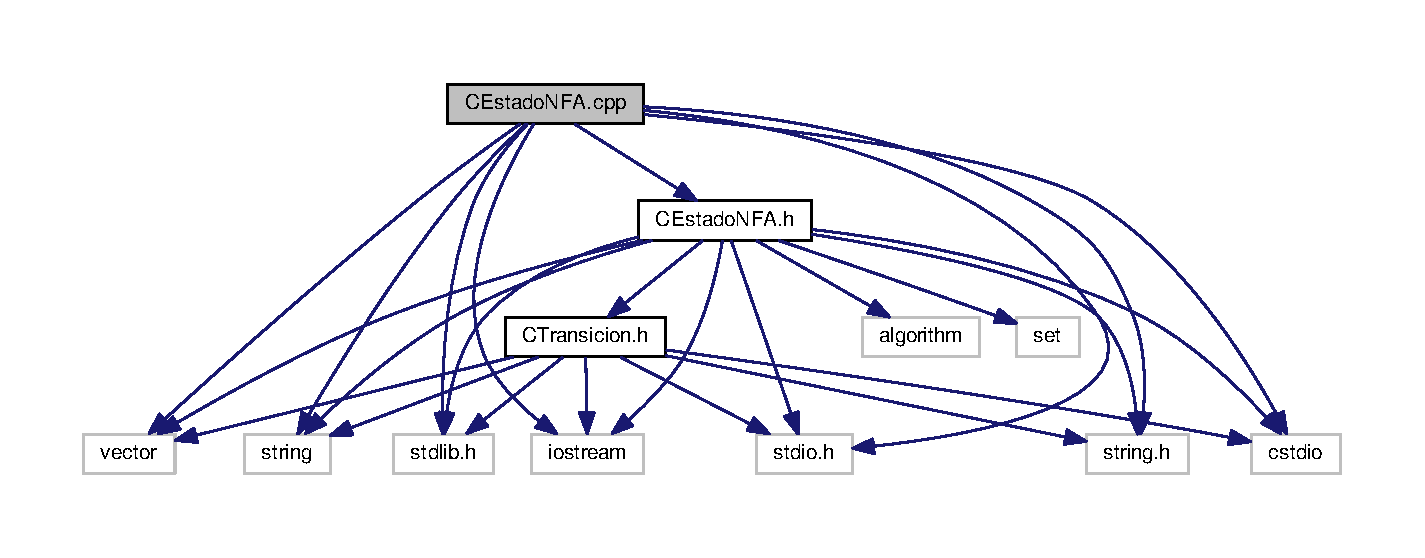
\includegraphics[width=350pt]{CEstadoNFA_8cpp__incl}
\end{center}
\end{figure}

\hypertarget{CEstadoNFA_8h}{}\section{C\+Estado\+N\+F\+A.\+h File Reference}
\label{CEstadoNFA_8h}\index{C\+Estado\+N\+F\+A.\+h@{C\+Estado\+N\+F\+A.\+h}}
{\ttfamily \#include $<$iostream$>$}\\*
{\ttfamily \#include $<$vector$>$}\\*
{\ttfamily \#include $<$string$>$}\\*
{\ttfamily \#include $<$stdlib.\+h$>$}\\*
{\ttfamily \#include $<$cstdio$>$}\\*
{\ttfamily \#include $<$stdio.\+h$>$}\\*
{\ttfamily \#include $<$string.\+h$>$}\\*
{\ttfamily \#include \char`\"{}C\+Transicion.\+h\char`\"{}}\\*
{\ttfamily \#include $<$algorithm$>$}\\*
{\ttfamily \#include $<$set$>$}\\*
Include dependency graph for C\+Estado\+N\+F\+A.\+h\+:
\nopagebreak
\begin{figure}[H]
\begin{center}
\leavevmode
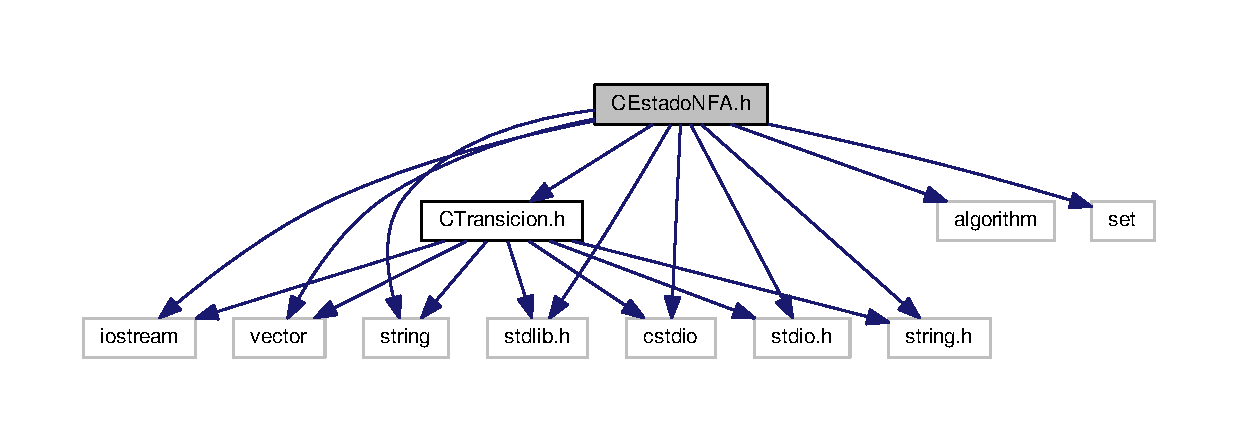
\includegraphics[width=350pt]{CEstadoNFA_8h__incl}
\end{center}
\end{figure}
This graph shows which files directly or indirectly include this file\+:
\nopagebreak
\begin{figure}[H]
\begin{center}
\leavevmode
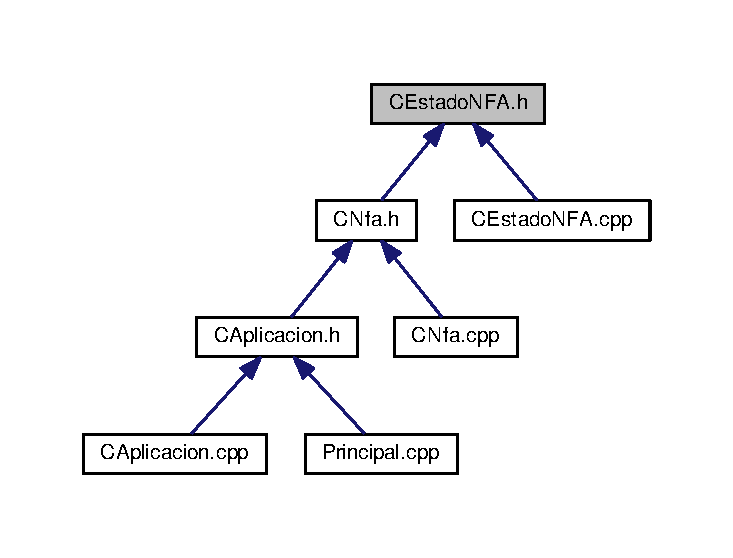
\includegraphics[width=350pt]{CEstadoNFA_8h__dep__incl}
\end{center}
\end{figure}
\subsection*{Classes}
\begin{DoxyCompactItemize}
\item 
class \hyperlink{classCEstado}{C\+Estado}
\end{DoxyCompactItemize}

\hypertarget{CFiltrosImagenes_8cpp}{}\section{C\+Filtros\+Imagenes.\+cpp File Reference}
\label{CFiltrosImagenes_8cpp}\index{C\+Filtros\+Imagenes.\+cpp@{C\+Filtros\+Imagenes.\+cpp}}
{\ttfamily \#include \char`\"{}C\+Filtros\+Imagenes.\+h\char`\"{}}\\*
Include dependency graph for C\+Filtros\+Imagenes.\+cpp\+:
\nopagebreak
\begin{figure}[H]
\begin{center}
\leavevmode
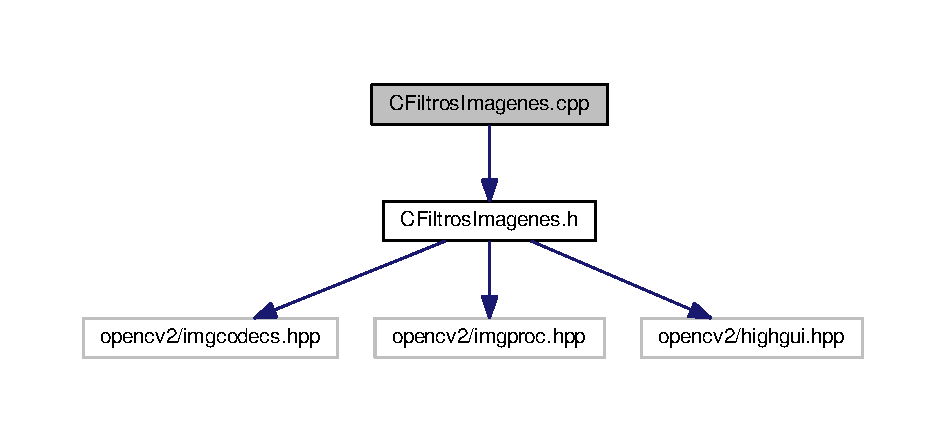
\includegraphics[width=350pt]{CFiltrosImagenes_8cpp__incl}
\end{center}
\end{figure}

\hypertarget{CFiltrosImagenes_8h}{}\section{C\+Filtros\+Imagenes.\+h File Reference}
\label{CFiltrosImagenes_8h}\index{C\+Filtros\+Imagenes.\+h@{C\+Filtros\+Imagenes.\+h}}
{\ttfamily \#include \char`\"{}opencv2/imgcodecs.\+hpp\char`\"{}}\\*
{\ttfamily \#include \char`\"{}opencv2/imgproc.\+hpp\char`\"{}}\\*
{\ttfamily \#include \char`\"{}opencv2/highgui.\+hpp\char`\"{}}\\*
Include dependency graph for C\+Filtros\+Imagenes.\+h\+:
\nopagebreak
\begin{figure}[H]
\begin{center}
\leavevmode
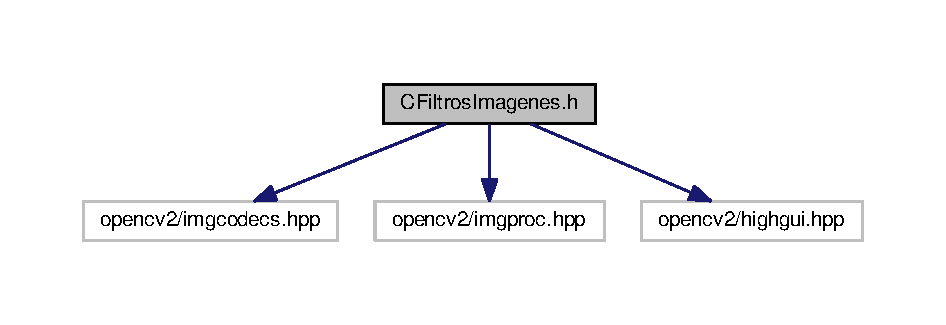
\includegraphics[width=350pt]{CFiltrosImagenes_8h__incl}
\end{center}
\end{figure}
This graph shows which files directly or indirectly include this file\+:
\nopagebreak
\begin{figure}[H]
\begin{center}
\leavevmode
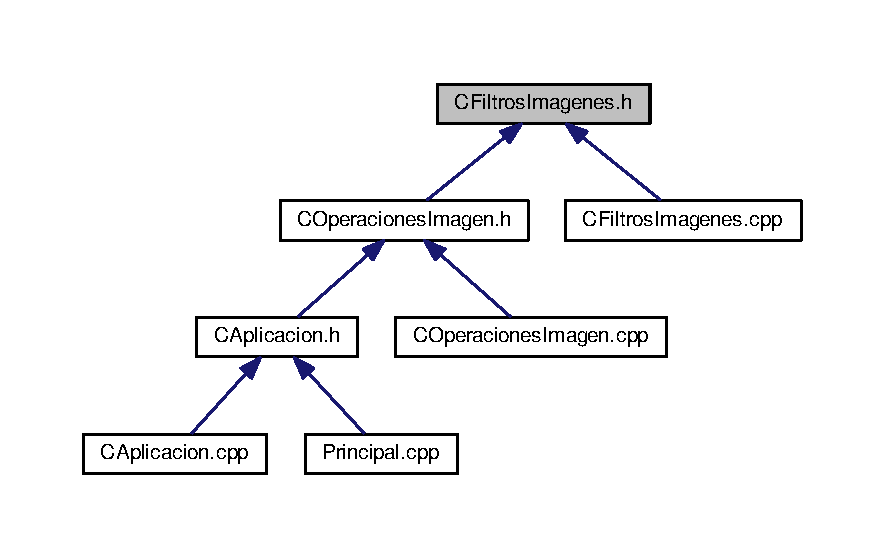
\includegraphics[width=350pt]{CFiltrosImagenes_8h__dep__incl}
\end{center}
\end{figure}
\subsection*{Classes}
\begin{DoxyCompactItemize}
\item 
class \hyperlink{classCFiltrosImagenes}{C\+Filtros\+Imagenes}
\begin{DoxyCompactList}\small\item\em Clase con diferentes filtros para aplicar sobre imagenes. \end{DoxyCompactList}\end{DoxyCompactItemize}

\hypertarget{CLabel_8cpp}{}\section{C\+Label.\+cpp File Reference}
\label{CLabel_8cpp}\index{C\+Label.\+cpp@{C\+Label.\+cpp}}
{\ttfamily \#include \char`\"{}C\+Label.\+h\char`\"{}}\\*
Include dependency graph for C\+Label.\+cpp\+:
\nopagebreak
\begin{figure}[H]
\begin{center}
\leavevmode
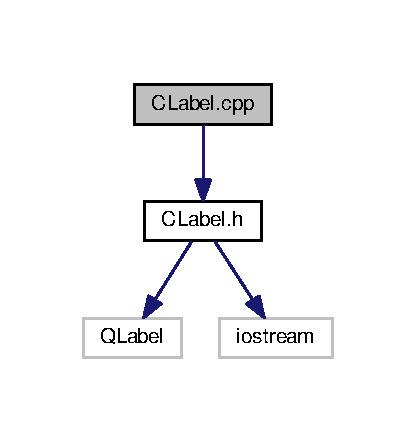
\includegraphics[width=320pt]{CLabel_8cpp__incl}
\end{center}
\end{figure}

\hypertarget{CLabel_8h}{}\section{C\+Label.\+h File Reference}
\label{CLabel_8h}\index{C\+Label.\+h@{C\+Label.\+h}}
{\ttfamily \#include $<$Q\+Label$>$}\\*
{\ttfamily \#include $<$iostream$>$}\\*
Include dependency graph for C\+Label.\+h\+:
\nopagebreak
\begin{figure}[H]
\begin{center}
\leavevmode
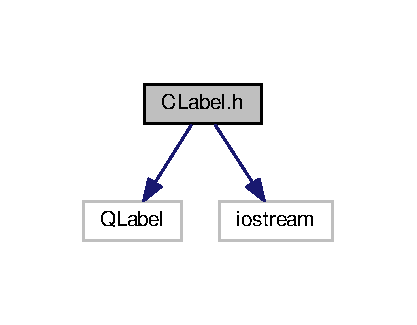
\includegraphics[width=200pt]{CLabel_8h__incl}
\end{center}
\end{figure}
This graph shows which files directly or indirectly include this file\+:
\nopagebreak
\begin{figure}[H]
\begin{center}
\leavevmode
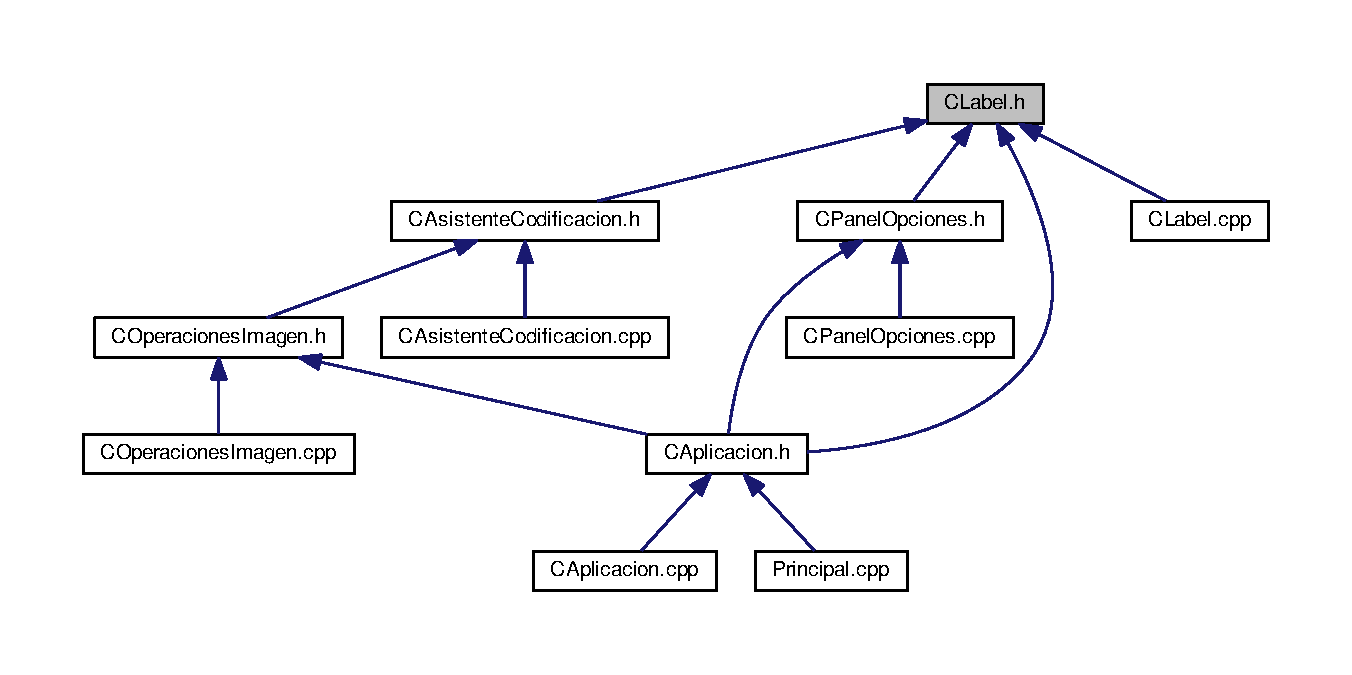
\includegraphics[width=350pt]{CLabel_8h__dep__incl}
\end{center}
\end{figure}
\subsection*{Classes}
\begin{DoxyCompactItemize}
\item 
class \hyperlink{classCLabel}{C\+Label}
\begin{DoxyCompactList}\small\item\em Clase heredada de \textquotesingle{}Q\+Label\textquotesingle{} que aplica un estilo determinado a este tipo de container. \end{DoxyCompactList}\end{DoxyCompactItemize}

\hypertarget{CLineEdit_8cpp}{}\section{C\+Line\+Edit.\+cpp File Reference}
\label{CLineEdit_8cpp}\index{C\+Line\+Edit.\+cpp@{C\+Line\+Edit.\+cpp}}
{\ttfamily \#include \char`\"{}C\+Line\+Edit.\+h\char`\"{}}\\*
Include dependency graph for C\+Line\+Edit.\+cpp\+:
\nopagebreak
\begin{figure}[H]
\begin{center}
\leavevmode
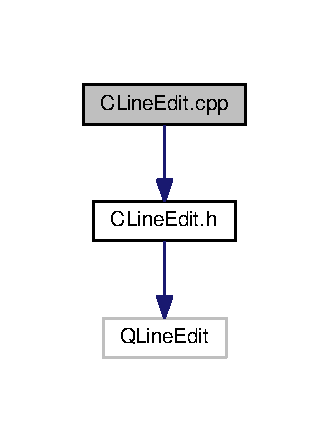
\includegraphics[width=158pt]{CLineEdit_8cpp__incl}
\end{center}
\end{figure}

\hypertarget{CLineEdit_8h}{}\section{C\+Line\+Edit.\+h File Reference}
\label{CLineEdit_8h}\index{C\+Line\+Edit.\+h@{C\+Line\+Edit.\+h}}
{\ttfamily \#include $<$Q\+Line\+Edit$>$}\\*
Include dependency graph for C\+Line\+Edit.\+h\+:
\nopagebreak
\begin{figure}[H]
\begin{center}
\leavevmode
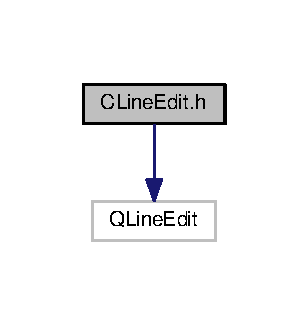
\includegraphics[width=148pt]{CLineEdit_8h__incl}
\end{center}
\end{figure}
This graph shows which files directly or indirectly include this file\+:
\nopagebreak
\begin{figure}[H]
\begin{center}
\leavevmode
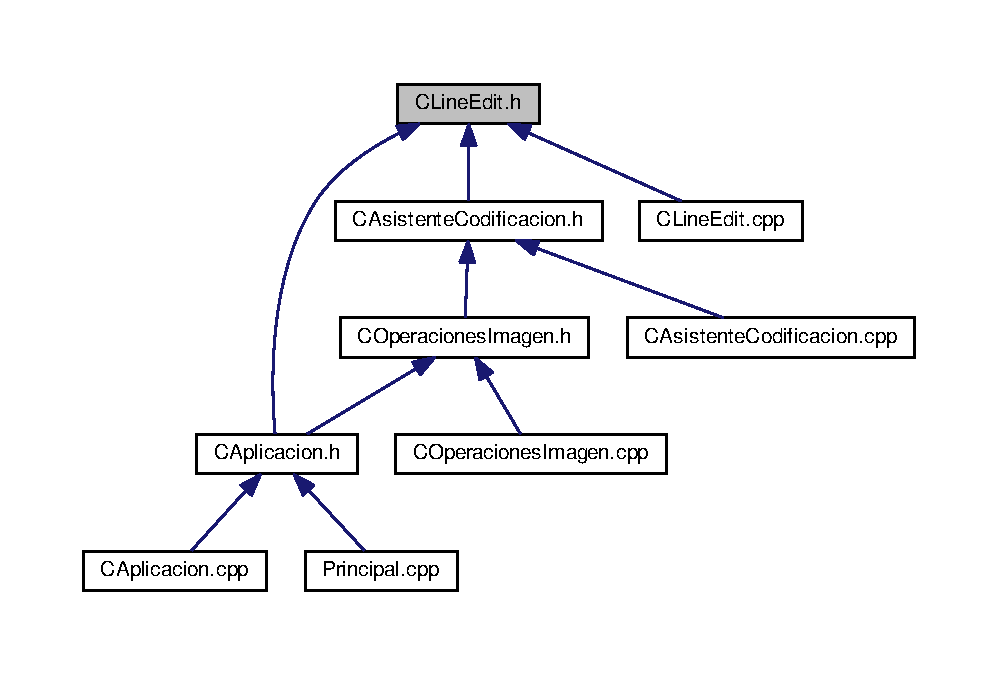
\includegraphics[width=350pt]{CLineEdit_8h__dep__incl}
\end{center}
\end{figure}
\subsection*{Classes}
\begin{DoxyCompactItemize}
\item 
class \hyperlink{classCLineEdit}{C\+Line\+Edit}
\begin{DoxyCompactList}\small\item\em Clase heredada de \textquotesingle{}Q\+Line\+Edit\textquotesingle{} que aplica un estilo determinado a este tipo de container. \end{DoxyCompactList}\end{DoxyCompactItemize}

\hypertarget{CNfa_8cpp}{}\section{C\+Nfa.\+cpp File Reference}
\label{CNfa_8cpp}\index{C\+Nfa.\+cpp@{C\+Nfa.\+cpp}}
{\ttfamily \#include $<$iostream$>$}\\*
{\ttfamily \#include $<$iterator$>$}\\*
{\ttfamily \#include $<$algorithm$>$}\\*
{\ttfamily \#include $<$set$>$}\\*
{\ttfamily \#include $<$vector$>$}\\*
{\ttfamily \#include $<$string$>$}\\*
{\ttfamily \#include $<$stdlib.\+h$>$}\\*
{\ttfamily \#include $<$cstdio$>$}\\*
{\ttfamily \#include $<$stdio.\+h$>$}\\*
{\ttfamily \#include $<$string.\+h$>$}\\*
{\ttfamily \#include \char`\"{}C\+Nfa.\+h\char`\"{}}\\*
{\ttfamily \#include $<$fstream$>$}\\*
{\ttfamily \#include $<$Q\+String$>$}\\*
{\ttfamily \#include $<$Q\+String\+List$>$}\\*
Include dependency graph for C\+Nfa.\+cpp\+:
\nopagebreak
\begin{figure}[H]
\begin{center}
\leavevmode
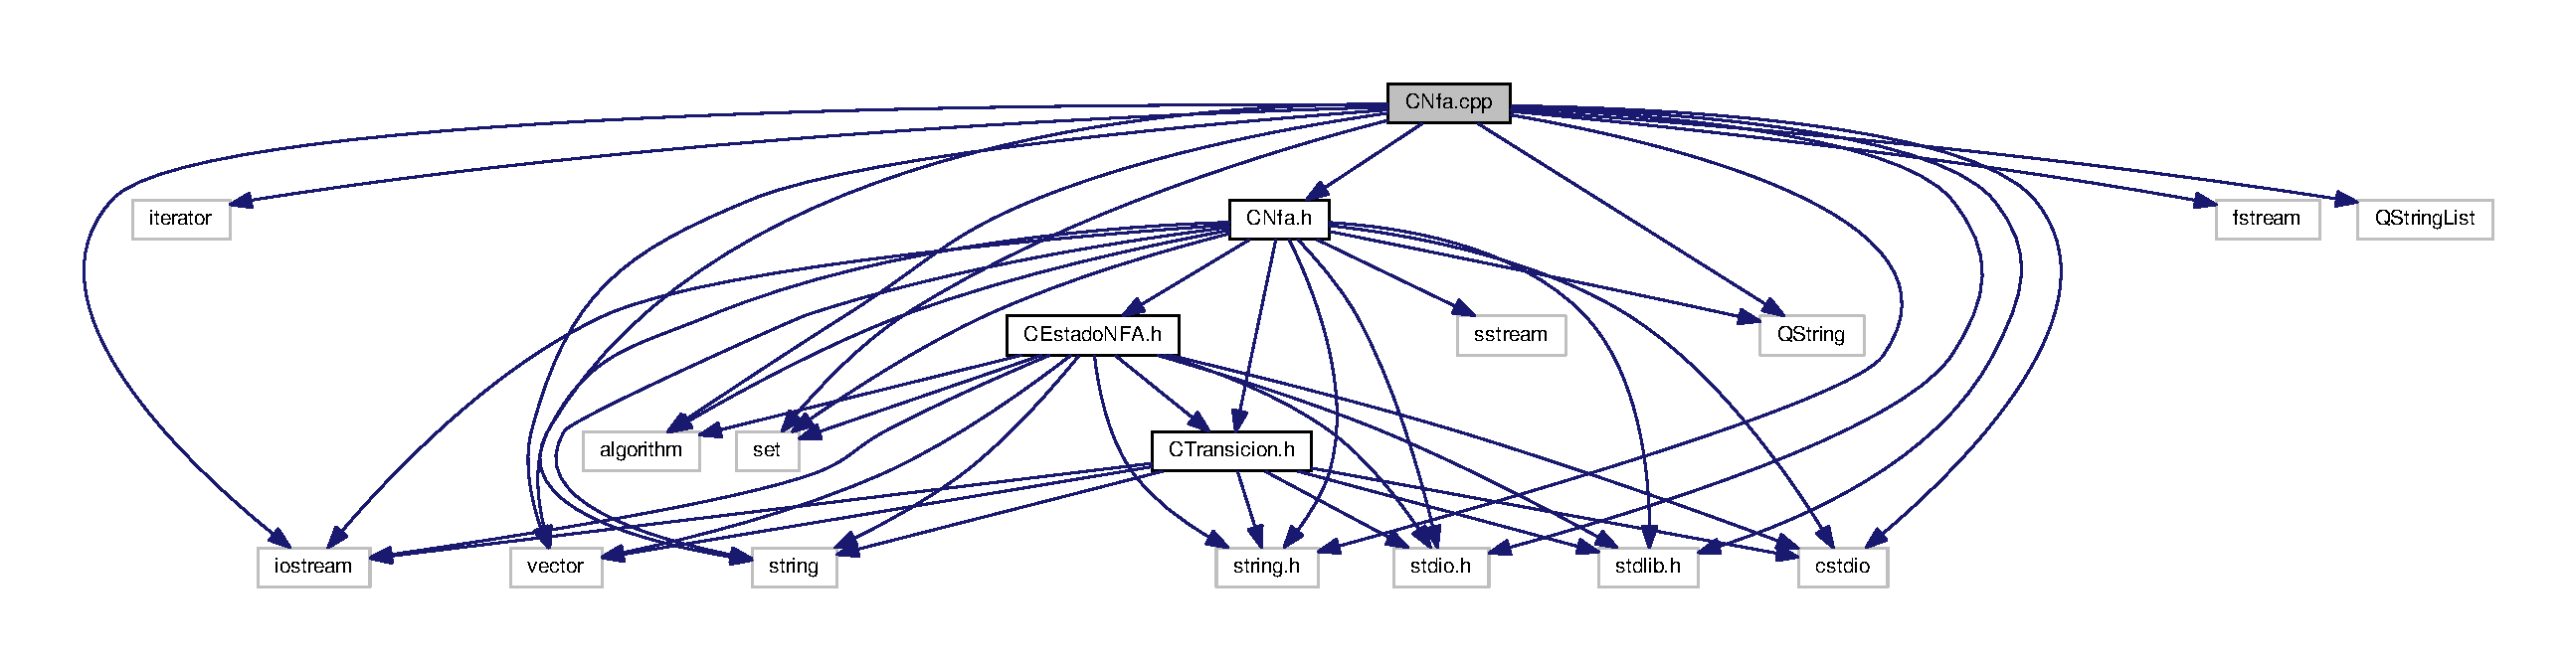
\includegraphics[width=350pt]{CNfa_8cpp__incl}
\end{center}
\end{figure}

\hypertarget{CNfa_8h}{}\section{C\+Nfa.\+h File Reference}
\label{CNfa_8h}\index{C\+Nfa.\+h@{C\+Nfa.\+h}}
{\ttfamily \#include $<$iostream$>$}\\*
{\ttfamily \#include $<$vector$>$}\\*
{\ttfamily \#include $<$set$>$}\\*
{\ttfamily \#include $<$string$>$}\\*
{\ttfamily \#include $<$stdlib.\+h$>$}\\*
{\ttfamily \#include $<$cstdio$>$}\\*
{\ttfamily \#include $<$stdio.\+h$>$}\\*
{\ttfamily \#include $<$string.\+h$>$}\\*
{\ttfamily \#include $<$algorithm$>$}\\*
{\ttfamily \#include $<$Q\+String$>$}\\*
{\ttfamily \#include \char`\"{}C\+Estado\+N\+F\+A.\+h\char`\"{}}\\*
{\ttfamily \#include \char`\"{}C\+Transicion.\+h\char`\"{}}\\*
{\ttfamily \#include $<$sstream$>$}\\*
Include dependency graph for C\+Nfa.\+h\+:
\nopagebreak
\begin{figure}[H]
\begin{center}
\leavevmode
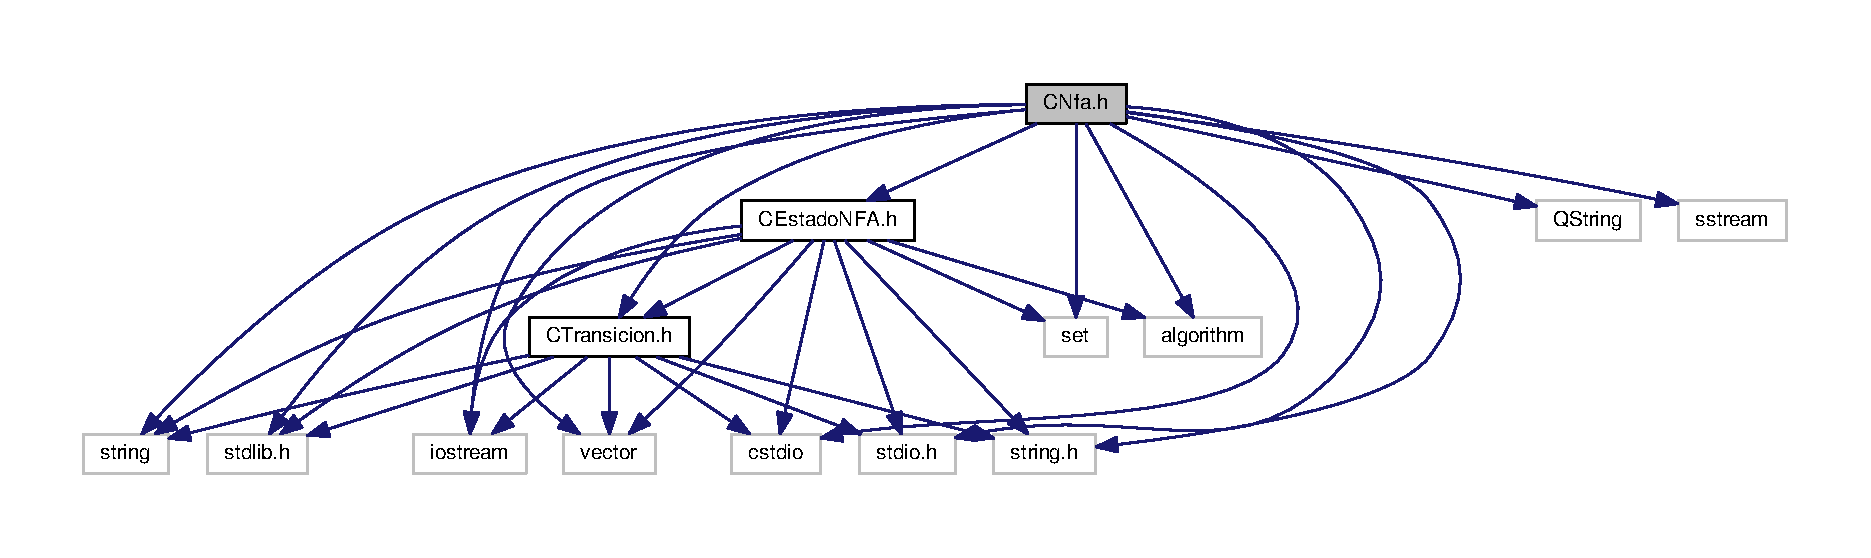
\includegraphics[width=350pt]{CNfa_8h__incl}
\end{center}
\end{figure}
This graph shows which files directly or indirectly include this file\+:
\nopagebreak
\begin{figure}[H]
\begin{center}
\leavevmode
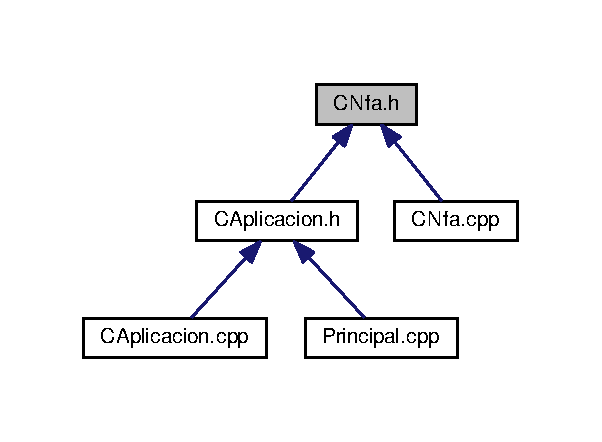
\includegraphics[width=289pt]{CNfa_8h__dep__incl}
\end{center}
\end{figure}
\subsection*{Classes}
\begin{DoxyCompactItemize}
\item 
class \hyperlink{classCNFA}{C\+N\+FA}
\end{DoxyCompactItemize}
\subsection*{Macros}
\begin{DoxyCompactItemize}
\item 
\#define \hyperlink{CNfa_8h_a5a090aad2cd0e647fe7995f80bcaedd5}{P\+A\+T\+H\+\_\+\+T\+E\+M\+P\+O\+R\+A\+L\+D\+FA}~\char`\"{}/home/ivan/Documentos/Codigo-\/T\+FG/codificaciones/temporal\+D\+F\+A.\+txt\char`\"{}
\end{DoxyCompactItemize}


\subsection{Macro Definition Documentation}
\index{C\+Nfa.\+h@{C\+Nfa.\+h}!P\+A\+T\+H\+\_\+\+T\+E\+M\+P\+O\+R\+A\+L\+D\+FA@{P\+A\+T\+H\+\_\+\+T\+E\+M\+P\+O\+R\+A\+L\+D\+FA}}
\index{P\+A\+T\+H\+\_\+\+T\+E\+M\+P\+O\+R\+A\+L\+D\+FA@{P\+A\+T\+H\+\_\+\+T\+E\+M\+P\+O\+R\+A\+L\+D\+FA}!C\+Nfa.\+h@{C\+Nfa.\+h}}
\subsubsection[{\texorpdfstring{P\+A\+T\+H\+\_\+\+T\+E\+M\+P\+O\+R\+A\+L\+D\+FA}{PATH_TEMPORALDFA}}]{\setlength{\rightskip}{0pt plus 5cm}\#define P\+A\+T\+H\+\_\+\+T\+E\+M\+P\+O\+R\+A\+L\+D\+FA~\char`\"{}/home/ivan/Documentos/Codigo-\/T\+FG/codificaciones/temporal\+D\+F\+A.\+txt\char`\"{}}\hypertarget{CNfa_8h_a5a090aad2cd0e647fe7995f80bcaedd5}{}\label{CNfa_8h_a5a090aad2cd0e647fe7995f80bcaedd5}

\hypertarget{COperacionesImagen_8cpp}{}\section{C\+Operaciones\+Imagen.\+cpp File Reference}
\label{COperacionesImagen_8cpp}\index{C\+Operaciones\+Imagen.\+cpp@{C\+Operaciones\+Imagen.\+cpp}}
{\ttfamily \#include \char`\"{}C\+Operaciones\+Imagen.\+h\char`\"{}}\\*
Include dependency graph for C\+Operaciones\+Imagen.\+cpp\+:
% FIG 0

\hypertarget{COperacionesImagen_8h}{}\section{C\+Operaciones\+Imagen.\+h File Reference}
\label{COperacionesImagen_8h}\index{C\+Operaciones\+Imagen.\+h@{C\+Operaciones\+Imagen.\+h}}
{\ttfamily \#include $<$iostream$>$}\\*
{\ttfamily \#include $<$fstream$>$}\\*
{\ttfamily \#include \char`\"{}opencv2/highgui.\+hpp\char`\"{}}\\*
{\ttfamily \#include \char`\"{}opencv2/imgcodecs.\+hpp\char`\"{}}\\*
{\ttfamily \#include \char`\"{}opencv2/imgproc.\+hpp\char`\"{}}\\*
{\ttfamily \#include \char`\"{}C\+Filtros\+Imagenes.\+h\char`\"{}}\\*
{\ttfamily \#include \char`\"{}C\+Detectar\+Circulos.\+h\char`\"{}}\\*
{\ttfamily \#include \char`\"{}C\+Detectar\+Lineas.\+h\char`\"{}}\\*
{\ttfamily \#include \char`\"{}C\+Detectar\+Transiciones.\+h\char`\"{}}\\*
{\ttfamily \#include \char`\"{}C\+Asistente\+Codificacion.\+h\char`\"{}}\\*
{\ttfamily \#include $<$Q\+Image$>$}\\*
Include dependency graph for C\+Operaciones\+Imagen.\+h\+:
% FIG 0
This graph shows which files directly or indirectly include this file\+:
% FIG 1
\subsection*{Classes}
\begin{DoxyCompactItemize}
\item 
class \hyperlink{classCOperacionesImagen}{C\+Operaciones\+Imagen}
\end{DoxyCompactItemize}
\subsection*{Macros}
\begin{DoxyCompactItemize}
\item 
\#define \hyperlink{COperacionesImagen_8h_a3f15382baa62393e05beea363392a85e}{D\+I\+S\+T\+A\+N\+C\+I\+A\+P\+I\+X\+E\+L\+S\+E\+C\+U\+N\+D\+A\+R\+IO}~100
\item 
\#define \hyperlink{COperacionesImagen_8h_a22ad15b01f07a0dc565e6931a4723c99}{C\+O\+N\+T\+O\+R\+N\+O\+M\+E\+D\+I\+O\+L\+E\+T\+RA}~30
\end{DoxyCompactItemize}


\subsection{Macro Definition Documentation}
\index{C\+Operaciones\+Imagen.\+h@{C\+Operaciones\+Imagen.\+h}!C\+O\+N\+T\+O\+R\+N\+O\+M\+E\+D\+I\+O\+L\+E\+T\+RA@{C\+O\+N\+T\+O\+R\+N\+O\+M\+E\+D\+I\+O\+L\+E\+T\+RA}}
\index{C\+O\+N\+T\+O\+R\+N\+O\+M\+E\+D\+I\+O\+L\+E\+T\+RA@{C\+O\+N\+T\+O\+R\+N\+O\+M\+E\+D\+I\+O\+L\+E\+T\+RA}!C\+Operaciones\+Imagen.\+h@{C\+Operaciones\+Imagen.\+h}}
\subsubsection[{\texorpdfstring{C\+O\+N\+T\+O\+R\+N\+O\+M\+E\+D\+I\+O\+L\+E\+T\+RA}{CONTORNOMEDIOLETRA}}]{\setlength{\rightskip}{0pt plus 5cm}\#define C\+O\+N\+T\+O\+R\+N\+O\+M\+E\+D\+I\+O\+L\+E\+T\+RA~30}\hypertarget{COperacionesImagen_8h_a22ad15b01f07a0dc565e6931a4723c99}{}\label{COperacionesImagen_8h_a22ad15b01f07a0dc565e6931a4723c99}
\index{C\+Operaciones\+Imagen.\+h@{C\+Operaciones\+Imagen.\+h}!D\+I\+S\+T\+A\+N\+C\+I\+A\+P\+I\+X\+E\+L\+S\+E\+C\+U\+N\+D\+A\+R\+IO@{D\+I\+S\+T\+A\+N\+C\+I\+A\+P\+I\+X\+E\+L\+S\+E\+C\+U\+N\+D\+A\+R\+IO}}
\index{D\+I\+S\+T\+A\+N\+C\+I\+A\+P\+I\+X\+E\+L\+S\+E\+C\+U\+N\+D\+A\+R\+IO@{D\+I\+S\+T\+A\+N\+C\+I\+A\+P\+I\+X\+E\+L\+S\+E\+C\+U\+N\+D\+A\+R\+IO}!C\+Operaciones\+Imagen.\+h@{C\+Operaciones\+Imagen.\+h}}
\subsubsection[{\texorpdfstring{D\+I\+S\+T\+A\+N\+C\+I\+A\+P\+I\+X\+E\+L\+S\+E\+C\+U\+N\+D\+A\+R\+IO}{DISTANCIAPIXELSECUNDARIO}}]{\setlength{\rightskip}{0pt plus 5cm}\#define D\+I\+S\+T\+A\+N\+C\+I\+A\+P\+I\+X\+E\+L\+S\+E\+C\+U\+N\+D\+A\+R\+IO~100}\hypertarget{COperacionesImagen_8h_a3f15382baa62393e05beea363392a85e}{}\label{COperacionesImagen_8h_a3f15382baa62393e05beea363392a85e}

\hypertarget{CPanelOpciones_8cpp}{}\section{C\+Panel\+Opciones.\+cpp File Reference}
\label{CPanelOpciones_8cpp}\index{C\+Panel\+Opciones.\+cpp@{C\+Panel\+Opciones.\+cpp}}
{\ttfamily \#include \char`\"{}C\+Panel\+Opciones.\+h\char`\"{}}\\*
Include dependency graph for C\+Panel\+Opciones.\+cpp\+:
\nopagebreak
\begin{figure}[H]
\begin{center}
\leavevmode
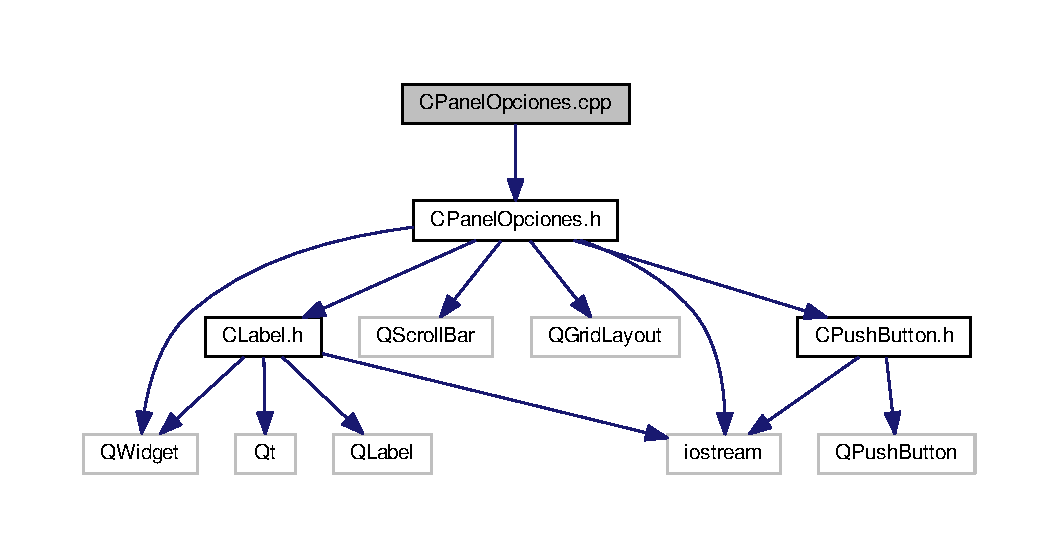
\includegraphics[width=350pt]{CPanelOpciones_8cpp__incl}
\end{center}
\end{figure}

\hypertarget{CPanelOpciones_8h}{}\section{C\+Panel\+Opciones.\+h File Reference}
\label{CPanelOpciones_8h}\index{C\+Panel\+Opciones.\+h@{C\+Panel\+Opciones.\+h}}
{\ttfamily \#include $<$Q\+Widget$>$}\\*
{\ttfamily \#include $<$Q\+Scroll\+Bar$>$}\\*
{\ttfamily \#include $<$Q\+Grid\+Layout$>$}\\*
{\ttfamily \#include \char`\"{}C\+Label.\+h\char`\"{}}\\*
Include dependency graph for C\+Panel\+Opciones.\+h\+:
% FIG 0
This graph shows which files directly or indirectly include this file\+:
% FIG 1
\subsection*{Classes}
\begin{DoxyCompactItemize}
\item 
class \hyperlink{classCPanelOpciones}{C\+Panel\+Opciones}
\end{DoxyCompactItemize}

\hypertarget{CPushButton_8cpp}{}\section{C\+Push\+Button.\+cpp File Reference}
\label{CPushButton_8cpp}\index{C\+Push\+Button.\+cpp@{C\+Push\+Button.\+cpp}}
{\ttfamily \#include \char`\"{}C\+Push\+Button.\+h\char`\"{}}\\*
Include dependency graph for C\+Push\+Button.\+cpp\+:
% FIG 0

\hypertarget{CPushButton_8h}{}\section{C\+Push\+Button.\+h File Reference}
\label{CPushButton_8h}\index{C\+Push\+Button.\+h@{C\+Push\+Button.\+h}}
{\ttfamily \#include $<$Q\+Push\+Button$>$}\\*
{\ttfamily \#include $<$iostream$>$}\\*
Include dependency graph for C\+Push\+Button.\+h\+:
\nopagebreak
\begin{figure}[H]
\begin{center}
\leavevmode
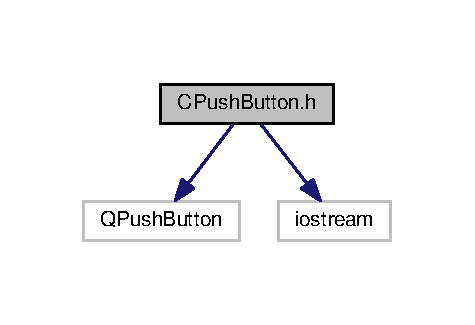
\includegraphics[width=228pt]{CPushButton_8h__incl}
\end{center}
\end{figure}
This graph shows which files directly or indirectly include this file\+:
\nopagebreak
\begin{figure}[H]
\begin{center}
\leavevmode
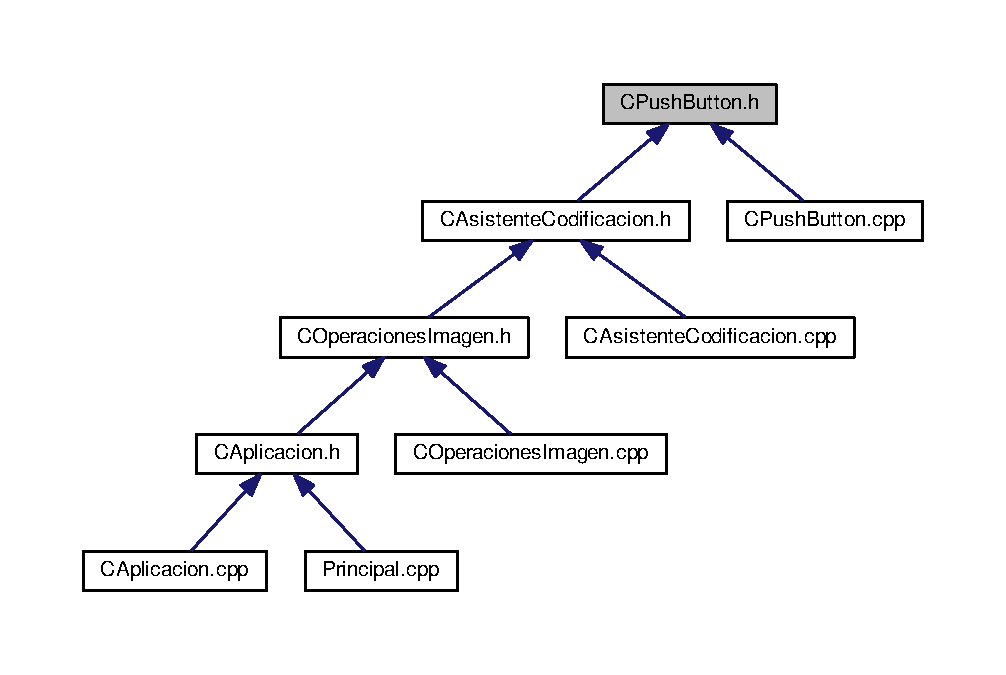
\includegraphics[width=350pt]{CPushButton_8h__dep__incl}
\end{center}
\end{figure}
\subsection*{Classes}
\begin{DoxyCompactItemize}
\item 
class \hyperlink{classCPushButton}{C\+Push\+Button}
\begin{DoxyCompactList}\small\item\em Clase heredada de \textquotesingle{}Q\+Push\+Button\textquotesingle{} que aplica un estilo determinado a este tipo de container. \end{DoxyCompactList}\end{DoxyCompactItemize}

\hypertarget{CTransicion_8cpp}{}\section{C\+Transicion.\+cpp File Reference}
\label{CTransicion_8cpp}\index{C\+Transicion.\+cpp@{C\+Transicion.\+cpp}}
{\ttfamily \#include \char`\"{}C\+Transicion.\+h\char`\"{}}\\*
{\ttfamily \#include $<$iostream$>$}\\*
{\ttfamily \#include $<$vector$>$}\\*
{\ttfamily \#include $<$string$>$}\\*
{\ttfamily \#include $<$stdlib.\+h$>$}\\*
{\ttfamily \#include $<$cstdio$>$}\\*
{\ttfamily \#include $<$stdio.\+h$>$}\\*
{\ttfamily \#include $<$string.\+h$>$}\\*
Include dependency graph for C\+Transicion.\+cpp\+:
\nopagebreak
\begin{figure}[H]
\begin{center}
\leavevmode
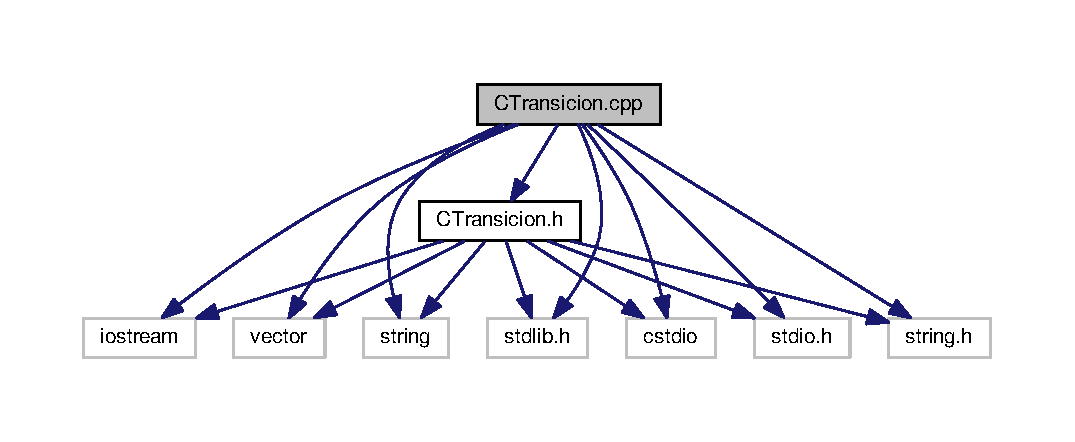
\includegraphics[width=350pt]{CTransicion_8cpp__incl}
\end{center}
\end{figure}

\hypertarget{CTransicion_8h}{}\section{C\+Transicion.\+h File Reference}
\label{CTransicion_8h}\index{C\+Transicion.\+h@{C\+Transicion.\+h}}
{\ttfamily \#include $<$iostream$>$}\\*
{\ttfamily \#include $<$vector$>$}\\*
{\ttfamily \#include $<$string$>$}\\*
{\ttfamily \#include $<$stdlib.\+h$>$}\\*
{\ttfamily \#include $<$cstdio$>$}\\*
{\ttfamily \#include $<$stdio.\+h$>$}\\*
{\ttfamily \#include $<$string.\+h$>$}\\*
Include dependency graph for C\+Transicion.\+h\+:
\nopagebreak
\begin{figure}[H]
\begin{center}
\leavevmode
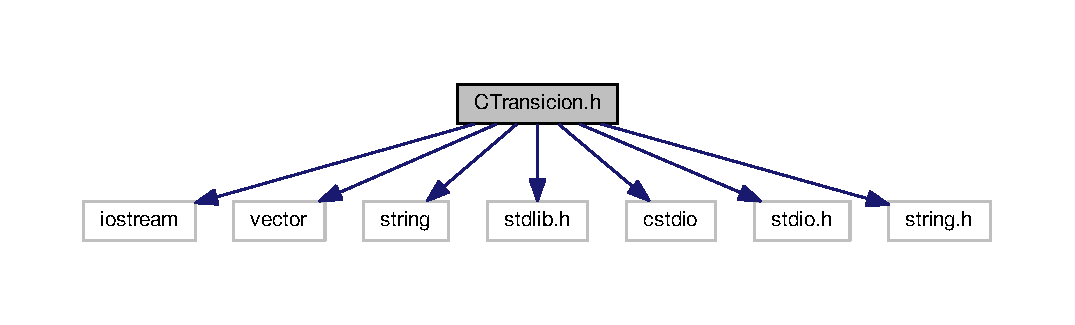
\includegraphics[width=350pt]{CTransicion_8h__incl}
\end{center}
\end{figure}
This graph shows which files directly or indirectly include this file\+:
\nopagebreak
\begin{figure}[H]
\begin{center}
\leavevmode
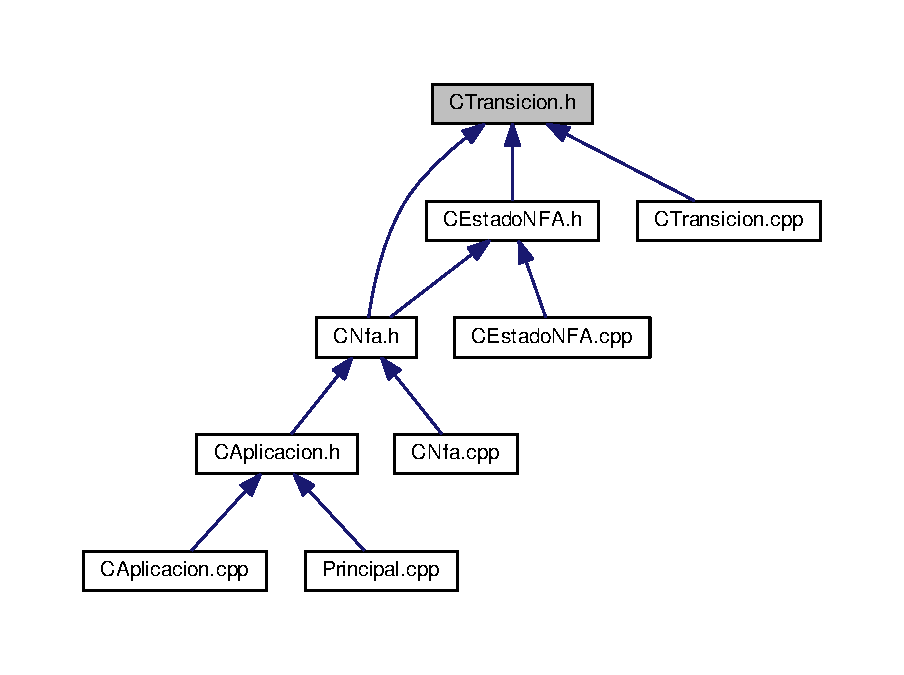
\includegraphics[width=350pt]{CTransicion_8h__dep__incl}
\end{center}
\end{figure}
\subsection*{Classes}
\begin{DoxyCompactItemize}
\item 
class \hyperlink{classCTransicion}{C\+Transicion}
\end{DoxyCompactItemize}

\hypertarget{DFA__min_8cpp}{}\section{D\+F\+A\+\_\+min.\+cpp File Reference}
\label{DFA__min_8cpp}\index{D\+F\+A\+\_\+min.\+cpp@{D\+F\+A\+\_\+min.\+cpp}}
{\ttfamily \#include \char`\"{}D\+F\+A\+\_\+min.\+h\char`\"{}}\\*
Include dependency graph for D\+F\+A\+\_\+min.\+cpp\+:
\nopagebreak
\begin{figure}[H]
\begin{center}
\leavevmode
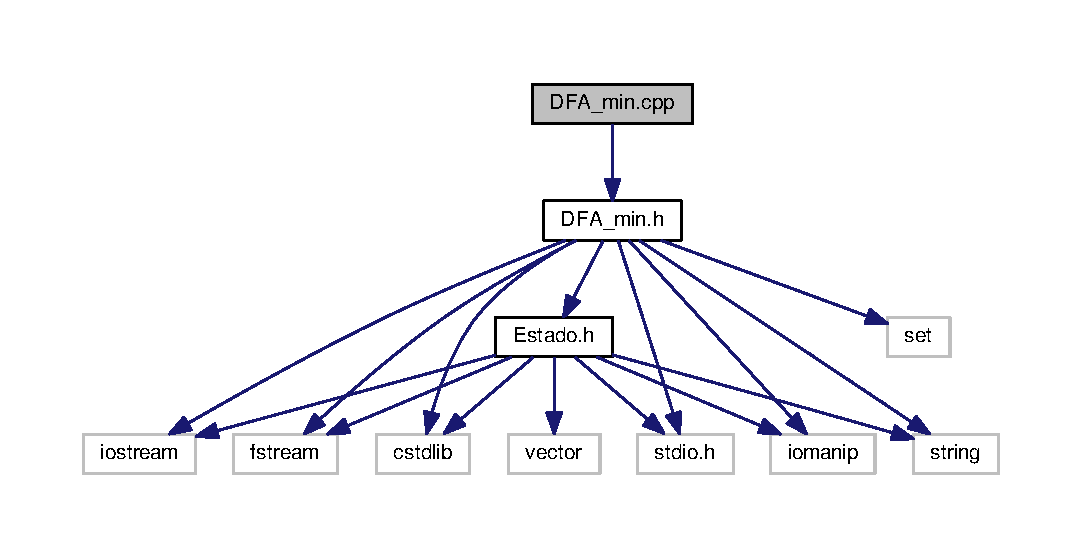
\includegraphics[width=350pt]{DFA__min_8cpp__incl}
\end{center}
\end{figure}
This graph shows which files directly or indirectly include this file\+:
\nopagebreak
\begin{figure}[H]
\begin{center}
\leavevmode
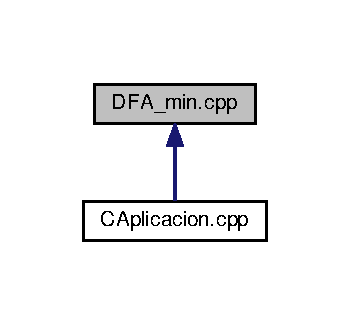
\includegraphics[width=168pt]{DFA__min_8cpp__dep__incl}
\end{center}
\end{figure}

\hypertarget{DFA__min_8h}{}\section{D\+F\+A\+\_\+min.\+h File Reference}
\label{DFA__min_8h}\index{D\+F\+A\+\_\+min.\+h@{D\+F\+A\+\_\+min.\+h}}
{\ttfamily \#include \char`\"{}Estado.\+h\char`\"{}}\\*
{\ttfamily \#include $<$iostream$>$}\\*
{\ttfamily \#include $<$fstream$>$}\\*
{\ttfamily \#include $<$cstdlib$>$}\\*
{\ttfamily \#include $<$stdio.\+h$>$}\\*
{\ttfamily \#include $<$iomanip$>$}\\*
{\ttfamily \#include $<$string$>$}\\*
{\ttfamily \#include $<$set$>$}\\*
Include dependency graph for D\+F\+A\+\_\+min.\+h\+:
\nopagebreak
\begin{figure}[H]
\begin{center}
\leavevmode
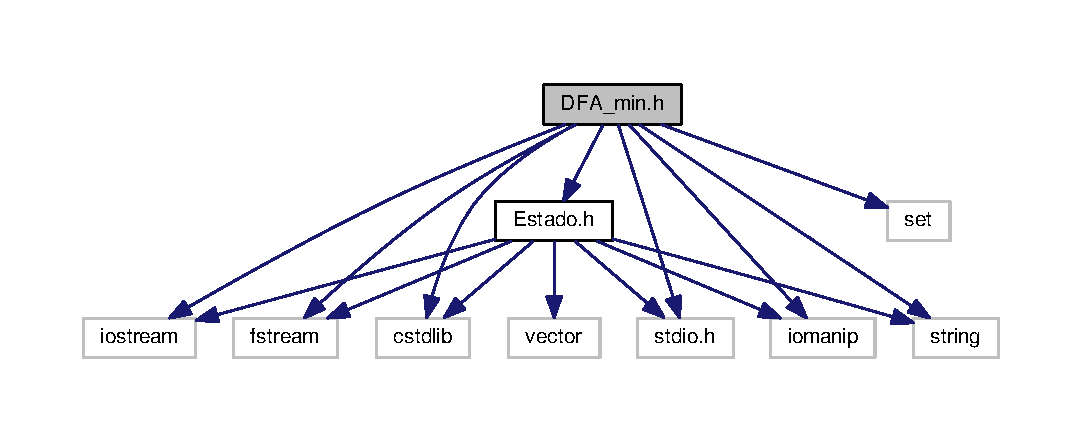
\includegraphics[width=350pt]{DFA__min_8h__incl}
\end{center}
\end{figure}
This graph shows which files directly or indirectly include this file\+:
\nopagebreak
\begin{figure}[H]
\begin{center}
\leavevmode
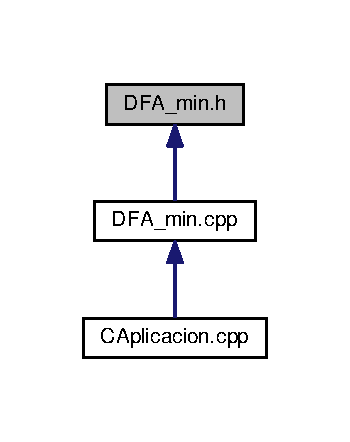
\includegraphics[width=168pt]{DFA__min_8h__dep__incl}
\end{center}
\end{figure}
\subsection*{Classes}
\begin{DoxyCompactItemize}
\item 
class \hyperlink{classDFA__MIN}{D\+F\+A\+\_\+\+M\+IN}
\end{DoxyCompactItemize}
\subsection*{Macros}
\begin{DoxyCompactItemize}
\item 
\#define \hyperlink{DFA__min_8h_a5a090aad2cd0e647fe7995f80bcaedd5}{P\+A\+T\+H\+\_\+\+T\+E\+M\+P\+O\+R\+A\+L\+D\+FA}~\char`\"{}/home/ivan/Documentos/Codigo-\/T\+FG/codificaciones/temporal\+D\+F\+A.\+txt\char`\"{}
\end{DoxyCompactItemize}


\subsection{Macro Definition Documentation}
\index{D\+F\+A\+\_\+min.\+h@{D\+F\+A\+\_\+min.\+h}!P\+A\+T\+H\+\_\+\+T\+E\+M\+P\+O\+R\+A\+L\+D\+FA@{P\+A\+T\+H\+\_\+\+T\+E\+M\+P\+O\+R\+A\+L\+D\+FA}}
\index{P\+A\+T\+H\+\_\+\+T\+E\+M\+P\+O\+R\+A\+L\+D\+FA@{P\+A\+T\+H\+\_\+\+T\+E\+M\+P\+O\+R\+A\+L\+D\+FA}!D\+F\+A\+\_\+min.\+h@{D\+F\+A\+\_\+min.\+h}}
\subsubsection[{\texorpdfstring{P\+A\+T\+H\+\_\+\+T\+E\+M\+P\+O\+R\+A\+L\+D\+FA}{PATH_TEMPORALDFA}}]{\setlength{\rightskip}{0pt plus 5cm}\#define P\+A\+T\+H\+\_\+\+T\+E\+M\+P\+O\+R\+A\+L\+D\+FA~\char`\"{}/home/ivan/Documentos/Codigo-\/T\+FG/codificaciones/temporal\+D\+F\+A.\+txt\char`\"{}}\hypertarget{DFA__min_8h_a5a090aad2cd0e647fe7995f80bcaedd5}{}\label{DFA__min_8h_a5a090aad2cd0e647fe7995f80bcaedd5}

\hypertarget{Estado_8cpp}{}\section{Estado.\+cpp File Reference}
\label{Estado_8cpp}\index{Estado.\+cpp@{Estado.\+cpp}}
{\ttfamily \#include \char`\"{}Estado.\+h\char`\"{}}\\*
Include dependency graph for Estado.\+cpp\+:
\nopagebreak
\begin{figure}[H]
\begin{center}
\leavevmode
\includegraphics[width=350pt]{Estado_8cpp__incl}
\end{center}
\end{figure}
This graph shows which files directly or indirectly include this file\+:
\nopagebreak
\begin{figure}[H]
\begin{center}
\leavevmode
\includegraphics[width=168pt]{Estado_8cpp__dep__incl}
\end{center}
\end{figure}

\hypertarget{Estado_8h}{}\section{Estado.\+h File Reference}
\label{Estado_8h}\index{Estado.\+h@{Estado.\+h}}
{\ttfamily \#include $<$iostream$>$}\\*
{\ttfamily \#include $<$fstream$>$}\\*
{\ttfamily \#include $<$cstdlib$>$}\\*
{\ttfamily \#include $<$stdio.\+h$>$}\\*
{\ttfamily \#include $<$iomanip$>$}\\*
{\ttfamily \#include $<$vector$>$}\\*
{\ttfamily \#include $<$string$>$}\\*
Include dependency graph for Estado.\+h\+:
\nopagebreak
\begin{figure}[H]
\begin{center}
\leavevmode
\includegraphics[width=350pt]{Estado_8h__incl}
\end{center}
\end{figure}
This graph shows which files directly or indirectly include this file\+:
\nopagebreak
\begin{figure}[H]
\begin{center}
\leavevmode
\includegraphics[width=242pt]{Estado_8h__dep__incl}
\end{center}
\end{figure}
\subsection*{Classes}
\begin{DoxyCompactItemize}
\item 
class \hyperlink{classEstado}{Estado}
\end{DoxyCompactItemize}

\hypertarget{GenerarClasificador_8cpp}{}\section{Generar\+Clasificador.\+cpp File Reference}
\label{GenerarClasificador_8cpp}\index{Generar\+Clasificador.\+cpp@{Generar\+Clasificador.\+cpp}}

\hypertarget{Principal_8cpp}{}\section{Principal.\+cpp File Reference}
\label{Principal_8cpp}\index{Principal.\+cpp@{Principal.\+cpp}}
{\ttfamily \#include \char`\"{}C\+Aplicacion.\+h\char`\"{}}\\*
Include dependency graph for Principal.\+cpp\+:
\nopagebreak
\begin{figure}[H]
\begin{center}
\leavevmode
\includegraphics[width=350pt]{Principal_8cpp__incl}
\end{center}
\end{figure}
\subsection*{Functions}
\begin{DoxyCompactItemize}
\item 
int \hyperlink{Principal_8cpp_a0ddf1224851353fc92bfbff6f499fa97}{main} (int argc, char $\ast$argv\mbox{[}$\,$\mbox{]})
\end{DoxyCompactItemize}


\subsection{Function Documentation}
\index{Principal.\+cpp@{Principal.\+cpp}!main@{main}}
\index{main@{main}!Principal.\+cpp@{Principal.\+cpp}}
\subsubsection[{\texorpdfstring{main(int argc, char $\ast$argv[])}{main(int argc, char *argv[])}}]{\setlength{\rightskip}{0pt plus 5cm}int main (
\begin{DoxyParamCaption}
\item[{int}]{argc, }
\item[{char $\ast$}]{argv\mbox{[}$\,$\mbox{]}}
\end{DoxyParamCaption}
)}\hypertarget{Principal_8cpp_a0ddf1224851353fc92bfbff6f499fa97}{}\label{Principal_8cpp_a0ddf1224851353fc92bfbff6f499fa97}

\hypertarget{prueba_8cpp}{}\section{prueba.\+cpp File Reference}
\label{prueba_8cpp}\index{prueba.\+cpp@{prueba.\+cpp}}

\hypertarget{prueba_8txt_8txt}{}\section{prueba.\+txt.\+txt File Reference}
\label{prueba_8txt_8txt}\index{prueba.\+txt.\+txt@{prueba.\+txt.\+txt}}

\hypertarget{pruebablobs_8cpp}{}\section{pruebablobs.\+cpp File Reference}
\label{pruebablobs_8cpp}\index{pruebablobs.\+cpp@{pruebablobs.\+cpp}}

\hypertarget{pruebalineas_8cpp}{}\section{pruebalineas.\+cpp File Reference}
\label{pruebalineas_8cpp}\index{pruebalineas.\+cpp@{pruebalineas.\+cpp}}

\hypertarget{pruebanumeros_8cpp}{}\section{pruebanumeros.\+cpp File Reference}
\label{pruebanumeros_8cpp}\index{pruebanumeros.\+cpp@{pruebanumeros.\+cpp}}

\hypertarget{README_8md}{}\section{R\+E\+A\+D\+M\+E.\+md File Reference}
\label{README_8md}\index{R\+E\+A\+D\+M\+E.\+md@{R\+E\+A\+D\+M\+E.\+md}}

\hypertarget{uiprueba_8cpp}{}\section{uiprueba.\+cpp File Reference}
\label{uiprueba_8cpp}\index{uiprueba.\+cpp@{uiprueba.\+cpp}}

%--- End generated contents ---

% Index
\backmatter
\newpage
\phantomsection
\clearemptydoublepage
\addcontentsline{toc}{chapter}{Index}
\printindex

\end{document}
